\documentclass[12pt,letterpaper]{article}
% Draft 2, 2026-11-16. Original draft: wdj and C. Melles, 2023-03-26.
% Draft 1 (2026-11-15): corrections from a computational referee check.
% Draft 2 (2026-11-16): revision to the authors' style guide. See revision-log.tex.
\usepackage[T1]{fontenc}
\IfFileExists{newtxmath.sty}{\usepackage{newtxtext,newtxmath}}{\usepackage{mathptmx}}
\usepackage[letterpaper,margin=1in]{geometry}
\usepackage{amsmath,amssymb,amsthm}
\usepackage{float}
\usepackage{graphicx}
\usepackage{url}
\usepackage{fancyvrb}
\usepackage{makeidx}
\usepackage{cprotect}
\usepackage{microtype}
\usepackage[hidelinks]{hyperref}
\def\UrlBreaks{\do\/\do\_\do\.\do\-}

\newtheorem{theorem}{Theorem}[section]
\newtheorem{corollary}[theorem]{Corollary}
\newtheorem{conjecture}[theorem]{Conjecture}
\newtheorem{lemma}[theorem]{Lemma}
\newtheorem{proposition}[theorem]{Proposition}
\theoremstyle{definition}
\newtheorem{definition}[theorem]{Definition}
\newtheorem{example}[theorem]{Example}
\newtheorem{remark}[theorem]{Remark}
\newtheorem{revremark}{Remark}
\renewcommand{\therevremark}{2026.\arabic{revremark}}

\DeclareMathOperator{\Aut}{Aut}
\DeclareMathOperator{\genus}{genus}
\DeclareMathOperator{\Jac}{Jac}

\def\ppp{{\mathbb{P}}}
\def\hhh{{\mathbb{H}}}
\def\aaa{{\mathbb{A}}}
\def\fff{{\mathbb{F}}}
\def\qqq{\mathbb{Q}}
\def\rrr{\mathbb{R}}
\def\ccc{\mathbb{C}}
\def\zzz{\mathbb{Z}}
\def\nnn{\mathbb{N}}

\makeindex

\begin{document}


\title{Harmonic quotient morphisms of regular graphs: examples\thanks{The
original draft of this paper is an unpublished manuscript by the authors,
dated March 26, 2023. Draft~1 (November 15, 2026) corrected errors found by
a computational referee check. Draft~2 (November 16, 2026) revises the paper
to the authors' style guide. The repository
\url{https://github.com/wdjoyner/alg-graph-thry}, folder
{\tt harmonic-quotient}, contains all drafts, a revision log and the
verification scripts.}}
\author{David Joyner\\ {\small\tt wdjoyner@gmail.com} \and Caroline Melles}
\date{Original draft: March 26, 2023. Corrected draft: November 16, 2026 (Draft 2).}
\maketitle

\begin{abstract}
We give many examples of harmonic morphisms $\phi:\Gamma_2\to\Gamma_1$ in the sense
of Baker and Norine, where $\Gamma_2$ is a connected $k$-regular graph
($k=3,4,5$) with at most $12$ vertices. For each graph we record standard
invariants and the number of harmonic morphisms to several small graphs. We
emphasize harmonic quotient morphisms $\Gamma_2\to\Gamma_2/G$, where $G$ is a
subgroup of $\Aut(\Gamma_2)$. For most graphs we list all such quotients and
tabulate one example of each kind. All counts are the results of exhaustive
computer searches. This corrected draft fixes errors found by an independent
recomputation of every table, count and invariant.
\end{abstract}

\vskip .2in

\tableofcontents

\section{Introduction}
\label{sec:introduction}

This section states the problem, explains why it is of interest, and
summarizes what the paper contains.

A harmonic morphism of graphs is the graph-theoretic analogue of a
holomorphic map between Riemann surfaces \cite{Ur00,BN09}. A rich source of
such maps is the quotient of a graph by a group of its automorphisms. If
$G\subseteq\Aut(\Gamma_2)$, the quotient map $\pi:\Gamma_2\to\Gamma_2/G$ sends
each vertex to its orbit. This map is sometimes harmonic and sometimes not.
When it is harmonic, the target $\Gamma_2/G$ inherits some of the structure
of $\Gamma_2$. For example, the critical group of $\Gamma_2/G$ is then a
quotient of the critical group of $\Gamma_2$ (Lemma~\ref{lemma:jacobian}).

This paper is a catalogue of examples. All graphs are simple and connected.
We take $\Gamma_2$ to be a $k$-regular graph with a ``small'' number of
vertices. The cubic graphs with $6$, $8$, $10$ and $12$ vertices are treated
in Section~\ref{sec:cubic-examples}. Selected quartic graphs with $5$ to $12$
vertices are treated in Section~\ref{sec:quartic-examples}. Selected quintic
graphs with $6$, $8$ and $10$ vertices are treated in
Section~\ref{sec:quintic-examples}. For each graph we record its
characteristic polynomial, diameter, girth, circumference, automorphism
group order and critical group order. We also count the non-trivial
harmonic morphisms to several small graphs, such as $P_3$, $P_4$, $St_4$,
$C_3$, $C_4$ and $K_4$. For most graphs we then list all harmonic quotient
morphisms and tabulate one representative of each kind.

The examples were collected with one question in mind.

\vskip .1in
\noindent
{\bf Question}: Which regular graphs $\Gamma_2$ have no (or very few)
harmonic quotients other than $P_2$?
\vskip .1in

For example, look at $K_5$ and {\tt d5reg10a} below.
Section~\ref{sec:summary} collects what the examples say about this question.

\paragraph{Status of the results.}
Apart from the elementary lemmas in Section~\ref{sec:background}, every
statement about a specific graph in this paper is a computational result.
These results come from exhaustive and exact computer searches. They are
not proved by hand. The original computations used the Sage functions in
the file \path{alg-graph-thry2.sage} of the repository
\url{https://github.com/wdjoyner/alg-graph-thry} (commit {\tt 538896d}).
For this draft every table, count and graph invariant was recomputed by
independent programs that do not use those functions. They are in the
folder \path{harmonic-quotient/verification} of the same repository (commit
{\tt 295fd16}). They use NetworkX, GAP \cite{GAP} and nauty \cite{MP14}.
Section~\ref{sec:computations} describes both computations.

\paragraph{What is new in the 2026 revision.}
The original draft of March 26, 2023 is kept in the repository. The 2026
revision corrects errors and adds material. Three kinds of statement are
new. First, the counts of distinct morphisms in the quotient lists (for
example in Examples~\ref{example:d3reg10n} and~\ref{example:d4reg12a}).
Second, the quotients for $G=\Aut(\Gamma_2)$, which the original search
omitted (Remark~\ref{rem:full-group}). Third, Sections~\ref{sec:introduction}
to~\ref{sec:notation}, \ref{sec:summary} and~\ref{sec:glossary}. The revision
log in the repository lists every individual change.

\section{Literature review}
\label{sec:literature}

This section summarizes the work that this paper builds on and says how
the examples fit in. Work that appeared before the original draft (March
26, 2023) is reviewed first. Later work follows.

\subsection{Work before 2023}

Urakawa \cite{Ur00} introduced harmonic morphisms between simple graphs as
maps that pull back harmonic functions to harmonic functions. He showed that
such a map sends adjacent vertices to adjacent or equal vertices and is
horizontally conformal. His motivation was the stochastic picture: a
harmonic morphism sends random walks to random walks up to a time change.

Baker and Norine \cite{BN09} extended the definition to multigraphs and
developed it as a discrete analogue of holomorphic maps. They defined the
degree and the horizontal and vertical multiplicities, proved a
Riemann--Hurwitz formula, and showed that a non-constant harmonic morphism
induces a surjection of Jacobians. Their definitions are the ones used here.
Hyperelliptic graphs, studied in \cite{BN09}, are graphs of genus at least
$2$ with an involution whose quotient morphism is harmonic with a tree as
target. Several examples below are of this kind.

Corry \cite{Co11} defined harmonic group actions on graphs. These are group
actions whose quotient morphism is harmonic. He proved that the largest such
group acting on a graph of genus $g\geq 2$ has order between $4(g-1)$ and
$6(g-1)$, and that both bounds are attained infinitely often. He then
classified harmonic branched $G$-covers of a fixed base graph \cite{Co12} and
described the graphs and groups that attain the upper bound \cite{Co15}. The
present paper studies the same quotient morphisms from the opposite end. It
fixes a small regular graph and lists every subgroup of its automorphism
group whose quotient morphism is harmonic. Corry's quotient graph keeps one
edge for each orbit of edges. Our quotient graph is simple (see
Section~\ref{sec:quotients}), so the two notions of harmonic quotient need
not agree.

Several of the graphs below are circulant. Mednykh and Mednykh
\cite{MM19} gave explicit formulas for the number of spanning trees of
circulant graphs, and these numbers are the critical group orders recorded
below. Bussemaker and Cvetkovi\'c \cite{BC76} showed that there are exactly
$13$ connected cubic integral graphs. Some of them appear here. The authors'
book \cite{JM17} contains background on graphs, Laplacians and critical
groups. Their manuscript \cite{MJ22} develops harmonic morphisms in detail.

\subsection{Work since 2023}

Meyer and Zakharov \cite{MZ23} defined the Jacobian of a graph of groups.
For a group acting on a graph they defined pushforward and pullback maps
between the Jacobian of the graph and that of the quotient graph of groups.
Vetluzhskikh and Zakharov \cite{VZ24} studied the kernel of the
pushforward map on critical groups for harmonic covers with abelian Galois
group. They computed its order with Zaslavsky's bias matroid. These papers
explain, in the abelian case, how much of the critical group of $\Gamma_2$
survives in a harmonic quotient. The divisibility test of
Lemma~\ref{lemma:jacobian} is the crudest form of this information.

Archer and Melles \cite{AM25} showed that arithmetical structures can be
pulled back along harmonic morphisms, and proved a Riemann--Hurwitz formula
for arithmetical structures. Melles and Joyner \cite{MJ26} give a book-length
treatment of harmonic morphisms, with an emphasis on computation.

\section{Background}
\label{sec:background}

This section collects the definitions and facts that the examples rely on.
It fixes conventions for graphs, defines harmonic morphisms and harmonic
quotients, proves three elementary lemmas that are used repeatedly, and
describes how the data were computed.

\subsection{Graph-theoretic conventions}
\label{sec:conventions}


We will always assume we have fixed an indexing of the vertices $V$ and
edges $E$ of a graph $\Gamma = (V,E)$.
Typically, the vertices are represented as $V = \{0, 1, \dots , n - 1\}$
and the edges are represented by pairs $(u, v)$, where $u < v$
are the vertices in $V$ incident to that edge.
In this situation we say $\Gamma$ is in {\it standard form}.
\index{standard form}

Recall a graph $\Gamma=(V,E)$ with automorphism group $G$ is
called {\it vertex transitive} if $G$ acts transitively on $V$.
It is called {\it edge transitive} if $G$ acts transitively on $E$.
We distinguish between (unoriented) edges and arcs, which are
oriented with a head and a tail. A graph is {\it arc transitive},
or {\it symmetric}, if $G$ acts transitively on the set of arcs
of $\Gamma$.
\index{vertex transitive graph}
\index{edge transitive graph}
\index{arc transitive graph}
Recall a
graph is called {\it Hamiltonian} if there is a simple closed path
containing each vertex of the graph.
\index{Hamiltonian graph}

A {\it circulant graph} with parameters $(n,L)$ is a
graph $\Gamma=(V,E)$ in standard form\footnote{We identify the
vertices $V=\{0,1,\dots,n-1\}$ with the cyclic group
$\zzz/n\zzz$ and $L\subset V$.} with the property
that each vertex $i$ is adjacent to
the vertices $i+j$ and $i-j$ for each $j \in L$.
\index{circulant graph}

Generally, the barbell graph $\mathrm{Barbell}(n_1, n_2)$
is a graph with $2n_1 + n_2$ vertices ($n_1>2$, $n_2\geq 0$),
that consists of a path graph $P_{n_2+2}$ connecting two complete graphs
$K_{n_1}$.
\index{barbell graph}



\subsection{Harmonic morphisms}
\label{sec:harmonic-morphisms}

This subsection gives the definition of a harmonic morphism used throughout,
together with the quantities recorded in every table.

The definition is designed so that harmonic functions pull back to harmonic
functions, as for holomorphic maps of Riemann surfaces \cite{Ur00}. Baker and
Norine \cite[\S2.1]{BN09} reformulated it as a local counting condition,
which is what we use. Since all our graphs are simple, a morphism is
determined by its map on vertices.

\begin{definition}
\label{def:harmonic}
Let $\Gamma_2=(V_2,E_2)$ and $\Gamma_1=(V_1,E_1)$ be simple graphs. A map
$\phi:V_2\to V_1$ is a {\it morphism} if for every edge $uv\in E_2$ either
$\phi(u)=\phi(v)$ or $\phi(u)\phi(v)\in E_1$. In the first case the edge $uv$
is {\it vertical}, and in the second case it is {\it horizontal}. For
$x\in V_2$ and a neighbor $w$ of $\phi(x)$ in $\Gamma_1$, let $m_\phi(x,w)$ be
the number of neighbors $y$ of $x$ with $\phi(y)=w$. The morphism is
{\it harmonic} if, for each $x\in V_2$, the number $m_\phi(x,w)$ does not
depend on $w$. This common value is the {\it horizontal multiplicity}
$m_\phi(x)$. The {\it vertical multiplicity} $\nu_\phi(x)$ is the number of
neighbors $y$ of $x$ with $\phi(y)=\phi(x)$.
\end{definition}
\index{harmonic morphism}
\index{horizontal multiplicity}
\index{vertical multiplicity}

We list a harmonic morphism as the sequence
$(\phi(0),\phi(1),\dots,\phi(n-1))$, sometimes called its {\it CL format}.
Each table in this paper lists $x$, $\phi(x)$, $m_\phi(x)$ and $\nu_\phi(x)$
for every vertex $x$ of $\Gamma_2$.

For a harmonic morphism $\phi$ and an edge $e'$ of $\Gamma_1$, the number of
edges of $\Gamma_2$ mapped onto $e'$ does not depend on $e'$
\cite[Lemma~2.4]{BN09}. This number is the {\it degree} $\deg(\phi)$. For any
vertex $v$ of $\Gamma_1$ it equals
\[
\deg(\phi)=\sum_{x\in\phi^{-1}(v)} m_\phi(x).
\]
A non-constant harmonic morphism to a connected graph is surjective
\cite[Lemma~2.7]{BN09}. In this paper a {\it non-trivial} harmonic
morphism is a non-constant one. Counts of non-trivial harmonic morphisms
count vertex maps, so two morphisms that differ by an automorphism of
$\Gamma_1$ are counted separately.

The {\it genus} of a connected graph $\Gamma=(V,E)$ is
$\genus(\Gamma)=|E|-|V|+1$. The Riemann--Hurwitz formula
\cite[Theorem~2.14]{BN09} relates the genera of the two graphs:
\[
2\genus(\Gamma_2)-2=\deg(\phi)\,\bigl(2\genus(\Gamma_1)-2\bigr)
+\sum_{x\in V_2}\bigl(2(m_\phi(x)-1)+\nu_\phi(x)\bigr).
\]
Every table in this paper satisfies this formula. When
$\genus(\Gamma_1)\neq 1$ it determines $\deg(\phi)$ from the other entries.
(Theorem and lemma numbers for \cite{BN09} refer to arXiv:0707.1309v2.)

\begin{example}
\label{example:rh-star}
Let $\Gamma_2=K_{3,3}$ with parts $\{0,2,4\}$ and $\{1,3,5\}$. Map $0,2,4$ to
the center of the star $St_4$ and map $1,3,5$ bijectively to its three
leaves. Each vertex $0,2,4$ has one neighbor over each leaf, so
$m_\phi=1$ there. Each vertex $1,3,5$ has three neighbors over the center,
so $m_\phi=3$ there. There are no vertical edges. The degree is $3$. The
Riemann--Hurwitz formula reads $2\cdot 4-2=3\cdot(-2)+3\cdot 0+3\cdot 4$.
\end{example}

The following terms describe the shape of a harmonic morphism. We use them
as in the original draft.

\begin{definition}
\label{def:covers}
A harmonic morphism $\phi$ is a {\it homomorphism} if it has no vertical
edges, that is $\nu_\phi\equiv 0$. It is a {\it cover} if $m_\phi\equiv 1$
and $\nu_\phi\equiv 0$, and a {\it quasicover} if $m_\phi\equiv 1$. It is an
{\it $m$-multicover} if $m_\phi\equiv m$ and $\nu_\phi\equiv 0$, and a
{\it quasi-$m$-multicover} if $m_\phi\equiv m$.
\end{definition}
\index{cover}
\index{quasicover}
\index{multicover}
\index{quasi-multicover}

\begin{revremark}
\label{rem:covers}
Definition~\ref{def:covers} was reconstructed in 2026 from the way the
terms are used in the original draft. All statements below that use these
terms agree with it. It has not been checked against \cite{MJ22}.
\end{revremark}

\subsection{Harmonic quotients}
\label{sec:quotients}

This subsection defines the quotient morphisms that are the subject of the
paper and states the counting conventions.

Let $G\subseteq\Aut(\Gamma_2)$ be a subgroup. The {\it quotient graph}
$\Gamma_2/G$ has the $G$-orbits on $V_2$ as vertices. Two distinct orbits
are adjacent when some edge of $\Gamma_2$ joins a vertex of one to a vertex of
the other. The quotient graph is simple. It has no loops and no multiple
edges. The {\it quotient morphism} $\pi:\Gamma_2\to\Gamma_2/G$ sends each
vertex to its orbit, and it is always a morphism in the sense of
Definition~\ref{def:harmonic}. If $\pi$ is harmonic we call it a
{\it harmonic quotient morphism}, or simply a {\it harmonic quotient}.
\index{quotient graph}
\index{harmonic quotient}

\begin{example}
\label{example:quotient-intro}
Let $\Gamma_2$ be the Wagner graph {\tt d3reg8e} of
Example~\ref{example:d3reg8e}, and let $G$ be generated by the involution
$(0,7)(1,6)(2,5)(3,4)$. The four orbits form a $4$-cycle in the quotient.
Each vertex has one neighbor in its own orbit and one neighbor in each of
the two adjacent orbits. So $\pi$ is harmonic, with $m_\pi\equiv 1$ and
$\nu_\pi\equiv 1$. It is a quasicover of degree $2$ onto $C_4$.
\end{example}

When we say that a graph has $N$ non-constant harmonic quotient morphisms,
$N$ is the number of subgroups $G\neq 1$ of $\Aut(\Gamma_2)$ whose quotient
morphism is harmonic and not constant. The group $G=\Aut(\Gamma_2)$ itself is
included. Different subgroups can have the same orbits and hence the same
quotient morphism. We say how many of the morphisms are distinct where this
is known. Two quotient morphisms are distinct when their orbit partitions
differ.

\begin{remark}
\label{rem:full-group}
The Sage function \path{has_harmonic_quotient} in
\path{alg-graph-thry2.sage} (commit {\tt 538896d}) keeps only the subgroups
$X$ with $1<|X|<|\Aut(\Gamma_2)|$, so its counts omit $G=\Aut(\Gamma_2)$.
The counts in this paper include $G=\Aut(\Gamma_2)$. For a
vertex-transitive graph this makes no difference, since the quotient is a
single vertex. For nineteen of the graphs below it adds one quotient.
\end{remark}

\subsection{Three lemmas used throughout}
\label{sec:lemmas}

This subsection proves the elementary facts used to rule out harmonic
morphisms to small targets.

\begin{lemma}
\label{lemma:diameter}
If there is a non-trivial harmonic morphism from a connected graph
$\Gamma_2$ to the path graph $P_k$, then $k\leq \operatorname{diam}(\Gamma_2)+1$.
\end{lemma}

\begin{proof}
Let $\phi:\Gamma_2\to P_k$ be a non-trivial harmonic morphism. Adjacent
vertices of $\Gamma_2$ have equal or adjacent images. So a path of length
$\ell$ in $\Gamma_2$ maps onto a walk of length at most $\ell$ in $P_k$, and
$d(\phi(u),\phi(v))\leq d(u,v)$ for all vertices $u,v$. The map $\phi$ is
surjective \cite[Lemma~2.7]{BN09}. Choose $u$ and $v$ over the two ends of
$P_k$. Then $k-1=d(\phi(u),\phi(v))\leq d(u,v)\leq\operatorname{diam}(\Gamma_2)$.
\end{proof}

\begin{lemma}
\label{lemma:complete}
A non-trivial harmonic morphism from a complete graph $K_n$ has a complete
graph as its target.
\end{lemma}

\begin{proof}
Any two vertices of $K_n$ are adjacent, so their images are equal or
adjacent. The morphism is surjective \cite[Lemma~2.7]{BN09}. Hence any two
vertices of the target are adjacent.
\end{proof}

In particular there is no non-trivial harmonic morphism from $K_n$ to
$P_3$, $P_4$, $St_4$ or $C_4$.

For a connected graph $\Gamma$, let $\kappa(\Gamma)$ be its number of
spanning trees. By the matrix-tree theorem, $\kappa(\Gamma)$ is the order of
the critical group (Jacobian) $\Jac(\Gamma)$.
\index{critical group}

\begin{lemma}
\label{lemma:jacobian}
If there is a non-trivial harmonic morphism $\Gamma_2\to\Gamma_1$ between
connected graphs, then $\kappa(\Gamma_1)$ divides $\kappa(\Gamma_2)$.
\end{lemma}

\begin{proof}
A non-constant harmonic morphism $\phi$ induces a surjective homomorphism
$\phi_*:\Jac(\Gamma_2)\to\Jac(\Gamma_1)$ \cite[Lemma~4.12]{BN09}. The order
of the image of a finite group divides the order of the group.
\end{proof}

Since $\kappa(C_3)=3$, $\kappa(C_4)=4$, $\kappa(\text{diamond})=8$ and
$\kappa(K_4)=16$, a graph with a non-trivial harmonic morphism to $C_3$, $C_4$,
the diamond graph or $K_4$ has $\kappa(\Gamma_2)$ divisible by $3$, $4$, $8$ or
$16$, respectively. Every count in this paper is consistent with this test.
For instance, a graph with an odd number of spanning trees has no
non-trivial harmonic morphism to $C_4$ or $K_4$.

\subsection{How the graphs are described}
\label{sec:graph-data}

This subsection explains the names and formats used to specify graphs.

Each graph in the catalogue has a name of the form {\tt dKregNx}. Here
$K$ is the degree, $N$ the number of vertices, and {\tt x} a letter that
indexes the graphs with these parameters. Graphs are in standard form. The
edges are listed explicitly, or given by a Sage command.

The {\it LCF notation} $(n,[a_1,\dots,a_r],m)$, with $rm=n$, describes a
cubic Hamiltonian graph. Its vertices $0,1,\dots,n-1$ lie in order on a
Hamiltonian cycle. In addition, vertex $i$ is joined to vertex $i+a_j$
(mod $n$), where $j\equiv i \pmod r$. The Sage command
{\tt graphs.LCFGraph(n, [a1,...,ar], m)} constructs this graph.
\index{LCF notation}

Some small graphs are identified by their {\it graph6} string \cite{Mc26},
printed in typewriter font, for example {\tt DrG}. Others are identified by
their names in the ISGCI database \cite{dR26}, for example the paw, gem,
bull, butterfly, banner and coantenna graphs.

\subsection{How the data were computed}
\label{sec:computations}

This subsection records the software behind the computational results.

The original counts and quotient lists were computed with the Sage
functions in \path{alg-graph-thry2.sage} \cite{Sage}. For this draft all of
them were recomputed by the scripts in \path{harmonic-quotient/verification}
of the repository named in Section~\ref{sec:introduction}. Counts of
harmonic morphisms use an exhaustive backtracking search, cross-checked by a
second brute-force program on every count that changed. Quotient lists use
all subgroups of $\Aut(\Gamma_2)$ computed by GAP \cite{GAP}, with
conjugacy classes of subgroups for $K_{5,5}$. Statements about all regular
graphs with given parameters use the complete lists produced by the
program {\tt geng} of nauty \cite{MP14}. Characteristic polynomials and
spanning tree counts were computed in exact arithmetic.

\section{Notation}
\label{sec:notation}

This section lists the notation used throughout the paper.

\begin{center}
\renewcommand{\arraystretch}{1.15}
\begin{tabular}{p{0.28\textwidth}p{0.62\textwidth}}
\hline
Symbol & Meaning \\
\hline
$\Gamma=(V,E)$ & a simple connected graph in standard form \\
$\Gamma_2$, $\Gamma_1$ & source and target of a morphism $\phi:\Gamma_2\to\Gamma_1$ \\
$m_\phi(x)$, $\nu_\phi(x)$ & horizontal and vertical multiplicity at $x$ (Definition~\ref{def:harmonic}) \\
$\deg(\phi)$ & degree of a harmonic morphism \\
$\genus(\Gamma)$ & genus $|E|-|V|+1$ \\
$\Aut(\Gamma)$ & automorphism group of $\Gamma$ \\
$\Gamma_2/G$, $\pi$ & quotient graph by $G\subseteq\Aut(\Gamma_2)$ and quotient morphism (Section~\ref{sec:quotients}) \\
$\kappa(\Gamma)$, $\Jac(\Gamma)$ & number of spanning trees, critical group \\
$\operatorname{diam}(\Gamma)$ & diameter \\
$P_n$, $C_n$, $K_n$ & path, cycle and complete graph on $n$ vertices \\
$K_{m,n}$ & complete bipartite graph \\
$St_n$ & star graph on $n$ vertices, that is $K_{1,n-1}$ \\
$Y_3$ & triangular prism \\
$\mathrm{Barbell}(n_1,n_2)$ & barbell graph (Section~\ref{sec:conventions}) \\
{\tt dKregNx} & name of a graph in the catalogue (Section~\ref{sec:graph-data}) \\
$(n,[a_1,\dots,a_r],m)$ & LCF notation \\
{\tt DrG}, {\tt FCdzo}, \dots & graph6 strings \cite{Mc26} \\
\hline
\end{tabular}
\end{center}

\section{Several (new?) regular graph constructions}
\label{sec:constructions}

This section gives three ways to build regular graphs from smaller regular
graphs. They are not used later.

These are, to the best of our knowledge, original. In any case, they are
mentioned, as an aside, more for amusement of the interested reader than anything else.

\begin{revremark}
\label{rem:constructions}
The claim that constructions (A), (B) and (C) are new was not checked
against the literature in 2026. Each construction does produce a
$k$-regular graph, with the stated number of vertices, when $k\leq n$.
\end{revremark}


\begin{itemize}
\item[(A)]
Let $\Gamma_1$ be a $(k-1)$-regular graph with $n$ vertices. (Here $k$ is
``small'' relative to $n$.) Let $v$ be another vertex (not in $\Gamma_1$),
which we connect to $k$ vertices of $\Gamma_1$ by an edge. Call this
$\Gamma_2$. Make a copy of $\Gamma_2$. Connect each vertex of degree $k-1$
on one copy to its corresponding vertex on the other copy.
The resulting graph $\Gamma_3$ is
$k$-regular, with $2n+2$ vertices.

\item[(B)] Let $\Gamma_1$ be as before. Assume $n/k=d$ is an integer.
Let $v_1, \dots, v_d$ be new vertices (not in $\Gamma_1$).
Connect each $v_i$ to $k$ different vertices of
$\Gamma_1$ (assuming these sets are disjoint from each other). The result is
a $k$-regular graph with $n+d$ vertices.

\item[(C)] Let $\Gamma_1$ be as before. Assume $(n-r)/k=d$ is an integer
for some small $0<r<k$.
Let $v_1, \dots, v_d$ be new vertices (not in $\Gamma_1$). Connect each to $k$ different
vertices of $\Gamma_1$ (as in construction B). By hypothesis, there are $r$
remaining vertices without a new edge. Call this $\Gamma_2$.
Copy $\Gamma_2$ and connect these $r$ vertices in the first copy of $\Gamma_2$
to their mirror image in the $2^{nd}$ copy of $\Gamma_2$ (as in construction
A). The result is a $k$-regular graph with $2n+2d$ vertices. 
  
\end{itemize}


\section{Cubic cases}
\label{sec:cubic-examples}

This section treats connected cubic graphs with $6$, $8$, $10$ and $12$
vertices. Each subsection lists the graphs with their invariants and
harmonic morphism counts, and then works out harmonic quotients in a
series of examples.


Most of these are Hamiltonian.
Indeed, P.G. Tait conjectured (1884) that every $3$-connected planar
cubic graph is Hamiltonian. This conjecture is false (Tutte, 1946), but the
counterexamples are exceptional: the smallest ones have $38$ vertices.
(The non-Hamiltonian Petersen graph is $3$-connected and cubic, but it is not
planar, so it is not a counterexample to Tait's conjecture.)
\index{Petersen graph}
\index{Tait's conjecture}

\subsection{\texorpdfstring{$6$}{6} vertices}
\label{sec:cubic-6-vertices}

This subsection describes the connected cubic graphs on $6$ vertices.
It records their invariants and harmonic morphism counts, and then
works out harmonic quotient morphisms in examples.


There are two $3$-regular graphs with $6$ vertices, both of which are
vertex transitive but only one is also edge transitive.
All these are circulant, Hamiltonian graphs.


\begin{center}
\begin{tabular}{c|c|c|c|c}
  graph label & LCF                 & size aut. gp. & genus & size crit. gp. \\ \hline
  d3reg6a    & (6, [2, 3, -2], 2)   & 12            & 4    & $75=3\cdot 5^2$ \\
  d3reg6b    & (6, [3], 6)         & 72             & 4    & $81=3^4$ \\
\end{tabular}
\end{center}  

\begin{enumerate}
\item
  {\tt d3reg6a}\newline
\index{prism graph}  
Also known as the prism graph, denoted $Y_3$,
this has characteristic polynomial  
\[
x^6 - 9x^4 - 4x^3 + 12x^2,
\]
diameter $2$,
girth $3$,
circumference $6$.
This is vertex transitive but not an edge transitive graph. It is Hamiltonian and circulant
with parameters $(6, [2, 3, 4])$.

It has
$6$ non-trivial harmonic morphisms\footnote{Exactly one of these is a
harmonic quotient morphism to $C_3$. That morphism is a
quasicover with constant vertical multiplicity $1$.} to $C_3$.
There are no non-trivial harmonic morphisms to $St_4$, $P_3$, $P_4$, $P_5$, $P_6$, to the
diamond graph (with $4$ vertices), nor are there any to $K_4$.
(Since the diameter is $2$, there are none to $P_k$ for $k\geq 4$.)

\item
  {\tt d3reg6b}\newline
\index{complete bipartite graph}  
Also known as the complete bipartite graph $K_{3,3}$,
this has characteristic polynomial  
\[
x^6 - 9x^4,
\]
diameter $2$,
girth $4$,
circumference $6$.
This is both a vertex transitive and an edge transitive graph.
Moreover, it is Hamiltonian and circulant
with parameters $(6, [1, 3, 5])$.


It has $12$ non-trivial harmonic morphisms\footnote{At least one of these is a
harmonic quotient morphism to $St_4$. That morphism is a homomorphism.}
to $St_4$, $12$ non-trivial harmonic
morphisms to $P_3$,
$36$ non-trivial harmonic morphisms\footnote{At least one of these is a
harmonic quotient morphism to $C_3$. That morphism is a
quasicover with constant vertical multiplicity $1$.} to $C_3$.
There are no non-trivial harmonic morphisms to $P_4$, $P_5$, $P_6$, to the
diamond graph, nor are there any to $K_4$.
(Since the diameter is $2$, there are none to $P_k$ for $k\geq 4$.)
\end{enumerate}

\subsection{\texorpdfstring{$8$}{8} vertices}
\label{sec:cubic-8-vertices}

This subsection describes the connected cubic graphs on $8$ vertices.
It records their invariants and harmonic morphism counts, and then
works out harmonic quotient morphisms in examples.


There are five $3$-regular graphs with $8$ vertices, two of which
(the cube and the Wagner graph) are vertex transitive. Only the cube is
edge transitive.
All these are Hamiltonian graphs.



\begin{center}
\begin{tabular}{c|c|c|c|c}
  graph label & LCF & size aut. gp. & genus & size crit. gp. \\ \hline
  d3reg8a & (8, [2,2,-2,-2], 2) & 16 & 5 & $256=2^8$ \\
  d3reg8b & (8, [4,-2,4,2], 2) & 4 & 5 & $336=2^43\cdot 7$ \\
  d3reg8c & (8, [2,4,-2,3,3,4,-3,-3], 1) & 12 & 5 & $363=3\cdot 11^2$ \\
  d3reg8d & (8, [-3,3], 4) & 48 & 5 & $384=2^73$ \\ 
  d3reg8e & (8, [4,-3,3,4], 2) & 16 & 5 & $392=2^37^2$ \\
\end{tabular}
\end{center}  

\begin{enumerate}
\item
  {\tt d3reg8a}\newline
  The one with characteristic polynomial  
\[
x^8 - 12x^6 - 8x^5 + 38x^4 + 48x^3 - 12x^2 - 40x - 15.
\]
Diameter $3$,
girth $3$,
circumference $8$.
This is not a transitive graph but it is Hamiltonian.

It has no non-trivial harmonic morphisms to $St_4$, $P_4$
(and therefore none to $P_k$, $k>4$),% , by Lemma \ref{lemma:families}),
$C_3$, or to
$C_4$, but has $2$ non-trivial harmonic morphisms to $P_3$,
$8$ non-trivial harmonic morphisms to the
diamond graph (with $4$ vertices), and
has\footnote{According to SageMath, all these $48$ harmonic
  morphisms to $K_4$ are covers.}
$48$ non-trivial harmonic morphisms to $K_4$.

SageMath command:

\verb+Gamma = graphs.LCFGraph(8, [2, 2, -2, -2], 2)+

This is a matchstick graph (see Remark~\ref{rem:matchstick}).

\item
  {\tt  d3reg8b}\newline
The one with 
characteristic polynomial

\[
x^8 - 12x^6 - 4x^5 + 38x^4 + 16x^3 - 36x^2 - 12x + 9
\]
Diameter $3$,
girth $3$,
circumference $8$.
This is a Hamiltonian graph.

It has $2$ non-trivial harmonic morphisms to $P_3$ and
$4$ non-trivial harmonic morphisms to the diamond graph.
However, there are
no non-trivial harmonic morphisms to $St_4$, $P_4$
(and therefore $P_k$, $k>4$), $C_3$,
$C_4$, or to $K_4$.

SageMath command:

\verb@Gamma = graphs.LCFGraph(8, [4, -2, 4, 2], 2)@


\item
  {\tt d3reg8c}\newline
  The one with characteristic polynomial  
\[
x^8 - 12x^6 - 2x^5 + 36x^4 - 31x^2 + 12x
\]
Diameter $2$,
girth $3$,
circumference $8$.
This is a Hamiltonian graph.

It has $6$ non-trivial harmonic morphisms to $St_4$ and
$6$ non-trivial harmonic morphisms to $P_3$. However, there are
no non-trivial harmonic morphisms to the diamond graph, $P_4$,
$C_3$, $C_4$, or to $K_4$.

SageMath command:

\verb@Gamma = graphs.LCFGraph(8, [2, 4, -2, 3, 3, 4, -3, -3], 1)@


\item
  {\tt d3reg8d}\newline
The one (the cube graph, $Cube_3$) with characteristic polynomial
\index{cube graph}

\[
x^8 - 12x^6 + 30x^4 - 28x^2 + 9
\]
Diameter $3$,
girth $4$,
circumference $8$.
This is a vertex transitive, edge transitive, arc transitive,
distance regular, Hamiltonian graph.
\index{vertex transitive graph}
\index{edge transitive graph}
\index{arc transitive graph}

It has $24$ non-trivial harmonic morphisms to the diamond graph,
$24$ non-trivial harmonic morphisms to the $C_4$,
$12$ non-trivial harmonic morphisms to the $P_3$,
and\footnote{According to SageMath, all these $24$ harmonic
  morphisms to $K_4$ are covers.}
$24$ non-trivial harmonic morphisms to $K_4$.
However, there are
no non-trivial harmonic morphisms to $P_4$, $C_3$, or to $St_4$.

SageMath command:

\verb@Gamma = graphs.LCFGraph(8, [-3,3], 4)@

\item
  {\tt d3reg8e}\newline
The one (the {\it Wagner graph,} {\tt Wag})
with automorphism group the dihedral group $D_{16}$, and
characteristic polynomial
\index{Wagner graph}

\[
x^8 - 12x^6 + 34x^4 - 16x^3 - 20x^2 + 16x - 3
\]
Diameter $2$,
girth $4$,
circumference $8$.
This graph is vertex transitive, but not edge transitive,
and is a Hamiltonian graph.
\index{vertex transitive graph}

It has $8$ non-trivial harmonic morphisms to the $C_4$
and $4$ non-trivial harmonic morphisms to the $P_3$.
However, it has no non-trivial
harmonic morphisms to $C_3$, $St_4$, $P_4$, or to $K_4$.

SageMath command:

\verb@Gamma = graphs.LCFGraph(8, [4, -3, 3, 4], 2)@


\end{enumerate}


\subsubsection{Examples}

Each example below takes one graph from the list above and describes
its harmonic quotient morphisms.


\begin{example}% d3reg8a
\label{example:d3reg8a}
   {\tt d3reg8a}\newline 
{\rm  
Let $\Gamma_2$ have vertices

\[
V_2=\{0,1,\dots,7\}
\]
and edges

\[
E_2 = \{(0, 1), (0, 2), (0, 7), (1, 2), (1, 3), (2, 3), (3, 4),
\]
\[
(4, 5), (4, 6), (5, 6), (5, 7), (6, 7)
\}.
\]
In this case, there are $14$ non-constant harmonic quotient
morphisms\footnote{These morphisms are distinct, unless indicated otherwise.}
$\pi: \Gamma_2\to \Gamma_2/G$, for some subgroup
$G$ of $\Aut(\Gamma_2)$. Of these, $2$ are isomorphic to $K_4$,
$2$ are isomorphic to the diamond graph,
$3$ are\footnote{All these are the same
morphism, even though the group $G$ is different, so there is
really only $1$ distinct harmonic quotient morphism to $P_3$.} isomorphic
to $P_3$, and $7$ are\footnote{All these are also the same
morphism, even though the group $G$ is different, so there is
really only $1$ distinct harmonic quotient morphism to $P_2$. One of the $7$ groups is $\Aut(\Gamma_2)$ itself.}
isomorphic to $P_2$.

When $G=\langle (0,4)(1,6)(2,5)(3,7)\rangle$, then
$\Gamma_1=\Gamma_2/G \cong K_4$ is isomorphic to the complete graph
on $4$ letters. Note that both $\Gamma_2$ and $\Gamma_1$ are
cubic graphs.
The harmonic quotient map $\phi:\Gamma_2\to \Gamma_1$ is tabulated below
and  depicted in Figure \ref{fig:harmonic-quotient_d3reg8a-K4_30213201}.

\begin{figure}[H]
\begin{minipage}{\textwidth}
\begin{center}
%\vspace{8.0 cm}
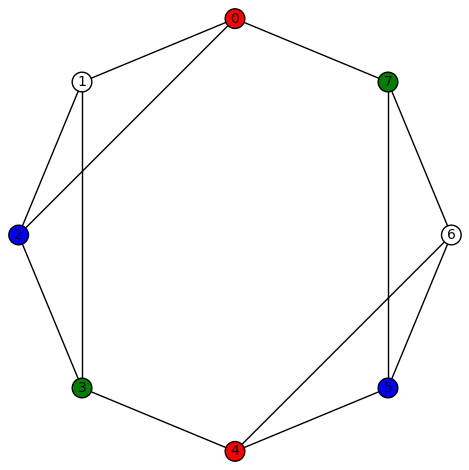
\includegraphics[height=5cm,width=5cm]{graphics/harmonic-quotient_d3reg8a-K4_30213201.png}
\end{center}
\begin{center}
%\vspace{8.0 cm}
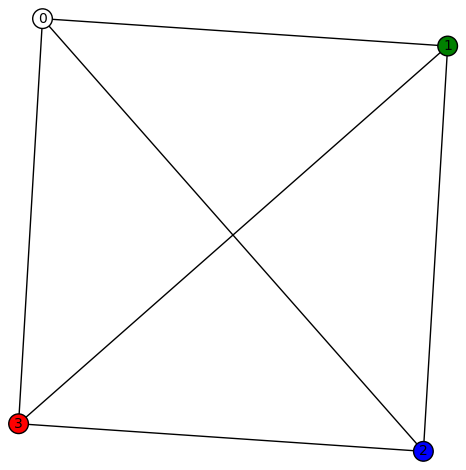
\includegraphics[height=4cm,width=4cm]{graphics/K4-0123b.png}
\end{center}
\end{minipage}
\caption{The cubic graph $\Gamma_2$, a degree two cover of $\Gamma_1=K_4$.}
\label{fig:harmonic-quotient_d3reg8a-K4_30213201}
\end{figure}

\begin{center}
\begin{tabular}{c|c|c|c}  
  $x$ & $\phi(x)$ & $m_\phi(x)$ & $\nu_\phi(x)$ \\ \hline
  0   &    3   &        1         &  0   \\ 
  1   &    0   &        1         &  0   \\ 
  2   &    2    &       1         &  0   \\ 
  3   &    1   &        1         &  0   \\ 
  4   &    3   &        1         &  0   \\ 
  5   &    2   &        1         &  0    \\ 
  6   &    0   &        1         &  0   \\ 
  7   &    1   &        1         &  0   \\ 
\end{tabular}
\end{center}
  
\[
  \genus(\Gamma_2) =5,\ \ \ \ \
  \genus(\Gamma_1) =3,
\]

\[
\deg(\phi) =2.
\]
Note that the vertex matrix map for the map $\phi:\Gamma_2\to \Gamma_1\cong K_4$ is given by

\[
\Phi =
\left(\begin{array}{rrrr}
0 & 0 & 0 & 1 \\
1 & 0 & 0 & 0 \\
0 & 0 & 1 & 0 \\
0 & 1 & 0 & 0 \\
0 & 0 & 0 & 1 \\
0 & 0 & 1 & 0 \\
1 & 0 & 0 & 0 \\
0 & 1 & 0 & 0
\end{array}\right).
\]
This matrix is invariant under the quotient group
$G = \langle (0,4)(1,6)(2,5)(3,7)\rangle$, regarded as
a row permutation of the matrix.

When $G=\langle (0,7)(1,5)(2,6)(3,4) \rangle$, then
$\Gamma_1=\Gamma_2/G$ is isomorphic to the diamond graph.
The harmonic quotient morphism is depicted in
Figure \ref{fig:harmonic-quotient_d3reg8a-diamond_02311230}
and tabulated below.

\begin{center}
\begin{tabular}{c|c|c|c}  
  $x$ & $\phi(x)$ & $m_\phi(x)$ & $\nu_\phi(x)$ \\ \hline
  0   &    0   &        1         &  1   \\ 
  1   &    2   &        1         &  0   \\ 
  2   &    3    &       1         &  0   \\ 
  3   &    1   &        1         &  1   \\ 
  4   &    1   &        1         &  1   \\ 
  5   &    2   &        1         &  0    \\ 
  6   &    3   &        1         &  0   \\ 
  7   &    0   &        1         &  1   \\ 
\end{tabular}
\end{center}

\[
  \genus(\Gamma_2) =5,\ \ \ \ \
  \genus(\Gamma_1) =2,
\]

\[
\deg(\phi) =2.
\]

\begin{figure}[H]
\begin{minipage}{\textwidth}
\begin{center}
%\vspace{8.0 cm}
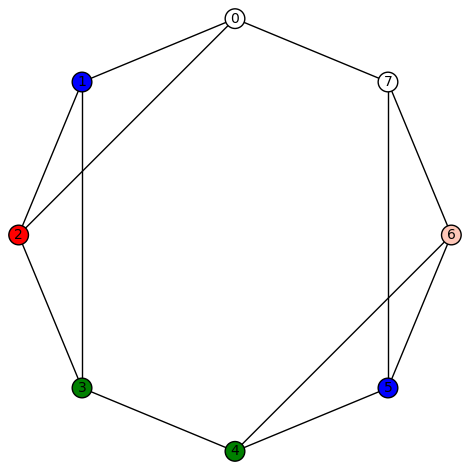
\includegraphics[height=5cm,width=5cm]{graphics/harmonic-quotient_d3reg8a-diamond_02311230.png}
\end{center}
\begin{center}
%\vspace{8.0 cm}
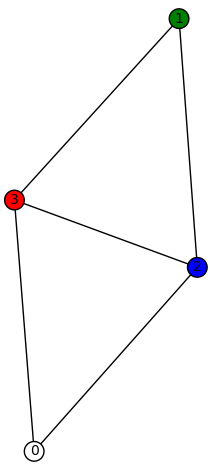
\includegraphics[height=5cm,width=3cm]{graphics/diamond_0123c.png}
\end{center}
\end{minipage}
\caption{The cubic graph  $\Gamma_2$ ({\tt d3reg8a}), a degree two quasicover of the diamond graph.}
\label{fig:harmonic-quotient_d3reg8a-diamond_02311230}
\end{figure}


Note that the diamond graph is a matchstick graph. The graph $K_4$ is not,
since the plane contains no four points at mutual distance $1$.

\begin{revremark}
\label{rem:matchstick}
The statements that {\tt d3reg8a} (this example) and
{\tt d4reg12e} (Example~\ref{example:d4reg12e}) are matchstick graphs were
not verified in 2026. Both graphs are planar, which is necessary. The
$3$-sun $S_3$ of Example~\ref{example:d4reg9a} is a matchstick graph. Draw
a unit equilateral triangle and attach a unit equilateral triangle to each
of its sides.
\end{revremark}
}
\end{example}



\begin{example}% d3reg8b
\label{example:d3reg8b}
    {\tt d3reg8b}\newline
{\rm  
Let $\Gamma_2$ have vertices

\[
V_2=\{0,1,\dots,7\}
\]
and edges

\[
E_2 = \{(0, 1), (0, 4), (0, 7), (1, 2), (1, 7), (2, 3), (2, 6),
\]
\[
(3, 4), (3, 5), (4, 5), (5, 6), (6, 7)\}.
\]
In this case, there are only $2$ harmonic quotient morphisms
$\pi: \Gamma_2\to \Gamma_2/G$, for some subgroup
$G$ of $\Aut(\Gamma_2)$. For $G=\Aut(\Gamma_2)$ (of order $4$) the quotient is
$P_3$, with fibers $\{0,4\}$, $\{1,3,5,7\}$, $\{2,6\}$.
When $G=\langle (0,4)(1,5)(2,6)(3,7)\rangle$, then
$\Gamma_1=\Gamma_2/G$ is isomorphic to the diamond graph.
The harmonic quotient morphism (a quasicover) is depicted in
Figure \ref{fig:harmonic-quotient_d3reg8b-diamond_21302130}
and tabulated below.

\begin{center}
\begin{tabular}{c|c|c|c}  
  $x$ & $\phi(x)$ & $m_\phi(x)$ & $\nu_\phi(x)$ \\ \hline
  0   &    2   &        1         &  1   \\
  1   &    1   &        1         &  0   \\
  2   &    3   &        1         &  1   \\
  3   &    0   &        1         &  0   \\
  4   &    2   &        1         &  1   \\
  5   &    1   &        1         &  0   \\
  6   &    3   &        1         &  1   \\
  7   &    0   &        1         &  0   \\
\end{tabular}
\end{center}

\[
  \genus(\Gamma_2) =5,\ \ \ \ \
  \genus(\Gamma_1) =2,
\]

\[
\deg(\phi) =2.
\]

\begin{figure}[H]
\begin{minipage}{\textwidth}
\begin{center}
%\vspace{8.0 cm}
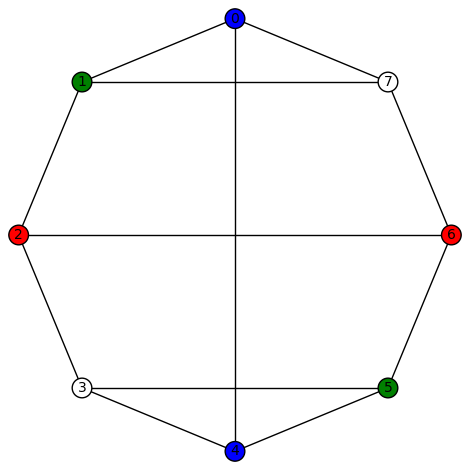
\includegraphics[height=5cm,width=5cm]{graphics/harmonic-quotient_d3reg8b-diamond_21302130.png}
\end{center}
\begin{center}
%\vspace{8.0 cm}
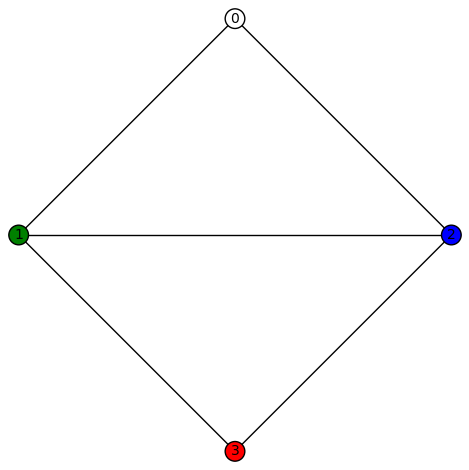
\includegraphics[height=5cm,width=4cm]{graphics/diamond-0123b.png}
\end{center}
\end{minipage}
\caption{The cubic graph  $\Gamma_2$ ({\tt d3reg8b}), a degree two quasicover of the diamond graph.}
\label{fig:harmonic-quotient_d3reg8b-diamond_21302130}
\end{figure}

}
\end{example}


\begin{example}% d3reg8c
\label{example:d3reg8c}
    {\tt d3reg8c}\newline
{\rm  
Let $\Gamma_2$ have vertices

\[
V_2=\{0,1,\dots,7\}
\]
and edges

\[
E_2 = \{
(0, 1), (0, 2), (0, 7), (1, 2), (1, 5), (2, 3), (3, 4),
\]
\[
(3, 6), (4, 5), (4, 7), (5, 6), (6, 7)
\}.
\]
In this case, there are only $2$ distinct
subgroups $G$ of $\Aut(\Gamma_2)$ with
harmonic quotient morphisms $\pi: \Gamma_2\to \Gamma_2/G$.
However, in both cases, $\Gamma_1=\Gamma_2/G$
is the same graph (isomorphic to the star graph $St_4$ on $4$ vertices)
and the morphisms are also the same.
\index{star graph}

When $G=\langle (0,2,1)(3,5,7) \rangle$, 
the harmonic quotient morphism is depicted in
Figure \ref{fig:harmonic-quotient_d3reg8c-star4_33302010}
and tabulated below.

\begin{center}
\begin{tabular}{c|c|c|c}  
  $x$ & $\phi(x)$ & $m_\phi(x)$ & $\nu_\phi(x)$ \\ \hline
  0   &    3   &        1         &  2   \\ 
  1   &    3   &        1         &  2   \\ 
  2   &    3    &       1         &  2   \\ 
  3   &    0   &        1         &  0   \\ 
  4   &    2   &        3         &  0   \\ 
  5   &    0   &        1         &  0    \\ 
  6   &    1   &        3         &  0   \\ 
  7   &    0   &        1         &  0   \\ 
\end{tabular}
\end{center}

\[
  \genus(\Gamma_2) =5,\ \ \ \ \
  \genus(\Gamma_1) =0,
\]

\[
\deg(\phi) =3.
\]

\begin{figure}[H]
\begin{minipage}{\textwidth}
\begin{center}
%\vspace{8.0 cm}
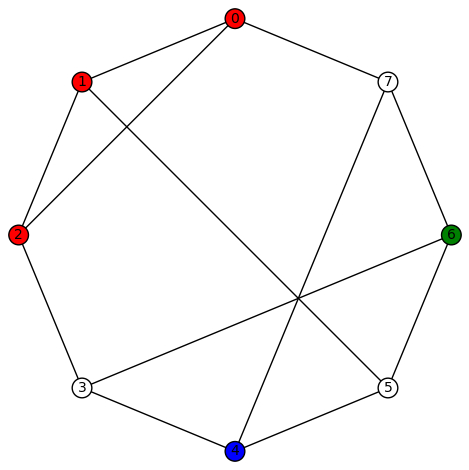
\includegraphics[height=5cm,width=5cm]{graphics/harmonic-quotient_d3reg8c-star4_33302010.png}
\end{center}
\begin{center}
%\vspace{8.0 cm}
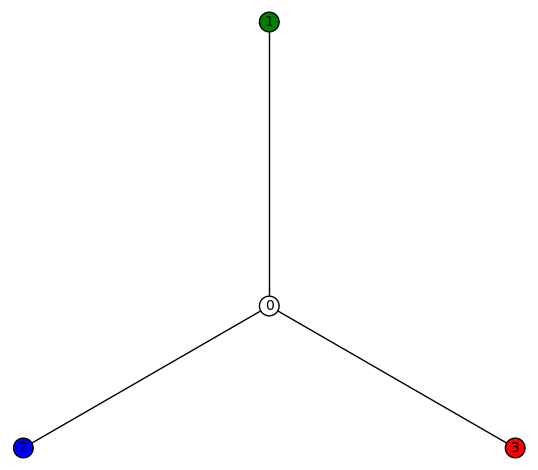
\includegraphics[height=5cm,width=4cm]{graphics/star4-0123.png}
\end{center}
\end{minipage}
\caption{The cubic graph  $\Gamma_2$ ({\tt d3reg8c}), a degree three harmonic quotient to the star graph, $St_4$.}
\label{fig:harmonic-quotient_d3reg8c-star4_33302010}
\end{figure}

When $G=\langle (1,2)(3,5), (0,2,1)(3,5,7) \rangle$
(a subgroup of order $6$),
the harmonic quotient morphism is the same as in
Figure \ref{fig:harmonic-quotient_d3reg8c-star4_33302010},
tabulated above.

}
\end{example}



\begin{example}% d3reg8d
\label{example:d3reg8d}
    {\tt d3reg8d}\newline
{\rm  
Let $\Gamma_2$ have vertices

\[
V_2=\{0,1,\dots,7\}
\]
and edges

\[
E_2 = \{(0, 1), (0, 5), (0, 7), (1, 2), (1, 4), (2, 3), (2, 7),
\]
\[
(3, 4), (3, 6), (4, 5), (5, 6), (6, 7)
\}.
\]
This graph has $55$ non-constant harmonic quotient
morphisms\footnote{These morphisms are distinct, unless indicated otherwise.}
$\pi: \Gamma_2\to \Gamma_2/G$, for some subgroup
$G$ of $\Aut(\Gamma_2)$. Of these, $3$ of these quotient graphs
are isomorphic to $C_4$, $6$ are isomorphic to the diamond graph,
$1$ is isomorphic to $K_4$,
$6$ are isomorphic to $P_3$, and the
remaining\footnote{Of these $39$, many are the same
morphism, even though the group $G$ is different, so there are
really only $11$ distinct harmonic quotient morphisms to $P_2$.}
$39$ are $P_2$. 

When $G=\langle (0,3)(1,6)(2,5)(4,7) \rangle$, 
the harmonic quotient morphism is depicted in
Figure \ref{fig:harmonic-quotient_d3reg8d-K4_30132102}
and tabulated below.

\begin{center}
\begin{tabular}{c|c|c|c}  
  $x$ & $\phi(x)$ & $m_\phi(x)$ & $\nu_\phi(x)$ \\ \hline
  0   &    3   &        1         &  0   \\ 
  1   &    0   &        1         &  0   \\ 
  2   &    1    &       1         &  0   \\ 
  3   &    3   &        1         &  0   \\ 
  4   &    2   &        1         &  0   \\ 
  5   &    1   &        1         &  0    \\ 
  6   &    0   &        1         &  0   \\ 
  7   &    2   &        1         &  0   \\ 
\end{tabular}
\end{center}

\[
  \genus(\Gamma_2) =5,\ \ \ \ \
  \genus(\Gamma_1) =3,
\]

\[
\deg(\phi) =2.
\]

\begin{figure}[H]
\begin{minipage}{\textwidth}
\begin{center}
%\vspace{8.0 cm}
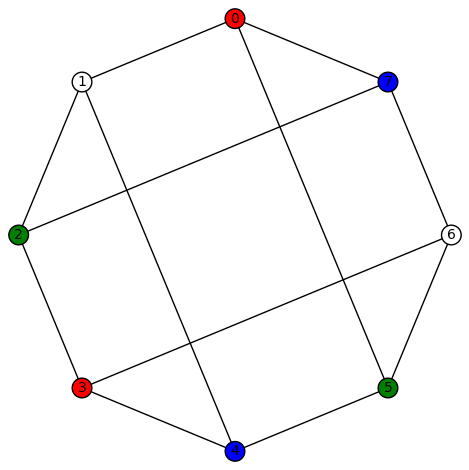
\includegraphics[height=5cm,width=5cm]{graphics/harmonic-quotient_d3reg8d-K4_30132102.png}
\end{center}
\begin{center}
%\vspace{8.0 cm}
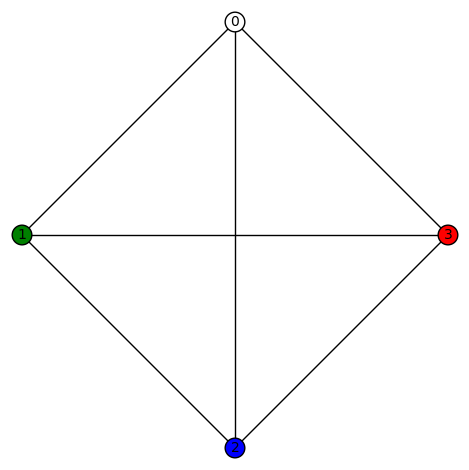
\includegraphics[height=5cm,width=4cm]{graphics/K4-0123.png}
\end{center}
\end{minipage}
\caption{The $3$-dimensional cube graph  $\Gamma_2$ ({\tt d3reg8d}), with a degree two harmonic quotient morphism (a covering) to the complete graph, $K_4$.}
\label{fig:harmonic-quotient_d3reg8d-K4_30132102}
\end{figure}

When $G=\langle (0,1)(2,7)(3,6)(4,5) \rangle$,
the harmonic quotient morphism (a quasicover) is depicted in
Figure \ref{fig:harmonic-quotient_d3reg8d-C4_11320023} and
tabulated below.

\begin{center}
\begin{tabular}{c|c|c|c}  
  $x$ & $\phi(x)$ & $m_\phi(x)$ & $\nu_\phi(x)$ \\ \hline
  0   &    1   &        1         &  1   \\ 
  1   &    1   &        1         &  1   \\ 
  2   &    3   &        1         &  1   \\ 
  3   &    2   &        1         &  1   \\ 
  4   &    0   &        1         &  1   \\ 
  5   &    0   &        1         &  1    \\ 
  6   &    2   &        1         &  1   \\ 
  7   &    3   &        1         &  1   \\ 
\end{tabular}
\end{center}

\[
  \genus(\Gamma_2) =5,\ \ \ \ \
  \genus(\Gamma_1) =1,
\]

\[
\deg(\phi) =2.
\]


\begin{figure}[H]
\begin{minipage}{\textwidth}
\begin{center}
%\vspace{8.0 cm}
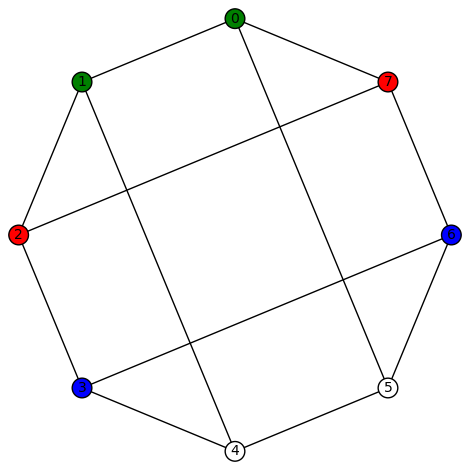
\includegraphics[height=5cm,width=5cm]{graphics/harmonic-quotient_d3reg8d-C4_11320023.png}
\end{center}
\begin{center}
%\vspace{8.0 cm}
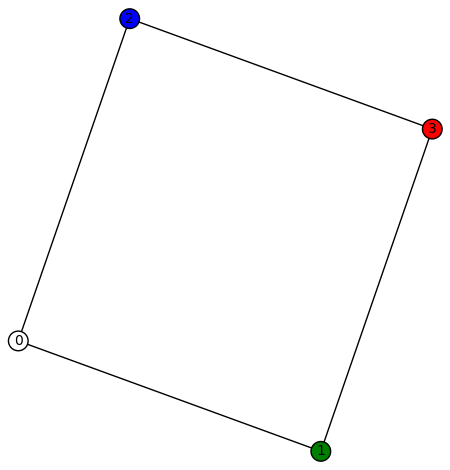
\includegraphics[height=5cm,width=4cm]{graphics/cycle4-0123b.png}
\end{center}
\end{minipage}
\caption{The cube graph  $\Gamma_2$ ({\tt d3reg8d}), with a degree two harmonic quotient morphism (a quasicovering) to the cycle graph, $C_4$.}
\label{fig:harmonic-quotient_d3reg8d-C4_11320023}
\end{figure}

}
\end{example}



\begin{example}% d3reg8e
\label{example:d3reg8e}
    {\tt d3reg8e}\newline
{\rm  
Let $\Gamma_2$ have vertices

\[
V_2=\{0,1,\dots,7\}
\]
and edges

\[
E_2 = \{(0, 1), (0, 4), (0, 7), (1, 2), (1, 6), (2, 3),
\]
\[
(2, 5), (3, 4), (3, 7), (4, 5), (5, 6), (6, 7)
\}.
\]
This Wagner graph has $7$ non-constant harmonic quotient
morphisms\footnote{These morphisms are distinct, unless indicated otherwise.}
$\pi: \Gamma_2\to \Gamma_2/G$, for some subgroup
$G$ of $\Aut(\Gamma_2)$. Of these quotient graphs,
$1$ is isomorphic to $C_4$, $2$ are isomorphic to $P_3$, and
$4$ are\footnote{Of these $4$, two are the same
morphism, even though the group $G$ is different, so there are
really only $3$ distinct harmonic quotient morphisms to $P_2$.}
isomorphic to $P_2$.

When $G=\langle (0,7)(1,6)(2,5)(3,4) \rangle$,
the harmonic quotient morphism (a quasicover) is depicted in
Figure \ref{fig:harmonic-quotient_d3reg8e-C4_03211230} and
tabulated below.

\begin{center}
\begin{tabular}{c|c|c|c}  
  $x$ & $\phi(x)$ & $m_\phi(x)$ & $\nu_\phi(x)$ \\ \hline
  0   &    0   &        1         &  1   \\
  1   &    3   &        1         &  1   \\
  2   &    2   &        1         &  1   \\
  3   &    1   &        1         &  1   \\
  4   &    1   &        1         &  1   \\
  5   &    2   &        1         &  1   \\
  6   &    3   &        1         &  1   \\
  7   &    0   &        1         &  1   \\
\end{tabular}
\end{center}

\[
  \genus(\Gamma_2) =5,\ \ \ \ \
  \genus(\Gamma_1) =1,
\]

\[
\deg(\phi) =2.
\]


\begin{figure}[H]
\begin{minipage}{\textwidth}
\begin{center}
%\vspace{8.0 cm}
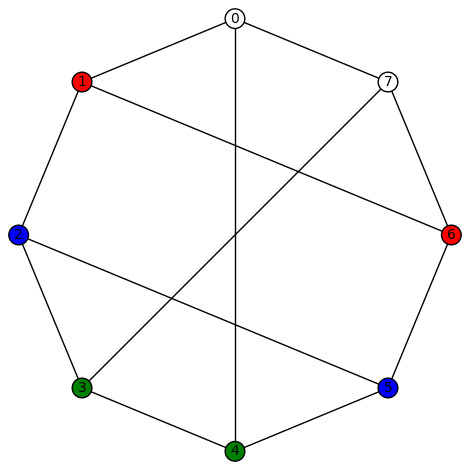
\includegraphics[height=5cm,width=5cm]{graphics/harmonic-quotient_d3reg8e-C4_03211230.png}
\end{center}
\begin{center}
%\vspace{8.0 cm}
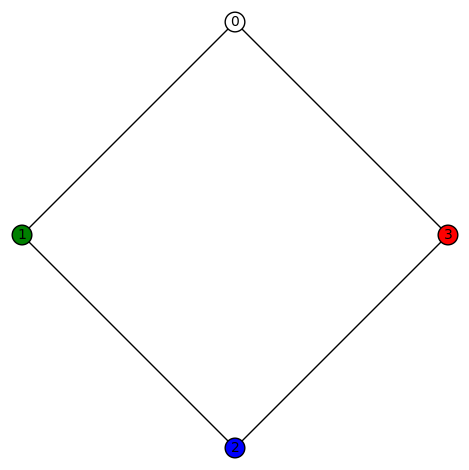
\includegraphics[height=5cm,width=4cm]{graphics/Cycle4-0123.png}
\end{center}
\end{minipage}
\caption{The cubic graph  $\Gamma_2$ ({\tt d3reg8e}), with a degree two harmonic quotient morphism (a quasicovering) to the cycle graph, $C_4$.}
\label{fig:harmonic-quotient_d3reg8e-C4_03211230}
\end{figure}

}
\end{example}






\subsection{\texorpdfstring{$10$}{10} vertices}

This subsection describes the connected cubic graphs on $10$ vertices.
It records their invariants and harmonic morphism counts, and then
works out harmonic quotient morphisms in examples.

%%% file-of-3regular10-graphs.txt
\label{subsec:d3reg10}

There are 19 $3$-regular graphs with $10$ vertices.
Three of these cubic graphs are vertex transitive and one of these
three (namely, the Petersen graph) is also edge transitive.
All but two of these graphs are Hamiltonian (circumference $|V|=10$).
One of these two has a bridge (the first one listed below)
and circumference $5$.
The other one of these two non-Hamiltonian graphs,
the Petersen graph, has circumference $9$.

{\small{
\begin{center}
\begin{tabular}{c|c|c|c|c}
  graph label & LCF & $|\Aut(\Gamma)|$ & genus & $|K(\Gamma)|$ \\ \hline
  d3reg10a & -- & 32 & 6 & $576=2^63^2$ \\
  d3reg10b & (10, [4,2,3,-2,-4,-3,2,2,-2,-2], 1) & 4 & 6 & $1160=2^35\cdot 29$ \\
  d3reg10c & (10, [2,-3,-2,2,2,-2,-2,2,3,-2], 1) & 8 & 6 & $1080=2^33^35$ \\
  d3reg10d & (10, [-2,-2,3,3,3,-3,-3,-3,2,2], 1) & 16 & 6 & $1224=2^33^217$ \\ 
  d3reg10e & (10, [2,2,-2,-2,5], 2) & 16 & 6 & $960=2^63\cdot 5$ \\
  d3reg10f & (10, [2,3,-2,5,-3], 2) & 2 & 6 & $1488=2^43\cdot 31$ \\  
  d3reg10g & (10, [2,-4,-2,5,2,4,-2,4,5,-4], 1) & 12 & 6 & $1600=2^65^2$ \\  
  d3reg10h & (10, [5,3,5,-4,-3,5,2,5,-2,4], 1) & 2 & 6 & $1717=17\cdot 101$ \\  
  d3reg10i & (10, [-4,3,3,5,-3,-3,4,2,5,-2], 1) & 4 & 6 & $1599=3\cdot 13\cdot 41$ \\  
  d3reg10j & (10, [3,-3,5,-3,2,4,-2,5,3,-4], 1) & 6 & 6 & $1682 = 2\cdot 29^2$ \\  
  d3reg10k & (10, [-4, 4, 2, 5, -2], 2) & 4 & 6 & $1463=7\cdot 11\cdot 19$ \\  
  d3reg10l & (10, [5,-2,2,4,-2,5,2,-4,-2,2], 1) & 6 & 6 & $1445= 5\cdot 17^2$ \\  
  d3reg10m & (10, [2,5,-2,5,5], 2) & 8 & 6 & $1573=11^213$ \\
  d3reg10n & (10, [5,-3,-3,3,3], 2) & 48 & 6 & $1728 = 2^6 3^3$ \\    
  d3reg10o & (10, [5,-4,4,-4,4], 2) & 8  & 6 & $1920=2^7 3\cdot 5$ \\    
  d3reg10p & (10, [5,-4,4,5,5], 2) & 4  & 6 & $1881=3^2 11\cdot 19$ \\    
  d3reg10q & (10, [5,5,-3,5,3], 2)  & 20  & 6 & $1815=3\cdot 5\cdot 11^2$ \\    
  d3reg10r & (10,[-4, 4, -3, 5, 3],2) & 20  & 6 & $1805=5\cdot 19^2$ \\    
  d3reg10s & --  & 120  & 6 & $2000=2^45^3$ \\    
\end{tabular}
\end{center}  
}}

\begin{enumerate}
\item
  {\tt d3reg10a}\newline
The one with vertices and edges:

\[
V=\{ 0, 1, 2, 3, 4, 5, 6, 7, 8, 9\},
\]
\[
E = \{ (0, 1), (0, 6), (0, 9), (1, 2), (1, 5), (2, 3), (2, 4), (3, 4),
\]
\[
(3, 5), (4, 5), (6, 7), (6, 8), (7, 8), (7, 9), (8, 9)\}.
\]
It has %automorphism group of order $32$,
characteristic polynomial  
\[
x^{10} - 15x^8 - 8x^7 + 63x^6 + 64x^5 - 37x^4 - 56x^3 - 12x^2,
\]
Diameter $5$,
girth $3$,
circumference $5$.
This is not Hamiltonian (indeed, it has a bridge).
%It has critical group of cardinality $576=2^63^2$.

It has $8$ non-trivial harmonic morphisms to $P_3$, but
no non-trivial harmonic morphisms to $P_4$, $St_4$, $C_3$, $C_4$, or to $K_4$.


\item
  {\tt d3reg10b}\newline
The one with characteristic polynomial  
\[
x^{10} - 15x^8 - 6x^7 + 69x^6 + 48x^5 - 96x^4 - 76x^3 + 30x^2 + 26x + 3
\]
Diameter $4$,
girth $3$,
circumference $10$.
This is a Hamiltonian graph.
%It has critical group of cardinality $1160=2^35\cdot 29$.

This particular graph is very unusual in that it lacks non-trivial
harmonic morphisms to all ``very small'' graphs.
It has no non-trivial harmonic morphisms to the diamond graph,
$St_4$, $P_3$, (hence none to $P_4$, $P_5$, \dots),
%by Lemma \ref{lemma:families}),
$C_3$, $C_4$, or to $K_4$.

SageMath command:

\verb@graphs.LCFGraph(10, [4, 2, 3, -2, -4, -3, 2, 2, -2, -2], 1)@


\item
  {\tt d3reg10c}\newline
The one with %automorphism group of order $8$ and having
characteristic polynomial  
\[
x^{10} - 15x^8 - 8x^7 + 71x^6 + 68x^5 - 93x^4 - 132x^3 - 36x^2 
\]
Diameter $3$,
girth $3$,
circumference $10$.
This is a Hamiltonian graph.% (with circumference $10$).
%It has critical group of cardinality $1080=2^33^35$.

It has $8$ non-trivial harmonic morphisms to $P_3$,
$6$ non-trivial harmonic morphisms to $C_3$,
but no non-trivial harmonic morphisms to the diamond graph,
$St_4$, $P_4$, $C_4$, or to $K_4$.

SageMath command:

\verb@graphs.LCFGraph(10, [2, -3, -2, 2, 2, -2, -2, 2, 3, -2], 1)@


\item
  {\tt d3reg10d}\newline
The one with %automorphism group of order $16$ and having
characteristic polynomial  
\[
x^{10} - 15x^8 - 4x^7 + 63x^6 + 36x^5 - 61x^4 - 56x^3 - 12x^2 
\]
Diameter $3$,
girth $3$,
circumference $10$.
This is a Hamiltonian graph.
%It has critical group of cardinality $1224=2^33^217$.

It has $12$ non-trivial harmonic morphisms to $St_4$,
$12$ non-trivial harmonic morphisms to $P_3$,
$12$ non-trivial harmonic morphisms to $C_3$,
but no non-trivial harmonic morphisms to the diamond graph,
$P_4$, $C_4$, or to $K_4$.

SageMath command:

\verb@graphs.LCFGraph(10, [-2, -2, 3, 3, 3, -3, -3, -3, 2, 2], 1)@


\item
  {\tt d3reg10e}\newline
The one with %automorphism group of order $16$ and having
characteristic polynomial  

\[
x^{10} - 15x^8 - 8x^7 + 71x^6 + 64x^5 - 101x^4 - 104x^3 + 44x^2 + 48x 
\]
Diameter $4$,
girth $3$,
circumference $10$.
This is a Hamiltonian graph.% (with circumference $10$).
%It has critical group of cardinality $960=2^63\cdot 5$.

It has $4$ non-trivial harmonic morphisms to $P_3$,
but no non-trivial harmonic morphisms to $St_4$, $P_4$, $C_3$, $C_4$,
or to $K_4$.

SageMath command:

\verb@graphs.LCFGraph(10,[2,2,-2,-2,5],2)@


\item
  {\tt d3reg10f}\newline
The one with %automorphism group of order $2$ and having
characteristic polynomial  

\[
x^{10} - 15x^8 - 4x^7 + 71x^6 + 28x^5 - 121x^4 - 48x^3 + 64x^2 + 24x 
\]
Diameter $3$,
girth $3$,
circumference $10$.
This is a Hamiltonian graph.
%It has critical group of cardinality $1488=2^43\cdot 31$.

It has $2$ non-trivial harmonic morphisms to $P_3$,
but no non-trivial harmonic morphisms to $St_4$, $P_4$, $C_3$, $C_4$, or to
$K_4$.

SageMath command:

\verb@graphs.LCFGraph(10,[2,3,-2,5,-3],2)@


\item
  {\tt d3reg10g}\newline
The one with %automorphism group of order $12$ and having
characteristic polynomial  

\[
x^{10} - 15x^8 - 4x^7 + 75x^6 + 24x^5 - 157x^4 - 36x^3 + 144x^2 + 16x - 48
\]
Diameter $3$,
girth $3$,
circumference $10$.
This is a Hamiltonian graph.
%It has critical group of cardinality $1600=2^65^2$.

It has $6$ non-trivial harmonic morphisms to $St_4$,
$6$ non-trivial harmonic morphisms to $P_3$, but
no non-trivial harmonic morphisms to $P_4$, $C_3$, $C_4$, or to $K_4$.

SageMath command:

\verb@graphs.LCFGraph(10, [2, -4, -2, 5, 2, 4, -2, 4, 5, -4], 1)@


\item
  {\tt d3reg10h}\newline
The one with %automorphism group of order $2$ and having
characteristic polynomial  

\[
x^{10} - 15x^8 - 2x^7 + 71x^6 + 8x^5 - 132x^4 - 2x^3 + 91x^2 - 8x - 12
\]
Diameter $3$,
girth $3$,
circumference $10$.
This is a Hamiltonian graph.
%This has critical group of order $1717=17\cdot 101$.

It has $2$ non-trivial harmonic morphisms to $P_3$, but
no non-trivial harmonic morphisms to $St_4$, $P_4$,
$C_3$, $C_4$, or to $K_4$.

SageMath command:

\verb@graphs.LCFGraph(10,[5, 3, 5, -4, -3, 5, 2, 5, -2, 4], 1)@


\item
  {\tt d3reg10i}\newline
The one with %automorphism group of order $4$ and having
characteristic polynomial  

\[
x^{10} - 15x^8 - 2x^7 + 67x^6 + 12x^5 - 96x^4 - 22x^3 + 35x^2 + 12x 
\]
Diameter $3$,
girth $3$,
circumference $10$.
This is a Hamiltonian graph.% (with circumference $10$).
%This has critical group of order $1599=3\cdot 13\cdot 41$.

It has $6$ non-trivial harmonic morphisms to $St_4$,
$6$ non-trivial harmonic morphisms to $P_3$,
but
no non-trivial harmonic morphisms to $P_4$, $C_3$, $C_4$, or to $K_4$.

SageMath command:

\verb@graphs.LCFGraph(10,[-4, 3, 3, 5, -3, -3, 4, 2, 5, -2],1)@


\item
  {\tt d3reg10j}\newline
The one with %automorphism group of order $6$ and having
characteristic polynomial  

\[
x^{10} - 15x^8 - 2x^7 + 69x^6 + 12x^5 - 116x^4 - 24x^3 + 54x^2 + 26x + 3 
\]
Diameter $3$,
girth $3$,
circumference $10$.
%has girth $3$ and diameter $3$.
This is a Hamiltonian graph.% (with circumference $10$).
%This has critical group of order $1682 = 2\cdot 29^2$.

It has $6$ non-trivial harmonic morphisms to $P_3$, but
no non-trivial harmonic morphisms to
$St_4$, $P_4$, $C_3$, $C_4$, or to $K_4$.

SageMath command:

\verb@graphs.LCFGraph(10,[3, -3, 5, -3, 2, 4, -2, 5, 3, -4], 1)@


\item
  {\tt d3reg10k}\newline
The one with %automorphism group of order $4$ and having
characteristic polynomial  

\[
x^{10} - 15x^8 - 4x^7 + 69x^6 + 32x^5 - 105x^4 - 64x^3 + 23x^2 + 20x + 3 
\]
Diameter $3$,
girth $3$,
circumference $10$.
This is a Hamiltonian graph.% (with circumference $10$).
This has critical group of order $1463=7\cdot 11\cdot 19$.

It has $6$ non-trivial harmonic morphisms to $P_3$, but
no non-trivial harmonic morphisms to $St_4$,
$P_4$, $C_3$, $C_4$, or to $K_4$.

SageMath command:

\verb@graphs.LCFGraph(10,[-4, 4, 2, 5, -2], 2)@


\item
  {\tt d3reg10l}\newline
The one with %automorphism group of order $6$ and having
characteristic polynomial  

\[
x^{10} - 15x^8 - 6x^7 + 75x^6 + 48x^5 - 144x^4 - 114x^3 + 75x^2 + 68x + 12 
\]
Diameter $3$,
girth $3$,
circumference $10$.
This is a Hamiltonian graph.
%This has critical group of order $1445= 5\cdot 17^2$.

It has no non-trivial harmonic morphisms to $St_4$, $P_4$, $C_3$, $C_4$,
or to $K_4$. However, it has $6$ non-trivial harmonic morphisms to $P_3$.

SageMath command:

\verb@graphs.LCFGraph(10, [5, -2, 2, 4, -2, 5, 2, -4, -2, 2], 1)@


\item
  {\tt d3reg10m}\newline
The one with %automorphism group of order $8$ and having
characteristic polynomial  

\[
x^{10} - 15x^8 - 4x^7 + 73x^6 + 28x^5 - 141x^4 - 52x^3 + 99x^2 + 16x - 21 
\]
Diameter $3$,
girth $3$,
circumference $10$.
This is a Hamiltonian graph.% (with circumference $10$).
%This has critical group of order $1573=11^213$.

It has $2$ non-trivial harmonic morphisms to $P_3$, but
no non-trivial harmonic morphisms to $St_4$, $P_4$, $C_4$, or to $K_4$.

SageMath command:

\verb@graphs.LCFGraph(10,[2, 5, -2, 5, 5],2)@


\item
  {\tt d3reg10n}\newline
The one with %automorphism group of order $48$ and having
characteristic polynomial  

\[
x^{10} - 15x^8 + 63x^6 - 85x^4 + 36x^2  
\]
Diameter $3$,
girth $4$,
circumference $10$.
This is an integral\footnote{Its adjacency matrix has
  eigenvalues $3, 2, 1, 1, 0, 0, -1, -1, -2, -3$, while
  (since the graph is cubic) its Laplacian has eigenvalues
  $6, 5, 4, 4, 3, 3, 2, 2, 1, 0$.},
Hamiltonian graph.
%This has critical group of cardinality $1728 = 2^6 3^3$.

It has $18$ non-trivial harmonic morphisms to $St_4$,
$22$ non-trivial harmonic morphisms to $P_3$,
$8$ non-trivial harmonic morphisms to $P_4$,
but no non-trivial harmonic morphisms to $C_3$, $C_4$ or $K_4$.
By a computer check using SageMath , we know there
are no non-trivial harmonic morphisms to $P_5$.
%More generally, using Theorem \ref{thrm:diameter-bound}
Therefore, we know there
are no non-trivial harmonic morphisms to $P_k$, for $k\geq 5$.
\index{integral graph}

SageMath command:

\verb@graphs.LCFGraph(10, [5, -3, -3, 3, 3], 2)@


\item
  {\tt d3reg10o}\newline
The one with %automorphism group of order $8$ and having
characteristic polynomial  

\[
x^{10} - 15x^8 + 71x^6 - 16x^5 - 133x^4 + 64x^3 + 76x^2 - 48x  
\]
Diameter $3$,
girth $4$,
circumference $10$.
This is a Hamiltonian graph.
%The critical group has cardinality $1920=2^7 3\cdot 5$.

It has $6$ non-trivial harmonic morphisms to $St_4$,
$8$ non-trivial harmonic morphisms to $P_3$,
but no non-trivial harmonic morphisms to $P_4$, $C_3$, $C_4$, or to $K_4$.

SageMath command:

\verb@graphs.LCFGraph(10,[5, -4, 4, -4, 4],2)@


\item
  {\tt d3reg10p}\newline
The one with %automorphism group of order $4$ and having
characteristic polynomial  

\[
x^{10} - 15x^8 + 69x^6 -12x^5 - 117x^4 +36x^3 + 59x^2 -12x - 9  
\]
Diameter $3$,
girth $4$,
circumference $10$.
This is a Hamiltonian graph.% (with circumference $10$).
%This has critical group of order $1881=3^2 11\cdot 19$.

It has $2$ non-trivial harmonic morphisms to $P_3$,
but no non-trivial harmonic morphisms to $St_4$, $P_4$,
$C_3$, $C_4$, or to $K_4$.


SageMath command:

\verb@graphs.LCFGraph(10,[5, -4, 4, 5, 5],2)@


\item
  {\tt d3reg10q}\newline
The one with %automorphism group of order $20$ (acting transitively on the vertices of the graph) and having
characteristic polynomial  

\[
x^{10} - 15x^8 + 65x^6 - 105x^4 + 55x^2 - 9  
\]
Diameter $3$,
girth $4$,
circumference $10$.
This graph is vertex transitive, not edge transitive, but it is
Hamiltonian.% (with circumference $10$).
This has critical group of order $1815=3\cdot 5\cdot 11^2$.

It has $10$ non-trivial harmonic morphisms to $P_3$,
but no non-trivial harmonic morphisms to $St_4$, $P_4$, $C_3$,
$C_4$, or to $K_4$.

SageMath command:

\verb@graphs.LCFGraph(10,[5, 5, -3, 5, 3],2)@


\item
  {\tt d3reg10r}\newline
The one with %automorphism group of order $20$ (acting transitively on the vertices of the graph) and having
characteristic polynomial  

\[
x^{10} - 15x^8 + 65x^6 - 4x^5 - 85x^4 - 20x^3 + 35x^2 + 20x + 3
\]
Diameter $3$,
girth $4$,
circumference $10$.
This graph is vertex transitive, not edge transitive,
but it is Hamiltonian.% (with circumference $10$).
%This has critical group of order $1805=5\cdot 19^2$.

It has $10$ non-trivial harmonic morphisms to $P_3$,
but no non-trivial harmonic morphisms to $St_4$, $P_4$, $C_3$, $C_4$,
or to $K_4$.


SageMath command:

\verb@graphs.LCFGraph(10,[-4, 4, -3, 5, 3],2)@


\item
  {\tt d3reg10s}
  The Petersen graph with vertices and edges:

\[
V=\{ 0,1,2,3,4,5,6,7,8,9\},
\]
\[
E = \{ (0, 1), (0, 4), (0, 5), (1, 2), (1, 6), (2, 3), (2, 7), (3, 4), (3, 8),
\]
\[
(4, 9), (5, 7), (5, 8), (6, 8), (6, 9), (7, 9) \}.
\]
The automorphism group acts transitively
on the vertices {\it and} the edges of the graph. It has
characteristic polynomial  
\index{Petersen graph}

\[
x^{10} - 15x^8 + 75x^6 - 24x^5 - 165x^4 + 120x^3 + 120x^2 - 160x +48,
\]
Diameter $2$,
girth $5$,
circumference $9$.
It is symmetric (arc transitive),
distance regular, integral, and is strongly regular with
parameters $(10,3,0,1)$.
This is {\it not} a Hamiltonian graph, but has circumference $9$.
%This has critical group of order $2000=2^45^3$.
\index{integral graph}

It has $30$ non-trivial harmonic morphisms to $St_4$ and
$30$ non-trivial harmonic morphisms to $P_3$.
However, it has
no non-trivial harmonic morphisms to $P_4$, $C_3$, $C_4$, or to $K_4$.

\end{enumerate}  



\subsubsection{Examples}
\label{sec:d3reg10-examples}

Each example below takes one graph from the list above and describes
its harmonic quotient morphisms.


\begin{example}% d3reg10a
\label{example:d3reg10a}
  {\tt d3reg10a}\newline
{\rm  
Let $\Gamma_2$ have vertices

\[
V_2=\{0,1,\dots,9\}
\]
and edges

\[
E_2 = \{
(0, 1), (0, 6), (0, 9), (1, 2), (1, 5), (2, 3), (2, 4), (3, 4),
\]
\[
(3, 5), (4, 5), (6, 7), (6, 8), (7, 8), (7, 9), (8, 9)
\}.
\]
This graph has $4$ distinct non-constant harmonic quotient
morphisms $\pi: \Gamma_2\to \Gamma_2/G$, for some subgroup
$G$ of $\Aut(\Gamma_2)$. All quotients are isomorphic to the
graph\footnote{This graph is basically the wheel graph
with $4$ ``rim'' vertices, but remove one of the ``spoke'' edges.
}
$\Gamma_1$ have vertices

\[
V_1=\{0,1,\dots,4\}
\]
and edges

\[
E_1 = \{
(0, 1), (0, 3), (0, 4), (1, 2), (1, 4), (2, 3), (3, 4)
\}.
\]
One of these quotient morphisms is tabulated below.
\begin{center}
\begin{tabular}{c|c|c|c}  
  $x$ & $\phi(x)$ & $m_\phi(x)$ & $\nu_\phi(x)$ \\ \hline
  0   &    2   &        1         &  1   \\ 
  1   &    2   &        1         &  1   \\ 
  2   &    3   &        1         &  0   \\ 
  3   &    0   &        1         &  0   \\ 
  4   &    4   &        1         &  0   \\ 
  5   &    1   &        1         &  0    \\ 
  6   &    1   &        1         &  0   \\ 
  7   &    4   &        1         &  0   \\
  8   &    0   &        1         &  0   \\
  9   &    3   &        1         &  0   \\ 
\end{tabular}
\end{center}

\[
  \genus(\Gamma_2) =6,\ \ \ \ \
  \genus(\Gamma_1) =3,
\]

\[
\deg(\phi) =2.
\]

}
\end{example}


\begin{example}% d3reg10b
\label{example:d3reg10b}
  {\tt d3reg10b}\newline
{\rm  
Let $\Gamma_2$ have vertices

\[
V_2=\{0,1,\dots,9\}
\]
and edges

\[
E_2 = \{
(0, 1), (0, 4), (0, 9), (1, 2), (1, 3), (2, 3), (2, 5), (3, 4),
\]
\[
(4, 5), (5, 6), (6, 7), (6, 8), (7, 8), (7, 9), (8, 9)
\}.
\]
This graph has no non-constant harmonic quotient
morphisms $\pi: \Gamma_2\to \Gamma_2/G$, for some subgroup
$G$ of $\Aut(\Gamma_2)$.

}
\end{example}


\begin{example}% d3reg10c
\label{example:d3reg10c}
  {\tt d3reg10c}\newline
{\rm  
Let $\Gamma_2$ have vertices

\[
V_2=\{0,1,\dots,9\}
\]
and edges

\[
E_2 = \{
(0, 1), (0, 2), (0, 9), (1, 2), (1, 8), (2, 3), (3, 4), (3, 5),
\]
\[
(4, 5), (4, 6), (5, 6), (6, 7), (7, 8), (7, 9), (8, 9)
\}.
\]
This graph has no non-constant harmonic quotient
morphisms $\pi: \Gamma_2\to \Gamma_2/G$, for some subgroup
$G$ of $\Aut(\Gamma_2)$.

}
\end{example}

\begin{example}% d3reg10d
\label{example:d3reg10d}
  {\tt d3reg10d}\newline
{\rm  
Let $\Gamma_2$ have vertices

\[
V_2=\{0,1,\dots,9\}
\]
and edges

\[
E_2 = \{
(0, 1), (0, 8), (0, 9), (1, 2), (1, 9), (2, 3), (2, 5), (3, 4),
\]
\[
(3, 6), (4, 5), (4, 7), (5, 6), (6, 7), (7, 8), (8, 9)
\}.
\]
This graph has no non-constant harmonic quotient
morphisms $\pi: \Gamma_2\to \Gamma_2/G$, for some subgroup
$G$ of $\Aut(\Gamma_2)$.

}
\end{example}

\begin{example}% d3reg10e
\label{example:d3reg10e}
  {\tt d3reg10e}\newline
{\rm  
Let $\Gamma_2$ have vertices

\[
V_2=\{0,1,\dots,9\}
\]
and edges

\[
E_2 = \{
(0, 1), (0, 2), (0, 9), (1, 2), (1, 3), (2, 3), (3, 4), (4, 5),
\]
\[
(4, 9), (5, 6), (5, 7), (6, 7), (6, 8), (7, 8), (8, 9)
\}.
\]
This graph has $2$ distinct non-constant harmonic quotient
morphisms $\pi: \Gamma_2\to \Gamma_2/G$, for some subgroup
$G$ of $\Aut(\Gamma_2)$. All quotients are isomorphic to the
graph $\Gamma_1$ having vertices

\[
V_1=\{0,1,\dots,4\}
\]
and edges

\[
E_1 = \{
(0, 1), (0, 2), (0, 3), (1, 2), (1, 4), (2, 4), (3, 4)
\}.
\]
One of these quotient morphisms is tabulated below.
\begin{center}
\begin{tabular}{c|c|c|c}  
  $x$ & $\phi(x)$ & $m_\phi(x)$ & $\nu_\phi(x)$ \\ \hline
  0   &    4   &        1         &  0   \\ 
  1   &    1   &        1         &  0   \\ 
  2   &    2   &        1         &  0   \\ 
  3   &    0   &        1         &  0   \\ 
  4   &    3   &        1         &  1   \\ 
  5   &    4   &        1         &  0    \\ 
  6   &    2   &        1         &  0   \\ 
  7   &    1   &        1         &  0   \\
  8   &    0   &        1         &  0   \\
  9   &    3   &        1         &  1   \\ 
\end{tabular}
\end{center}

\[
  \genus(\Gamma_2) =6,\ \ \ \ \
  \genus(\Gamma_1) =3,
\]

\[
\deg(\phi) =2.
\]
The uncolored graphs are depicted in Figure \ref{fig:harmonic-quotient_d3reg10e-Gamma1}.

\begin{figure}[H]
\begin{minipage}{\textwidth}
\begin{center}
%\vspace{8.0 cm}
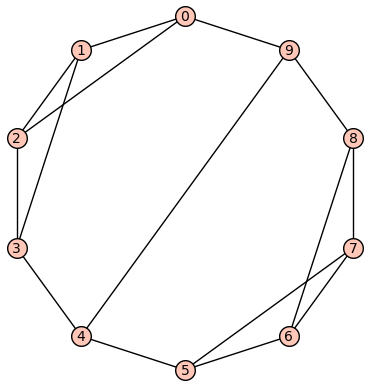
\includegraphics[height=5cm,width=5cm]{graphics/graph_d3reg10e.png}
\end{center}
\begin{center}
%\vspace{8.0 cm}
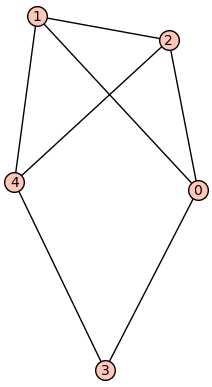
\includegraphics[height=4cm,width=4cm]{graphics/C4-C3-C3.png}
\end{center}
\end{minipage}
\caption{The cubic graph  $\Gamma_2$ ({\tt d3reg10e}), with a degree two harmonic quotient morphism to and quasicover of, the graph, $\Gamma_1$.}
\label{fig:harmonic-quotient_d3reg10e-Gamma1}
\end{figure}

}
\end{example}


\begin{example}% d3reg10f
\label{example:d3reg10f}
  {\tt d3reg10f}\newline
{\rm  
Let $\Gamma_2$ have vertices

\[
V_2=\{0,1,\dots,9\}
\]
and edges

\[
E_2 = \{
(0, 1), (0, 2), (0, 9), (1, 2), (1, 4), (2, 3), (3, 4), (3, 8), 
\]
\[
(4, 5), (5, 6), (5, 7), (6, 7), (6, 9), (7, 8), (8, 9)
\}.
\]
This graph has exactly one non-constant harmonic quotient
morphism $\pi: \Gamma_2\to \Gamma_2/G$, for a subgroup
$G$ of $\Aut(\Gamma_2)$, namely for
$G=\Aut(\Gamma_2)=\langle (0,5)(1,6)(2,7)(3,8)(4,9)\rangle$.
It is a degree two quasicover of a graph with $5$ vertices and $7$ edges
(isomorphic to $\overline{P_2\cup P_3}$).

}
\end{example}

\begin{example}% d3reg10g
\label{example:d3reg10g}
  {\tt d3reg10g}\newline
{\rm  
Let $\Gamma_2$ have vertices

\[
V_2=\{0,1,\dots,9\}
\]
and edges

\[
E_2 = \{
(0, 1), (0, 2), (0, 9), (1, 2), (1, 7), (2, 3), (3, 4), (3, 8),
\]
\[
(4, 5), (4, 6), (5, 6), (5, 9), (6, 7), (7, 8), (8, 9)
\}.
\]
This graph has only one\footnote{Technically, there are
two groups for which there is a harmonic quotient, but the
resulting quotient graphs and quotient morphisms are the same.}
non-constant harmonic quotient
morphisms $\pi: \Gamma_2\to \Gamma_2/G$, for some subgroup
$G$ of $\Aut(\Gamma_2)$.

The quotient morphism associated to the subgroup
$G=\langle (0,1,2)(3,9,7)(4,5,6)\rangle$
is tabulated below and depicted in Figure \ref{fig:harmonic-quotient_d3reg10g-star4_3330111020}.

\begin{center}
\begin{tabular}{c|c|c|c}  
  $x$ & $\phi(x)$ & $m_\phi(x)$ & $\nu_\phi(x)$ \\ \hline
  0   &    3   &        1         &  2   \\ 
  1   &    3   &        1         &  2   \\ 
  2   &    3   &        1         &  2   \\ 
  3   &    0   &        1         &  0   \\ 
  4   &    1   &        1         &  2   \\ 
  5   &    1   &        1         &  2    \\ 
  6   &    1   &        1         &  2   \\ 
  7   &    0   &        1         &  0   \\
  8   &    2   &        3         &  0   \\
  9   &    0   &        1         &  0   \\ 
\end{tabular}
\end{center}

\[
  \genus(\Gamma_2) =6,\ \ \ \ \
  \genus(\Gamma_1) =0,
\]

\[
\deg(\phi) =3.
\]
\begin{figure}[H]
\begin{minipage}{\textwidth}
\begin{center}
%\vspace{8.0 cm}
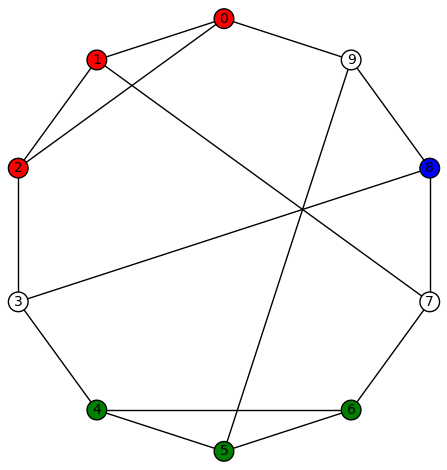
\includegraphics[height=5cm,width=5cm]{graphics/harmonic-quotient_d3reg10g-star4_3330111020.png}
\end{center}
\begin{center}
%\vspace{8.0 cm}
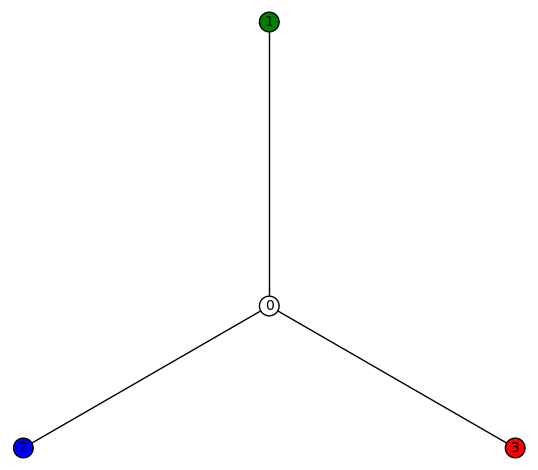
\includegraphics[height=5cm,width=4cm]{graphics/star4-0123.png}
\end{center}
\end{minipage}
\caption{The cubic graph  $\Gamma_2$ ({\tt d3reg10g}), a degree three harmonic quotient to the star graph, $St_4$.}
\label{fig:harmonic-quotient_d3reg10g-star4_3330111020}
\end{figure}

}
\end{example}


\begin{example}% d3reg10h
\label{example:d3reg10h}
  {\tt d3reg10h}\newline
{\rm  
Let $\Gamma_2$ have vertices

\[
V_2=\{0,1,\dots,9\}
\]
and edges

\[
E_2 = \{
(0, 1), (0, 5), (0, 9), (1, 2), (1, 4), (2, 3), (2, 7), (3, 4), 
\]
\[
(3, 9), (4, 5), (5, 6), (6, 7), (6, 8), (7, 8), (8, 9)
\}.
\]
This graph has no non-constant harmonic quotient
morphisms $\pi: \Gamma_2\to \Gamma_2/G$, for some subgroup
$G$ of $\Aut(\Gamma_2)$.

}
\end{example}


\begin{example}% d3reg10i
\label{example:d3reg10i}
  {\tt d3reg10i}\newline
{\rm  
Let $\Gamma_2$ have vertices

\[
V_2=\{0,1,\dots,9\}
\]
and edges

\[
E_2 = \{
(0, 1), (0, 6), (0, 9), (1, 2), (1, 4), (2, 3), (2, 5), (3, 4),
\]
\[
(3, 8), (4, 5), (5, 6), (6, 7), (7, 8), (7, 9), (8, 9)
\}.
\]
This graph has no non-constant harmonic quotient
morphisms $\pi: \Gamma_2\to \Gamma_2/G$, for some subgroup
$G$ of $\Aut(\Gamma_2)$.

}
\end{example}



\begin{example}% d3reg10j
\label{example:d3reg10j}
  {\tt d3reg10j}\newline
{\rm  
Let $\Gamma_2$ have vertices

\[
V_2=\{0,1,\dots,9\}
\]
and edges

\[
E_2 = \{
(0, 1), (0, 3), (0, 9), (1, 2), (1, 8), (2, 3), (2, 7), (3, 4),
\]
\[
(4, 5), (4, 6), (5, 6), (5, 9), (6, 7), (7, 8), (8, 9)
\}.
\]
This graph has no non-constant harmonic quotient
morphisms $\pi: \Gamma_2\to \Gamma_2/G$, for some subgroup
$G$ of $\Aut(\Gamma_2)$.

}
\end{example}


\begin{example}% d3reg10k
\label{example:d3reg10k}
  {\tt d3reg10k}\newline
{\rm  
Let $\Gamma_2$ have vertices

\[
V_2=\{0,1,\dots,9\}
\]
and edges

\[
E_2 = \{
(0, 1), (0, 6), (0, 9), (1, 2), (1, 5), (2, 3), (2, 4), (3, 4),
\]
\[
(3, 8), (4, 5), (5, 6), (6, 7), (7, 8), (7, 9), (8, 9)
\}.
\]
This graph has only $2$ non-constant harmonic quotient
morphisms $\pi: \Gamma_2\to \Gamma_2/G$, for some subgroup
$G$ of $\Aut(\Gamma_2)$. In this case,
$G = \langle (0,1)(2,9)(3,8)(4,7)(5,6) \rangle$ and
$\Gamma_1 =  \Gamma_2/G$ is the house graph, with vertices and edges:

\[
V_1 = \{0, \dots, 4\},
\]
\[
E_1 = \{(0, 3), (0, 4), (1, 2), (1, 4), (2, 3), (3, 4)\}.
\]
Note that vertices $3$ and $4$ are those with degree $3$.
(The other harmonic quotient is for $G=\Aut(\Gamma_2)$, of order $4$. It is a
quotient to $P_3$, with fibers $\{0,1,5,6\}$, $\{2,4,7,9\}$, $\{3,8\}$.)

The quotient morphism 
associated to this subgroup
is tabulated below. As we can see, it's a quasicover
$\phi:\Gamma_2\to \Gamma_1$.

\begin{center}
\begin{tabular}{c|c|c|c}  
  $x$ & $\phi(x)$ & $m_\phi(x)$ & $\nu_\phi(x)$ \\ \hline
  0   &    2   &        1         &  1   \\ 
  1   &    2   &        1         &  1   \\ 
  2   &    3   &        1         &  0   \\ 
  3   &    0   &        1         &  1   \\ 
  4   &    4   &        1         &  0   \\ 
  5   &    1   &        1         &  1    \\ 
  6   &    1   &        1         &  1   \\ 
  7   &    4   &        1         &  0   \\
  8   &    0   &        1         &  1   \\
  9   &    3   &        1         &  0   \\ 
\end{tabular}
\end{center}

\[
  \genus(\Gamma_2) =6,\ \ \ \ \
  \genus(\Gamma_1) =2,
\]

\[
\deg(\phi) =2.
\]
The uncolored graphs are depicted in Figure \ref{fig:harmonic-quotient_d3reg10k+house}.

\begin{figure}[H]
\begin{minipage}{\textwidth}
\begin{center}
%\vspace{8.0 cm}
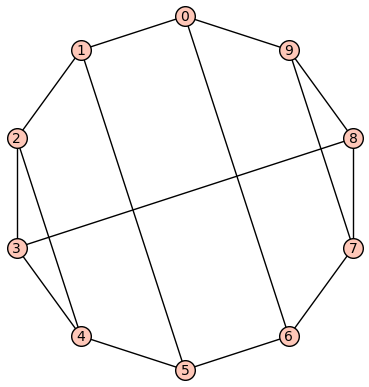
\includegraphics[height=5cm,width=5cm]{graphics/graph_d3reg10k.png}
\end{center}
\begin{center}
%\vspace{8.0 cm}
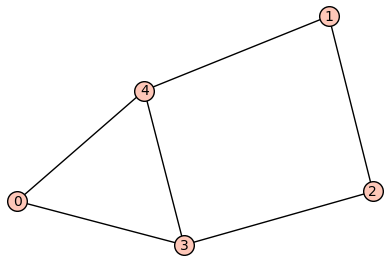
\includegraphics[height=5cm,width=4cm]{graphics/house-graph.png}
\end{center}
\end{minipage}
\caption{The cubic graph  $\Gamma_2$ ({\tt d3reg10k}), with a degree two harmonic quotient morphism to and quasicover of, the house graph, $\Gamma_1$.}
\label{fig:harmonic-quotient_d3reg10k+house}
\end{figure}

}
\end{example}



\begin{example}% d3reg10l
\label{example:d3reg10l}
  {\tt d3reg10l}\newline
{\rm  
Let $\Gamma_2$ have vertices

\[
V_2=\{0,1,\dots,9\}
\]
and edges

\[
E_2 = \{
(0, 1), (0, 5), (0, 9), (1, 2), (1, 9), (2, 3), (2, 4), (3, 4),
\]
\[
(3, 7), (4, 5), (5, 6), (6, 7), (6, 8), (7, 8), (8, 9)
\}.
\]
This graph has no non-constant harmonic quotient
morphisms $\pi: \Gamma_2\to \Gamma_2/G$, for some subgroup
$G$ of $\Aut(\Gamma_2)$.

}
\end{example}



\begin{example}% d3reg10m
\label{example:d3reg10m}
  {\tt d3reg10m}\newline
{\rm  
Let $\Gamma_2$ have vertices

\[
V_2=\{0,1,\dots,9\}
\]
and edges

\[
E_2 = \{
(0, 1), (0, 2), (0, 9), (1, 2), (1, 6), (2, 3), (3, 4), (3, 8), 
\]
\[
(4, 5), (4, 9), (5, 6), (5, 7), (6, 7), (7, 8), (8, 9)
\}.
\]
This graph has only $5$ non-constant harmonic quotient
morphisms $\pi: \Gamma_2\to \Gamma_2/G$, for some subgroup
$G$ of $\Aut(\Gamma_2)$.
For $2$ subgroups, the quotient $ \Gamma_2/G$ is isomorphic to the house graph
and the quotient morphisms are distinct. For the remaining three subgroups (one of which is $\Aut(\Gamma_2)$),
the quotient $ \Gamma_2/G$ is
isomorphic\footnote{The vertices are $0,1,2$, but their ordering is different that usual:
  $0$ and $1$ are the vertices of degree $1$, while vertex $2$ has degree $2$.}
  to $P_3$ and all three quotient morphisms are the same.

In case $G = \langle (0,5)(1,6)(2,7)(3,8)(4,9) \rangle$,
$\Gamma_1 =  \Gamma_2/G$ is the house graph, with vertices and edges:

\[
V_1 = \{0, \dots, 4\},
\]
\[
E_1 = \{(0, 1), (0, 2), (1, 4), (2, 3), (2, 4), (3, 4)\}.
\]
Note that vertices $2$ and $4$ are those with degree $3$.
The quotient morphism 
associated to this subgroup $G$ is tabulated below. As we can see, it's a quasicover
$\phi:\Gamma_2\to \Gamma_1$.

\begin{center}
\begin{tabular}{c|c|c|c}  
  $x$ & $\phi(x)$ & $m_\phi(x)$ & $\nu_\phi(x)$ \\ \hline
  0   &    4   &        1         &  0   \\ 
  1   &    3   &        1         &  1   \\ 
  2   &    2   &        1         &  0   \\ 
  3   &    0   &        1         &  1   \\ 
  4   &    1   &        1         &  1   \\ 
  5   &    4   &        1         &  0    \\ 
  6   &    3   &        1         &  1   \\ 
  7   &    2   &        1         &  0   \\
  8   &    0   &        1         &  1   \\
  9   &    1   &        1         &  1   \\ 
\end{tabular}
\end{center}

\[
  \genus(\Gamma_2) =6,\ \ \ \ \
  \genus(\Gamma_1) =2,
\]

\[
\deg(\phi) =2.
\]

The quotient morphism $\phi:\Gamma_2\to \Gamma_1=P_3$
associated to the subgroup
\[
G = \langle (0,2)(3,9)(4,8)(5,7), (0,5)(1,6)(2,7)(3,8)(4,9) \rangle
\]
is tabulated below.

\begin{center}
\begin{tabular}{c|c|c|c}  
  $x$ & $\phi(x)$ & $m_\phi(x)$ & $\nu_\phi(x)$ \\ \hline
  0   &    2   &        1         &  1   \\ 
  1   &    0   &        2         &  1   \\ 
  2   &    2   &        1         &  1   \\ 
  3   &    1   &        1         &  2   \\ 
  4   &    1   &        1         &  2   \\ 
  5   &    2   &        1         &  1    \\ 
  6   &    0   &        2         &  1   \\ 
  7   &    2   &        1         &  1   \\
  8   &    1   &        1         &  2   \\
  9   &    1   &        1         &  2   \\ 
\end{tabular}
\end{center}

\[
  \genus(\Gamma_2) =6,\ \ \ \ \
  \genus(\Gamma_1) =0,
\]

\[
\deg(\phi) =4.
\]

}
\end{example}




\begin{example}% d3reg10n
\label{example:d3reg10n}
  {\tt d3reg10n}\newline
{\rm  
Let $\Gamma_2$ have vertices

\[
V_2=\{0,1,\dots,9\}
\]
and edges

\[
E_2 = \{
(0, 1), (0, 5), (0, 9), (1, 2), (1, 8), (2, 3), (2, 9), (3, 4),
\]
\[
(3, 6), (4, 5), (4, 7), (5, 6), (6, 7), (7, 8), (8, 9)
\}.
\]
This graph has $32$ non-constant harmonic quotient
morphisms $\pi: \Gamma_2\to \Gamma_2/G$, for some subgroup
$G$ of $\Aut(\Gamma_2)$.

Two of these groups yield the same harmonic quotient morphism to
the ``$H$-tree'' - a genus $0$ graph $\Gamma_1 = (V_1,E_1)$
with vertices and edges,

\[
V_1=\{0,1,\dots, 5\},
\]
\[
E_1=\{
(0, 1), (0, 3), (0, 5), (1, 2), (1, 4)
\}.
\]
For example, the group $G=\langle (0,8,2)(3,5,7) \rangle$
yields this quotient graph $\Gamma_1=\Gamma_2/G$.

Two of these groups yield (two distinct) harmonic quotient morphisms to
$K_{2,3}$ - a genus $2$ graph $\Gamma_1 = (V_1,E_1)$
with vertices and edges,

\[
V_1=\{0,1,\dots, 4\},
\]
\[
E_1=\{
(0, 2), (0, 3), (0, 4), (1, 2), (1, 3), (1, 4)
\}.
\]
For example, the group $G=\langle (0,5)(1,4)(2,3)(6,9)(7,8) \rangle$
yields this quotient graph $\Gamma_1=\Gamma_2/G$.
One of these is tabulated below and the uncolored graphs are
depicted in Figure \ref{fig:harmonic-quotient_d3reg10n+K23}.
\begin{center}
\begin{tabular}{c|c|c|c}  
  $x$ & $\phi(x)$ & $m_\phi(x)$ & $\nu_\phi(x)$ \\ \hline
  0   &    3   &        1         &  1   \\ 
  1   &    1   &        1         &  0   \\ 
  2   &    2   &        1         &  1   \\ 
  3   &    2   &        1         &  1   \\ 
  4   &    1   &        1         &  0   \\ 
  5   &    3   &        1         &  1    \\ 
  6   &    0   &        1         &  0   \\ 
  7   &    4   &        1         &  1   \\
  8   &    4   &        1         &  1   \\
  9   &    0   &        1         &  0   \\ 
\end{tabular}
\end{center}

\[
  \genus(\Gamma_2) =6,\ \ \ \ \
  \genus(\Gamma_1) =2,
\]

\[
\deg(\phi) =2.
\]

\begin{figure}[H]
\begin{minipage}{\textwidth}
\begin{center}
%\vspace{8.0 cm}
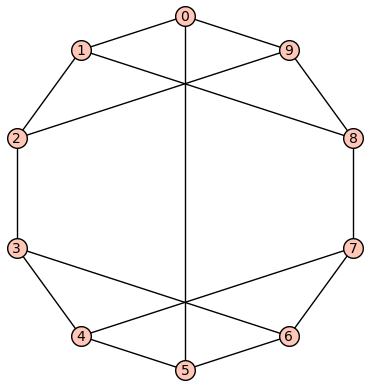
\includegraphics[height=5cm,width=5cm]{graphics/graph_d3reg10n.png}
\end{center}
\begin{center}
%\vspace{8.0 cm}
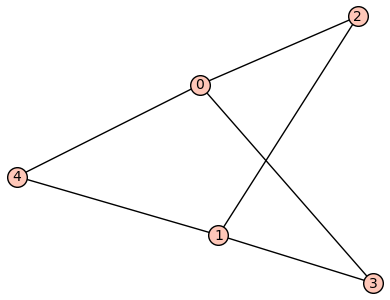
\includegraphics[height=5cm,width=4cm]{graphics/complete-bipartite-K-2-3.png}
\end{center}
\end{minipage}
\caption{The cubic graph  $\Gamma_2$ ({\tt d3reg10n}), with a degree two harmonic quotient morphism to and quasicover of, the complete bipartite graph, $\Gamma_1=K_{2,3}$.}
\label{fig:harmonic-quotient_d3reg10n+K23}
\end{figure}

Three of these groups yield the same harmonic quotient morphism to
$St_4$, the star graph on $4$ vertices.
\index{star graph}

Six further groups (each of order $2$) yield six distinct degree two
harmonic quotient morphisms to the genus $3$ graph $\overline{P_2\cup P_3}$
($5$ vertices, $7$ edges).

The remaining $19$ harmonic quotient morphisms are to $P_3$ ($6$ groups,
$2$ distinct morphisms) or to $P_2$ ($13$ groups, one of them $\Aut(\Gamma_2)$,
all give the same morphism).

}
\end{example}





\begin{example}% d3reg10o
\label{example:d3reg10o}
  {\tt d3reg10o}\newline
{\rm  
Let $\Gamma_2$ have vertices

\[
V_2=\{0,1,\dots,9\}
\]
and edges

\[
E_2 = \{
(0, 1), (0, 5), (0, 9), (1, 2), (1, 7), (2, 3), (2, 6), (3, 4),
\]
\[
(3, 9), (4, 5), (4, 8), (5, 6), (6, 7), (7, 8), (8, 9)
\}.
\]
This graph has $3$ non-constant harmonic quotient
morphisms $\pi: \Gamma_2\to \Gamma_2/G$, for some subgroup
$G$ of $\Aut(\Gamma_2)$.

The group $G = \langle (0,5)(1,4)(2,3)(6,9)(7,8) \rangle$ yields the
harmonic quotient morphism to the genus $2$ graph
$\Gamma_1 = (V_1,E_1) = K_{2,3}$
with vertices and edges,

\[
V_1=\{0,1,\dots, 4\},
\]
\[
E_1=\{
(0, 2), (0, 3), (0, 4), (1, 2), (1, 3), (1, 4)
\}.
\]
This is tabulated below (and agrees with a table in a previous example).

\begin{center}
\begin{tabular}{c|c|c|c}  
  $x$ & $\phi(x)$ & $m_\phi(x)$ & $\nu_\phi(x)$ \\ \hline
  0   &    3   &        1         &  1   \\ 
  1   &    1   &        1         &  0   \\ 
  2   &    2   &        1         &  1   \\ 
  3   &    2   &        1         &  1   \\ 
  4   &    1   &        1         &  0   \\ 
  5   &    3   &        1         &  1    \\ 
  6   &    0   &        1         &  0   \\ 
  7   &    4   &        1         &  1   \\
  8   &    4   &        1         &  1   \\
  9   &    0   &        1         &  0   \\ 
\end{tabular}
\end{center}

\[
  \genus(\Gamma_2) =6,\ \ \ \ \
  \genus(\Gamma_1) =2,
\]

\[
\deg(\phi) =2.
\]

The group $G = \langle (0,5)(1,4)(2,8)(3,7)(6,9) \rangle$ yields the
harmonic quotient morphism to the genus $3$ graph
$\Gamma_1 = (V_1,E_1)$
with vertices and edges,

\[
V_1=\{0,1,\dots, 4\},
\]
\[
E_1=\{
(0, 1), (0, 2), (0, 3), (1, 3), (1, 4), (2, 3), (2, 4)
\}.
\]
This is tabulated below.

\begin{center}
\begin{tabular}{c|c|c|c}  
  $x$ & $\phi(x)$ & $m_\phi(x)$ & $\nu_\phi(x)$ \\ \hline
  0   &    4   &        1         &  1   \\
  1   &    2   &        1         &  0   \\
  2   &    0   &        1         &  0   \\
  3   &    3   &        1         &  0   \\
  4   &    2   &        1         &  0   \\
  5   &    4   &        1         &  1   \\
  6   &    1   &        1         &  0   \\
  7   &    3   &        1         &  0   \\
  8   &    0   &        1         &  0   \\
  9   &    1   &        1         &  0   \\
\end{tabular}
\end{center}

\[
  \genus(\Gamma_2) =6,\ \ \ \ \
  \genus(\Gamma_1) =3,
\]

\[
\deg(\phi) =2.
\]

Finally, the group
$G = \langle (1,9)(2,3)(4,6)(7,8), (0,5)(1,6)(4,9) \rangle$ yields the
harmonic quotient morphism to the genus $0$ graph
$\Gamma_1 = (V_1,E_1) = St_4$, with

\[
V_1=\{0, 1, 2, 3\},
\]
and $0$ is the degree $3$ (``center'') vertex.
This is tabulated below.

\begin{center}
\begin{tabular}{c|c|c|c}  
  $x$ & $\phi(x)$ & $m_\phi(x)$ & $\nu_\phi(x)$ \\ \hline
  0   &    3   &        2         &  1   \\ 
  1   &    0   &        1         &  0   \\ 
  2   &    1   &        2         &  1   \\ 
  3   &    1   &        2         &  1   \\ 
  4   &    0   &        1         &  0   \\ 
  5   &    3   &        2         &  1    \\ 
  6   &    0   &        1         &  0   \\ 
  7   &    2   &        2         &  1   \\
  8   &    2   &        2         &  1   \\
  9   &    0   &        1         &  0   \\ 
\end{tabular}
\end{center}

\[
  \genus(\Gamma_2) =6,\ \ \ \ \
  \genus(\Gamma_1) =0,
\]

\[
\deg(\phi) =4.
\]


}
\end{example}



\begin{example}% d3reg10p
\label{example:d3reg10p}
  {\tt d3reg10p}\newline
{\rm  
Let $\Gamma_2$ have vertices

\[
V_2=\{0,1,\dots,9\}
\]
and edges

\[
E_2 = \{
(0, 1), (0, 5), (0, 9), (1, 2), (1, 7), (2, 3), (2, 6), (3, 4), 
\]
\[
 (3, 8), (4, 5), (4, 9), (5, 6), (6, 7), (7, 8), (8, 9)
\}.
\]
This graph has only $2$ non-constant harmonic quotient
morphisms $\pi: \Gamma_2\to \Gamma_2/G$, for some subgroup
$G$ of $\Aut(\Gamma_2)$.


The group $G = \langle (0,3)(1,2)(4,9)(5,8)(6,7) \rangle$ yields the
harmonic quotient morphism to the house graph
$\Gamma_1 = (V_1,E_1)$
with vertices and edges,

\[
V_1=\{0,1,\dots, 4\},
\]
\[
E_1=\{
(0, 1), (0, 3), (1, 2), (1, 4), (2, 4), (3, 4)
\}.
\]
This is tabulated below. (The other harmonic quotient is for
$G=\Aut(\Gamma_2)$, of order $4$. It is a quotient to $P_3$, with fibers
$\{0,3,5,8\}$, $\{1,2,6,7\}$, $\{4,9\}$.)

\begin{center}
\begin{tabular}{c|c|c|c}  
  $x$ & $\phi(x)$ & $m_\phi(x)$ & $\nu_\phi(x)$ \\ \hline
  0   &    1   &        1         &  0   \\ 
  1   &    0   &        1         &  1   \\ 
  2   &    0   &        1         &  1   \\ 
  3   &    1   &        1         &  0   \\ 
  4   &    2   &        1         &  1   \\ 
  5   &    4   &        1         &  0    \\ 
  6   &    3   &        1         &  1   \\ 
  7   &    3   &        1         &  1   \\
  8   &    4   &        1         &  0   \\
  9   &    2   &        1         &  1   \\ 
\end{tabular}
\end{center}

\[
  \genus(\Gamma_2) =6,\ \ \ \ \
  \genus(\Gamma_1) =2,
\]

\[
\deg(\phi) =2.
\]

}
\end{example}





\begin{example}% d3reg10q
\label{example:d3reg10q}
  {\tt d3reg10q}\newline
{\rm  
Let $\Gamma_2$ have vertices

\[
V_2=\{0,1,\dots,9\}
\]
and edges

\[
E_2 = \{
(0, 1), (0, 5), (0, 9), (1, 2), (1, 6), (2, 3), (2, 9), (3, 4), 
\]
\[
(3, 8), (4, 5), (4, 7), (5, 6), (6, 7), (7, 8), (8, 9)
\}.
\]
This graph has $13$ non-constant harmonic quotient
morphisms $\pi: \Gamma_2\to \Gamma_2/G$, for some subgroup
$G$ of $\Aut(\Gamma_2)$.

Five of these quotient graphs are the house graph (each with a
distinct quotient morphism),
another five of these quotient graphs are the path graph $P_3$
(also with distinct quotient morphisms), 
however, the two groups that yield $P_2$ as a quotient have the
same quotient morphism.
Finally, the
 group $G = \langle (0,1)(2,9)(3,8)(4,7)(5,6) \rangle$ yields the
harmonic quotient morphism to the cycle graph
$\Gamma_1 = (V_1,E_1) = C_5$
with vertices and edges,

\[
V_1=\{0,1,\dots, 4\},
\]
\[
E_1=\{
(0, 3), (0, 4), (1, 2), (1, 4), (2, 3)
\}.
\]
This is tabulated below.

\begin{center}
\begin{tabular}{c|c|c|c}  
  $x$ & $\phi(x)$ & $m_\phi(x)$ & $\nu_\phi(x)$ \\ \hline
  0   &    2   &        1         &  1   \\ 
  1   &    2   &        1         &  1   \\ 
  2   &    3   &        1         &  1   \\ 
  3   &    0   &        1         &  1   \\ 
  4   &    4   &        1         &  1   \\ 
  5   &    1   &        1         &  1    \\ 
  6   &    1   &        1         &  1   \\ 
  7   &    4   &        1         &  1   \\
  8   &    0   &        1         &  1   \\
  9   &    3   &        1         &  1   \\ 
\end{tabular}
\end{center}

\[
  \genus(\Gamma_2) =6,\ \ \ \ \
  \genus(\Gamma_1) =1,
\]

\[
\deg(\phi) =2.
\]


\begin{figure}[H]
\begin{minipage}{\textwidth}
\begin{center}
%\vspace{8.0 cm}
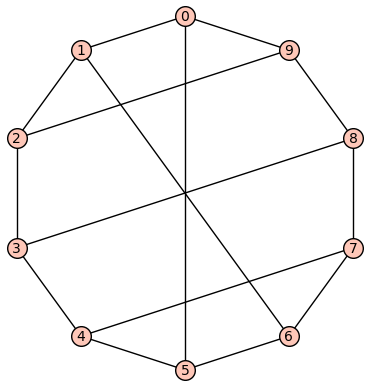
\includegraphics[height=5cm,width=5cm]{graphics/graph_d3reg10q.png}
\end{center}
\begin{center}
%\vspace{8.0 cm}
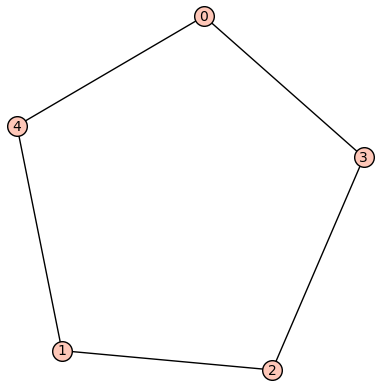
\includegraphics[height=5cm,width=4cm]{graphics/C5-quotient-of-d3reg10q.png}
\end{center}
\end{minipage}
\caption{The cubic graph  $\Gamma_2$ ({\tt d3reg10q}), with a degree two harmonic quotient morphism to and quasicover of, the cycle graph, $\Gamma_1=C_5$.}
\label{fig:harmonic-quotient_d3reg10q+C5}
\end{figure}

}
\end{example}




\begin{example}% d3reg10r
\label{example:d3reg10r}
  {\tt d3reg10r}\newline
{\rm  
Let $\Gamma_2$ have vertices

\[
V_2=\{0,1,\dots,9\}
\]
and edges

\[
E_2 = \{
(0, 1), (0, 6), (0, 9), (1, 2), (1, 5), (2, 3), (2, 9), (3, 4), 
\]
\[
(3, 8), (4, 5), (4, 7), (5, 6), (6, 7), (7, 8), (8, 9)
\}.
\]
This graph has $8$ non-constant harmonic quotient
morphisms $\pi: \Gamma_2\to \Gamma_2/G$, for some subgroup
$G$ of $\Aut(\Gamma_2)$.

Five of these quotient graphs are the path graph $P_3$
(with distinct quotient morphisms), 
however, the two groups that yield $P_2$ as a quotient have the
same quotient morphism.
Finally, the
group

\[
G = \langle (0,1)(2,9)(3,8)(4,7)(5,6) \rangle
\]
yields the
harmonic quotient morphism to the cycle graph
$\Gamma_1 = (V_1,E_1) = C_5$
with vertices and edges,

\[
V_1=\{0,1,\dots, 4\},
\]
\[
E_1=\{
(0, 3), (0, 4), (1, 2), (1, 4), (2, 3)
\}.
\]
This is tabulated below (the same table as in the previous example).

\begin{center}
\begin{tabular}{c|c|c|c}  
  $x$ & $\phi(x)$ & $m_\phi(x)$ & $\nu_\phi(x)$ \\ \hline
  0   &    2   &        1         &  1   \\ 
  1   &    2   &        1         &  1   \\ 
  2   &    3   &        1         &  1   \\ 
  3   &    0   &        1         &  1   \\ 
  4   &    4   &        1         &  1   \\ 
  5   &    1   &        1         &  1    \\ 
  6   &    1   &        1         &  1   \\ 
  7   &    4   &        1         &  1   \\
  8   &    0   &        1         &  1   \\
  9   &    3   &        1         &  1   \\ 
\end{tabular}
\end{center}

\[
  \genus(\Gamma_2) =6,\ \ \ \ \
  \genus(\Gamma_1) =1,
\]

\[
\deg(\phi) =2.
\]

}
\end{example}



\begin{example}% d3reg10s
\label{example:d3reg10s}
  {\tt d3reg10s}\newline
{\rm  
Let $\Gamma_2$ be the Petersen graph with vertices

\[
V_2=\{0,1,\dots,9\}
\]
and edges

\[
E_2 = \{
(0, 1), (0, 4), (0, 5), (1, 2), (1, 6), (2, 3), (2, 7), (3, 4),
\]
\[
(3, 8), (4, 9), (5, 7), (5, 8), (6, 8), (6, 9), (7, 9)
\}.
\]
This graph has $27$ non-constant harmonic quotient
morphisms $\pi: \Gamma_2\to \Gamma_2/G$, for some subgroup
$G$ of $\Aut(\Gamma_2)$. Five of these quotient graphs are 
the star graph with $4$ vertices, $St_4$, while the remaining
graphs are the path graph, $P_2$.
\index{star graph}

The group
$G = \langle (2,6)(3,8)(4,5)(7,9), (0,1)(2,4)(5,6)(7,9) \rangle$ yields the
harmonic quotient morphism to the genus $0$ graph
$\Gamma_1 = (V_1,E_1) = St_4$, with

\[
V_1=\{0, 1, 2, 3\},
\]
and $3$ is the degree $3$ (``center'') vertex.
This is tabulated below.

\begin{center}
\begin{tabular}{c|c|c|c}  
  $x$ & $\phi(x)$ & $m_\phi(x)$ & $\nu_\phi(x)$ \\ \hline
  0   &    1   &        2         &  1   \\ 
  1   &    1   &        2         &  1   \\ 
  2   &    3   &        1         &  0   \\ 
  3   &    0   &        2         &  1   \\ 
  4   &    3   &        1         &  0   \\ 
  5   &    3   &        1         &  0    \\ 
  6   &    3   &        1         &  0   \\ 
  7   &    2   &        2         &  1   \\
  8   &    0   &        2         &  1   \\
  9   &    2   &        2         &  1   \\ 
\end{tabular}
\end{center}

\[
  \genus(\Gamma_2) =6,\ \ \ \ \
  \genus(\Gamma_1) =0,
\]

\[
\deg(\phi) =4.
\]

}
\end{example}




\subsection{\texorpdfstring{$12$}{12} vertices}
\label{sec:cubic-12-vertices}

This subsection describes a selection of the connected cubic graphs on $12$ vertices.
It records their invariants and harmonic morphism counts, and then
works out harmonic quotient morphisms in examples.

%%% file-of-d3reg12-graphs.txt and  file-of-3reg12-graphs.txt

There are $85$ non-isomorphic, connected, cubic graphs on $12$ vertices,
$80$ of which are Hamiltonian and $4$ of which are vertex transitive.
However, none of the $85$ graphs
in this collection are edge transitive.

Here are several examples,
including those $4$ which are vertex transitive and
four of the five that are not Hamiltonian.


{\small{
\begin{center}
\begin{tabular}{c|c|c|c}
  graph label & LCF & $|\Aut(\Gamma)|$ & genus  \\ \hline
  d3reg12a & -- & 16 & 7   \\
  d3reg12b & -- & 16 & 7  \\
  d3reg12c & -- & 8 & 7   \\
  d3reg12d & -- & 32 & 7  \\
  d3reg12e & (12, [3, -2, -4, -3, 4, 2], 2) & 4 & 7  \\
  d3reg12f & (12, [3,-2,-4,-3,3,3,3,-3,-3,-3,4,2], 1) & 8 & 7   \\
  d3reg12g & (12, [4,2,3,-2,-4,-3,2,3,-2,2,-3,-2], 1) & 4 & 7  \\
  d3reg12h & (12, [3, 3, 3, -3, -3, -3], 2) & 64 & 7  \\
  d3reg12i & (12, [2,-3,-2,3,3,3,-3,-3,-3,2,3,-2], 1) & 16 & 7   \\
  d3reg12j & (12, [2, 3, -2, 2, -3, -2], 2) & 16 & 7  \\
  d3reg12k & (12, [-2,3,6,3,-3,2,-3,-2,6,2,2,-2], 1) & 2 & 7  \\
  d3reg12l & (12, [6, -2, 2], 4) & 24 & 7  \\
  d3reg12m & (12, [-3, 3], 6) & 24 & 7  \\
  d3reg12n & (12, [5, -5], 6) & 48 & 7  \\
  
\end{tabular}
\end{center}  
}}



\begin{enumerate}
\item
  {\tt d3reg12a}\newline % or #83
  The one with vertices and edges:

\[
V=\{ 0,1,2,3,4,5,6,7,8,9,10,11\},
\]
\[
E = \{
(0, 1), (0, 2), (0, 9), (1, 2), (1, 3), (2, 3), (3, 9), (4, 5), (4, 6), (4, 7),
\]
\[
 (5, 8), (5, 11), (6, 7), (6, 10), (7, 10), (8, 9), (8, 11), (10, 11)
\},
\]
has automorphism group of order $16$ and
characteristic polynomial  
\[
x^{12} - 18x^{10} - 10x^9 + 109x^8 + 112x^7 - 223x^6 - 326x^5 + 58x^4 + 196x^3 + 9x^2 - 36x.
\]
It has girth $3$ and diameter $6$.
This is {\it not} a Hamiltonian graph, with circumference $7$.
The cardinality of its critical group is $2112=2^63\cdot 11$.

It has no non-trivial harmonic morphisms to $St_4$ or $P_4$, $C_3$, $C_4$,
or to $K_4$.
However, there are $8$ non-trivial harmonic morphisms to $P_3$.

%At this time, the number of non-trivial harmonic morphisms to $K_4$ is unknown.


\item
  {\tt d3reg12b}\newline % or #60
The one with vertices and edges:

\[
V=\{ 0,1,2,3,4,5,6,7,8,9,10,11\},
\]
\[
E = \{
(0, 1), (0, 9), (0, 10), (1, 4), (1, 5), (2, 3), (2, 6), (2, 11), (3, 6), 
\]
\[
(3, 9), (4, 5), (4, 10), (5, 10), (6, 7), (7, 8), (7, 11), (8, 9), (8, 11)
\}
\]
has automorphism group of order $16$ and
characteristic polynomial  
\[
x^{12} - 18x^{10} - 8x^9 + 109x^8 + 84x^7 - 240x^6 - 220x^5 + 172x^4 + 168x^3 .
\]
It has girth $3$ and diameter $5$.
This is {\it not} a Hamiltonian graph, with circumference $7$.
The size of the critical group of this graph is $2520=2^33^25\cdot 7$.

It has no non-trivial harmonic morphisms to $St_4$, $P_4$, $C_4$, or to $K_4$.
However, it has $14$ non-trivial harmonic morphisms to $P_3$ and
$6$ non-trivial harmonic morphisms to $C_3$.

\item
  {\tt d3reg12c}\newline % or #41
  The one with vertices and edges:

\[
V=\{ 0,1,2,3,4,5,6,7,8,9,10,11\},
\]
\[
E = \{
(0, 1), (0, 10), (0, 11), (1, 3), (1, 4), (2, 3), (2, 5), (2, 11), (3, 5),
\]
\[
(4, 5), (4, 11), (6, 7), (6, 8), (6, 10), (7, 8), (7, 9), (8, 9), (9, 10)
\}.
\]
has automorphism group of order $8$ and
characteristic polynomial  
\[
x^{12} - 18x^{10} - 6x^9 + 105x^8 + 60x^7 - 211x^6 - 122x^5 + 146x^4 + 52x^3 - 39x^2 .
\]
It has girth $3$ and diameter $6$.
This is {\it not} a Hamiltonian graph, with circumference $7$.
The size of the critical group of this graph is $2640=2^43\cdot 5\cdot 11$.

It has no non-trivial harmonic morphisms to $St_4$, $P_4$, $C_3$, $C_4$, or to $K_4$.
However, it has $6$ non-trivial harmonic morphisms to $P_3$.


\item
  {\tt d3reg12d}\newline % or 40
The one with vertices and edges:

\[
V=\{ 0,1,2,3,4,5,6,7,8,9,10,11\},
\]
\[
E = \{
(0, 1), (0, 10), (0, 11), (1, 3), (1, 4), (2, 3), (2, 4), (2, 11), (3, 5),
\]
\[
(4, 5), (5, 11), (6, 7), (6, 8), (6, 10), (7, 8), (7, 9), (8, 9), (9, 10)
\}.
\]
has automorphism group of order $32$ and
characteristic polynomial  
\[
x^{12} - 18x^{10} - 4x^9 + 101x^8 + 36x^7 - 176x^6 - 40x^5 + 84x^4 .
\]
It has girth $3$ and diameter $5$.
This is {\it not} a Hamiltonian graph, with circumference $7$.
The size of the critical group of this graph is $2808=2^33^313$.

It has $12$ non-trivial harmonic morphisms to $St_4$,
$22$ non-trivial harmonic morphisms to $P_3$, 
$12$ non-trivial harmonic morphisms to $C_3$, but
no non-trivial harmonic morphisms to $P_4$, $C_4$, or to $K_4$.


\item
  {\tt d3reg12e}\newline % or #33
 The one with automorphism group of order $4$ and
characteristic polynomial  
\[
x^{12} - 18x^{10} - 4x^9 + 109x^8 + 36x^7 - 256x^6 - 64x^5 + 228x^4 + 16x^3 - 48x^2 
\]
has girth $3$ and diameter $5$.
This is a Hamiltonian graph (with circumference $12$).
The size of the critical group of this graph is $5250=2\cdot 3\cdot 5^37$.

It has no non-trivial harmonic morphisms to $St_4$, $P_4$, $C_4$, or to $K_4$.
However, it has $4$ non-trivial harmonic morphisms to $P_3$ and
$6$ non-trivial harmonic morphisms to $C_3$.

SageMath notation:

\verb@graphs.LCFGraph(12,[3, -2, -4, -3, 4, 2], 2)@


\item
  {\tt d3reg12f}\newline % or #32
The one with automorphism group of order $8$ and
having characteristic polynomial  
\[
x^{12} - 18x^{10} - 2x^9 + 103x^8 + 18x^7 - 201x^6 - 26x^5 + 105x^4 
\]
has girth $3$ and diameter $4$.
This is a Hamiltonian graph (with circumference $12$).
The size of the critical group of this graph is $5535=3^35\cdot 41$.

It has $12$ non-trivial harmonic morphisms to $P_3$,
$36$ non-trivial harmonic morphisms to $C_3$, and
$12$ non-trivial harmonic morphisms to $St_4$.
However, there were no
non-trivial harmonic morphisms to $P_4$, $C_4$, or to $K_4$.

SageMath notation:

\verb@graphs.LCFGraph(12,[3,-2,-4,-3,3,3,3,-3,-3,-3,4,2],1)@



\item
  {\tt d3reg12g}\newline % or #31
The one with automorphism group of order $4$ and
having characteristic polynomial  
\[
x^{12} - 18x^{10} - 6x^9 + 111x^8 + 62x^7 - 265x^6 - 166x^5 + 213x^4 + 92x^3 - 60x^2 
\]
has girth $3$ and diameter $4$.
This is a Hamiltonian graph (with circumference $12$).
The size of the critical group of this graph is $4875=3\cdot 5^313$.

It has $6$ non-trivial harmonic morphisms to $C_3$, but no
non-trivial harmonic morphisms to $St_4$, $P_3$, $P_4$, $C_4$, or to $K_4$.

SageMath notation:

\verb@graphs.LCFGraph(12,[4,2,3,-2,-4,-3,2,3,-2,2,-3,-2],1)@


\item
  {\tt d3reg12h}\newline % or #4
The one with automorphism group of order $64$ and
characteristic polynomial  
\[
x^{12} - 18x^{10} + 97x^8  - 144x^6 
\]
has girth $4$ and diameter $4$.
This is a bipartite, Hamiltonian graph (with circumference $12$).
The size of the critical group of this graph is $5832=2^33^6$.

It
has\footnote{Not only is $168$ some sort of record for
  the data we are looking at here, some of these are quasicovers
  (where the horizontal multiplicity, as a function of the
  vertices of $\Gamma$, is the constant $1$). One of these has a weed
  with $6$ roots (see Remark~\ref{rem:weed}).}
$168$ non-trivial harmonic morphisms to $C_3$,
$48$ non-trivial harmonic morphisms to $St_4$,
$56$ non-trivial harmonic morphisms to $P_3$, but no
non-trivial harmonic morphisms to $P_4$, $C_4$, or to $K_4$.

SageMath notation:

\verb@graphs.LCFGraph(12, [3, 3, 3, -3, -3, -3], 2)@


\item
  {\tt d3reg12i}\newline % or #3
The one with automorphism group of order $16$ and
having characteristic polynomial  

\[
x^{12} - 18x^{10} - 4x^9 + 105x^8 + 44x^7 - 216x^6 - 104x^5 + 96x^4 
\]
has girth $3$ and diameter $4$.
This is a Hamiltonian graph (with circumference $12$).
The size of the critical group of this graph is $5130=2\cdot 3^35\cdot 19$.

It has $42$ non-trivial harmonic morphisms to $C_3$,
$12$ non-trivial harmonic morphisms to $P_3$,
$12$ non-trivial harmonic morphisms to $St_4$,
but no
non-trivial harmonic morphisms to $P_4$, $C_4$, or to $K_4$.

SageMath notation:

\verb@graphs.LCFGraph(12,[2,-3,-2,3,3,3,-3,-3,-3,2,3,-2],1)@


\item
  {\tt d3reg12j}\newline % or #28
The one with automorphism group of order $16$ and
having characteristic polynomial  
\[
x^{12} - 18x^{10} - 8x^9 + 113x^8 + 88x^7 - 272x^6 - 272x^5 + 176x^4 + 192x^3
\]
has girth $3$ and diameter $4$.
This is a Hamiltonian graph (with circumference $12$).
The size of the critical group of this graph is $4500=2^23^25^3$.

It has $24$ non-trivial harmonic morphisms to $P_3$,
$24$ non-trivial harmonic morphisms to $C_3$,
$2$ non-trivial harmonic morphisms to $P_4$, but no
non-trivial harmonic morphisms to $St_4$, $C_4$, or to $K_4$.
By a computer check using SageMath we know there
are no non-trivial harmonic morphisms to $P_5$.
%Using Theorem \ref{thrm:diameter-bound}
Therefore, we know there
are no non-trivial harmonic morphisms to $P_k$, for $k\geq 5$.

SageMath notation:

\verb@graphs.LCFGraph(12, [2, 3, -2, 2, -3, -2], 2)@


\item
  {\tt d3reg12k}\newline % or #66
The one with automorphism group of order $2$ and
having characteristic polynomial  

\[
x^{12} - 18x^{10} - 6x^9 + 111x^8 + 68x^7 - 275x^6 - 220x^5 + 257x^4 + 236x^3 - 61x^2 - 54x + 9
\]
has girth $3$ and diameter $4$.
This is a Hamiltonian graph (with circumference $12$).
The size of the critical group of this graph is $5104=2^411\cdot 29$.

It has no non-trivial harmonic morphisms to $St_4$, $C_3$, $C_4$, $P_4$, or to $K_4$.
However, it has $4$ non-trivial harmonic morphisms to $P_3$.

%At this time, the number of non-trivial harmonic morphisms to $K_4$ is unknown.

SageMath notation:

\verb@graphs.LCFGraph(12,[-2,3,6,3,-3,2,-3,-2,6,2,2,-2],1)@


\item
  {\tt d3reg12l}\newline %{\tt d3reg12-17}
The truncated tetrahedron graph with automorphism group of order $24$
(a group isomorphic to $S_4$ acting transitively on the vertices)
has characteristic polynomial  
\index{truncated tetrahedron graph}
  
\[
x^{12} - 18x^{10} - 8x^9 + 117x^8 + 96x^7 - 316x^6 - 384x^5 + 240x^4 + 512x^3 + 192x^2 \, .
\]
This graph has chromatic number $3$ and is not edge transitive.
It has girth $3$, diameter $3$, and
is a Hamiltonian graph (with circumference $12$).
The size of the critical group of this graph is $6000=2^43\cdot 5^3$.

This graph has $12$ non-trivial harmonic morphisms to $P_3$,
$6$ non-trivial harmonic morphisms to $C_3$,
$6$ non-trivial harmonic morphisms to $P_4$,
$24$ non-trivial harmonic morphisms\footnote{All 24 of
  these non-trivial harmonic morphisms of $\Gamma_2\to\Gamma_1=K_4$
  are covers of degree $3$
  and are permuted amongst each other by the automorphism group.}
to $K_4$, but
no non-trivial harmonic morphisms to $C_4$ or to $St_4$.
All the non-trivial harmonic morphisms to $K_4$ are covers
and they are permuted transitively under the action of the
automorphism group of the graph.

SageMath notation:

\verb@graphs.LCFGraph(12, [6, -2, 2], 4)@


\item
  {\tt d3reg12m}\newline %{\tt d3reg12-11}
The graph, $\Gamma$ say, with automorphism group of order $24$
(acting transitively on the vertices) has characteristic polynomial  

\[
x^{12} - 18x^{10} + 105x^8 - 232x^6 + 144x^4  \, .
\]
It is an integral graph\footnote{Its adjacency spectrum
multi-set  is $\{3, 2, 2, 1, 0, 0, 0, 0, -1, -2, -2, -3\}$.},
with girth $4$, diameter $4$, and
circumference $12$ (i.e., is a Hamiltonian graph). 
It is bipartite but not edge transitive.
The size of the critical group of this graph
is\footnote{Note there is another
cubic graph, $\Gamma'$ say, on $12$ vertices, not presented here,
having this size critical group but trivial automorphism group:
$|\Aut(\Gamma')|=1$. In particular, $\Gamma'$ is not a transitive graph.}
$8100=2^23^45^2$.
\index{integral graph}

There are no non-trivial harmonic morphisms to $C_4$ or to $K_4$.
However, there are $30$ non-trivial harmonic morphisms to $P_3$
$6$ non-trivial harmonic morphisms to $P_4$,
$12$ non-trivial harmonic morphisms to $St_4$, and
$36$ non-trivial harmonic morphisms\footnote{All these
  morphisms are quasicovers, with constant horizontal multiplicity
  $1$ and constant vertical multiplicity $1$.} to $C_3$.
By a computer check using SageMath we know there
are no non-trivial harmonic morphisms to $P_5$.
%Using Theorem \ref{thrm:diameter-bound}
Therefore, we know there
are no non-trivial harmonic morphisms to $P_k$, for $k\geq 5$.

SageMath notation:

\verb@graphs.LCFGraph(12, [-3, 3], 6)@

\item
 {\tt d3reg12n}\newline %  {\tt d3reg12-2}
The Franklin graph with automorphism group of order $48$
(acting transitively on the vertices but not on the edges)
has characteristic polynomial  
\index{Franklin graph}

\[
x^{12} - 18x^{10} + 111x^8 - 316x^6 + 447x^4 - 306x^2 + 81 \, .
\]
It has girth $4$, diameter $3$, and is a bipartite,
Hamiltonian graph (with circumference $12$).
The size of the critical group of this graph is $9216=2^{10}\cdot 3^2$.

There are $42$ non-trivial harmonic morphisms to $P_3$,
$18$ non-trivial harmonic morphisms to $St_4$,
but no non-trivial harmonic morphisms to $C_3$, $C_4$, $P_4$ or to $K_4$.

%At this time, the number of non-trivial harmonic morphisms to $K_4$ is unknown.

SageMath notation:

\verb@graphs.FranklinGraph()@

\noindent
or

\verb@graphs.LCFGraph(12, [5, -5], 6)@

%\item
  % #65
  
\end{enumerate}

\begin{revremark}
\label{rem:weed}
The term ``weed'' (with a number of ``roots'') comes from \cite{MJ22} and is
not defined in this paper. The two statements that use it were not
verified in 2026.
\end{revremark}
  




\subsubsection{Examples}
\label{sec:d3reg12-examples}

Each example below takes one graph from the list above and describes
its harmonic quotient morphisms.


\begin{example}% d3reg12a
\label{example:d3reg12a}
  {\tt d3reg12a}\newline
{\rm  
Let $\Gamma_2$ have vertices

\[
V_2=\{0,1,\dots,11\}
\]
and edges

\[
E_2 = \{
(0, 1), (0, 2), (0, 9), (1, 2), (1, 3), (2, 3), (3, 9), (4, 5), (4, 6), (4, 7), 
\]
\[
(5, 8), (5, 11), (6, 7), (6, 10), (7, 10), (8, 9), (8, 11), (10, 11)
\}.
\]
This graph has no non-constant harmonic quotient
morphisms $\pi: \Gamma_2\to \Gamma_2/G$, for some subgroup
$G$ of $\Aut(\Gamma_2)$.

}
\end{example}


\begin{example}% d3reg12b
\label{example:d3reg12b}
  {\tt d3reg12b}\newline
{\rm  
Let $\Gamma_2$ have vertices

\[
V_2=\{0,1,\dots,11\}
\]
and edges

\[
E_2 = \{
(0, 1), (0, 9), (0, 10), (1, 4), (1, 5), (2, 3), (2, 6),
(2, 11), (3, 6),
\]
\[
(3, 9), (4, 5), (4, 10), (5, 10), (6, 7), (7, 8), (7, 11), (8,
9), (8, 11)
\}.
\]
This graph has no non-constant harmonic quotient
morphisms $\pi: \Gamma_2\to \Gamma_2/G$, for some subgroup
$G$ of $\Aut(\Gamma_2)$.

}
\end{example}



\begin{example}% d3reg12c
\label{example:d3reg12c}
  {\tt d3reg12c}\newline
{\rm  
Let $\Gamma_2$ have vertices

\[
V_2=\{0,1,\dots,11\}
\]
and edges

\[
E_2 = \{
(0, 1), (0, 10), (0, 11), (1, 3), (1, 4), (2, 3), (2, 5),
(2, 11), (3, 5),
\]
\[
(4, 5), (4, 11), (6, 7), (6, 8), (6, 10), (7, 8), (7, 9), (8, 9), (9, 10)
\}.
\]
This graph has no non-constant harmonic quotient
morphisms $\pi: \Gamma_2\to \Gamma_2/G$, for some subgroup
$G$ of $\Aut(\Gamma_2)$.

}
\end{example}



\begin{example}% d3reg12d
\label{example:d3reg12d}
  {\tt d3reg12d}\newline
{\rm  
Let $\Gamma_2$ have vertices

\[
V_2=\{0,1,\dots,11\}
\]
and edges

\[
E_2 = \{
(0, 1), (0, 10), (0, 11), (1, 3), (1, 4), (2, 3), (2, 4),
(2, 11), (3, 5),
\]
\[
(4, 5), (5, 11), (6, 7), (6, 8), (6, 10), (7, 8), (7, 9), (8, 9), (9, 10)
\}.
\]
This graph has no non-constant harmonic quotient
morphisms $\pi: \Gamma_2\to \Gamma_2/G$, for some subgroup
$G$ of $\Aut(\Gamma_2)$.

}
\end{example}



\begin{example}% d3reg12e
\label{example:d3reg12e}
  {\tt d3reg12e}\newline
{\rm  
Let $\Gamma_2$ be the Petersen graph with vertices

\[
V_2=\{0,1,\dots,11\}
\]
and edges

\[
E_2 = \{
[(0, 1), (0, 3), (0, 11), (1, 2), (1, 11), (2, 3), (2, 10), (3, 4), (4, 5), (4, 8),
\]
\[
(5, 6), (5, 7), (6, 7), (6, 9), (7, 8), (8, 9), (9, 10), (10, 11)
\}.
\]
This graph has $2$ non-constant harmonic quotient
morphisms $\pi: \Gamma_2\to \Gamma_2/G$, for some subgroup
$G$ of $\Aut(\Gamma_2)$. Both of these quotient graphs have $6$ vertices.

The group
$G = \langle (0,6)(1,7)(2,8)(3,9)(4,10)(5,11) \rangle$ yields the
harmonic quotient morphism (in fact, a cover) to the cubic prism graph
$\Gamma_1 = (V_1,E_1)$, with
\index{prism graph}

\[
V_1=\{0, 1, 2, 3, 4, 5\},
\]
\[
E_1=\{
(0, 1), (0, 2), (0, 5), (1, 3), (1, 5), (2, 3), (2, 4), (3, 4), (4, 5)
\}.
\]
This is tabulated below. The uncolored graphs are depicted in
Figure \ref{fig:harmonic-quotient_d3reg12e+prism6}.

\begin{center}
\begin{tabular}{c|c|c|c}  
  $x$ & $\phi(x)$ & $m_\phi(x)$ & $\nu_\phi(x)$ \\ \hline
  0   &    4   &        1         &  0   \\ 
  1   &    3   &        1         &  0   \\ 
  2   &    1   &        1         &  0   \\ 
  3   &    5   &        1         &  0   \\ 
  4   &    0   &        1         &  0   \\ 
  5   &    2   &        1         &  0    \\ 
  6   &    4   &        1         &  0   \\ 
  7   &    3   &        1         &  0   \\
  8   &    1   &        1         &  0   \\
  9   &    5   &        1         &  0   \\
  10   &   0   &        1         &  0   \\
  11  &    2   &        1         &  0   \\ 
\end{tabular}
\end{center}

\[
  \genus(\Gamma_2) =7,\ \ \ \ \
  \genus(\Gamma_1) =4,
\]

\[
\deg(\phi) =2.
\]



\begin{figure}[H]
\begin{minipage}{\textwidth}
\begin{center}
%\vspace{8.0 cm}
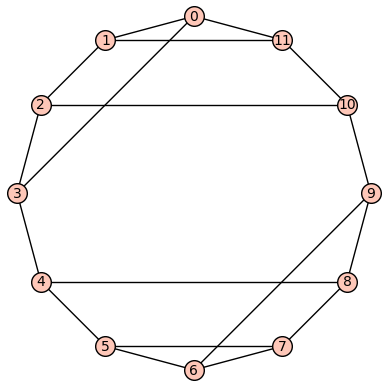
\includegraphics[height=5cm,width=5cm]{graphics/graph_d3reg12e.png}
\end{center}
\begin{center}
%\vspace{8.0 cm}
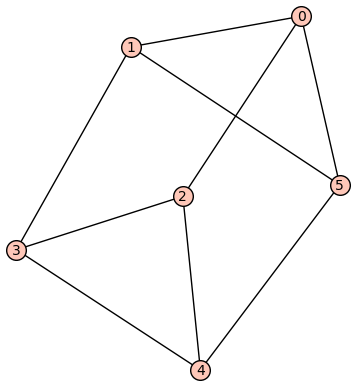
\includegraphics[height=5cm,width=4cm]{graphics/prism6-quotient-of-d3reg12e.png}
\end{center}
\end{minipage}
\caption{The cubic graph  $\Gamma_2$ ({\tt d3reg12e}), with a degree two harmonic quotient morphism to and cover of, the cubic prism graph, $\Gamma_1$.}
\label{fig:harmonic-quotient_d3reg12e+prism6}
\end{figure}

The group
$G = \langle (0,5)(1,7)(2,8)(3,4)(6,11)(9,10) \rangle$ yields the
harmonic quotient morphism (in fact, a quasicover) to the graph
$\Gamma_1 = (V_1,E_1)$, with

\[
V_1=\{0, 1, 2, 3, 4, 5\},
\]
\[
E_1=\{
(0, 1), (0, 5), (1, 2), (1, 3), (2, 4), (2, 5), (3, 4), (4, 5)
\}.
\]
This is tabulated below.

\begin{center}
\begin{tabular}{c|c|c|c}  
  $x$ & $\phi(x)$ & $m_\phi(x)$ & $\nu_\phi(x)$ \\ \hline
  0   &    5   &        1         &  0   \\ 
  1   &    2   &        1         &  0   \\ 
  2   &    1   &        1         &  0   \\ 
  3   &    0   &        1         &  1   \\ 
  4   &    0   &        1         &  1   \\ 
  5   &    5   &        1         &  0    \\ 
  6   &    4   &        1         &  0   \\ 
  7   &    2   &        1         &  0   \\
  8   &    1   &        1         &  0   \\
  9   &    3   &        1         &  1   \\
  10   &   3   &        1         &  1   \\
  11  &    4   &        1         &  0   \\ 
\end{tabular}
\end{center}

\[
  \genus(\Gamma_2) =7,\ \ \ \ \
  \genus(\Gamma_1) =3,
\]

\[
\deg(\phi) =2.
\]

}
\end{example}



\begin{example}% d3reg12f
\label{example:d3reg12f}
  {\tt d3reg12f}\newline
{\rm  
Let $\Gamma_2$ have vertices

\[
V_2=\{0,1,\dots,11\}
\]
and edges

\[
E_2 = \{
(0, 1), (0, 3), (0, 11), (1, 2), (1, 11), (2, 3), (2, 10), (3, 4), (4, 5), (4, 7),
\]
\[
(5, 6), (5, 8), (6, 7), (6, 9), (7, 8), (8, 9), (9, 10), (10, 11)
\}.
\]
This graph has no non-constant harmonic quotient
morphisms $\pi: \Gamma_2\to \Gamma_2/G$, for some subgroup
$G$ of $\Aut(\Gamma_2)$.

}
\end{example}


\begin{example}% d3reg12g
\label{example:d3reg12g}
  {\tt d3reg12g}\newline
{\rm  
Let $\Gamma_2$ have vertices

\[
V_2=\{0,1,\dots,11\}
\]
and edges

\[
E_2 = \{
(0, 1), (0, 4), (0, 11), (1, 2), (1, 3), (2, 3), (2, 5), (3, 4), (4, 5), (5, 6), 
\]
\[
(6, 7), (6, 8), (7, 8), (7, 10), (8, 9), (9, 10), (9, 11), (10, 11)
\}.
\]
This graph has no non-constant harmonic quotient
morphisms $\pi: \Gamma_2\to \Gamma_2/G$, for some subgroup
$G$ of $\Aut(\Gamma_2)$.

}
\end{example}



\begin{example}% d3reg12h
\label{example:d3reg12h}
  {\tt d3reg12h}\newline
{\rm  
Let $\Gamma_2$ have vertices

\[
V_2=\{0,1,\dots,11\}
\]
and edges

\[
E_2 = \{
(0, 1), (0, 3), (0, 11), (1, 2), (1, 4), (2, 3), (2, 5), (3, 4), (4, 5), (5, 6),
\]
\[
 (6, 7), (6, 9), (7, 8), (7, 10), (8, 9), (8, 11), (9, 10), (10, 11)
\}.
\]
This graph has $53$ non-constant harmonic quotient
morphisms $\pi: \Gamma_2\to \Gamma_2/G$, for some subgroup
$G$ of $\Aut(\Gamma_2)$.

Four of these $53$ are distinct non-constant harmonic quotient
morphisms $\pi: \Gamma_2\to \Gamma_2/G=K_{3,3}$, for some subgroup $G$.
(Indeed, these are all covers of this cubic graph.)
%\footnote{One way to visualize the complete bipartite graph $K_{3,3}$
%is to draw $C_6$ and then add ``interior'' edges connecting
%vertices on opposite sides of the circle.}.
\index{complete bipartite graph}
One of these, for the subgroup

\[
G_0=\langle (0,6)(1,7)(2,10)(3,9)(4,8)(5,11) \rangle,
\]
is tabulated below. The uncolored graphs are depicted in
Figure \ref{fig:harmonic-quotient_d3reg12h+K33}.

\begin{center}
\begin{tabular}{c|c|c|c}  
  $x$ & $\phi(x)$ & $m_\phi(x)$ & $\nu_\phi(x)$ \\ \hline
  0   &    3   &        1         &  0   \\ 
  1   &    2   &        1         &  0   \\ 
  2   &    1   &        1         &  0   \\ 
  3   &    4   &        1         &  0   \\ 
  4   &    5   &        1         &  0   \\ 
  5   &    0   &        1         &  0    \\ 
  6   &    3   &        1         &  0   \\ 
  7   &    2   &        1         &  0   \\
  8   &    5   &        1         &  0   \\
  9   &    4   &        1         &  0   \\
  10  &    1   &        1         &  0   \\
  11  &    0   &        1         &  0   \\ 
\end{tabular}
\end{center}

\[
  \genus(\Gamma_2) =7,\ \ \ \ \
  \genus(\Gamma_1) =4,
\]

\[
\deg(\phi) =2.
\]


\begin{figure}[H]
\begin{minipage}{\textwidth}
\begin{center}
%\vspace{8.0 cm}
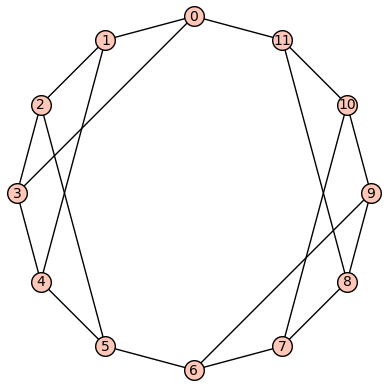
\includegraphics[height=5cm,width=5cm]{graphics/graph_d3reg12h.png}
\end{center}
\begin{center}
%\vspace{8.0 cm}
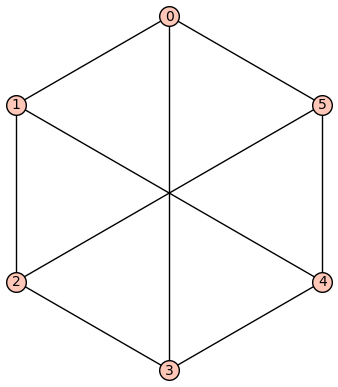
\includegraphics[height=5cm,width=4cm]{graphics/K33-quotient-of-d3reg12h.png}
\end{center}
\end{minipage}
\caption{The cubic graph  $\Gamma_2$ ({\tt d3reg12h}), with a degree two harmonic quotient morphism to and cover of, the complete bipartite graph, $K_{3,3}=\Gamma_2/G_0$.}
\label{fig:harmonic-quotient_d3reg12h+K33}
\end{figure}


Four of the remaining $49$ are distinct non-constant harmonic quotient
morphisms $\pi: \Gamma_2\to \Gamma_2/G=\Gamma_1$, for some $G$.
(Indeed, these are all quasicovers of this
graph\footnote{One way to visualize this graph is to
remove one of the ``interior'' edges of $K_{3,3}$.}
$\Gamma_1$.
One of these quotients, for the subgroup

\[
G_1=\langle (0,11)(1,8)(2,7)(3,10)(4,9)(5,6) \rangle,
\]
is tabulated below. The uncolored graphs are depicted in
Figure \ref{fig:harmonic-quotient_d3reg12h+K33m1}.

\begin{center}
\begin{tabular}{c|c|c|c}  
  $x$ & $\phi(x)$ & $m_\phi(x)$ & $\nu_\phi(x)$ \\ \hline
  0   &    2   &        1         &  1   \\ 
  1   &    0   &        1         &  0   \\ 
  2   &    4   &        1         &  0   \\ 
  3   &    5   &        1         &  0   \\ 
  4   &    3   &        1         &  0   \\ 
  5   &    1   &        1         &  1    \\ 
  6   &    1   &        1         &  1   \\ 
  7   &    4   &        1         &  0   \\
  8   &    0   &        1         &  0   \\
  9   &    3   &        1         &  0   \\
  10  &    5   &        1         &  0   \\
  11  &    2   &        1         &  1   \\ 
\end{tabular}
\end{center}

\[
  \genus(\Gamma_2) =7,\ \ \ \ \
  \genus(\Gamma_1) =3,
\]

\[
\deg(\phi) =2.
\]

\begin{figure}[H]
\begin{minipage}{\textwidth}
\begin{center}
%\vspace{8.0 cm}
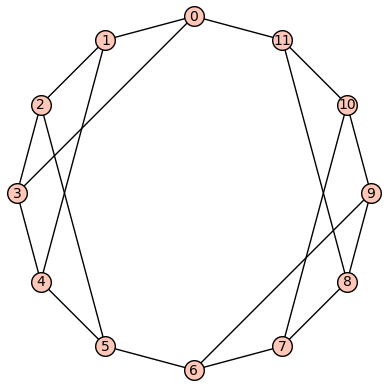
\includegraphics[height=5cm,width=5cm]{graphics/graph_d3reg12h.png}
\end{center}
\begin{center}
%\vspace{8.0 cm}
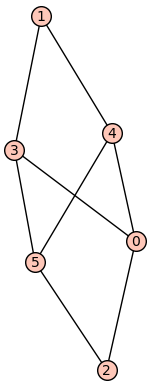
\includegraphics[height=4cm,width=4cm]{graphics/K33m1-quotient-of-d3reg12h.png}
\end{center}
\end{minipage}
\caption{The cubic graph  $\Gamma_2$ ({\tt d3reg12h}), with a degree two harmonic quotient morphism to and quasicover of, $\Gamma_1=\Gamma_2/G_1$.}
\label{fig:harmonic-quotient_d3reg12h+K33m1}
\end{figure}

Four of the remaining $45$ are distinct non-constant harmonic quotient
morphisms $\pi: \Gamma_2\to \Gamma_2/G$, for some $G$, of the barbell
graph, $\Gamma_1=\mathrm{Barbell}(3,0)$.
(Indeed, these are all quasicovers of this graph $\Gamma_1$.)
One of these quotients, for the subgroup
\index{barbell graph}

\[
G_2=\langle (0,5)(1,2)(3,4)(6,11)(7,8)(9,10) \rangle,
\]
is tabulated below. The uncolored graphs are depicted in
Figure \ref{fig:harmonic-quotient_d3reg12h+barbell30}.


\begin{center}
\begin{tabular}{c|c|c|c}  
  $x$ & $\phi(x)$ & $m_\phi(x)$ & $\nu_\phi(x)$ \\ \hline
  0   &    1   &        1         &  0   \\ 
  1   &    3   &        1         &  1   \\ 
  2   &    3   &        1         &  1   \\ 
  3   &    0   &        1         &  1   \\ 
  4   &    0   &        1         &  1   \\ 
  5   &    1   &        1         &  0    \\ 
  6   &    4   &        1         &  0   \\ 
  7   &    5   &        1         &  1   \\
  8   &    5   &        1         &  1   \\
  9   &    2   &        1         &  1   \\
  10  &    2   &        1         &  1   \\
  11  &    4   &        1         &  0   \\ 
\end{tabular}
\end{center}

\[
  \genus(\Gamma_2) =7,\ \ \ \ \
  \genus(\Gamma_1) =2,
\]

\[
\deg(\phi) =2.
\]

\begin{figure}[H]
\begin{minipage}{\textwidth}
\begin{center}
%\vspace{8.0 cm}
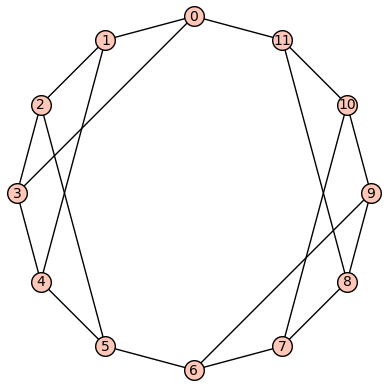
\includegraphics[height=5cm,width=5cm]{graphics/graph_d3reg12h.png}
\end{center}
\begin{center}
%\vspace{8.0 cm}
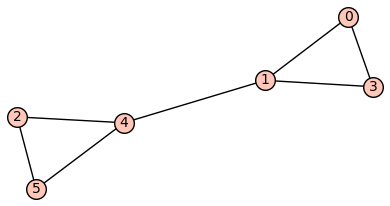
\includegraphics[height=4cm,width=4cm]{graphics/barbell30-quotient-of-d3reg12h.png}
\end{center}
\end{minipage}
\caption{The cubic graph  $\Gamma_2$ ({\tt d3reg12h}), with a degree two harmonic quotient morphism to and quasicover of, $\Gamma_1=\mathrm{Barbell}(3,0)=\Gamma_2/G_2$.}
\label{fig:harmonic-quotient_d3reg12h+barbell30}
\end{figure}

Eight of the remaining $41$ are non-constant harmonic quotient
morphisms $\pi: \Gamma_2\to \Gamma_2/G$, for some $G$, of the
cycle graph, $C_3$.
(Indeed, these are all quasicovers of this graph $\Gamma_1$.)
One of these quotients, for the subgroup\footnote{Note that $G_2\not\subset G_3$. However, the first generator $a$ of $G_3$ generates a subgroup of index $2$ (hence normal) in $G_3$, and $\Gamma_2/\langle a\rangle$ is also isomorphic to $\mathrm{Barbell}(3,0)$. Also note that $C_3$ is a quotient graph of the barbell
graph $\mathrm{Barbell}(3,0)$.}

\[
G_3=\langle (0,5)(1,2)(3,4)(6,11)(7,10)(8,9), (0,11)(1,8)(2,9)(3,10)(4,7)(5,6) \rangle,
\]
is tabulated below. The colored graphs are depicted in
Figure \ref{fig:harmonic-quotient_d3reg12h+C3}.

\begin{center}
\begin{tabular}{c|c|c|c}  
  $x$ & $\phi(x)$ & $m_\phi(x)$ & $\nu_\phi(x)$ \\ \hline
  0   &    1   &        1         &  1   \\ 
  1   &    2   &        1         &  1   \\ 
  2   &    2   &        1         &  1   \\ 
  3   &    0   &        1         &  1   \\ 
  4   &    0   &        1         &  1   \\ 
  5   &    1   &        1         &  1    \\ 
  6   &    1   &        1         &  1   \\ 
  7   &    0   &        1         &  1   \\
  8   &    2   &        1         &  1   \\
  9   &    2   &        1         &  1   \\
  10  &    0   &        1         &  1   \\
  11  &    1   &        1         &  1   \\ 
\end{tabular}
\end{center}

\[
  \genus(\Gamma_2) =7,\ \ \ \ \
  \genus(\Gamma_1) =1,
\]

\[
\deg(\phi) =4.
\]

\begin{figure}[H]
\begin{minipage}{\textwidth}
\begin{center}
%\vspace{8.0 cm}
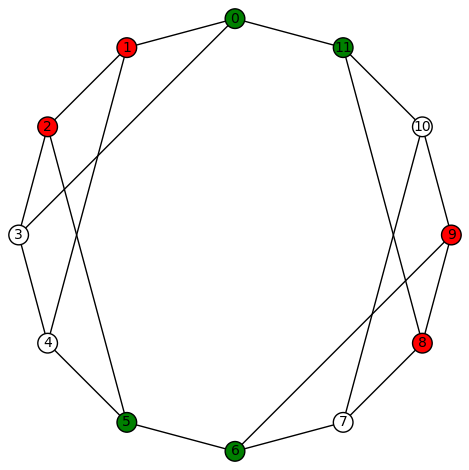
\includegraphics[height=5cm,width=5cm]{graphics/harmonic-quotient_d3reg12h-C3_122001102201.png}
\end{center}
\begin{center}
%\vspace{8.0 cm}
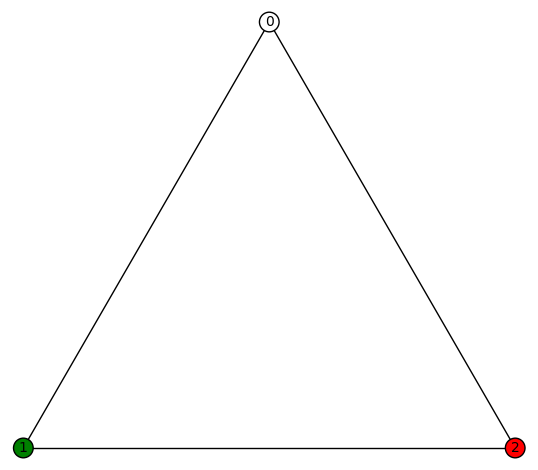
\includegraphics[height=4cm,width=4cm]{graphics/cycle3-012.png}
\end{center}
\end{minipage}
\caption{The cubic graph  $\Gamma_2$ ({\tt d3reg12h}), with a degree four harmonic quotient morphism to and quasicover of, $\Gamma_1=C_3=\Gamma_2/G_3$.}
\label{fig:harmonic-quotient_d3reg12h+C3}
\end{figure}

The remaining $33$ (one of which is $G=\Aut(\Gamma_2)$) all give the same
harmonic quotient morphism, to $P_2$.

}
\end{example}



\begin{example}% d3reg12i
\label{example:d3reg12i}
  {\tt d3reg12i}\newline
{\rm  
Let $\Gamma_2$ have vertices

\[
V_2=\{0,1,\dots,11\}
\]
and edges

\[
E_2 = \{
(0, 1), (0, 2), (0, 11), (1, 2), (1, 10), (2, 3), (3, 4), (3, 6), (4, 5),
\]
\[
(4, 7), (5, 6), (5, 8), (6, 7), (7, 8), (8, 9), (9, 10), (9, 11), (10, 11)
\}.
\]
This graph has $2$ non-constant harmonic quotient
morphisms $\pi: \Gamma_2\to \Gamma_2/G$, for some subgroup
$G$ of $\Aut(\Gamma_2)$. Both are distinct non-constant harmonic quotient
morphisms $\pi: \Gamma_2\to \Gamma_2/G$, for some $G$, of the barbell
graph, $\Gamma_1=\mathrm{Barbell}(3,0)$.
\index{barbell graph}
(Indeed, these are all quasicovers of this graph $\Gamma_1$.)
One of these quotients, for the subgroup

\[
G_2=\langle (0,11)(1,10)(2,9)(3,8)(4,5)(6,7) \rangle,
\]
is tabulated below.
\begin{center}
\begin{tabular}{c|c|c|c}  
  $x$ & $\phi(x)$ & $m_\phi(x)$ & $\nu_\phi(x)$ \\ \hline
  0   &    1   &        1         &  1   \\ 
  1   &    4   &        1         &  1   \\ 
  2   &    5   &        1         &  0   \\ 
  3   &    0   &        1         &  0   \\ 
  4   &    2   &        1         &  1   \\ 
  5   &    2   &        1         &  1    \\ 
  6   &    3   &        1         &  1   \\ 
  7   &    3   &        1         &  1   \\
  8   &    0   &        1         &  0   \\
  9   &    5   &        1         &  0   \\
  10  &    4   &        1         &  1   \\
  11  &    1   &        1         &  1   \\ 
\end{tabular}
\end{center}

\[
  \genus(\Gamma_2) =7,\ \ \ \ \
  \genus(\Gamma_1) =2,
\]

\[
\deg(\phi) =2.
\]

}
\end{example}



\begin{example}% d3reg12j
\label{example:d3reg12j}
  {\tt d3reg12j}\newline
{\rm  
Let $\Gamma_2$ have vertices

\[
V_2=\{0,1,\dots,11\}
\]
and edges

\[
E_2 = \{
(0, 1), (0, 2), (0, 11), (1, 2), (1, 4), (2, 3), (3, 4), (3, 5), (4, 5),
\]
\[
(5, 6), (6, 7), (6, 8), (7, 8), (7, 10), (8, 9), (9, 10), (9, 11), (10, 11)
\}.
\]
This graph has $15$ non-constant harmonic quotient
morphisms $\pi: \Gamma_2\to \Gamma_2/G$, for some subgroup
$G$ of $\Aut(\Gamma_2)$.

Two of these are distinct non-constant harmonic quotient
morphisms $\pi: \Gamma_2\to \Gamma_2/G$, for some $G$, of
the (cubic) prism graph (in fact, both a
degree $2$ covers).
\index{prism graph}
One of these quotients, for the subgroup

\[
G_2=\langle (0,6)(1,7)(2,8)(3,9)(4,10)(5,11) \rangle,
\]
is tabulated below.
\begin{center}
\begin{tabular}{c|c|c|c}  
  $x$ & $\phi(x)$ & $m_\phi(x)$ & $\nu_\phi(x)$ \\ \hline
  0   &    4   &        1         &  0   \\ 
  1   &    3   &        1         &  0   \\ 
  2   &    1   &        1         &  0   \\ 
  3   &    5   &        1         &  0   \\ 
  4   &    0   &        1         &  0   \\ 
  5   &    2   &        1         &  0    \\ 
  6   &    4   &        1         &  0   \\ 
  7   &    3   &        1         &  0   \\
  8   &    1   &        1         &  0   \\
  9   &    5   &        1         &  0   \\
  10  &    0   &        1         &  0   \\
  11  &    2   &        1         &  0   \\ 
\end{tabular}
\end{center}

\[
  \genus(\Gamma_2) =7,\ \ \ \ \
  \genus(\Gamma_1) =4,
\]

\[
\deg(\phi) =2.
\]


One of the remaining $13$ is a non-constant harmonic quotient
morphism $\pi: \Gamma_2\to \Gamma_2/G$, for some $G$,
for the barbell
graph, $\Gamma_1=\mathrm{Barbell}(3,0)$.
\index{barbell graph}
This quotient, for the subgroup

\[
G=\langle  (0,5)(1,4)(2,3)(6,11)(7,10)(8,9) \rangle,
\]
is tabulated below.
\begin{center}
\begin{tabular}{c|c|c|c}  
  $x$ & $\phi(x)$ & $m_\phi(x)$ & $\nu_\phi(x)$ \\ \hline
  0   &    5   &        1         &  0   \\ 
  1   &    0   &        1         &  1   \\ 
  2   &    1   &        1         &  1   \\ 
  3   &    1   &        1         &  1   \\ 
  4   &    0   &        1         &  1   \\ 
  5   &    5   &        1         &  0    \\ 
  6   &    4   &        1         &  0   \\ 
  7   &    2   &        1         &  1   \\
  8   &    3   &        1         &  1   \\
  9   &    3   &        1         &  1   \\
  10  &    2   &        1         &  1   \\
  11  &    4   &        1         &  0   \\ 
\end{tabular}
\end{center}

\[
  \genus(\Gamma_2) =7,\ \ \ \ \
  \genus(\Gamma_1) =2,
\]

\[
\deg(\phi) =2.
\]

Two of the remaining $12$ are distinct non-constant harmonic quotient
morphisms $\pi: \Gamma_2\to \Gamma_2/G$, for some $G$, of
codomino graph.
\index{codomino graph}
One of these quotients, for the subgroup

\[
G=\langle (0,11)(1,9)(2,10)(3,7)(4,8)(5,6) \rangle,
\]
is tabulated below. The uncolored graphs are depicted in
Figure \ref{fig:harmonic-quotient_d3reg12j+codomino}.

\begin{center}
\begin{tabular}{c|c|c|c}  
  $x$ & $\phi(x)$ & $m_\phi(x)$ & $\nu_\phi(x)$ \\ \hline
  0   &    3   &        1         &  1   \\ 
  1   &    1   &        1         &  0  \\ 
  2   &    2   &        1         &  0  \\ 
  3   &    4   &        1         &  0  \\ 
  4   &    5   &        1         &  0   \\ 
  5   &    0   &        1         &  1    \\ 
  6   &    0   &        1         &  1   \\ 
  7   &    4   &        1         &  0   \\
  8   &    5   &        1         &  0   \\
  9   &    1   &        1         &  0   \\
  10  &    2   &        1         &  0   \\
  11  &    3   &        1         &  1   \\ 
\end{tabular}
\end{center}

\[
  \genus(\Gamma_2) =7,\ \ \ \ \
  \genus(\Gamma_1) =3,
\]

\[
\deg(\phi) =2.
\]

\begin{figure}[H]
\begin{minipage}{\textwidth}
\begin{center}
%\vspace{8.0 cm}
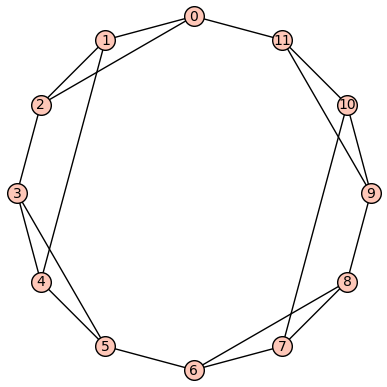
\includegraphics[height=5cm,width=5cm]{graphics/graph_d3reg12j.png}
\end{center}
\begin{center}
%\vspace{8.0 cm}
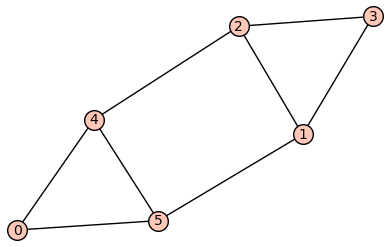
\includegraphics[height=4cm,width=4cm]{graphics/codomino-quotient-of-d3reg12j.png}
\end{center}
\end{minipage}
\caption{The cubic graph  $\Gamma_2$ ({\tt d3reg12j}), with a degree two harmonic quotient morphism to and quasicover of the codomino graph, $\Gamma_1=\Gamma_2/G_2$.}
\label{fig:harmonic-quotient_d3reg12j+codomino}
\end{figure}

We tabulate the subgroups and their (harmonic) quotients
$\Gamma_1=\Gamma_2/G$. 

{\small{
\begin{center}
\begin{tabular}{c|c}
  gens of $G\subset \Aut(\Gamma_2)$ & $\Gamma_2/G$ \\ \hline
  (0,6)(1,7)(2,8)(3,9)(4,10)(5,11) & prism \\ \hline
  (0,6)(1,8)(2,7)(3,10)(4,9)(5,11) & prism \\ \hline
  (0,5)(1,4)(2,3)(6,11)(7,10)(8,9) & $\mathrm{Barbell}(3,0)$ \\ \hline
  (0,11)(1,9)(2,10)(3,7)(4,8)(5,6) & codomino \\ \hline
  (0,11)(1,10)(2,9)(3,8)(4,7)(5,6) & codomino \\ \hline
  (0,5)(1,4)(2,3)(6,11)(7,10)(8,9), & \\
  (0,6)(1,7)(2,8)(3,9)(4,10)(5,11) & $C_3$ \\ \hline
  (0,5)(1,4)(2,3)(6,11)(7,10)(8,9), & \\
  (0,6)(1,8)(2,7)(3,10)(4,9)(5,11)  & $C_3$ \\ \hline
(1,2)(3,4)(7,8)(9,10), & \\
(0,11)(1,10,2,9)(3,8,4,7)(5,6)  & $P_4$ \\ \hline
  (1,2)(3,4)(7,8)(9,10), & \\
  (0,11)(1,9)(2,10)(3,7)(4,8)(5,6)  & $P_4$ \\ \hline
  (7,8)(9,10), (1,2)(3,4), & \\
  (0,11)(1,9)(2,10)(3,7)(4,8)(5,6)  & $P_4$ \\ \hline
  (1,2)(3,4)(7,8)(9,10),  & \\
  (0,5)(1,3)(2,4)(6,11)(7,9)(8,10), & \\
  (0,6)(1,7)(2,8)(3,9)(4,10)(5,11) & $P_2$ \\ \hline
  (1,2)(3,4)(7,8)(9,10), & \\
  (0,5)(1,3)(2,4)(6,11)(7,10)(8,9), & \\
  (0,6)(1,7)(2,8)(3,9)(4,10)(5,11) & $P_2$ \\ \hline
  (1,2)(3,4)(7,8)(9,10), & \\
  (0,5)(1,3)(2,4)(6,11)(7,9)(8,10), & \\
  (0,6)(1,8,2,7)(3,10,4,9)(5,11) & $P_2$ \\ \hline
  (1,2)(3,4)(7,8)(9,10), & \\
  (0,5)(1,3)(2,4)(6,11)(7,10)(8,9), & \\
  (0,6)(1,8,2,7)(3,10,4,9)(5,11) & $P_2$ \\
\end{tabular}
\end{center}
}}
The table omits one subgroup, $G=\Aut(\Gamma_2)$ itself, whose quotient is
also $P_2$. All the quotient morphisms to $P_4$ in the above table are the same,
and all those to $P_2$ are the same.

Using this table one can see that

(a) One of the quotient morphisms to the prism graph has a further
quotient to $C_3$.

(b) One of the quotient morphisms to the codomino graph has a further
quotient to $P_4$.

(c) One of the quotient morphisms to the barbell graph has a further
quotient to $C_3$.
}
\end{example}



\begin{example}% d3reg12k
\label{example:d3reg12k}
  {\tt d3reg12k}\newline
{\rm  
Let $\Gamma_2$ have vertices

\[
V_2=\{0,1,\dots,11\}
\]
and edges

\[
E_2 = \{
(0, 1), (0, 10), (0, 11), (1, 2), (1, 4), (2, 3), (2, 8), (3, 4), (3, 6),
\]
\[
(4, 5), (5, 6), (5, 7), (6, 7), (7, 8), (8, 9), (9, 10), (9, 11), (10, 11)
\}.
\]
This graph has no non-constant harmonic quotient
morphisms $\pi: \Gamma_2\to \Gamma_2/G$, for some subgroup
$G$ of $\Aut(\Gamma_2)$.

}
\end{example}


\begin{example}% d3reg12l
\label{example:d3reg12l}
  {\tt d3reg12l}\newline
{\rm  
Let $\Gamma_2$ have vertices

\[
V_2=\{0,1,\dots,11\}
\]
and edges

\[
E_2 = \{
(0, 1), (0, 6), (0, 11), (1, 2), (1, 11), (2, 3), (2, 4), (3, 4), (3, 9),
\]
\[
(4, 5), (5, 6), (5, 7), (6, 7), (7, 8), (8, 9), (8, 10), (9, 10), (10, 11)
\}.
\]
This graph has $10$ non-constant harmonic quotient
morphisms $\pi: \Gamma_2\to \Gamma_2/G$, for some subgroup
$G$ of $\Aut(\Gamma_2)$.

Three of these $10$ are distinct non-constant harmonic quotient
morphisms $\pi: \Gamma_2\to \Gamma_2/G$, for some $G$, of
codomino graph.
\index{codomino graph}
One of these quotients, for the subgroup

\[
G_1=\langle (0,3)(1,2)(4,11)(5,10)(6,9)(7,8) \rangle,
\]
is tabulated below.

\begin{center}
\begin{tabular}{c|c|c|c}  
  $x$ & $\phi(x)$ & $m_\phi(x)$ & $\nu_\phi(x)$ \\ \hline
  0   &    4   &        1         &  0   \\ 
  1   &    3   &        1         &  1  \\ 
  2   &    3   &        1         &  1  \\ 
  3   &    4   &        1         &  0  \\ 
  4   &    1   &        1         &  0   \\ 
  5   &    2   &        1         &  0    \\ 
  6   &    0   &        1         &  0   \\ 
  7   &    5   &        1         &  1   \\
  8   &    5   &        1         &  1   \\
  9   &    0   &        1         &  0   \\
  10  &    2   &        1         &  0   \\
  11  &    1   &        1         &  0   \\ 
\end{tabular}
\end{center}

\[
  \genus(\Gamma_2) =7,\ \ \ \ \
  \genus(\Gamma_1) =3,
\]

\[
\deg(\phi) =2.
\]

One of the remaining $7$ is a distinct non-constant harmonic quotient
morphism $\pi: \Gamma_2\to \Gamma_2/G$, for some $G$, of
cycle graph, $C_3$.
The quotient $\phi: \Gamma_2\to \Gamma_2/G_2$ for the subgroup

\[
G_2=\langle (0,3)(1,2)(4,11)(5,10)(6,9)(7,8),
(0,6)(1,7)(2,8)(3,9)(4,10)(5,11) \rangle,
\]
is tabulated below. Note that $G_1$ is a (normal) subgroup of $G_2$.
We conclude that one of the quotient morphisms to the
codomino graph has a further quotient to $C_3$.

\begin{center}
\begin{tabular}{c|c|c|c}  
  $x$ & $\phi(x)$ & $m_\phi(x)$ & $\nu_\phi(x)$ \\ \hline
  0   &    2   &        1         &  1   \\ 
  1   &    1   &        1         &  1  \\ 
  2   &    1   &        1         &  1  \\ 
  3   &    2   &        1         &  1  \\ 
  4   &    0   &        1         &  1   \\ 
  5   &    0   &        1         &  1    \\ 
  6   &    2   &        1         &  1   \\ 
  7   &    1   &        1         &  1   \\
  8   &    1   &        1         &  1   \\
  9   &    2   &        1         &  1   \\
  10  &    0   &        1         &  1   \\
  11  &    0   &        1         &  1   \\ 
\end{tabular}
\end{center}

\[
  \genus(\Gamma_2) =7,\ \ \ \ \
  \genus(\Gamma_1) =1,
\]

\[
\deg(\phi) =4.
\]

Three of the remaining $6$ are distinct non-constant harmonic quotient
morphisms $\pi: \Gamma_2\to \Gamma_2/G$, for some $G$, of
the path graph, $P_4$.
The remaining $3$ are distinct non-constant harmonic quotient
morphisms $\pi: \Gamma_2\to \Gamma_2/G$, for some $G$, of
the path graph, $P_2$.

}
\end{example}




\begin{example}% d3reg12m
\label{example:d3reg12m}
  {\tt d3reg12m}\newline
{\rm  
Let $\Gamma_2$ have vertices

\[
V_2=\{0,1,\dots,11\}
\]
and edges

\[
E_2 = \{
(0, 1), (0, 9), (0, 11), (1, 2), (1, 4), (2, 3), (2, 11), (3, 4), (3, 6),
\]
\[
(4, 5), (5, 6), (5, 8), (6, 7), (7, 8), (7, 10), (8, 9), (9, 10), (10, 11)
\}.
\]
This graph has $31$ non-constant harmonic quotient
morphisms $\pi: \Gamma_2\to \Gamma_2/G$, for some subgroup
$G$ of $\Aut(\Gamma_2)$.

Three of these $31$ are distinct non-constant harmonic quotient
morphisms $\pi: \Gamma_2\to \Gamma_2/G$, for some $G$, of
codomino graph.
\index{codomino graph}

Three of the remaining $28$ are distinct non-constant harmonic quotient
morphisms $\pi: \Gamma_2\to \Gamma_2/G$, for some $G$, of
grid graph $P_2\times P_3$ (the $2\times 3$ grid, or domino graph).
\index{grid graph}

One of the remaining $25$ is a distinct non-constant harmonic quotient
morphism $\pi: \Gamma_2\to \Gamma_2/G$, for some $G$, of
complete bipartite graph, $K_{3,3}$.

One of the remaining $24$ is a distinct non-constant harmonic quotient
morphism $\pi: \Gamma_2\to \Gamma_2/G$, for some $G$, of
(cubic) prism graph.
\index{prism graph}

One of the remaining $23$ is a distinct non-constant harmonic quotient
morphism $\pi: \Gamma_2\to \Gamma_2/G$, for some $G$, of
cycle graph, $C_6$.
The quotient $\phi: \Gamma_2\to \Gamma_2/G$ for the subgroup

\[
G=\langle (0,11)(1,2)(3,4)(5,6)(7,8)(9,10) \rangle,
\]
is tabulated below. 

\begin{center}
\begin{tabular}{c|c|c|c}  
  $x$ & $\phi(x)$ & $m_\phi(x)$ & $\nu_\phi(x)$ \\ \hline
  0   &    2   &        1         &  1   \\ 
  1   &    4   &        1         &  1  \\ 
  2   &    4   &        1         &  1  \\ 
  3   &    0   &        1         &  1  \\ 
  4   &    0   &        1         &  1   \\ 
  5   &    1   &        1         &  1    \\ 
  6   &    1   &        1         &  1   \\ 
  7   &    5   &        1         &  1   \\
  8   &    5   &        1         &  1   \\
  9   &    3   &        1         &  1   \\
  10  &    3   &        1         &  1   \\
  11  &    2   &        1         &  1   \\ 
\end{tabular}
\end{center}

\[
  \genus(\Gamma_2) =7,\ \ \ \ \
  \genus(\Gamma_1) =1,
\]

\[
\deg(\phi) =2.
\]

Three of the remaining $22$ are distinct non-constant harmonic quotient
morphisms $\pi: \Gamma_2\to \Gamma_2/G$, for some $G$, of
path graph, $P_4$.

Four of the remaining $19$ are distinct non-constant harmonic quotient
morphisms $\pi: \Gamma_2\to \Gamma_2/G$, for some $G$, of
cycle graph, $C_3$.

Three of the remaining $15$ are distinct non-constant harmonic quotient
morphisms $\pi: \Gamma_2\to \Gamma_2/G$, for some $G$, of
path graph, $P_3$.

The remaining $12$ are (not necessarily distinct) non-constant harmonic quotient
morphisms $\pi: \Gamma_2\to \Gamma_2/G$, for some $G$, of
path graph, $P_2$.


}
\end{example}



\begin{example}% d3reg12n
\label{example:d3reg12n}
  {\tt d3reg12n}\newline
{\rm  
Let $\Gamma_2$ be the Franklin graph, with vertices
\index{Franklin graph}

\[
V_2=\{0,1,\dots,11\}
\]
and edges

\[
E_2 = \{
(0, 1), (0, 5), (0, 6), (1, 2), (1, 7), (2, 3), (2, 8), (3, 4), (3, 9), (4, 5), 
\]
\[
(4, 10), (5, 11), (6, 7), (6, 9), (7, 10), (8, 9), (8, 11), (10, 11)
\}.
\]
This graph has $35$ non-constant harmonic quotient
morphisms $\pi: \Gamma_2\to \Gamma_2/G$, for some subgroup
$G$ of $\Aut(\Gamma_2)$.

Six of these $35$ are distinct non-constant harmonic quotient
morphisms $\pi: \Gamma_2\to \Gamma_2/G$, for some $G$,  to
the {\tt EUYo}
co-twin-$C_5$ graph\footnote{We are using the naming conventions
of graph6 \cite{Mc26}. In the ISGCI it is the co-twin-$C_5$ graph
\cite{dR26}.}.
\index{co-twin-$C_5$ graph}
One of these quotients, for the subgroup

\[
G=\langle (0,1)(2,5)(3,11)(4,8)(6,7)(9,10) \rangle,
\]
is tabulated below. The uncolored graphs are depicted in
Figure \ref{fig:harmonic-quotient_d3reg12n+cotwinC5}.

\begin{center}
\begin{tabular}{c|c|c|c}  
  $x$ & $\phi(x)$ & $m_\phi(x)$ & $\nu_\phi(x)$ \\ \hline
  0   &    1   &        1         &  1   \\ 
  1   &    1   &        1         &  1  \\ 
  2   &    4   &        1         &  0  \\ 
  3   &    3   &        1         &  0  \\ 
  4   &    5   &        1         &  0   \\ 
  5   &    4   &        1         &  0  \\ 
  6   &    2   &        1         &  1   \\ 
  7   &    2   &        1         &  1   \\
  8   &    5   &        1         &  0   \\
  9   &    0   &        1         &  0   \\
  10  &    0   &        1         &  0   \\
  11  &    3   &        1         &  0   \\ 
\end{tabular}
\end{center}

\[
  \genus(\Gamma_2) =7,\ \ \ \ \
  \genus(\Gamma_1) =3,
\]

\[
\deg(\phi) =2.
\]

\begin{figure}[H]
\begin{minipage}{\textwidth}
\begin{center}
%\vspace{8.0 cm}
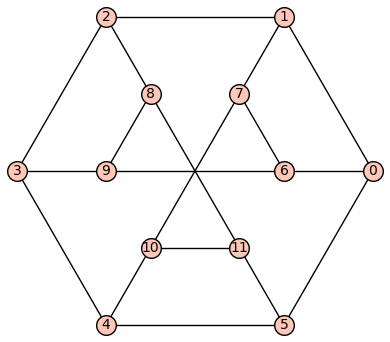
\includegraphics[height=5cm,width=5cm]{graphics/graph_d3reg12n.png}
\end{center}
\begin{center}
%\vspace{8.0 cm}
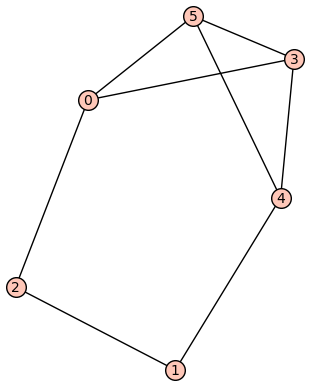
\includegraphics[height=4cm,width=4cm]{graphics/cotwinC5-quotient-of-d3reg12n.png}
\end{center}
\end{minipage}
\caption{The cubic graph  $\Gamma_2$ ({\tt d3reg12n}), with a degree two harmonic quotient morphism to and quasicover of the co-twin-$C_5$ graph, $\Gamma_1=\Gamma_2/G$.}
\label{fig:harmonic-quotient_d3reg12n+cotwinC5}
\end{figure}

One of the remaining $29$ is a distinct non-constant harmonic quotient
morphism $\pi: \Gamma_2\to \Gamma_2/G$, for some $G$, of
the $X_{37}$ graph (see Remark~\ref{rem:x37}).
\index{$X_{37}$ graph}
One of these quotients, for the subgroup

\[
G=\langle (0,1)(2,5)(3,4)(6,7)(8,11)(9,10) \rangle,
\]
is tabulated below. The uncolored graphs are depicted in
Figure \ref{fig:harmonic-quotient_d3reg12n+X37}.

\begin{center}
\begin{tabular}{c|c|c|c}  
  $x$ & $\phi(x)$ & $m_\phi(x)$ & $\nu_\phi(x)$ \\ \hline
  0   &    4   &        1         &  1   \\ 
  1   &    4   &        1         &  1  \\ 
  2   &    5   &        1         &  0  \\ 
  3   &    0   &        1         &  1  \\ 
  4   &    0   &        1         &  1   \\ 
  5   &    5   &        1         &  0  \\ 
  6   &    1   &        1         &  1   \\ 
  7   &    1   &        1         &  1   \\
  8   &    2   &        1         &  1   \\
  9   &    3   &        1         &  0   \\
  10  &    3   &        1         &  0   \\
  11  &    2   &        1         &  1   \\ 
\end{tabular}
\end{center}

\[
  \genus(\Gamma_2) =7,\ \ \ \ \
  \genus(\Gamma_1) =2,
\]

\[
\deg(\phi) =2.
\]

\begin{figure}[H]
\begin{minipage}{\textwidth}
\begin{center}
%\vspace{8.0 cm}
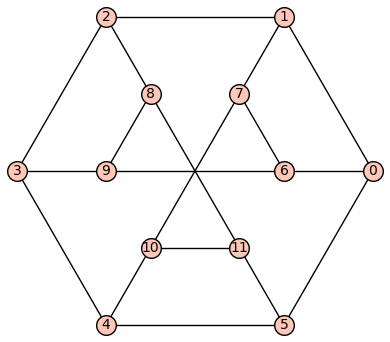
\includegraphics[height=5cm,width=5cm]{graphics/graph_d3reg12n.png}
\end{center}
\begin{center}
%\vspace{8.0 cm}
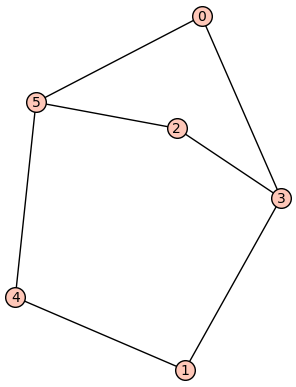
\includegraphics[height=4cm,width=4cm]{graphics/X37-quotient-of-d3reg12n.png}
\end{center}
\end{minipage}
\caption{The cubic graph  $\Gamma_2$ ({\tt d3reg12n}), with a degree two harmonic quotient morphism to and quasicover of the $X_{37}$ graph, $\Gamma_1=\Gamma_2/G_2$.}
\label{fig:harmonic-quotient_d3reg12n+X37}
\end{figure}

\begin{revremark}
\label{rem:x37}
The ISGCI name $X_{37}$ was not checked in 2026. The quotient graph of this
paragraph is isomorphic to the twin-$C_5$ graph of the next paragraph. So
the six quotients described in the two paragraphs all have the same
isomorphism type.
\end{revremark}


Five of the remaining $28$ are distinct non-constant harmonic quotient
morphisms $\pi: \Gamma_2\to \Gamma_2/G$, for some $G$, of
twin-$C_5$ graph.
\index{twin-$C_5$ graph}
One of these quotients, for the subgroup

\[
G=\langle (0,3)(1,2)(4,5)(6,9)(7,8)(10,11) \rangle,
\]
is tabulated below. The uncolored graphs are depicted in
Figure \ref{fig:harmonic-quotient_d3reg12n+twinC5}.

\begin{center}
\begin{tabular}{c|c|c|c}  
  $x$ & $\phi(x)$ & $m_\phi(x)$ & $\nu_\phi(x)$ \\ \hline
  0   &    2   &        1         &  0   \\ 
  1   &    1   &        1         &  1  \\ 
  2   &    1   &        1         &  1  \\ 
  3   &    2   &        1         &  0  \\ 
  4   &    3   &        1         &  1   \\ 
  5   &    3   &        1         &  1  \\ 
  6   &    0   &        1         &  1   \\ 
  7   &    5   &        1         &  0   \\
  8   &    5   &        1         &  0   \\
  9   &    0   &        1         &  1   \\
  10  &    4   &        1         &  1   \\
  11  &    4   &        1         &  1   \\ 
\end{tabular}
\end{center}

\[
  \genus(\Gamma_2) =7,\ \ \ \ \
  \genus(\Gamma_1) =2,
\]

\[
\deg(\phi) =2.
\]

\begin{figure}[H]
\begin{minipage}{\textwidth}
\begin{center}
%\vspace{8.0 cm}
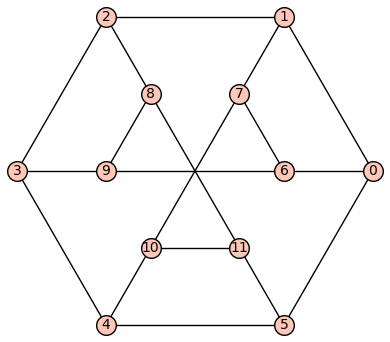
\includegraphics[height=5cm,width=5cm]{graphics/graph_d3reg12n.png}
\end{center}
\begin{center}
%\vspace{8.0 cm}
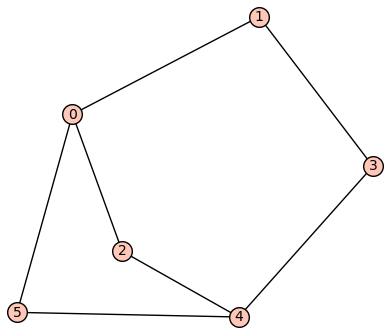
\includegraphics[height=4cm,width=4cm]{graphics/twinC5b-quotient-of-d3reg12n.png}
\end{center}
\end{minipage}
\caption{The cubic graph  $\Gamma_2$ ({\tt d3reg12n}), with a degree two harmonic quotient morphism to and quasicover of the twin-$C_5$ graph, $\Gamma_1=\Gamma_2/G_2$.}
\label{fig:harmonic-quotient_d3reg12n+twinC5}
\end{figure}

Nine of the remaining $23$ are (not necessarily distinct)
non-constant harmonic quotient
morphism $\pi: \Gamma_2\to \Gamma_2/G$, for some $G$, of
the star graph $St_4$ having $4$ vertices.
\index{star graph}

All of the remaining $14$ are (not necessarily distinct)
non-constant harmonic quotient
morphism $\pi: \Gamma_2\to \Gamma_2/G$, for some $G$, of
the path graph $P_2$.
}
\end{example}



\section{Quartic cases}
\label{sec:quartic-examples}

This section treats connected quartic graphs with $5$ to $12$ vertices.
For $9$ or more vertices only a selection of the graphs is included.
Each subsection lists the graphs and then works out harmonic quotients
in a series of examples.


\subsection{\texorpdfstring{$5$}{5} vertices}

This subsection describes the connected quartic graphs on $5$ vertices.
It records their invariants and harmonic morphism counts, and then
works out harmonic quotient morphisms in examples.


The complete graph $K_5$ is the only quartic graph on $5$ vertices.

Since a non-trivial harmonic morphism is surjective on the vertices and
since it sends neighbors to neighbors, there can be no non-trivial
harmonic morphism from $K_5$ (or any complete graph) to
$St_4$, $P_4$, or to $C_4$.
%By Theorem \ref{thm:harm-morphism-complete},
By general theory, we know
the number of non-trivial harmonic morphisms to $K_3=C_3$ or to $K_4$ is $0$. 


\subsubsection{Examples}

Each example below takes one graph from the list above and describes
its harmonic quotient morphisms.


\begin{example}% d4reg5a
\label{example:d4reg5a}
  {\tt d4reg5a}\newline
{\rm  
  Let $\Gamma_2=K_5$, in standard form.

There are $75$ harmonic quotient morphisms
$\pi: \Gamma_2\to \Gamma_1=\Gamma_2/G$,
for some $G$, but most are not distinct. Every quotient is
$\Gamma_1=P_2$, and there are no others.
An example for
\[
G = \langle (1,3)(2,4), (1,4)(2,3)\rangle
\]
is tabulated below.

\begin{center}
\begin{tabular}{c|c|c|c}  
  $x$ & $\phi(x)$ & $m_\phi(x)$ & $\nu_\phi(x)$ \\ \hline
  0   &    1   &        4         &  0   \\ 
  1   &    0   &        1         &  3  \\ 
  2   &    0   &        1         &  3  \\ 
  3   &    0   &        1         &  3  \\ 
  4   &    0   &        1         &  3   \\ 
\end{tabular}
\end{center}

\[
  \genus(\Gamma_2) =6,\ \ \ \ \
  \genus(\Gamma_1) =0,
\]

\[
\deg(\phi) =4.
\]
}
\end{example}


\subsection{\texorpdfstring{$6$}{6} vertices}

This subsection describes the connected quartic graphs on $6$ vertices.
It records their invariants and harmonic morphism counts, and then
works out harmonic quotient morphisms in examples.


There is (up to isomorphism) exactly one $4$-regular connected graph
on $6$ vertices, the octahedral graph (also known as $K_{2,2,2}$).
\index{octahedral graph}

Define $\Gamma=(V,E)$ to have vertices $V=$
% d4reg6a

\[
V = \{0,1,2,3,4,5\},
\]
and edges $E=$
\[
\{(0, 1), (0, 2), (0, 4), (0, 5), (1, 2), (1, 3), (1, 4), (2, 3), (2, 5), (3, 4), (3, 5), (4, 5)\}.
\]
It is an integral graph\footnote{The multiset of eigenvalues of
  the adjacency matrix is $\{4, 0, 0, 0, -2, -2\}$.} with girth $3$,
diameter $2$, and circumference $6$ (i.e., is a
Hamiltonian graph).
\index{integral graph}
Its automorphism group is order $48$ and it's vertex transitive,
edge transitive, strongly regular, and distance regular.
The size of the critical group of this graph is $384=2^73$.
\index{vertex transitive graph}
\index{edge transitive graph}
\index{distance regular graph}
\index{strongly regular graph}

There are no non-trivial harmonic morphisms to $St_4$, $P_4$, $C_4$,
or to $K_4$.
There are exactly $6$ non-trivial harmonic morphisms $\Gamma\to P_3$ and
$6$ non-trivial harmonic
morphisms\footnote{All $6$ of these morphisms to $C_3$ are
  $2$-multicovers of degree $4$.} $\Gamma\to C_3$.



\subsubsection{Examples}

Each example below takes one graph from the list above and describes
its harmonic quotient morphisms.


\begin{example}% d4reg6a
\label{example:d4reg6a}
 {\tt d4reg6a}\newline
{\rm  
  Let $\Gamma_2$ denote the octahedral graph as given above.
There are $59$ harmonic quotient morphisms
$\pi: \Gamma_2\to \Gamma_1=\Gamma_2/G$,
for some $G$, but most are not distinct.

Six of these $59$ are distinct harmonic quotient morphisms
to the diamond graph.

Of the remaining $53$, $6$ are
harmonic quotient morphisms to the cycle graph $C_3$ (all six give the same
morphism). As we
know from the paragraph above, all of these morphisms to $C_3$ are
$2$-multicovers. Another $9$ are harmonic quotient morphisms to $P_3$
($3$ distinct morphisms).

The remaining $38$ are (not necessarily distinct)
harmonic quotient morphisms to the path graph $P_2$.
}
\end{example}



\subsection{\texorpdfstring{$7$}{7} vertices}

This subsection describes the connected quartic graphs on $7$ vertices.
It records their invariants and harmonic morphism counts, and then
works out harmonic quotient morphisms in examples.


There are (up to isomorphism) exactly two $4$-regular connected graphs on $7$ vertices.

\begin{enumerate}
\item
  {\tt d4reg7a}
Define $\Gamma=(V,E)$ to have vertex vertex set $\{0,1,2,3,4,5,6\}$ and edge set:

\[
\{(0, 1), (0, 3), (0, 5), (0, 6), (1, 2), (1, 3), (1, 5), (2, 3), (2, 4),
\]
\[
(2, 6), (3, 4), (4, 5), (4, 6), (5, 6)\}.
\]
It has girth $3$, diameter $2$, and is a
Hamiltonian graph (with circumference $7$).
Its automorphism group is order $14$ and acts transitively on the vertices
(but it's not edge transitive).
The size of the critical group of this graph is $1183=7\cdot 13^2$.

There are no non-trivial harmonic morphisms to $St_4$, $P_3$, $P_4$, $C_3$, $C_4$ or to $K_4$.

\item
{\tt d4reg7b}
Define $\Gamma=(V,E)$ to have vertex vertex set $\{0,1,2,3,4,5,6\}$ and edge set:

\[
\{
(0, 1), (0, 3), (0, 4), (0, 6), (1, 2), (1, 5), (1, 6), (2, 3), (2, 4),
\]
\[
(2, 6), (3, 4), (3, 5), (4, 5), (5, 6)
\}.
\]
It has girth $3$, diameter $2$, and is a
Hamiltonian graph (with circumference $7$).
Its automorphism group is order $48$ and it does not act transitively on the vertices.
The size of the critical group of this graph is $1200=2^43\cdot 5^2$.

There are no non-trivial harmonic morphisms to $C_3$, $C_4$, $P_4$ or to $K_4$.
However, there are exactly $6$ non-trivial harmonic morphisms $\Gamma\to St_4$
and exactly $8$ non-trivial harmonic morphisms $\Gamma\to P_3$.

\end{enumerate}



\subsubsection{Examples}

Each example below takes one graph from the list above and describes
its harmonic quotient morphisms.


\begin{example}% d4reg7a
\label{example:d4reg7a}
 {\tt d4reg7a}\newline
{\rm  
  Let $\Gamma_2$ denote the graph {\tt d4reg7a} as given above.
There are no harmonic quotient morphisms
$\pi: \Gamma_2\to \Gamma_1=\Gamma_2/G$,
for some $G$.
}
\end{example}
  

\begin{example}% d4reg7b
\label{example:d4reg7b}
 {\tt d4reg7b}\newline
{\rm  
  Let $\Gamma_2$ denote the graph {\tt d4reg7b} as given above.
There are $28$ (not necessarily distinct) harmonic quotient morphisms
$\pi: \Gamma_2\to \Gamma_1=\Gamma_2/G$,
for some $G$.

Two of these $28$ are harmonic quotient morphisms
$\pi: \Gamma_2\to \Gamma_1=\Gamma_2/G$,
for some $G$, where $\Gamma_1=K_{2,3}$. Both subgroups
($\langle (1,6)(3,4)\rangle$ and $\langle (1,6),(3,4)\rangle$) give the same morphism.
An example for
\[
G = \langle (1,6)(3,4) \rangle
\]
is tabulated below and the uncolored graphs are depicted in
Figure \ref{fig:harmonic-quotient_d7reg7b+K23}.

\begin{center}
\begin{tabular}{c|c|c|c}  
  $x$ & $\phi(x)$ & $m_\phi(x)$ & $\nu_\phi(x)$ \\ \hline
  0   &    3   &        2         &  0   \\ 
  1   &    2   &        1         &  1  \\ 
  2   &    1   &        2         &  0  \\ 
  3   &    0   &        1         &  1  \\ 
  4   &    0   &        1         &  1   \\
  5   &    4   &        2         &  0   \\
  6   &    2   &        1         &  1   \\   
\end{tabular}
\end{center}

\[
  \genus(\Gamma_2) =8,\ \ \ \ \
  \genus(\Gamma_1) =2,
\]

\[
\deg(\phi) =2.
\]

\begin{figure}[H]
\begin{minipage}{\textwidth}
\begin{center}
%\vspace{8.0 cm}
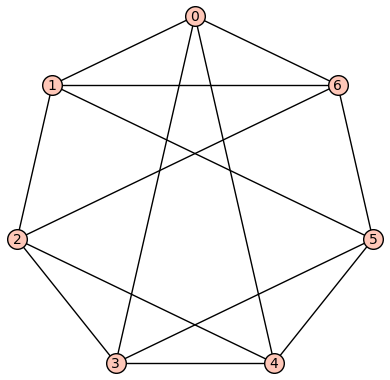
\includegraphics[height=5cm,width=5cm]{graphics/graph_d4reg7b.png}
\end{center}
\begin{center}
%\vspace{8.0 cm}
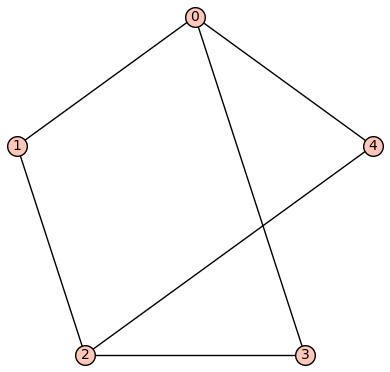
\includegraphics[height=4cm,width=4cm]{graphics/K23-quotient-of-d4reg7b.png}
\end{center}
\end{minipage}
\caption{The quartic graph $\Gamma_2$ ({\tt d4reg7b}), with a degree two harmonic quotient morphism to the $K_{2,3}$ graph, $\Gamma_1=\Gamma_2/G$.}
\label{fig:harmonic-quotient_d7reg7b+K23}
\end{figure}

Two of the remaining $26$ are distinct harmonic quotient morphisms
$\pi: \Gamma_2\to \Gamma_1=\Gamma_2/G$,
for some $G$, where $\Gamma_1$ is the graph \verb+DF{+,
a $5$-graph\footnote{This is the graph6 notation. In the ISGCI notation, it is $\overline{K_3\cup 2K_1}$.}.
An example for
\[
G = \langle (1,3)(4,6) \rangle,
\]
which is in fact a homomorphism,
is tabulated below and the uncolored graphs are depicted in
Figure \ref{fig:harmonic-quotient_d4reg7b+fan5}.


\begin{center}
\begin{tabular}{c|c|c|c}  
  $x$ & $\phi(x)$ & $m_\phi(x)$ & $\nu_\phi(x)$ \\ \hline
  0   &    4   &        2         &  0   \\ 
  1   &    3   &        1         &  0  \\ 
  2   &    0   &        2         &  0  \\ 
  3   &    3   &        1         &  0  \\ 
  4   &    1   &        1         &  0   \\
  5   &    2   &        2         &  0   \\
  6   &    1   &        1         &  0   \\   
\end{tabular}
\end{center}

\[
  \genus(\Gamma_2) =8,\ \ \ \ \
  \genus(\Gamma_1) =3,
\]

\[
\deg(\phi) =2.
\]

\begin{figure}[H]
\begin{minipage}{\textwidth}
\begin{center}
%\vspace{8.0 cm}
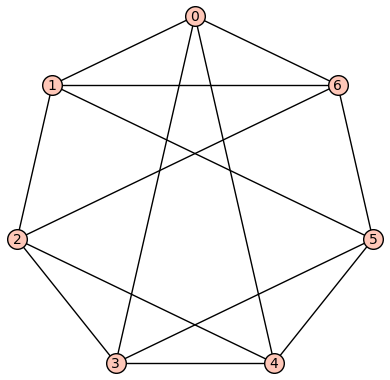
\includegraphics[height=5cm,width=5cm]{graphics/graph_d4reg7b.png}
\end{center}
\begin{center}
%\vspace{8.0 cm}
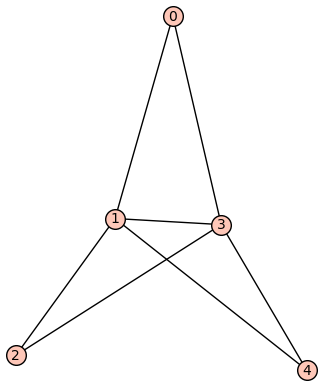
\includegraphics[height=4cm,width=4cm]{graphics/fan5-quotient-of-d4reg7b.png}
\end{center}
\end{minipage}
\cprotect\caption{The quartic graph  $\Gamma_2$ ({\tt d4reg7b}), with a degree two harmonic quotient morphism to the the graph $\Gamma_1=\Gamma_2/G$.}
\label{fig:harmonic-quotient_d4reg7b+fan5}
\end{figure}

Three of the remaining $24$ are (not necessarily distinct)
harmonic quotient morphisms
$\pi: \Gamma_2\to \Gamma_1=\Gamma_2/G$,
for some $G$, where $\Gamma_1=St_4$ is the star graph.
\index{star graph}

Eight of the remaining $21$ are (not necessarily distinct)
harmonic quotient morphisms
$\pi: \Gamma_2\to \Gamma_1=\Gamma_2/G$,
for some $G$, where $\Gamma_1=P_3$ is the path graph on $3$ vertices (all eight give the same morphism).

The remaining $13$ (one of them for $G=\Aut(\Gamma_2)$, all giving the same morphism) are
harmonic quotient morphisms
$\pi: \Gamma_2\to \Gamma_1=\Gamma_2/G$,
for some $G$, where $\Gamma_1=P_2$ is the path graph on $2$ vertices.

}
\end{example}
  

  
\subsection{\texorpdfstring{$8$}{8} vertices}
\label{sec:d4reg8}

This subsection describes the connected quartic graphs on $8$ vertices.
It records their invariants and harmonic morphism counts, and then
works out harmonic quotient morphisms in examples.


There are (up to isomorphism) exactly six $4$-regular connected
graphs on $8$ vertices, $V=\{0,1,2,3,4,5,6,7\}$.
By Ore's Theorem, all of these graphs are Hamiltonian.

\begin{enumerate}
\item
{\tt d4reg8a}
\newline
Define the graph $\Gamma = (V,E)$, where


\[
E = \{
(0, 1), (0, 5), (0, 6), (0, 7), (1, 3), (1, 6), (1, 7), (2, 3), (2, 4),
\]
\[
(2, 5), (2, 7), (3, 4), (3, 6), (4, 5), (4, 6), (5, 7)
\}.
\]
It has diameter $2$,
girth $3$, circumference $8$,
chromatic number $4$, 
and automorphism group of size $16$.
This graph is vertex transitive but not edge transitive.
%aut gp size:  16 
%aut gp gens:  [(1,7)(2,3)(5,6), (0,1)(2,4)(3,5)(6,7)]
The size of the critical group of this graph is $3528=2^3 3^2 7^2$.
\index{vertex transitive graph}

There are no non-trivial harmonic morphisms from $\Gamma$ to
$St_4$, $P_3$, $P_4$, $C_4$, or to $K_4$. However, there are $12$
non-trivial harmonic morphisms from $\Gamma$ to $C_3$.

\item
{\tt d4reg8b}
\newline  
Define the graph $\Gamma = (V,E)$, where

\[
E =
\{
(0, 1), (0, 2), (0, 3), (0, 6), (1, 2), (1, 3), (1, 4), (2, 3),
\]
\[
(2, 7), (3, 5), (4, 5), (4, 6), (4, 7), (5, 6), (5, 7), (6, 7)
\}.
\]
It has diameter $2$, girth $3$, circumference $8$,
chromatic number $4$, and automorphism group of size $48$.
This graph is vertex transitive but not edge transitive.
%aut gp size:  48
%aut gp gens:  [(2,3)(5,7), (1,3)(4,5), (0,1,3)(4,5,6), (0,4)(1,6)(2,5)(3,7)] 
The size of the critical group of this graph is $3456=2^7 3^3$.
\index{vertex transitive graph}

There are $24$ non-trivial harmonic morphisms from $\Gamma$ to $K_4$,
$36$ non-trivial harmonic morphisms from $\Gamma$ to $C_3$,
but no non-trivial harmonic morphisms to $St_4$, $P_3$, $P_4$, or to $C_4$.

\item
{\tt d4reg8c}
\newline  
Define the graph $\Gamma = (V,E)$, where

\[
E = \{
(0, 1), (0, 2), (0, 5), (0, 6), (1, 3), (1, 4), (1, 7), (2, 3),
\]
\[
(2, 4), (2, 7), (3, 5), (3, 6), (4, 5), (4, 6), (5, 7), (6, 7)
\}.
\]
This graph is isomorphic to the complete bipartite graph
$K_{4,4}$.
\index{complete bipartite graph}
It has diameter $2$,
girth $4$, circumference $8$,
chromatic number $2$, 
critical group of size $4096 = 2^{12}$, 
and automorphism group of size $1152$.
It is also a circulant graph with parameters
$(8, [1, 3, 5, 7])$.
\index{circulant graph}
This graph is both vertex transitive and edge transitive,
and is strongly regular with ``trivial'' paramemters $(8,4,0,4)$.
%aut gp size:  1152
%aut gp gens:  [(5,6), (4,7), (3,4), (2,5), (1,2), (0,1)(2,3)(4,5)(6,7)] 
\index{vertex transitive graph}
\index{edge transitive graph}

There are $36$ non-trivial harmonic morphisms from $\Gamma$ to $P_3$,
$72$ non-trivial harmonic morphisms\footnote{Moreover, it appears that
  all of these are multicovers.} from $\Gamma$ to $C_4$,
$576$ non-trivial harmonic
morphisms\footnote{Moreover, it appears that all of these
  are quasicovers.}
from $\Gamma$ to $K_4$, and
$48$ non-trivial harmonic morphisms from $\Gamma$ to $St_4$.
However, it has
no non-trivial harmonic morphisms from $\Gamma$ to $C_3$ or to $P_4$.

\item
{\tt d4reg8d}
\newline  
Define the graph $\Gamma = (V,E)$, where

\[
E = \{
(0, 1), (0, 2), (0, 4), (0, 6), (1, 3), (1, 5), (1, 6), (2, 3),
\]
\[
(2, 5), (2, 7), (3, 4), (3, 7), (4, 5), (4, 6), (5, 7), (6, 7)
\}.
\]
It has diameter $2$,
girth $3$, circumference $8$,
chromatic number $3$, 
critical group of size $3840 = 2^8 3 \cdot 5$, 
and automorphism group of size $16$.
This graph is neither vertex transitive nor edge transitive.
%aut gp size:  16
%aut gp gens:  [(3,5), (1,4), (0,2)(1,3)(4,5)(6,7), (0,6)(2,7)] 

There are no non-trivial harmonic morphisms from $\Gamma$ to $St_4$,
$P_4$ or to $C_4$. However,
there are $4$ non-trivial harmonic morphisms to $P_3$,
$6$ non-trivial harmonic morphisms to $C_3$,
and $48$ non-trivial harmonic morphisms\footnote{Moreover,
  it appears that all of these are quasicovers.}
to $K_4$.

\item
{\tt d4reg8e}
\newline  
Define the graph $\Gamma = (V,E)$, where

\[
E = \{
(0, 1), (0, 2), (0, 6), (0, 7), (1, 3), (1, 4), (1, 5), (2, 3), 
\]
\[
(2, 4), (2, 7), (3, 5), (3, 7), (4, 5), (4, 6), (5, 6), (6, 7)
\}.
\]
It has diameter $2$,
girth $3$, circumference $8$,
chromatic number $3$, 
critical group of size $3696 = 2^4 3\cdot 7\cdot 11$, 
and automorphism group of size $4$.
%aut gp size:  4 
%aut gp gens:  [(0,1)(2,4)(3,6)(5,7), (0,2)(1,4)(3,6)]

There are no non-trivial harmonic morphisms from $\Gamma$ to $St_4$,
$P_3$, $P_4$, $C_4$ or to $K_4$, but there are $6$ non-trivial harmonic
morphisms to $C_3$.

\item
{\tt d4reg8f}
\newline  
Define the graph $\Gamma = (V,E)$, where

\[
E = \{
(0, 1), (0, 2), (0, 6), (0, 7), (1, 2), (1, 3), (1, 4), (2, 3),
\]
\[
(2, 4), (3, 5), (3, 7), (4, 5), (4, 6), (5, 6), (5, 7), (6, 7)
\}.
\]
It has diameter $2$,
girth $3$, circumference $8$,
chromatic number $4$, 
critical group of size $3610 = 2\cdot 5\cdot 19^2$, 
and automorphism group of size $12$.
%aut gp size:  4 
%aut gp gens:  [(0,1)(2,4)(3,6)(5,7), (0,2)(1,4)(3,6)]

There are no non-trivial harmonic morphisms from $\Gamma$ to $St_4$, $P_4$, $C_3$, $C_4$ or to $K_4$. However, there are $2$ non-trivial harmonic
morphisms to $P_3$.

\end{enumerate}



\subsubsection{Examples}

Each example below takes one graph from the list above and describes
its harmonic quotient morphisms.


\begin{example}% d4reg8a
\label{example:d4reg8a}
 {\tt d4reg8a}\newline
{\rm  
  Let $\Gamma_2$ denote the graph {\tt d4reg8a} as given above.
There are $10$ (not necessarily distinct) harmonic quotient morphisms
$\pi: \Gamma_2\to \Gamma_1=\Gamma_2/G$,
for some $G$.

Four of these $10$ are distinct harmonic quotient morphisms
$\pi: \Gamma_2\to \Gamma_1=\Gamma_2/G$,
for some $G$, where $\Gamma_1$ is the \verb+Dh{+ graph\footnote{This is the graph6 notation. In the ISGCI notation, it is called a gem graph or a $3$-fan.}.
\index{gem graph}
An example for
\[
G = \langle  (1,7)(2,3)(5,6)\rangle,
\]
is tabulated below and the uncolored graphs are depicted in
Figure \ref{fig:harmonic-quotient_d4reg8a+gem}.

\begin{center}
\begin{tabular}{c|c|c|c}  
  $x$ & $\phi(x)$ & $m_\phi(x)$ & $\nu_\phi(x)$ \\ \hline
  0   &    4   &        2         &  0   \\ 
  1   &    1   &        1         &  1  \\ 
  2   &    2   &        1         &  1  \\ 
  3   &    2   &        1         &  1  \\ 
  4   &    3   &        2         &  0   \\
  5   &    0   &        1         &  0   \\
  6   &    0   &        1         &  0   \\
  7   &    1   &        1         &  1   \\     
\end{tabular}
\end{center}

\[
  \genus(\Gamma_2) =9,\ \ \ \ \
  \genus(\Gamma_1) =3,
\]

\[
\deg(\phi) =2.
\]

\begin{figure}[H]
\begin{minipage}{\textwidth}
\begin{center}
%\vspace{8.0 cm}
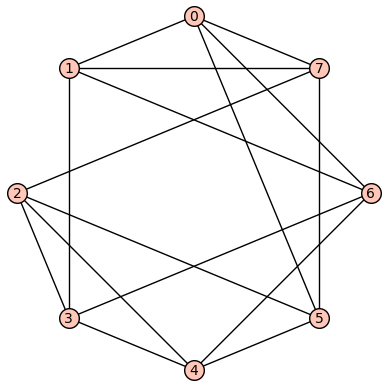
\includegraphics[height=5cm,width=5cm]{graphics/graph_d4reg8a.png}
\end{center}
\begin{center}
%\vspace{8.0 cm}
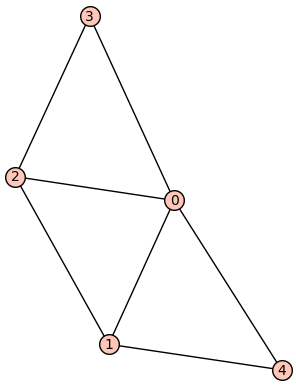
\includegraphics[height=4cm,width=4cm]{graphics/gem-quotient-of-d4reg8a.png}
\end{center}
\end{minipage}
\cprotect\caption{The quartic graph  $\Gamma_2$ ({\tt d4reg8a}), with a degree two harmonic quotient morphism to the graph $\Gamma_1=\Gamma_2/G$.}
\label{fig:harmonic-quotient_d4reg8a+gem}
\end{figure}

Two of the remaining $6$ are distinct harmonic quotient morphisms
$\pi: \Gamma_2\to \Gamma_1=\Gamma_2/G$,
for some $G$, where $\Gamma_1=C_3$. The rest are (not necessarily distinct) 
harmonic quotient morphisms
$\pi: \Gamma_2\to \Gamma_1=\Gamma_2/G$,
for some $G$, where $\Gamma_1=P_2$.

}
\end{example}




\begin{example}% d4reg8b
\label{example:d4reg8b}
 {\tt d4reg8b}\newline
{\rm  
  Let $\Gamma_2$ denote the graph {\tt d4reg8b} as given above.
There are $46$ (not necessarily distinct) harmonic quotient morphisms
$\pi: \Gamma_2\to \Gamma_1=\Gamma_2/G$,
for some $G$.

Exactly one of these $46$ is a distinct harmonic quotient morphism
$\pi: \Gamma_2\to \Gamma_1=\Gamma_2/G$,
for some $G$, where $\Gamma_1=K_4$. In fact, it is a quasicover.
This example, for

\[
G = \langle (0,6)(1,4)(2,7)(3,5)  \rangle,
\]
is tabulated below and depicted in Figure \ref{fig:harmonic-quotient_d4reg8b+K4}.

\begin{center}
\begin{tabular}{c|c|c|c}  
  $x$ & $\phi(x)$ & $m_\phi(x)$ & $\nu_\phi(x)$ \\ \hline
  0   &    2   &        1         &  1   \\ 
  1   &    0   &        1         &  1  \\ 
  2   &    1   &        1         &  1  \\ 
  3   &    3   &        1         &  1  \\ 
  4   &    0   &        1         &  1   \\
  5   &    3   &        1         &  1   \\
  6   &    2   &        1         &  1   \\
  7   &    1   &        1         &  1   \\     
\end{tabular}
\end{center}

\[
  \genus(\Gamma_2) =9,\ \ \ \ \
  \genus(\Gamma_1) =3,
\]

\[
\deg(\phi) =2.
\]
\begin{figure}[H]
\begin{minipage}{\textwidth}
\begin{center}
%\vspace{8.0 cm}
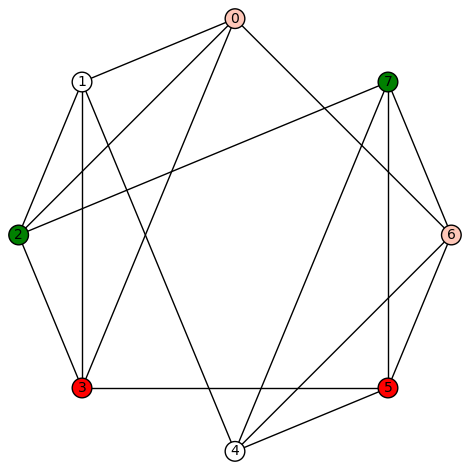
\includegraphics[height=5cm,width=5cm]{graphics/harmonic-quotient_d4reg8b-K4_20130321.png}
\end{center}
\begin{center}
%\vspace{8.0 cm}
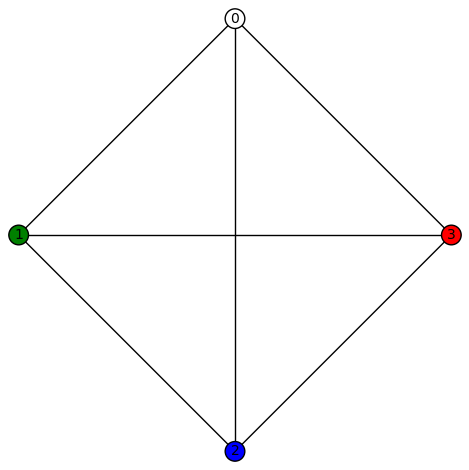
\includegraphics[height=4cm,width=4cm]{graphics/K4-quotient-of-d4reg8b_0123.png}
\end{center}
\end{minipage}
\caption{The quartic graph  $\Gamma_2$, with a degree two harmonic quotient morphism to the complete graph, $\Gamma_1=K_4$.}
\label{fig:harmonic-quotient_d4reg8b+K4}
\end{figure}


Six of the remaining $45$ are distinct harmonic quotient morphisms
$\pi: \Gamma_2\to \Gamma_1=\Gamma_2/G$,
for some $G$, where $\Gamma_1=C_3$.

The remaining $39$ are (not necessarily distinct)
harmonic quotient morphisms
$\pi: \Gamma_2\to \Gamma_1=\Gamma_2/G$,
for some $G$, where $\Gamma_1=P_2$.

}
\end{example}




\begin{example}% d4reg8c
\label{example:d4reg8c}
 {\tt d4reg8c}\newline
{\rm  
  Let $\Gamma_2$ denote the graph $K_{4,4}$ as given above.
There are $2221$ (not necessarily distinct) harmonic quotient morphisms
$\pi: \Gamma_2\to \Gamma_1=\Gamma_2/G$,
for some $G$.

Of these $2221$, $24$ are (not necessarily distinct) harmonic quotient morphisms
$\pi: \Gamma_2\to \Gamma_2/G = K_4$, for some $G$. In fact, each of the $24$ is a quasicover.
Of the remaining $2191$, $234$ are (not necessarily distinct) harmonic quotient morphisms
$\pi: \Gamma_2\to \Gamma_2/G = C_4$, for some $G$.
Of the remaining $1963$, $636$ are (not necessarily distinct) harmonic quotient morphisms
$\pi: \Gamma_2\to \Gamma_2/G = P_3$, for some $G$.
The remaining $1327$ consist of $12$ quotients with $6$ vertices,
$18$ quotients to the star graph $St_5$, and $1297$ quotients to $P_2$.
}
\end{example}




\begin{example}% d4reg8d
\label{example:d4reg8d}
 {\tt d4reg8d}\newline
{\rm  
  Let $\Gamma_2$ denote the graph {\tt d4reg8d} as given above.
There are $12$ (not necessarily distinct) harmonic quotient morphisms
$\pi: \Gamma_2\to \Gamma_1=\Gamma_2/G$,
for some $G$.

Of these $11$, $2$ are distinct harmonic quotient morphisms
$\pi: \Gamma_2\to \Gamma_2/G = K_4$, for some $G$. In fact, they are each a quasicover.
Of the remaining $10$, $3$ are (not necessarily distinct) harmonic quotient morphisms
$\pi: \Gamma_2\to \Gamma_2/G = C_3$, for some $G$.
The remaining $7$ (one of them for $G=\Aut(\Gamma_2)$) are (not necessarily distinct) harmonic quotient morphisms
$\pi: \Gamma_2\to \Gamma_2/G = P_2$, for some $G$.
}
\end{example}





\begin{example}% d4reg8e
\label{example:d4reg8e}
 {\tt d4reg8e}\newline
{\rm  
  Let $\Gamma_2$ denote the graph {\tt d4reg8e} as given above.
There are exactly two harmonic quotient morphisms
$\pi: \Gamma_2\to \Gamma_1=\Gamma_2/G$,
for some subgroup $G$ of $\Aut(\Gamma_2)$.
For $G=\Aut(\Gamma_2)$ (of order $4$) the quotient is $C_3$, with fibers
$\{0,1,2,4\}$, $\{3,6\}$, $\{5,7\}$.
The other, tabulated below, is a quotient morphism
$\phi: \Gamma_2\to \Gamma_1=\Gamma_2/G$,
where $\Gamma_1$ is the gem graph and

\[
G = \langle (0,2)(1,4)(3,6) \rangle,
\]
is tabulated below.

\begin{center}
\begin{tabular}{c|c|c|c}  
  $x$ & $\phi(x)$ & $m_\phi(x)$ & $\nu_\phi(x)$ \\ \hline
  0   &    2   &        1         &  1   \\ 
  1   &    0   &        1         &  1  \\ 
  2   &    2   &        1         &  1  \\ 
  3   &    3   &        1         &  0  \\ 
  4   &    0   &        1         &  1   \\
  5   &    1   &        2         &  0   \\
  6   &    3   &        1         &  0   \\
  7   &    4   &        2         &  0   \\     
\end{tabular}
\end{center}

\[
  \genus(\Gamma_2) =9,\ \ \ \ \
  \genus(\Gamma_1) =3,
\]

\[
\deg(\phi) =2.
\]

}
\end{example}



\begin{example}% d4reg8f
\label{example:d4reg8f}
 {\tt d4reg8f}\newline
{\rm  
  Let $\Gamma_2$ denote the graph {\tt d4reg8f} as given above.
There are three (identical) harmonic quotient morphisms
$\pi: \Gamma_2\to \Gamma_1=\Gamma_2/G$,
for some subgroup $G$ of $\Aut(\Gamma_2)$.
Each of these is a quotient morphism
$\phi: \Gamma_2\to \Gamma_1=\Gamma_2/G$,
where $\Gamma_1=P_3$ (in each case, the vertices of $P_3$
are labeled in such a way that $0$ has degree $2$).
One such subgroup is

\[
G_1 = \langle (1,2), (0,4,3)(5,7,6) \rangle,
\]
another is

\[
G_2 = \langle (1,2)(3,4)(6,7), (0,4,3)(5,7,6) \rangle,
\]
and the third is $\Aut(\Gamma_2)$, of order $12$.
The first two have cardinality $6$. We tabulate
$\phi_1: \Gamma_2\to \Gamma_1=\Gamma_2/G_1=P_3$
below.

\begin{center}
\begin{tabular}{c|c|c|c}  
  $x$ & $\phi(x)$ & $m_\phi(x)$ & $\nu_\phi(x)$ \\ \hline
  0   &    0   &        2         &  0   \\ 
  1   &    2   &        3         &  1  \\ 
  2   &    2   &        3         &  1  \\ 
  3   &    0   &        2         &  0  \\ 
  4   &    0   &        2         &  0   \\
  5   &    1   &        2         &  2   \\
  6   &    1   &        2         &  2   \\
  7   &    1   &        2         &  2   \\     
\end{tabular}
\end{center}

\[
  \genus(\Gamma_2) =9,\ \ \ \ \
  \genus(\Gamma_1) =0,
\]

\[
\deg(\phi) =6.
\]

}
\end{example}


\subsection{\texorpdfstring{$9$}{9} vertices}
\label{sec:d4reg9}

This subsection describes a selection of the connected quartic graphs on $9$ vertices.
It records their invariants and harmonic morphism counts, and then
works out harmonic quotient morphisms in examples.


There are (up to isomorphism) exactly $16$ $4$-regular connected graphs on $9$ vertices.
%For the majority of these, it's currently unknown how many (if any)
%non-trivial harmonic morphisms map from these graphs to $C_4$ or $K_4$.
Below, we include $9$ of these $16$ as examples.

\begin{enumerate}
\item
  {\tt d4reg9a}\newline
Define the graph  $\Gamma$ to have edge set:

\[
E = \{
(0, 1), (0, 2), (0, 7), (0, 8), (1, 2), (1, 3), (1, 7), (2, 3), (2, 8),
\]
\[
 (3, 4), (3, 5), (4, 5), (4, 6), (4, 8), (5, 6), (5, 7), (6, 7), (6, 8)
\}.
\]
It has diameter $2$,
girth $3$, circumference $9$ (i.e., it's Hamiltonian),
critical group of size $10800 = 2^43^35^2$, 
and automorphism group of size $12$.

There are no non-trivial harmonic morphisms from $\Gamma$ to $St_4$,
$P_4$, $C_4$, or to $K_4$.  However, there are $2$ non-trivial
harmonic morphisms from $\Gamma$ to $P_3$ and $24$ non-trivial
harmonic morphisms from $\Gamma$ to $C_3$.

\item
  {\tt d4reg9b}\newline  
Define the graph $\Gamma$ to have edge set:

\[
E = \{
(0, 1), (0, 3), (0, 7), (0, 8), (1, 2), (1, 3), (1, 7), (2, 3), (2, 5), (2, 8),
\]
\[
(3, 4), (4, 5), (4, 6), (4, 8), (5, 6), (5, 7), (6, 7), (6, 8)
\}.
\]
It has diameter $2$,
girth $3$, circumference $9$ (i.e., it's Hamiltonian),
critical group of size $11360 = 2^5 5\cdot 71$, 
and automorphism group of size $2$.

There are no non-trivial harmonic morphisms from $\Gamma$ to
$St_4$, $P_3$, $P_4$, $C_3$, $C_4$, or to $K_4$.  

\item
{\tt d4reg9c}\newline  
Define the graph $\Gamma$ to have edge set:

\[
E = \{
(0, 1), (0, 2), (0, 7), (0, 8), (1, 2), (1, 3), (1, 4), (2, 3), (2, 8), 
\]
\[
(3, 4), (3, 5), (4, 5), (4, 6), (5, 6), (5, 7), (6, 7), (6, 8), (7, 8)
\}.
\]
It has diameter $2$,
girth $3$, circumference $9$ (i.e., it's Hamiltonian),
critical group of size $10404 = 2^2 3^2 17^2$, 
and automorphism group of size $18$.
This is a vertex transitive but not edge transitive graph.
\index{vertex transitive graph}

There are no non-trivial harmonic morphisms from $\Gamma$ to $St_4$,
$P_3$, $P_4$, $C_4$, or to $K_4$.  However, there
are $6$ non-trivial harmonic morphisms from $\Gamma$ to $C_3$. 

\item
{\tt d4reg9d}\newline
Define the graph $\Gamma$ to have edge set:

\[
E = \{
(0, 1), (0, 5), (0, 7), (0, 8), (1, 2), (1, 4), (1, 7), (2, 3), (2, 4), (2, 5),
\]
\[
(3, 4), (3, 6), (3, 8), (4, 5), (5, 6), (6, 7), (6, 8), (7, 8)
\}.
\]
It has diameter $2$,
girth $3$, circumference $9$ (i.e., it's Hamiltonian),
critical group of size $11005 = 5\cdot 31\cdot 71$, 
and automorphism group of size $4$.

There are no non-trivial harmonic morphisms from $\Gamma$ to
$P_4$, $C_3$, $C_4$, or to $K_4$. However, there are $2$ non-trivial harmonic
morphisms from $\Gamma$ to $P_3$. 


\item
{\tt d4reg9e}\newline  
Define the graph $\Gamma$ to have edge set:

\[
E = \{
(0, 1), (0, 3), (0, 5), (0, 8), (1, 2), (1, 4), (1, 7), (2, 3), (2, 5), (2, 7),
\]
\[
 (3, 4), (3, 8), (4, 5), (4, 6), (5, 6), (6, 7), (6, 8), (7, 8)
\}.
\]
It has diameter $2$,
girth $3$, circumference $9$ (i.e., it's Hamiltonian),
critical group of size $12096 = 2^6 3^3 7$, 
and automorphism group of size $12$.

There are no non-trivial harmonic morphisms from $\Gamma$ to $St_4$,
$P_4$, $C_4$, or to $K_4$. However,
there are $6$ non-trivial harmonic
morphisms\footnote{Moreover,
  it appears that all of these are quasicovers
  (with constant horizontal multiplicity $1$ and constant vertical
  multiplicity $2$).}
from $\Gamma$ to $C_3$,
and $6$ non-trivial harmonic morphisms from $\Gamma$ to $P_3$.


\item
{\tt d4reg9f}\newline    
  Define the graph $\Gamma$
  %d4reg9l=d4reg9-12
  to have edge set:

\[
E = \{
(0, 1), (0, 3), (0, 6), (0, 8), (1, 2), (1, 4), (1, 6), (2, 3), (2, 5), (2, 7), (3, 4),
\]
\[
(3, 7), (4, 5), (4, 8), (5, 6), (5, 8), (6, 7), (7, 8)
\}.
\]
It has diameter $2$,
girth $3$, circumference $9$ (i.e., it's Hamiltonian),
critical group of size $12321 = 3^2 37^2$, 
and automorphism group of size $18$.
This is a vertex transitive but not edge transitive graph.
\index{vertex transitive graph}

There are no non-trivial harmonic morphisms from $\Gamma$ to $St_4$,
$P_3$, $P_4$, $C_4$, or to $K_4$. However,
there are $6$ non-trivial harmonic morphisms from $\Gamma$ to $C_3$.

\item
{\tt d4reg9g}\newline    
  Define the graph $\Gamma$
  %d4reg9n=d4reg9-14
  to have edge set:

\[
E = \{
(0, 1), (0, 3), (0, 4), (0, 8), (1, 2), (1, 5), (1, 8), (2, 3), (2, 5), (2, 7), (3, 4),
\]
\[
 (3, 7), (4, 5), (4, 6), (5, 6), (6, 7), (6, 8), (7, 8)
\}.
\]
It has diameter $2$,
girth $3$, circumference $9$ (i.e., it's Hamiltonian),
critical group of size $11664 = 2^4 3^6$, 
and automorphism group of size $72$.
This is a vertex transitive, edge transitive, arc transitive,
and distance regular graph.
Morover, it's $(9,4,1,2)$-strongly regular, isomorphic to the Paley graph
on $9$ vertices.
\index{vertex transitive graph}
\index{edge transitive graph}
\index{arc transitive graph}
\index{distance regular graph}
\index{strongly regular graph}
\index{Paley graph}

There are no non-trivial harmonic morphisms from $\Gamma$ to $St_4$,
$P_4$, $C_4$. or to $K_4$. However, there are $18$ non-trivial
harmonic morphisms from $\Gamma$ to $P_3$
and $78$ non-trivial harmonic
morphisms\footnote{Moreover,
  some, not not all, of these are quasicovers
  (with constant horizontal multiplicity $1$ and constant vertical
  multiplicity $2$).} from $\Gamma$ to $C_3$.
\label{page:paley9}

\item
{\tt d4reg9h}\newline    
\label{page:d4reg9-15}  
  Define the graph $\Gamma$ 
% d4reg9-15 ## integral spectrum [4, 2, 1, 0, 0, -1, -1, -2, -3]
  % ## denoted I_{9,3} in [CSS98]
to have edge set:

\[
E = \{
(0, 1), (0, 4), (0, 6), (0, 8), (1, 2), (1, 3), (1, 5), (2, 3),
\]
\[
(2, 4), (2, 7), (3, 4), (3, 7), (4, 5), (5, 6), (5, 8), (6, 7), (6, 8), (7, 8)
\}.
\]
It is an integral graph with diameter $2$,
girth $3$, circumference $9$ (i.e., it's Hamiltonian),
critical group of size $11200 = 2^6 5^27$, 
and automorphism group of size $32$.
It has no non-trivial harmonic morphisms to 
$C_3$, $C_4$, $P_4$, $K_4$, but $8$ non-trivial harmonic morphisms to
$P_3$.

See also page \pageref{page:d4reg9-15} below.
  
\item
{\tt d4reg9i}\newline  
  Define the graph $\Gamma$
  % d4reg9p
  to have edge set:

\[
E = \{
(0, 1), (0, 3), (0, 7), (0, 8), (1, 2), (1, 4), (1, 5), (2, 3), (2, 4), (2, 5),
\]
\[
(3, 7), (3, 8), (4, 5), (4, 6), (5, 6), (6, 7), (6, 8), (7, 8)
\}.
\]
It has diameter $2$,
girth $3$, circumference $9$ (i.e., it's Hamiltonian),
critical group of size $9600 = 2^7 3 \cdot 5^2$, 
and automorphism group of size $16$.

There are no non-trivial harmonic morphisms from $\Gamma$ to $St_4$,
$P_3$, $P_4$, $C_4$, or to $K_4$. However, there are
exactly $6$ non-trivial harmonic morphisms from $\Gamma$ to $C_3$.


\end{enumerate}

\subsubsection{Examples}

Each example below takes one graph from the list above and describes
its harmonic quotient morphisms.



\begin{example}% d4reg9a
\label{example:d4reg9a}
 {\tt d4reg9a}\newline
{\rm  
  Let $\Gamma_2$ denote the graph {\tt d4reg9a} as given above.
There are $12$ harmonic quotient morphisms
$\pi: \Gamma_2\to \Gamma_1=\Gamma_2/G$,
for some subgroup $G$ of $\Aut(\Gamma_2)$.

Three of these harmonic quotient morphisms are to the co-antenna graph.
For example, if 
\index{coantenna graph}

\[
G = \langle (1,2)(4,5)(7,8) \rangle.
\]
We tabulate $\phi_1: \Gamma_2\to \Gamma_1=\Gamma_2/G$
below and give the uncolored graphs in Figure \ref{fig:harmonic-quotient_d4reg9a+coantenna}.

\begin{center}
\begin{tabular}{c|c|c|c}  
  $x$ & $\phi(x)$ & $m_\phi(x)$ & $\nu_\phi(x)$ \\ \hline
  0   &    1   &        2         &  0   \\
  1   &    3   &        1         &  1   \\
  2   &    3   &        1         &  1   \\
  3   &    0   &        2         &  0   \\
  4   &    2   &        1         &  1   \\
  5   &    2   &        1         &  1   \\
  6   &    4   &        2         &  0   \\
  7   &    5   &        1         &  0   \\
  8   &    5   &        1         &  0   \\
\end{tabular}
\end{center}

\[
  \genus(\Gamma_2) =10,\ \ \ \ \
  \genus(\Gamma_1) =3,
\]

\[
\deg(\phi) =2.
\]

\begin{figure}[H]
\begin{minipage}{\textwidth}
\begin{center}
%\vspace{8.0 cm}
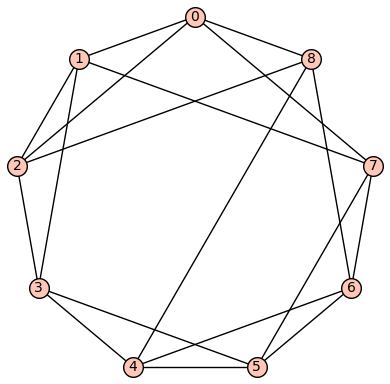
\includegraphics[height=5cm,width=5cm]{graphics/graph_d4reg9a.png}
\end{center}
\begin{center}
%\vspace{8.0 cm}
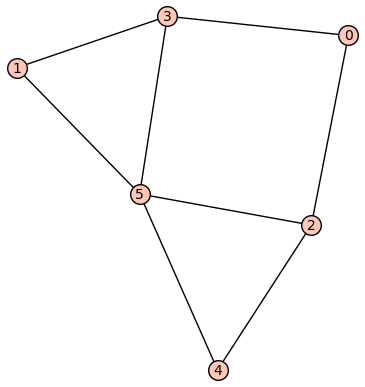
\includegraphics[height=4cm,width=4cm]{graphics/coantenna-quotient-of-d4reg9a.png}
\end{center}
\end{minipage}
\caption{The quartic graph  $\Gamma_2$ ({\tt d4reg9a}), with a degree two harmonic quotient morphism to the coantenna graph, $\Gamma_1$.}
\label{fig:harmonic-quotient_d4reg9a+coantenna}
\end{figure}


One of the remaining $9$ is a harmonic quotient homomorphism
$\phi: \Gamma_2\to \Gamma_1=\Gamma_2/G$,
where $\Gamma_1=S_3$, where
\index{$S_3$ graph}

\[
G = \langle (0,6)(1,5)(2,4) \rangle.
\]
We tabulate $\phi_1: \Gamma_2\to \Gamma_1=\Gamma_2/G=S_3$
below and give the uncolored graphs in Figure \ref{fig:harmonic-quotient_d4reg9a+S3}.

\begin{center}
\begin{tabular}{c|c|c|c}  
  $x$ & $\phi(x)$ & $m_\phi(x)$ & $\nu_\phi(x)$ \\ \hline
  0   &    3   &        1         &  0   \\
  1   &    2   &        1         &  0   \\
  2   &    1   &        1         &  0   \\
  3   &    0   &        2         &  0   \\
  4   &    1   &        1         &  0   \\
  5   &    2   &        1         &  0   \\
  6   &    3   &        1         &  0   \\
  7   &    5   &        2         &  0   \\
  8   &    4   &        2         &  0   \\
\end{tabular}
\end{center}

\[
  \genus(\Gamma_2) =10,\ \ \ \ \
  \genus(\Gamma_1) =4,
\]

\[
\deg(\phi) =2.
\]

\begin{figure}[H]
\begin{minipage}{\textwidth}
\begin{center}
%\vspace{8.0 cm}
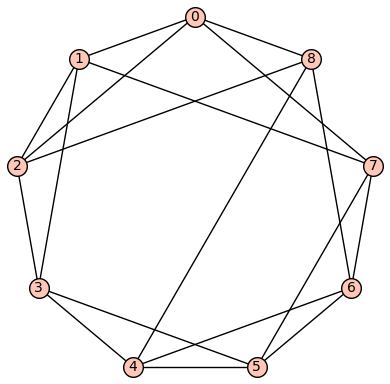
\includegraphics[height=5cm,width=5cm]{graphics/graph_d4reg9a.png}
\end{center}
\begin{center}
%\vspace{8.0 cm}
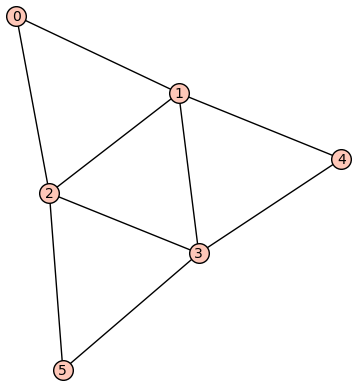
\includegraphics[height=4cm,width=4cm]{graphics/S3-quotient-of-d4reg9a.png}
\end{center}
\end{minipage}
\caption{The quartic graph  $\Gamma_2$ ({\tt d4reg9a}), with a degree two harmonic quotient morphism to the matchstick graph, $\Gamma_1=S_3$.}
\label{fig:harmonic-quotient_d4reg9a+S3}
\end{figure}

All the $8$ remaining harmonic quotients (one of them for $G=\Aut(\Gamma_2)$) map to $P_2$ or $P_3$ or the
paw graph (which is $C_3$ plus a leaf ``tail').
\index{paw graph}
One of these, a harmonic quotient morphisms
$\phi: \Gamma_2\to \Gamma_1=\Gamma_2/G$,
where $\Gamma_1$ is the paw graph and where

\[
G = \langle (1,2)(4,5)(7,8), (0,6)(1,4)(2,5)(7,8) \rangle,
\]
is tabulated below.

\begin{center}
\begin{tabular}{c|c|c|c}  
  $x$ & $\phi(x)$ & $m_\phi(x)$ & $\nu_\phi(x)$ \\ \hline
  0   &    1   &        2         &  0   \\
  1   &    2   &        1         &  1   \\
  2   &    2   &        1         &  1   \\
  3   &    0   &        4         &  0   \\
  4   &    2   &        1         &  1   \\
  5   &    2   &        1         &  1   \\
  6   &    1   &        2         &  0   \\
  7   &    3   &        2         &  0   \\
  8   &    3   &        2         &  0   \\
\end{tabular}
\end{center}

\[
  \genus(\Gamma_2) =10,\ \ \ \ \
  \genus(\Gamma_1) =1,
\]

\[
\deg(\phi) =4.
\]


}
\end{example}


\begin{example}% d4reg9b
\label{example:d4reg9b}
 {\tt d4reg9b}\newline
{\rm  
  Let $\Gamma_2$ denote the graph {\tt d4reg9b} as given above.
There is exactly one harmonic quotient morphism
$\pi: \Gamma_2\to \Gamma_1=\Gamma_2/G$, namely for
$G=\Aut(\Gamma_2)=\langle (0,5)(1,6)(2,8)(3,4)\rangle$. The quotient
has $5$ vertices and $8$ edges.

}
\end{example}


\begin{example}% d4reg9c
\label{example:d4reg9c}
 {\tt d4reg9c}\newline
{\rm  
Let $\Gamma_2$ denote the graph {\tt d4reg9c} as given above.
There are $4$ harmonic quotient morphisms
$\pi: \Gamma_2\to \Gamma_1=\Gamma_2/G$,
for some subgroup $G$ of $\Aut(\Gamma_2)$.

There is only one harmonic quotient morphisms
$\pi: \Gamma_2\to \Gamma_1=\Gamma_2/G$,
for some subgroup $G$ of $\Aut(\Gamma_2)$, to
$\Gamma_1=C_3$. In fact, this is a multicover
of degree $6$ and multiplicity $2$.
In this case,

\[
G = \langle (0,3,6)(1,5,8)(2,4,7) \rangle.
\]
We tabulate $\phi_1: \Gamma_2\to \Gamma_1=\Gamma_2/G=C_3$
below and depict it in Figure \ref{fig:harmonic-quotient_d4reg9c-C3_021012012}.
%harmonic-quotient_d4reg9c-C3_021012012

\begin{center}
\begin{tabular}{c|c|c|c}  
  $x$ & $\phi(x)$ & $m_\phi(x)$ & $\nu_\phi(x)$ \\ \hline
  0   &    0   &        2         &  0   \\ 
  1   &    2   &        2         &  0  \\ 
  2   &    1   &        2         &  0  \\ 
  3   &    0   &        2         &  0  \\ 
  4   &    1   &        2         &  0   \\
  5   &    2   &        2         &  0   \\
  6   &    0   &        2         &  0   \\
  7   &    1   &        2         &  0   \\
  8   &    2   &        2         &  0   \\ 
\end{tabular}
\end{center}

\[
  \genus(\Gamma_2) =10,\ \ \ \ \
  \genus(\Gamma_1) =1,
\]

\[
\deg(\phi) =6.
\]

\begin{figure}[H]
\begin{minipage}{\textwidth}
\begin{center}
%\vspace{8.0 cm}
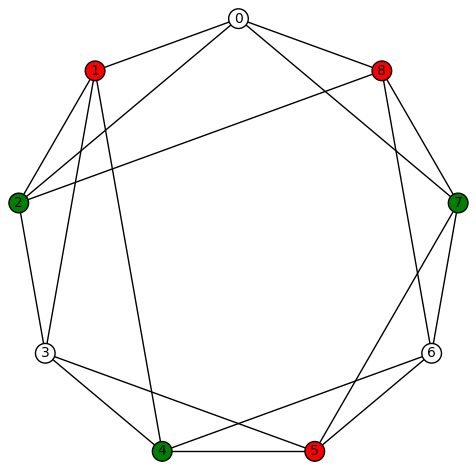
\includegraphics[height=5cm,width=5cm]{graphics/harmonic-quotient_d4reg9c-C3_021012012.png}
\end{center}
\begin{center}
%\vspace{8.0 cm}
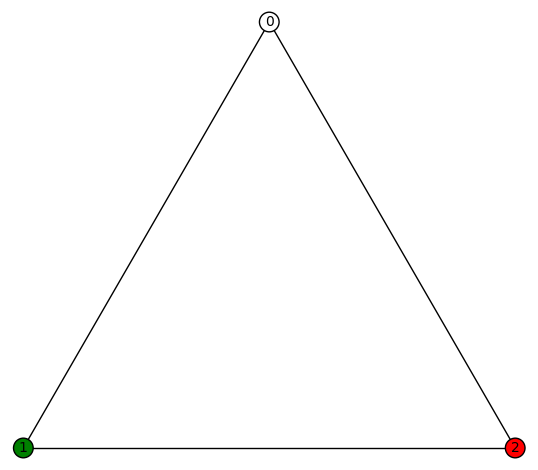
\includegraphics[height=4cm,width=4cm]{graphics/cycle3-012.png}
\end{center}
\end{minipage}
\caption{The quartic graph  $\Gamma_2$ ({\tt d4reg9c}), with a degree six harmonic quotient homomorphism (in fact, a multicover) to the cycle graph, $\Gamma_1=C_3$.}
\label{fig:harmonic-quotient_d4reg9c-C3_021012012}
\end{figure}


}
\end{example}



\begin{example}% d4reg9d
\label{example:d4reg9d}
 {\tt d4reg9d}\newline
{\rm  
  Let $\Gamma_2$ denote the graph {\tt d4reg9d} as given above.
There are no harmonic quotient morphisms
$\pi: \Gamma_2\to \Gamma_1=\Gamma_2/G$,
for some subgroup $G$ of $\Aut(\Gamma_2)$.

}
\end{example}




\begin{example}% d4reg9e
\label{example:d4reg9e}
 {\tt d4reg9e}\newline
{\rm  
Let $\Gamma_2$ denote the graph {\tt d4reg9e} as given above.
There are $6$ harmonic quotient morphisms
$\pi: \Gamma_2\to \Gamma_1=\Gamma_2/G$,
for some subgroup $G$ of $\Aut(\Gamma_2)$.
Three of these $6$ are quotients to the \verb+D]w+
graph\footnote{This is the graph6 notation. However, the ISGCI notation is
$\overline{P_2\cup P_3}$.}. The remaining three are
(identical morphisms but with different subgroups, one of which is $\Aut(\Gamma_2)$)
harmonic quotients to $P_2$.

One of the three distinct harmonic quotient morphisms
$\pi: \Gamma_2\to \Gamma_1=\Gamma_2/G=\Gamma_1=C_4+2C_3$,
for the subgroup

\[
G = \langle (0,1)(2,3)(4,5)(7,8) \rangle.
\]
of $\Aut(\Gamma_2)$, is tabulated below.
In addition, the uncolored graphs are depicted
in Figure \ref{fig:harmonic-quotient_d4reg9e-C4+2C3}.

\begin{center}
\begin{tabular}{c|c|c|c}  
  $x$ & $\phi(x)$ & $m_\phi(x)$ & $\nu_\phi(x)$ \\ \hline
  0   &    3   &        1         &  1   \\ 
  1   &    3   &        1         &  1  \\ 
  2   &    1   &        1         &  1  \\ 
  3   &    1   &        1         &  1  \\ 
  4   &    2   &        1         &  1   \\
  5   &    2   &        1         &  1   \\
  6   &    0   &        2         &  0   \\
  7   &    4   &        1         &  1   \\
  8   &    4   &        1         &  1   \\ 
\end{tabular}
\end{center}

\[
  \genus(\Gamma_2) =10,\ \ \ \ \
  \genus(\Gamma_1) =3,
\]

\[
\deg(\phi) =2.
\]

\begin{figure}[H]
\begin{minipage}{\textwidth}
\begin{center}
%\vspace{8.0 cm}
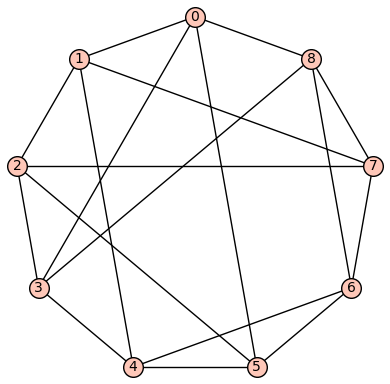
\includegraphics[height=5cm,width=5cm]{graphics/graph_d4reg9e.png}
\end{center}
\begin{center}
%\vspace{8.0 cm}
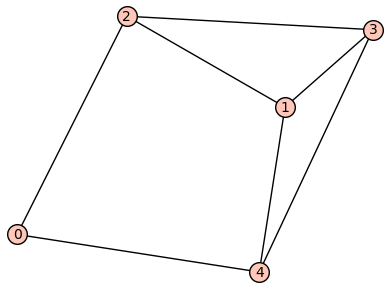
\includegraphics[height=4cm,width=4cm]{graphics/C4+2C3-quotient-of-d4reg9e.png}
\end{center}
\end{minipage}
\cprotect\caption{The quartic graph  $\Gamma_2$ ({\tt d4reg9e}), with a degree two harmonic quotient morphism to the graph \verb+D]w=+$\Gamma_1=\overline{P_2\cup P_3}$.}
\label{fig:harmonic-quotient_d4reg9e-C4+2C3}
\end{figure}

}
\end{example}



\begin{example}% d4reg9f
\label{example:d4reg9f}
 {\tt d4reg9f}\newline
{\rm  
  Let $\Gamma_2$ denote the graph {\tt d4reg9f} as given above.
There are $4$ harmonic quotient morphisms
$\pi: \Gamma_2\to \Gamma_1=\Gamma_2/G$,
for some subgroup $G$ of $\Aut(\Gamma_2)$.

Three of these harmonic quotient morphisms are to the path graph,
$\Gamma_1=P_2$.
One of these harmonic quotient morphisms is to the cycle graph,
$\Gamma_1=C_3$.
If 

\[
G = \langle (0,6,1)(2,3,7)(4,8,5) \rangle,
\]
then the quotient $\phi: \Gamma_2\to \Gamma_1=\Gamma_2/G$,
tabulated below, is in fact a quasicover.

\begin{center}
\begin{tabular}{c|c|c|c}  
  $x$ & $\phi(x)$ & $m_\phi(x)$ & $\nu_\phi(x)$ \\ \hline
  0   &    0   &        1         &  2   \\ 
  1   &    0   &        1         &  2  \\ 
  2   &    1   &        1         &  2  \\ 
  3   &    1   &        1         &  2  \\ 
  4   &    2   &        1         &  2   \\
  5   &    2   &        1         &  2   \\
  6   &    0   &        1         &  2   \\
  7   &    1   &        1         &  2   \\
  8   &    2   &        1         &  2   \\ 
\end{tabular}
\end{center}

\[
  \genus(\Gamma_2) =10,\ \ \ \ \
  \genus(\Gamma_1) =1,
\]
and $\deg(\phi)=3$.

}
\end{example}



\begin{example}% d4reg9g
\label{example:d4reg9g}
 {\tt d4reg9g}\newline
{\rm  
  Let $\Gamma_2$ denote the graph {\tt d4reg9g} as given above.
There are $59$ harmonic quotient morphisms
$\pi: \Gamma_2\to \Gamma_1=\Gamma_2/G$,
for some subgroup $G$ of $\Aut(\Gamma_2)$.

Six of these harmonic quotient morphisms are to the matchstick graph,
$\Gamma_1=S_3$.
\index{$S_3$ graph}
For example, if 

\[
G = \langle (1,3)(4,8)(5,7) \rangle,
\]
then the quotient $\phi: \Gamma_2\to \Gamma_1=\Gamma_2/G$,
tabulated below, is in fact a homomorphism to $\Gamma_1=S_3$.

\begin{center}
\begin{tabular}{c|c|c|c}  
  $x$ & $\phi(x)$ & $m_\phi(x)$ & $\nu_\phi(x)$ \\ \hline
  0   &    5   &        2         &  0   \\ 
  1   &    3   &        1         &  0  \\ 
  2   &    0   &        2         &  0  \\ 
  3   &    3   &        1         &  0  \\ 
  4   &    4   &        1         &  0   \\
  5   &    1   &        1         &  0   \\
  6   &    2   &        2         &  0   \\
  7   &    1   &        1         &  0   \\
  8   &    4   &        1         &  0   \\ 
\end{tabular}
\end{center}

\[
  \genus(\Gamma_2) =10,\ \ \ \ \
  \genus(\Gamma_1) =4,
\]
and $\deg(\phi)=2$.

Of the remaining $53$, $9$ are harmonic quotient morphisms to
the paw graph (i.e., $C_3$ plus a leaf edge).
\index{paw graph}
Of the remaining $44$, $8$ are (not necessarily distinct) harmonic
quotient morphisms to the graph $C_3$.
All of the remaining $36$ are (not necessarily distinct) harmonic
quotient morphisms to the graph $P_2$.

}
\end{example}



\begin{example}% d4reg9h
\label{example:d4reg9h}
 {\tt d4reg9h}\newline
{\rm  
Let $\Gamma_2$ denote the graph {\tt d4reg9h} as given above.
There are $4$ harmonic quotient morphisms
$\pi: \Gamma_2\to \Gamma_1=\Gamma_2/G$,
for some subgroup $G$ of $\Aut(\Gamma_2)$.
All of these are quotients to a graph we shall call
the {\it complete house graph}, however the ISGCI notation is
$\overline{P_3\cup 2K_1}$. 
\index{house graph!complete}
\index{complete house graph}
One of the these harmonic quotient morphisms,
$\pi: \Gamma_2\to \Gamma_1=\Gamma_2/G=\Gamma_1$,
for the subgroup

\[
G = \langle (0,1)(2,6)(3,8)(4,5) \rangle,
\]
is tabulated below.
In addition, the uncolored graphs are depicted
in Figure \ref{fig:harmonic-quotient_d4reg9h-K4+C3}.

\begin{center}
\begin{tabular}{c|c|c|c}  
  $x$ & $\phi(x)$ & $m_\phi(x)$ & $\nu_\phi(x)$ \\ \hline
  0   &    3   &        1         &  1   \\ 
  1   &    3   &        1         &  1  \\ 
  2   &    1   &        1         &  0  \\ 
  3   &    0   &        1         &  0  \\ 
  4   &    2   &        1         &  1   \\
  5   &    2   &        1         &  1   \\
  6   &    1   &        1         &  0   \\
  7   &    4   &        2         &  0   \\
  8   &    0   &        1         &  0   \\ 
\end{tabular}
\end{center}

\[
  \genus(\Gamma_2) =10,\ \ \ \ \
  \genus(\Gamma_1) =4,
\]

\[
\deg(\phi) =2.
\]

\begin{figure}[H]
\begin{minipage}{\textwidth}
\begin{center}
%\vspace{8.0 cm}
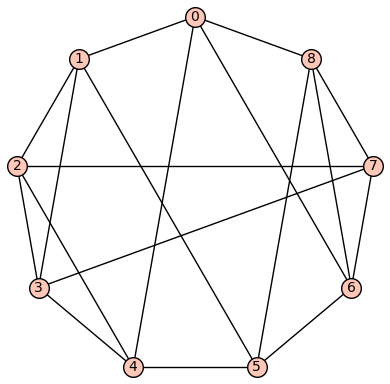
\includegraphics[height=5cm,width=5cm]{graphics/graph_d4reg9h.png}
\end{center}
\begin{center}
%\vspace{8.0 cm}
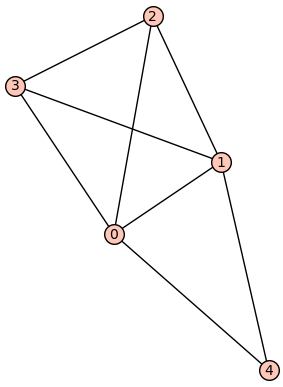
\includegraphics[height=4cm,width=4cm]{graphics/K4+C3-quotient-of-d4reg9h.png}
\end{center}
\end{minipage}
\caption{The quartic graph  $\Gamma_2$ ({\tt d4reg9h}), with a degree two harmonic quotient morphism to the complete house graph, $\Gamma_1=\overline{P_3\cup 2K_1}$.}
\label{fig:harmonic-quotient_d4reg9h-K4+C3}
\end{figure}

}
\end{example}


\begin{example}% d4reg9i
\label{example:d4reg9i}
 {\tt d4reg9i}\newline
{\rm  
Let $\Gamma_2$ denote the graph {\tt d4reg9i} as given above.
There are $5$ harmonic quotient morphisms
$\pi: \Gamma_2\to \Gamma_1=\Gamma_2/G$,
for some subgroup $G$ of $\Aut(\Gamma_2)$.
Two of these are harmonic quotient morphisms to the complete house graph.
The remaining $3$ are harmonic quotient morphisms to the paw graph.
\index{complete house graph}
\index{paw graph}

One of the these harmonic quotient morphisms to the paw graph,
$\pi: \Gamma_2\to \Gamma_1=\Gamma_2/G=\Gamma_1$,
for the subgroup

\[
G = \langle (4,5)(7,8), (0,2)(1,3)(4,7)(5,8) \rangle,
\]
is tabulated below and the morphism is depicted
in Figure \ref{fig:harmonic-quotient_d4reg9i-paw_232311011}.

\begin{center}
\begin{tabular}{c|c|c|c}  
  $x$ & $\phi(x)$ & $m_\phi(x)$ & $\nu_\phi(x)$ \\ \hline
  0   &    2   &        2         &  0   \\ 
  1   &    3   &        2         &  0  \\ 
  2   &    2   &        2         &  0  \\ 
  3   &    3   &        2         &  0  \\ 
  4   &    1   &        1         &  1   \\
  5   &    1   &        1         &  1   \\
  6   &    0   &        4         &  0   \\
  7   &    1   &        1         &  1   \\
  8   &    1   &        1         &  1   \\ 
\end{tabular}
\end{center}

\[
  \genus(\Gamma_2) =10,\ \ \ \ \
  \genus(\Gamma_1) =1,
\]

\[
\deg(\phi) =4.
\]

\begin{figure}[H]
\begin{minipage}{\textwidth}
\begin{center}
%\vspace{8.0 cm}
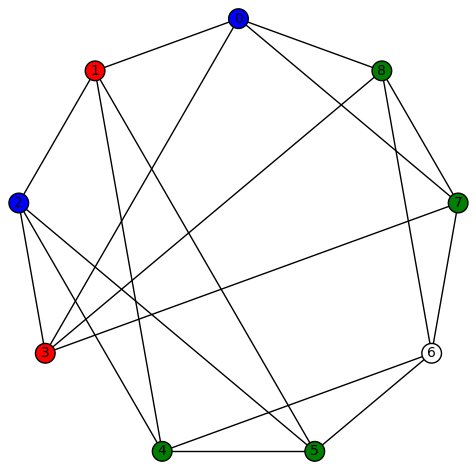
\includegraphics[height=5cm,width=5cm]{graphics/harmonic-quotient_d4reg9i-paw_232311011.png}
\end{center}
\begin{center}
%\vspace{8.0 cm}
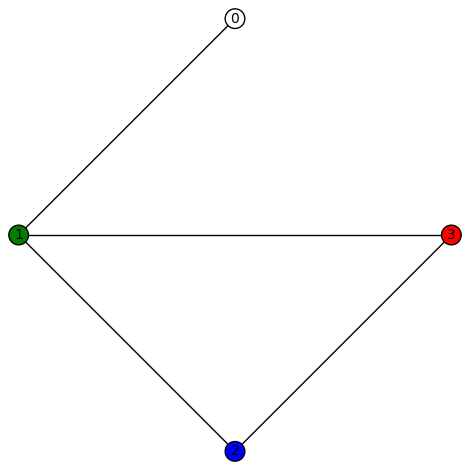
\includegraphics[height=4cm,width=4cm]{graphics/paw_0123.png}
\end{center}
\end{minipage}
\caption{The quartic graph  $\Gamma_2$ ({\tt d4reg9i}), with a degree four harmonic quotient morphism to $\Gamma_1={\rm paw}$.}
\label{fig:harmonic-quotient_d4reg9i-paw_232311011}
\end{figure}
}
\end{example}


\subsection{\texorpdfstring{$10$}{10} vertices}

This subsection describes a selection of the connected quartic graphs on $10$ vertices.
It records their invariants and harmonic morphism counts, and then
works out harmonic quotient morphisms in examples.


There are (up to isomorphism) exactly $59$ $4$-regular connected graphs on $10$ vertices, all of which are Hamiltonian.
Three of these $59$ are vertex transitive,
two of those three are also edge transitive, and one of those two is also distance regular.
Of all these, $17$ have a non-trivial harmonic morphism to $C_3$.
Here, we include only a few examples (including the above-mentioned
vertex transitive graphs), some having a non-trivial harmonic
morphism to $C_3$, some not.


\begin{enumerate}
\item
{\tt d4reg10a}\newline  
Define the graph  $\Gamma$
  % d4reg10-1
  to have edge set:

\[
E = \{
(0, 1), (0, 4), (0, 8), (0, 9), (1, 3), (1, 6), (1, 7), (2, 3), (2, 5), (2, 7), (2, 9),
\]
\[
 (3, 6), (3, 7), (4, 5), (4, 8), (4, 9), (5, 6), (5, 8), (6, 7), (8, 9) 
\}.
\]
It has diameter $3$,
girth $3$, circumference $10$ (i.e., it's Hamiltonian),
critical group of size $27750 = 2\cdot 3\cdot 5^3 37$, 
and automorphism group of size $8$.

There are no non-trivial harmonic morphisms from $\Gamma$ to $P_4$,
$C_3$, $C_4$, or to $K_4$.
However, there are exactly $2$ non-trivial
harmonic morphisms from $\Gamma$ to $P_3$.

\item
  {\tt d4reg10b}\newline  
Define the graph  $\Gamma$
  % d4reg10-6
  to have edge set:

\[
E = \{
(0, 1), (0, 4), (0, 8), (0, 9), (1, 3), (1, 6), (1, 9), (2, 3), (2, 5), (2, 7), (2, 9),
\]
\[
 (3, 7), (3, 8), (4, 5), (4, 8), (4, 9), (5, 6), (5, 7), (6, 7), (6, 8)
\}.
\]
It has diameter $3$,
girth $3$, circumference $10$ (i.e., it's Hamiltonian),
critical group of size $35190 = 2\cdot 3^2 5 \cdot 17\cdot 23$, 
and automorphism group of size $4$.

There are no non-trivial harmonic morphisms from $\Gamma$ to $P_4$, $C_4$,
or to $K_4$.
However, there are exactly $4$ non-trivial
harmonic morphisms from $\Gamma$ to $P_3$
and $12$ non-trivial harmonic morphisms from $\Gamma$ to $C_3$.


\item
  {\tt d4reg10c}\newline  
  Define the graph  $\Gamma$
  % d4reg10-30
  to have edge set:

\[
E = \{
(0, 1), (0, 5), (0, 6), (0, 8), (1, 3), (1, 7), (1, 8), (2, 3), (2, 6), (2, 7), (2, 9),
\]
\[
(3, 4), (3, 9), (4, 5), (4, 8), (4, 9), (5, 6), (5, 9), (6, 7), (7, 8)
\}.
\]
It has diameter $2$,
girth $3$, circumference $10$ (i.e., it's Hamiltonian),
critical group of size $34680 = 2^33\cdot 5\cdot 17^2$, 
and automorphism group of size $2$.

There are no non-trivial harmonic morphisms from $\Gamma$ to $P_3$, $P_4$,
$C_4$, or to $K_4$.
However, there are exactly $6$ non-trivial harmonic morphisms
from $\Gamma$ to $C_3$. 

\item
  {\tt d4reg10d}\newline  
  Define the graph  $\Gamma$
  % d4reg10-34
  to have edge set:

\[
E = \{
(0, 1), (0, 5), (0, 6), (0, 8), (1, 3), (1, 6), (1, 7), (2, 3), (2, 4), (2, 7), (2, 9),
\]
\[
(3, 7), (3, 9), (4, 5), (4, 8), (4, 9), (5, 6), (5, 8), (6, 7), (8, 9)
\}.
\]
It has diameter $3$,
girth $3$, circumference $10$ (i.e., it's Hamiltonian),
critical group of size $30250 = 2\cdot 5^3 11^2$, 
and automorphism group of size $20$ (which acts transitively on the vertex set
but not the edge set).

There are no non-trivial harmonic morphisms from $\Gamma$ to $P_3$
(and therefore $P_k$, $k>3$), $C_3$, $C_4$, or to $K_4$.


\item
  {\tt d4reg10e}\newline  
  Define the graph  $\Gamma$
  % d4reg10-46
  to have edge set:

\[
E = \{
(0, 1), (0, 2), (0, 7), (0, 8), (1, 3), (1, 5), (1, 9), (2, 3), (2, 5), (2, 9),
\]
\[
(3, 4), (3, 6), (4, 5), (4, 7), (4, 8), (5, 6), (6, 7), (6, 8), (7, 9), (8, 9)
\}.
\]
It has diameter $2$,
girth $4$, circumference $10$ (i.e., it's Hamiltonian),
critical group of size $40960 =  2^{13} 5$, 
and automorphism group of size $320$ (which acts transitively on the vertex set {\it and} on the edge set). This is a symmetric (arc transitive) graph
with chromatic number $3$.
It is also a circulant graph with parameters
$(10, [1, 4, 6, 9])$ or with parameters $(10, [2, 3, 7, 8])$.
\index{circulant graph}

There are no non-trivial harmonic morphisms from $\Gamma$ to $C_3$,
$P_4$ (and therefore $P_k$, $k>4$), $K_4$.
There are $40$ non-trivial harmonic morphisms from $\Gamma$ to $P_3$,
$80$ non-trivial harmonic morphisms from $\Gamma$ to $C_4$.

\item
  {\tt d4reg10f}\newline  
  Define the graph  $\Gamma$
  % d4reg10-51
  to have edge set:

\[
E = \{
(0, 1), (0, 2), (0, 5), (0, 8), (1, 3), (1, 4), (1, 7), (2, 3), (2, 7), (2, 9),
\]
\[
(3, 5), (3, 6), (4, 5), (4, 6), (4, 8), (5, 9), (6, 7), (6, 9), (7, 8), (8, 9)
\}.
\]
It has diameter $3$,
girth $4$, circumference $10$ (i.e., it's Hamiltonian),
critical group of size $40500 = 2^2 3^4 5^3$, 
and automorphism group of size $240$ (which acts transitively on the vertex set {\it and} on the edge set). This is a bipartite, symmetric (= arc transitive), distance-regular graph.

There are no non-trivial harmonic morphisms from $\Gamma$ to $P_4$, $C_4$, or to $K_4$.
However, there are exactly $90$ non-trivial harmonic morphisms from $\Gamma$ to $C_3$ and $20$ non-trivial harmonic morphisms from $\Gamma$ to $P_3$.

\end{enumerate}



\subsubsection{Examples}

Each example below takes one graph from the list above and describes
its harmonic quotient morphisms.




\begin{example}% d4reg10a
\label{example:d4reg10a}
 {\tt d4reg10a}\newline
{\rm  
  Let $\Gamma_2$ denote the graph {\tt d4reg10a} as given above.
There are $2$ (not necessarily distinct) harmonic quotient morphisms
$\pi: \Gamma_2\to \Gamma_1=\Gamma_2/G$,
for some $G$. Both are to the $5$ vertex graph $\Gamma_1$
(denoted \verb+D~k+ in graph6 notation)
given by removing an edge from $K_5$.
\index{\verb+D~k+ graph}
An example for
\[
G = \langle (0,1)(2,5)(3,4)(6,9)(7,8) \rangle
\]
is tabulated below and the uncolored graphs are depicted in
Figure \ref{fig:harmonic-quotient_d4reg10a+K5me}.
It is a quasicover.

\begin{center}
\begin{tabular}{c|c|c|c}  
  $x$ & $\phi(x)$ & $m_\phi(x)$ & $\nu_\phi(x)$ \\ \hline
  0   &    2   &        1         &  1   \\ 
  1   &    2   &        1         &  1  \\ 
  2   &    3   &        1         &  1  \\ 
  3   &    0   &        1         &  0  \\ 
  4   &    0   &        1         &  0   \\
  5   &    3   &        1         &  1   \\
  6   &    1   &        1         &  0   \\
  7   &    4   &        1         &  0   \\
  8   &    4   &        1         &  0   \\
  9   &    1   &        1         &  0   \\     
\end{tabular}
\end{center}

\[
  \genus(\Gamma_2) =11,\ \ \ \ \
  \genus(\Gamma_1) =5,
\]

\[
\deg(\phi) =2.
\]

\begin{figure}[H]
\begin{minipage}{\textwidth}
\begin{center}
%\vspace{8.0 cm}
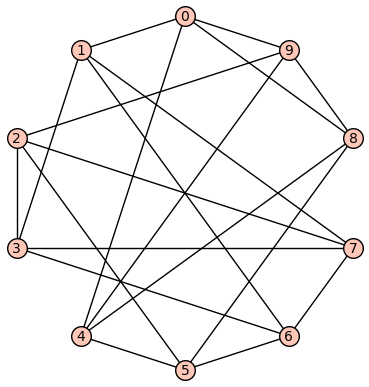
\includegraphics[height=5cm,width=5cm]{graphics/graph_d4reg10a.png}
\end{center}
\begin{center}
%\vspace{8.0 cm}
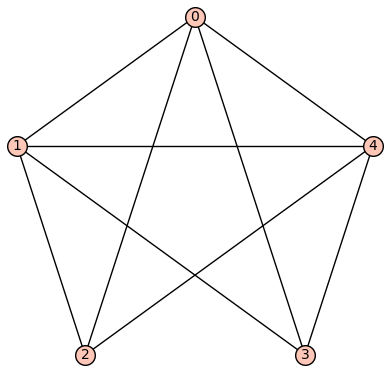
\includegraphics[height=4cm,width=4cm]{graphics/K5me-quotient-of-d4reg10a.png}
\end{center}
\end{minipage}
\caption{The quartic graph $\Gamma_2$ ({\tt d4reg10a}), with a degree two harmonic quotient morphism to the {\tt D\~\,k}$=K_{5}-\{e\}$ graph, $\Gamma_1=\Gamma_2/G$.}
\label{fig:harmonic-quotient_d4reg10a+K5me}
\end{figure}

}
\end{example}



\begin{example}% d4reg10b
\label{example:d4reg10b}
 {\tt d4reg10b}\newline
{\rm  
  Let $\Gamma_2$ denote the graph {\tt d4reg10b} as given above.
There are only $2$ harmonic quotient morphisms
$\pi: \Gamma_2\to \Gamma_1=\Gamma_2/G$, for some $G$.
For $G=\Aut(\Gamma_2)$ (of order $4$) the quotient is $C_3$, with fibers
$\{0,7\}$, $\{1,3,6,8\}$, $\{2,4,5,9\}$.
The other happens to be a quasicover of a wheel graph, as shown below.
\index{wheel graph}
When
\[
G = \langle (0,7)(1,3)(2,9)(4,5)(6,8) \rangle ,
\]
the quotient morphism
$\pi: \Gamma_2\to \Gamma_1=\Gamma_2/G = W_5$
is tabulated below and the uncolored graphs are depicted in
Figure \ref{fig:harmonic-quotient_d4reg10b+W5}.

\begin{center}
\begin{tabular}{c|c|c|c}  
  $x$ & $\phi(x)$ & $m_\phi(x)$ & $\nu_\phi(x)$ \\ \hline
  0   &    1   &        1         &  0   \\ 
  1   &    3   &        1         &  1  \\ 
  2   &    4   &        1         &  1  \\ 
  3   &    3   &        1         &  1  \\ 
  4   &    2   &        1         &  1   \\
  5   &    2   &        1         &  1   \\
  6   &    0   &        1         &  1   \\
  7   &    1   &        1         &  0   \\
  8   &    0   &        1         &  1   \\
  9   &    4   &        1         &  1   \\     
\end{tabular}
\end{center}

\[
  \genus(\Gamma_2) =11,\ \ \ \ \
  \genus(\Gamma_1) =4,
\]
\[
\deg(\phi) =2.
\]

\begin{figure}[H]
\begin{minipage}{\textwidth}
\begin{center}
%\vspace{8.0 cm}
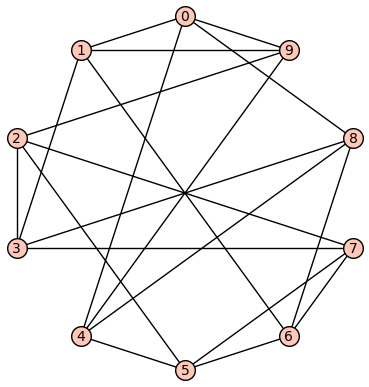
\includegraphics[height=5cm,width=5cm]{graphics/graph_d4reg10b.png}
\end{center}
\begin{center}
%\vspace{8.0 cm}
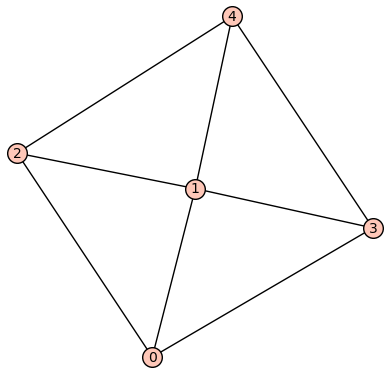
\includegraphics[height=4cm,width=4cm]{graphics/W5-quotient-of-d4reg10b.png}
\end{center}
\end{minipage}
\caption{The quartic graph $\Gamma_2$ ({\tt d4reg10b}), with a degree two harmonic quotient morphism to the wheel graph $W_{5}=\Gamma_1=\Gamma_2/G$.}
\label{fig:harmonic-quotient_d4reg10b+W5}
\end{figure}


}
\end{example}


\begin{example}% d4reg10c
\label{example:d4reg10c}
 {\tt d4reg10c}\newline
{\rm  
  Let $\Gamma_2$ denote the graph {\tt d4reg10c} as given above.
There are no harmonic quotient morphisms
$\pi: \Gamma_2\to \Gamma_1=\Gamma_2/G$,
for some subgroup $G$ of $\Aut(\Gamma_2)$.

}
\end{example}


\begin{example}% d4reg10d
\label{example:d4reg10d}
 {\tt d4reg10d}\newline
{\rm  
  Let $\Gamma_2$ denote the graph {\tt d4reg10d} as given above.
There are $8$ (not necessarily distinct) harmonic quotient morphisms
$\pi: \Gamma_2\to \Gamma_1=\Gamma_2/G$, for some $G$. 

One of these is a cover of a complete graph, as shown below.
\index{complete graph}
When
\[
G = \langle (0,2)(1,4)(3,5)(6,9)(7,8) \rangle ,
\]
the quotient morphism maps to the quartic graph
$\pi: \Gamma_2\to \Gamma_1=\Gamma_2/G = K_5$. This example
is tabulated below and the uncolored graphs are depicted in
Figure \ref{fig:harmonic-quotient_d4reg10d+K5}.

\begin{center}
\begin{tabular}{c|c|c|c}  
  $x$ & $\phi(x)$ & $m_\phi(x)$ & $\nu_\phi(x)$ \\ \hline
  0   &    3   &        1         &  0   \\ 
  1   &    1   &        1         &  0  \\ 
  2   &    3   &        1         &  0  \\ 
  3   &    2   &        1         &  0  \\ 
  4   &    1   &        1         &  0   \\
  5   &    2   &        1         &  0   \\
  6   &    0   &        1         &  0   \\
  7   &    4   &        1         &  0   \\
  8   &    4   &        1         &  0   \\
  9   &    0   &        1         &  0   \\     
\end{tabular}
\end{center}

\[
  \genus(\Gamma_2) =11,\ \ \ \ \
  \genus(\Gamma_1) =6,
\]
\[
\deg(\phi) =2.
\]

\begin{figure}[H]
\begin{minipage}{\textwidth}
\begin{center}
%\vspace{8.0 cm}
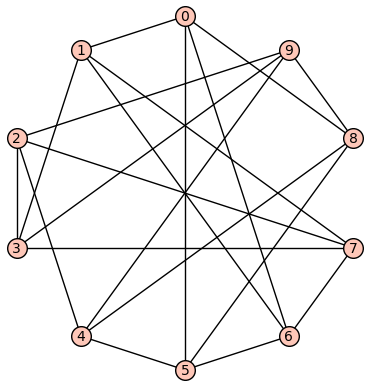
\includegraphics[height=5cm,width=5cm]{graphics/graph_d4reg10d.png}
\end{center}
\begin{center}
%\vspace{8.0 cm}
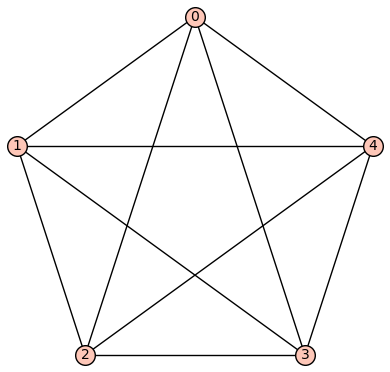
\includegraphics[height=4cm,width=4cm]{graphics/K5-quotient-of-d4reg10d.png}
\end{center}
\end{minipage}
\caption{The quartic graph $\Gamma_2$ ({\tt d4reg10d}), with a degree two harmonic quotient morphism to the quartic graph $K_{5}=\Gamma_1=\Gamma_2/G$.}
\label{fig:harmonic-quotient_d4reg10d+K5}
\end{figure}


Five of the remaining $7$ morphisms are to the 
\verb+EUjo+ graph\footnote{In the graph6 notation.
In the ISGCI notation, it is $\overline{A}$.}.
When
\[
G = \langle (1,8)(3,9)(4,7)(5,6) \rangle ,
\]
the quotient morphism maps to the  graph
$\pi: \Gamma_2\to {\tt EUjo}=\Gamma_1=\Gamma_2/G $. This example
is tabulated below and the uncolored graphs are depicted in
Figure \ref{fig:harmonic-quotient_d4reg10d+barA}.

\begin{center}
\begin{tabular}{c|c|c|c}  
  $x$ & $\phi(x)$ & $m_\phi(x)$ & $\nu_\phi(x)$ \\ \hline
  0   &    4   &        2         &  0   \\ 
  1   &    1   &        1         &  0  \\ 
  2   &    0   &        2         &  0  \\ 
  3   &    3   &        1         &  1  \\ 
  4   &    5   &        1         &  0   \\
  5   &    2   &        1         &  1   \\
  6   &    2   &        1         &  1   \\
  7   &    5   &        1         &  0   \\
  8   &    1   &        1         &  0   \\
  9   &    3   &        1         &  1   \\     
\end{tabular}
\end{center}

\[
  \genus(\Gamma_2) =11,\ \ \ \ \
  \genus(\Gamma_1) =4,
\]
\[
\deg(\phi) =2.
\]

\begin{figure}[H]
\begin{minipage}{\textwidth}
\begin{center}
%\vspace{8.0 cm}
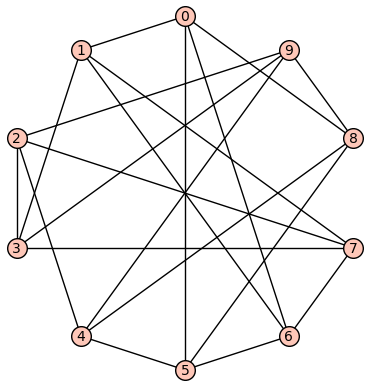
\includegraphics[height=5cm,width=5cm]{graphics/graph_d4reg10d.png}
\end{center}
\begin{center}
%\vspace{8.0 cm}
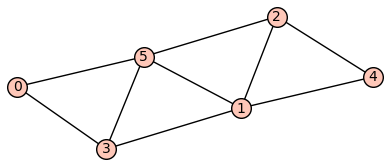
\includegraphics[height=4cm,width=4cm]{graphics/barA-quotient-of-d4reg10d.png}
\end{center}
\end{minipage}
\caption{The quartic graph $\Gamma_2$ ({\tt d4reg10d}), with a degree two harmonic quotient morphism to the graph ${\tt EUjo}=\Gamma_1=\Gamma_2/G$.}
\label{fig:harmonic-quotient_d4reg10d+barA}
\end{figure}

The last two of these harmonic quotient morphisms are to $P_2$ (and are the same morphism).

}
\end{example}


\begin{example}% d4reg10e
\label{example:d4reg10e}
 {\tt d4reg10e}\newline
{\rm  
  Let $\Gamma_2$ denote the graph {\tt d4reg10e} as given above.
There are $850$ harmonic quotient morphisms
$\pi: \Gamma_2\to \Gamma_1=\Gamma_2/G$, for some $G$. 

All $20$ graphs $\Gamma_1$ arising as a quotient with
$6$ vertices are isomorphic to the graph \verb+E@~o+ (in graph6 notation). 

For instance, when
\[
G = \langle  (1,7)(2,8)(3,4)(5,6)\rangle ,
\]
the quotient morphism maps to the  graph
$\pi: \Gamma_2\to $\verb+E@~o+$=\Gamma_1=\Gamma_2/G $. This example
is tabulated below and the uncolored graphs are depicted in
Figure \ref{fig:harmonic-quotient_d4reg10e+E-AT-SIM-o}.

\begin{center}
\begin{tabular}{c|c|c|c}  
  $x$ & $\phi(x)$ & $m_\phi(x)$ & $\nu_\phi(x)$ \\ \hline
  0   &    5   &        2         &  0   \\ 
  1   &    3   &        1         &  0  \\ 
  2   &    1   &        1         &  0  \\ 
  3   &    0   &        1         &  1  \\ 
  4   &    0   &        1         &  1   \\
  5   &    2   &        1         &  1   \\
  6   &    2   &        1         &  1   \\
  7   &    3   &        1         &  0   \\
  8   &    1   &        1         &  0   \\
  9   &    4   &        2         &  0   \\     
\end{tabular}
\end{center}

\[
  \genus(\Gamma_2) =11,\ \ \ \ \
  \genus(\Gamma_1) =4,
\]
\[
\deg(\phi) =2.
\]

\begin{figure}[H]
\begin{minipage}{\textwidth}
\begin{center}
%\vspace{8.0 cm}
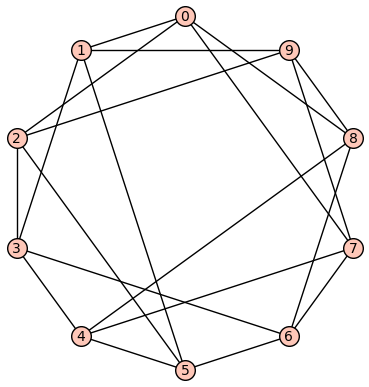
\includegraphics[height=5cm,width=5cm]{graphics/graph_d4reg10e.png}
\end{center}
\begin{center}
%\vspace{8.0 cm}
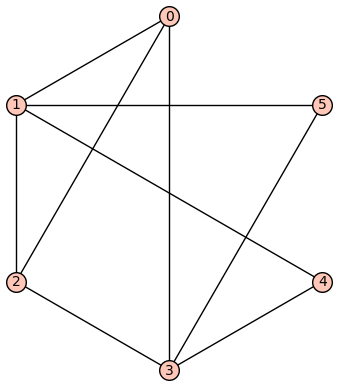
\includegraphics[height=4cm,width=4cm]{graphics/E-AT-SIM-o-quotient-of-d4reg10e.png}
\end{center}
\end{minipage}
\caption{The quartic graph $\Gamma_2$ ({\tt d4reg10e}), with a degree two harmonic quotient morphism to the graph {\tt E@\,\~\,o}$=\Gamma_1=\Gamma_2/G$.}
\label{fig:harmonic-quotient_d4reg10e+E-AT-SIM-o}
\end{figure}


All $158$ graphs $\Gamma_1$ arising as a quotient with
$5$ vertices are isomorphic to the graph $C_5$.

For instance, when
\[
G = \langle  (0,9)(1,2)(3,5)(4,6)(7,8) \rangle ,
\]
the quotient morphism maps to the  graph
$\pi: \Gamma_2\to C_5=\Gamma_1=\Gamma_2/G $.
This multicover example is tabulated below. (All $158$ subgroups with a
$5$-vertex quotient give this same morphism.)

\begin{center}
\begin{tabular}{c|c|c|c}  
  $x$ & $\phi(x)$ & $m_\phi(x)$ & $\nu_\phi(x)$ \\ \hline
  0   &    3   &        2         &  0   \\ 
  1   &    2   &        2         &  0  \\ 
  2   &    2   &        2         &  0  \\ 
  3   &    1   &        2         &  0  \\ 
  4   &    0   &        2         &  0   \\
  5   &    1   &        2         &  0   \\
  6   &    0   &        2         &  0   \\
  7   &    4   &        2         &  0   \\
  8   &    4   &        2         &  0   \\
  9   &    3   &        2         &  0   \\     
\end{tabular}
\end{center}

\[
  \genus(\Gamma_2) =11,\ \ \ \ \
  \genus(\Gamma_1) =1,
\]
\[
\deg(\phi) =4.
\]


All $100$ graphs $\Gamma_1$ arising as a quotient with
$4$ vertices are isomorphic to the graph $C_4$.

All $540$ graphs $\Gamma_1$ arising as a quotient with
$3$ vertices are isomorphic to the graph $P_3$.

All $32$ graphs $\Gamma_1$ arising as a quotient with
$2$ vertices are isomorphic to the graph $P_2$.


}
\end{example}



\begin{example}% d4reg10f
\label{example:d4reg10f}
 {\tt d4reg10f}\newline
{\rm  
  Let $\Gamma_2$ denote the graph {\tt d4reg10f} as given above.
There are $251$ harmonic quotient morphisms
$\pi: \Gamma_2\to \Gamma_1=\Gamma_2/G$, for some $G$. 

One of these $251$ harmonic quotient morphisms is a
cover of the quartic complete graph, $K_5$.
\index{complete graph}
Ten of the remaining $250$ are harmonic quotient morphisms
to a graph isomorphic to $K_5$ minus an edge - the
\verb+D~k+ graph in the graph6 notation.
\index{\verb+D~k+ graph}
Fifteen of the remaining $240$ are harmonic quotient morphisms
to a graph isomorphic to $W_5$, the wheel graph with $5$ vertices.
\index{wheel graph}

Of the remaining $225$, $45$ of the graphs $\Gamma_1$ arise as a quotient with
$3$ vertices isomorphic to the graph $C_3$.

Of the remaining $180$, $30$ of the graphs $\Gamma_1$ arise as a quotient with
$3$ vertices isomorphic to the graph $P_3$.

All of the $150$ remaining graphs $\Gamma_1$ arise as a quotient with
$2$ vertices isomorphic to the graph $P_2$.
}
\end{example}


\subsection{\texorpdfstring{$11$}{11} vertices}

This subsection describes a selection of the connected quartic graphs on $11$ vertices.
It records their invariants and harmonic morphism counts, and then
works out harmonic quotient morphisms in examples.


There are (up to isomorphism) exactly $265$ $4$-regular connected graphs on $11$ vertices. All but one of these are Hamiltonian.
Only two of these are vertex transitive, each with an automorphism group of order $22$, one having critical
group of order $130691 = 11\cdot 109^2$, the other order $87131 = 11\cdot 89^2$.
% d4reg11-82, d4reg11-103

Of all $265$ graphs, only $52$ have a non-trivial harmonic morphism to $C_3$.
This includes an example of a graph having trivial automorphism group, yet $6$ non-trivial harmonic morphisms to $C_3$.
% d4reg11-172

There are $100$ of these $265$ graphs with an odd critical group
(which therefore have no non-trivial harmonic morphisms to $C_4$ or $K_4$).
%Neither of the vertex transitive graphs have any non-trivial harmonic morphisms to $C_3$ or to $C_4$ or to $K_4$.

\begin{enumerate}
\item
  % d4reg11a
 {\tt d4reg11a}\newline
  Define the graph  $\Gamma$
  % d4reg11-3
  to have edge set:

\[
E = \{
(0, 1), (0, 5), (0, 8), (0, 10), (1, 2), (1, 3), (1, 9), (2, 3), (2, 8), (2, 9),
\]
\[
(3, 8), (3, 9), (4, 5), (4, 6), (4, 7), (4, 10), (5, 6), (5, 7), (6, 7),
\]
\[
(6, 10), (7, 10), (8, 9)
\}.
\]
It has diameter $4$,
girth $3$, circumference $6$ (thus not Hamiltonian),
% what is   sage: len(Gamma.longest_path())  ????
critical group of size $40000 = 2^6 5^4$, 
and automorphism group of size $288$. 

There are no non-trivial harmonic morphisms from $\Gamma$ to $P_4$, $C_3$, $C_4$, or to $K_4$. 
However, there are exactly $10$ non-trivial harmonic morphisms from $\Gamma$ to $P_3$. 

\item
  % d4reg11b
 {\tt d4reg11b}\newline
  Define the graph  $\Gamma$
  % d4reg11-8
  to have edge set:

\[
E = \{
(0, 1), (0, 6), (0, 9), (0, 10), (1, 2), (1, 3), (1, 5), (2, 3), (2, 7), (2, 8),
\]
\[
(3, 4), (3, 10), (4, 5), (4, 6), (4, 9), (5, 8), (5, 9), (6, 7), (6, 10),
\]
\[
(7, 8), (7, 10), (8, 9)
\}.
\]
It has diameter $3$,
girth $3$, circumference $11$ (i.e., Hamiltonian),
critical group of size $112404 = 2^2 3 \cdot 17 \cdot 19\cdot 29$, 
and automorphism group of size $2$. 

There are no non-trivial harmonic morphisms from $\Gamma$ to $P_3$, $P_4$, $C_4$, or to $K_4$.
However, there are exactly $6$ non-trivial harmonic morphisms from $\Gamma$ to $C_3$. 


\item
  % d4reg11c
 {\tt d4reg11c}\newline
  Define the graph  $\Gamma$
  % d4reg11-81 or -82
  to have edge set:

\[
E = \{
(0, 1), (0, 2), (0, 9), (0, 10), (1, 3), (1, 5), (1, 7), (2, 3), (2, 4), (2, 7),
\]
\[
(3, 6), (3, 9), (4, 5), (4, 9), (4, 10), (5, 6), (5, 8), (6, 7), (6, 10),
\]
\[
(7, 8), (8, 9), (8, 10)
\}.
\]
It has diameter $2$,
girth $4$, circumference $11$ (i.e., Hamiltonian),
critical group of size $130691 = 11\cdot 109^2$, 
and automorphism group of size $22$. This graph is vertex transitive but not
edge transitive.
\index{vertex transitive graph}

There are no non-trivial harmonic morphisms from $\Gamma$ to $P_3$, $P_4$, $C_3$, $C_4$, or to $K_4$.


\item
  % d4reg11d
 {\tt d4reg11d}\newline
  Define the graph  $\Gamma$
  % d4reg11-102
  to have edge set:

\[
E = \{
(0, 1), (0, 5), (0, 9), (0, 10), (1, 3), (1, 8), (1, 9), (2, 3), (2, 4), (2, 6),
\]
\[
(2, 7), (3, 7),  (3, 8), (4, 5), (4, 6), (4, 10), (5, 6), (5, 10), (6, 7),
\]
\[
(7, 8), (8, 9), (9, 10)
\}.
\]
It has diameter $3$,
girth $3$, circumference $11$ (i.e., Hamiltonian),
critical group of size $87131 = 11\cdot 89^2$, 
and automorphism group of size $22$. This graph is vertex transitive but not
edge transitive.
\index{vertex transitive graph}

There are no non-trivial harmonic morphisms from $\Gamma$ to $P_3$, $P_4$, $C_3$, $C_4$, or to $K_4$.


\item
  % d4reg11e
 {\tt d4reg11e}\newline
  Define the graph  $\Gamma$
  % d4reg11-171 or -172
  to have edge set:

\[
E = \{
(0, 1), (0, 4), (0, 9), (0, 10), (1, 3), (1, 5), (1, 6), (2, 3), (2, 4), (2, 7),
\]
\[
(2, 8), (3, 8), (3, 9), (4, 5), (4, 7), (5, 6), (5, 10), (6, 7), (6, 10),
\]
\[
(7, 8), (8, 9), (9, 10)
\}.
\]
It has diameter $3$,
girth $3$, circumference $11$ (i.e., Hamiltonian),
critical group of size $106056 = 2^3 3^3 491$, 
and automorphism group of size $1$. 

There are no non-trivial harmonic morphisms from $\Gamma$ to $P_3$, $P_4$, $C_4$, or to $K_4$.
However, there are exactly $6$ non-trivial harmonic morphisms from $\Gamma$ to $C_3$. 


\item
  % d4reg11f
 {\tt d4reg11f}\newline
  Define the graph  $\Gamma$
  % d4reg11-13 
  to have edge set:

\[
E = \{
(0, 1), (0, 2), (0, 4), (0, 10), (1, 2), (1, 3), (1, 9), (2, 3), (2, 9), (3, 4), 
\]
\[
(3, 10), (4, 5), (4, 6), (5, 7), (5, 8), (5, 10), (6, 7), (6, 8), (6, 10),
\]
\[
 (7, 8), (7, 9), (8, 9)
\}.
\]
It has diameter $3$,
girth $3$, circumference $11$ (i.e., Hamiltonian),
critical group of size $102400=2^{12} 5^2$, 
and automorphism group of size $64$. 

There are $18$ non-trivial harmonic morphisms from $\Gamma$ to $P_3$ and
none to $P_4$.
Since the diameter is $3$, there are no non-trivial harmonic morphisms
from $\Gamma$ to $P_k$, for $k>4$, by Lemma~\ref{lemma:diameter}.
There are no non-trivial harmonic morphisms from $\Gamma$ to $C_3$ or
to $K_4$, however, there are $16$ non-trivial harmonic morphisms
from $\Gamma$ to $C_4$.


\item
  % d4reg11g
 {\tt d4reg11g}\newline
  Define the graph  $\Gamma$
  % d4reg11-253 
  to have edge set:

\[
E = \{
(0, 1), (0, 8), (0, 9), (0, 10), (1, 3), (1, 4), (1, 6), (2, 3), (2, 4), (2, 6),
\]
\[
 (2, 10), (3, 5), (3, 7), (4, 5), (4, 7), (5, 6), (5, 9), (6, 7),
\]
\[
(7, 8), (8, 9), (8, 10), (9, 10)
\}.
\]
It has diameter $2$,
girth $3$, circumference $11$ (i.e., Hamiltonian),
critical group of size $109744=2^{4} 19^3$, 
and automorphism group of size $144$.

There are $18$ non-trivial harmonic morphisms from $\Gamma$ to $P_3$.
Since the diameter is $2$, there are no non-trivial harmonic morphisms
from $\Gamma$ to $P_k$, for $k>3$, by Lemma~\ref{lemma:diameter}.
There are no non-trivial harmonic morphisms
from $\Gamma$ to $C_4$ or to $K_4$.

\end{enumerate}

% 55, 80, 106, 122, 128, 219, 253, 263 have aut gp >22
% in file3-of-4reg11-graph-data.txt
% 253 has size 144


\subsubsection{Examples}

Each example below takes one graph from the list above and describes
its harmonic quotient morphisms.




\begin{example}% d4reg11a
\label{example:d4reg11a}
 {\tt d4reg11a}\newline
{\rm  
  Let $\Gamma_2$ denote the graph {\tt d4reg11a} as given above.

  There are $12$ harmonic quotient morphisms
$\pi: \Gamma_2\to \Gamma_1=\Gamma_2/G$, for some $G$. 
All of these $12$ (distinct) harmonic quotient morphisms are homomorphisms to the
graph, \verb+EJ~o+ (in the graph6 notation).
\index{\verb+EJ~o+ graph}

For instance, when
\[
G = \langle  (1,5)(2,4)(3,6)(7,9)(8,10)\rangle ,
\]
the quotient morphism maps to the  graph
$\pi: \Gamma_2\to$ {\tt EJ$\sim$o}$=\Gamma_1=\Gamma_2/G $. This example
is tabulated below and the uncolored graphs are depicted in
Figure \ref{fig:harmonic-quotient_d4reg11a+EJ-SIM-o}.

\begin{center}
\begin{tabular}{c|c|c|c}  
  $x$ & $\phi(x)$ & $m_\phi(x)$ & $\nu_\phi(x)$ \\ \hline
  0   &    3   &        2         &  0   \\ 
  1   &    2   &        1         &  0  \\ 
  2   &    1   &        1         &  0  \\ 
  3   &    4   &        1         &  0  \\ 
  4   &    1   &        1         &  0   \\
  5   &    2   &        1         &  0   \\
  6   &    4   &        1         &  0   \\
  7   &    5   &        1         &  0   \\
  8   &    0   &        1         &  0   \\
  9   &    5   &        1         &  0   \\
  10   &   0   &        1         &  0  \\   
\end{tabular}
\end{center}

\[
  \genus(\Gamma_2) =12,\ \ \ \ 
  \genus(\Gamma_1) =6,
\]
\[
\deg(\phi) =2.
\]

\begin{figure}[H]
\begin{minipage}{\textwidth}
\begin{center}
%\vspace{8.0 cm}
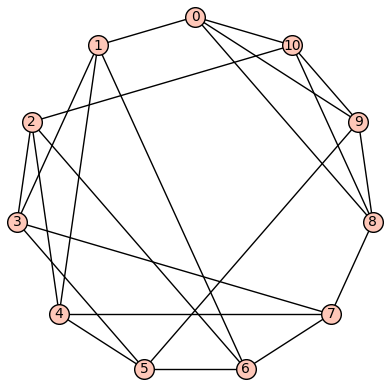
\includegraphics[height=5cm,width=5cm]{graphics/graph_d4reg11a.png}
\end{center}
\begin{center}
%\vspace{8.0 cm}
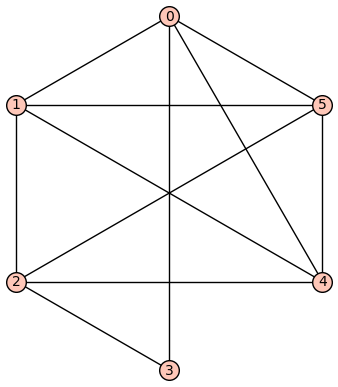
\includegraphics[height=4cm,width=4cm]{graphics/EJ-SIM-o-quotient-of-d4reg11a.png}
\end{center}
\end{minipage}
\caption{The quartic graph $\Gamma_2$ ({\tt d4reg11a}), with a degree two harmonic quotient morphism to the graph {\tt EJ$\sim$o}$=\Gamma_1=\Gamma_2/G$.}
\label{fig:harmonic-quotient_d4reg11a+EJ-SIM-o}
\end{figure}

}
\end{example}


\begin{example}% d4reg11b
\label{example:d4reg11b}
 {\tt d4reg11b}\newline
{\rm  
  Let $\Gamma_2$ denote the graph {\tt d4reg11b} as given above.
There are no harmonic quotient morphisms
$\pi: \Gamma_2\to \Gamma_1=\Gamma_2/G$,
for some subgroup $G$ of $\Aut(\Gamma_2)$.

}
\end{example}



\begin{example}% d4reg11c
\label{example:d4reg11c}
 {\tt d4reg11c}\newline
{\rm  
  Let $\Gamma_2$ denote the graph {\tt d4reg11c} as given above.
There are no harmonic quotient morphisms
$\pi: \Gamma_2\to \Gamma_1=\Gamma_2/G$,
for some subgroup $G$ of $\Aut(\Gamma_2)$.

}
\end{example}


\begin{example}% d4reg11d
\label{example:d4reg11d}
 {\tt d4reg11d}\newline
{\rm  
  Let $\Gamma_2$ denote the graph {\tt d4reg11d} as given above.
There are no harmonic quotient morphisms
$\pi: \Gamma_2\to \Gamma_1=\Gamma_2/G$,
for some subgroup $G$ of $\Aut(\Gamma_2)$.

}
\end{example}


\begin{example}% d4reg11e
\label{example:d4reg11e}
 {\tt d4reg11e}\newline
{\rm  
  Let $\Gamma_2$ denote the graph {\tt d4reg11e} as given above.
There are no harmonic quotient morphisms
$\pi: \Gamma_2\to \Gamma_1=\Gamma_2/G$,
for some subgroup $G$ of $\Aut(\Gamma_2)$.

}
\end{example}




\begin{example}% d4reg11f
\label{example:d4reg11f}
 {\tt d4reg11f}\newline
{\rm  
  Let $\Gamma_2$ denote the graph {\tt d4reg11f} as given above.
There are $30$ harmonic quotient morphisms
$\pi: \Gamma_2\to \Gamma_1=\Gamma_2/G$,
for some subgroup $G$ of $\Aut(\Gamma_2)$.
In some cases, $\Gamma_1$ is a connected graph with $8$ vertices.

Of these $30$, $6$ are (not necessarily distinct)
non-trivial harmonic quotient morphisms
$\pi: \Gamma_2\to \Gamma_1=\Gamma_2/G$, for some $G$, where
$\Gamma_1$ is a graph (depicted below) which we shall
denote\footnote{I tried but could not locate it in the graph6 nor the ISGCI databases.}
$C_6+C_4+C_4$.
For instance, when
\[
G = \langle  (1,2)(4,10)(7,8)\rangle ,
\]
the quotient morphism maps to the  graph
$\pi: \Gamma_2\to \Gamma_1=\Gamma_2/G $. This example
is tabulated below and the uncolored graphs are depicted in
Figure \ref{fig:harmonic-quotient_d4reg11f+C6+C4+C4}.
\index{$C_6+C_4+C_4$ graph}

\begin{center}
\begin{tabular}{c|c|c|c}  
  $x$ & $\phi(x)$ & $m_\phi(x)$ & $\nu_\phi(x)$ \\ \hline
  0   &    7   &        2         &  0   \\ 
  1   &    1   &        1         &  1  \\ 
  2   &    1   &        1         &  1  \\ 
  3   &    4   &        2         &  0  \\ 
  4   &    0   &        1         &  0   \\
  5   &    6   &        2         &  0   \\
  6   &    5   &        2         &  0   \\
  7   &    3   &        1         &  1   \\
  8   &    3   &        1         &  1   \\
  9   &    2   &        2         &  0   \\
  10   &   0   &        1         &  0  \\   
\end{tabular}
\end{center}

\[
  \genus(\Gamma_2) =12,\ \ \ \ \
  \genus(\Gamma_1) =3,
\]
\[
\deg(\phi) =2.
\]

\begin{figure}[H]
\begin{minipage}{\textwidth}
\begin{center}
%\vspace{8.0 cm}
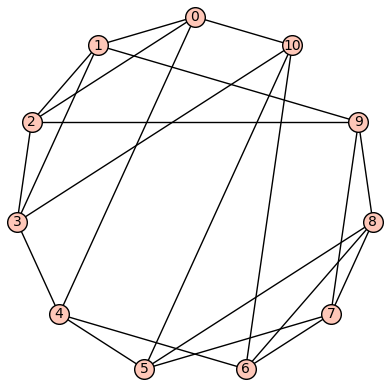
\includegraphics[height=5cm,width=5cm]{graphics/graph_d4reg11f.png}
\end{center}
\begin{center}
%\vspace{8.0 cm}
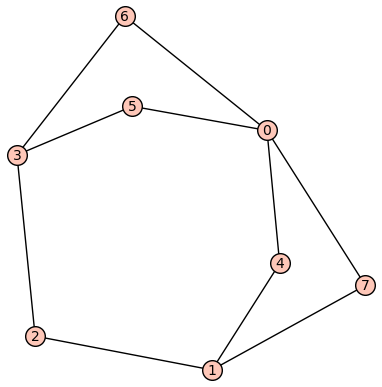
\includegraphics[height=4cm,width=4cm]{graphics/C6+C4+C4-quotient-of-d4reg11f.png}
\end{center}
\end{minipage}
\caption{The quartic graph $\Gamma_2$ ({\tt d4reg11f}), with a degree two harmonic quotient morphism to the graph $C_6+C_4+C_4=\Gamma_1=\Gamma_2/G$.}
\label{fig:harmonic-quotient_d4reg11f+C6+C4+C4}
\end{figure}

Of the remaining $24$, $4$ are (distinct)
non-trivial harmonic quotient morphisms
$\pi: \Gamma_2\to \Gamma_1=\Gamma_2/G$, for some $G$, where
$\Gamma_1$ is the graph (depicted below) denoted
{\tt FCdzo} (in the graph6 database).
For instance, when
\[
G = \langle  (0,5)(1,7)(2,8)(3,6)\rangle ,
\]
the quotient morphism maps to the  graph
$\pi: \Gamma_2\to {\tt FCdzo}=\Gamma_1=\Gamma_2/G $. This example
is tabulated below and the uncolored graphs are depicted in
Figure \ref{fig:harmonic-quotient_d4reg11f+FCdzo}.
This is a homomorphism.
\index{FCdzo graph}

\begin{center}
\begin{tabular}{c|c|c|c}  
  $x$ & $\phi(x)$ & $m_\phi(x)$ & $\nu_\phi(x)$ \\ \hline
  0   &    6   &        1         &  0   \\ 
  1   &    2   &        1         &  0  \\ 
  2   &    1   &        1         &  0  \\ 
  3   &    4   &        1         &  0  \\ 
  4   &    5   &        2         &  0   \\
  5   &    6   &        1         &  0   \\
  6   &    4   &        1         &  0   \\
  7   &    2   &        1         &  0   \\
  8   &    1   &        1         &  0   \\
  9   &    3   &        2         &  0   \\
  10   &   0   &        2         &  0  \\   
\end{tabular}
\end{center}

\[
  \genus(\Gamma_2) =12,\ \ \ \ \
  \genus(\Gamma_1) =5,
\]
\[
\deg(\phi) =2.
\]

\begin{figure}[H]
\begin{minipage}{\textwidth}
\begin{center}
%\vspace{8.0 cm}
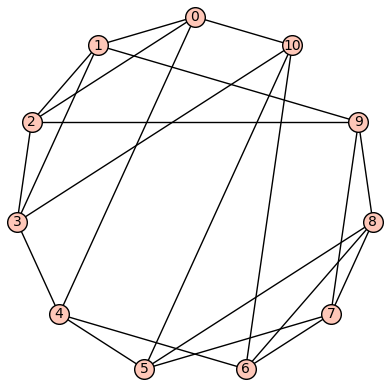
\includegraphics[height=5cm,width=5cm]{graphics/graph_d4reg11f.png}
\end{center}
\begin{center}
%\vspace{8.0 cm}
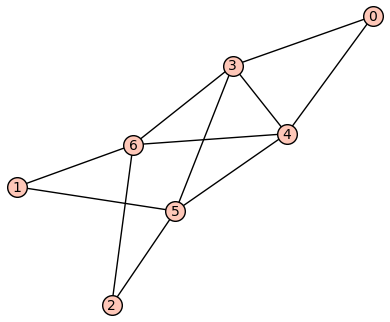
\includegraphics[height=4cm,width=4cm]{graphics/FCdzo-quotient-of-d4reg11f.png}
\end{center}
\end{minipage}
\caption{The quartic graph $\Gamma_2$ ({\tt d4reg11f}), with a degree two harmonic quotient morphism to the graph ${\tt FCdzo}=\Gamma_1=\Gamma_2/G$.}
\label{fig:harmonic-quotient_d4reg11f+FCdzo}
\end{figure}

All of the remaining $20$ are (not necessarily distinct)
non-trivial harmonic quotient morphisms
$\pi: \Gamma_2\to \Gamma_1=\Gamma_2/G$, for some $G$, where
$\Gamma_1$ is the graph (depicted below) denoted
{\tt DrG} (in the graph6 database), also called the {\it banner graph}.
\index{DrG graph}
\index{banner graph}
For instance, when\footnote{Note the
close relationship with this example and the $C_6+C_4+C_4$ example above,
giving us another illustration of composition of quotients.}
\[
G = \langle  (1,2)(4,10)(7,8), (0,5)(1,7)(2,8)(3,6)\rangle ,
\]
the quotient morphism maps to the  graph
$\pi: \Gamma_2\to {\tt DrG}=\Gamma_1=\Gamma_2/G $. This example
is tabulated below and the uncolored graphs are depicted in
Figure \ref{fig:harmonic-quotient_d4reg11f+DrG}. 

\begin{center}
\begin{tabular}{c|c|c|c}  
  $x$ & $\phi(x)$ & $m_\phi(x)$ & $\nu_\phi(x)$ \\ \hline
  0   &    4   &        2         &  0   \\ 
  1   &    3   &        1         &  1  \\ 
  2   &    3   &        1         &  1  \\ 
  3   &    2   &        2         &  0  \\ 
  4   &    0   &        2         &  0   \\
  5   &    4   &        2         &  0   \\
  6   &    2   &        2         &  0   \\
  7   &    3   &        1         &  1   \\
  8   &    3   &        1         &  1   \\
  9   &    1   &        4         &  0   \\
  10   &   0   &        2         &  0  \\   
\end{tabular}
\end{center}

\[
  \genus(\Gamma_2) =12,\ \ \ \ \
  \genus(\Gamma_1) =1,
\]
\[
\deg(\phi) =4.
\]

\begin{figure}[H]
\begin{minipage}{\textwidth}
\begin{center}
%\vspace{8.0 cm}
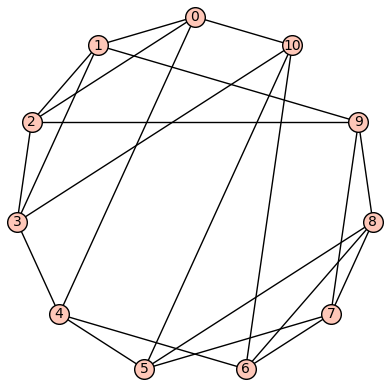
\includegraphics[height=5cm,width=5cm]{graphics/graph_d4reg11f.png}
\end{center}
\begin{center}
%\vspace{8.0 cm}
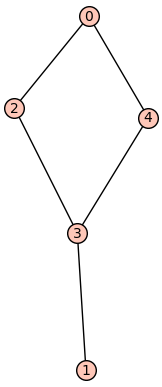
\includegraphics[height=4cm,width=4cm]{graphics/DrG-quotient-of-d4reg11f.png}
\end{center}
\end{minipage}
\caption{The quartic graph $\Gamma_2$ ({\tt d4reg11f}), with a degree four harmonic quotient morphism to the graph ${\tt DrG}=\Gamma_1=\Gamma_2/G$.}
\label{fig:harmonic-quotient_d4reg11f+DrG}
\end{figure}

}
\end{example}
  

\begin{example}% d4reg11g
\label{example:d4reg11g}
 {\tt d4reg11g}\newline
{\rm  
  Let $\Gamma_2$ denote the graph {\tt d4reg11g} as given above.
There are $9$ harmonic quotient morphisms
$\pi: \Gamma_2\to \Gamma_1=\Gamma_2/G$,
for some subgroup $G$ of $\Aut(\Gamma_2)$. In each case,
the quotient graph is the star graph with $5$ vertices:
$\Gamma_1=St_5$.
\index{star graph}

}
\end{example}

\subsection{\texorpdfstring{$12$}{12} vertices}
\label{sec:d4reg12}

This subsection describes a selection of the connected quartic graphs on $12$ vertices.
It records their invariants and harmonic morphism counts, and then
works out harmonic quotient morphisms in examples.


There are (up to isomorphism) exactly $1544$ $4$-regular connected graphs on $12$ vertices. Ten of these are vertex transitive, but only two of those ten are also edge transitive. 


\begin{enumerate}
\item
  % d4reg12a
 {\tt d4reg12a}\newline
  Define the graph  $\Gamma$
  % d4reg12-14
  to have edge set:

\[
E = \{
(0, 1), (0, 2), (0, 7), (0, 10), (1, 3), (1, 5), (1, 6), (2, 3), (2, 9),
\]
\[
(2, 11), (3, 7), (3, 10), (4, 5), (4, 6), (4, 9), (4, 11), (5, 7), (5, 8),
\]
\[
(6, 7), (6, 8), (8, 9), (8, 11), (9, 10), (10, 11)
\}.
\]
It has diameter $3$,
girth $4$, circumference $12$ (i.e., Hamiltonian),
critical group of size $393216 = 2^{17}\cdot 3$, 
and automorphism group of size $768$. This is a vertex transitive and
edge transitive graph. It is also bipartite, symmetric
(= arc transitive), and isomorphic to the circulant graph with
parameters $(12,[1,5])$ or $(12, [1, 5, 7, 11])$.
\index{circulant graph}
\index{vertex transitive graph}
\index{edge transitive graph}
\index{arc transitive graph}
\index{bipartite transitive graph}

There are $6$ non-trivial harmonic
morphisms\footnote{Moreover, it appears all of these are multicovers
  (with constant horizontal multiplicity $2$ and constant vertical
  multiplicity $0$).}
from $\Gamma$ to $C_3$,
$272$ non-trivial harmonic
morphisms\footnote{Moreover, some, but not all, of these are multicovers
  (with constant horizontal multiplicity $2$ and constant vertical
  multiplicity $0$).} from $\Gamma$ to $C_4$,
$82$ non-trivial harmonic morphisms from $\Gamma$ to $P_3$,
$6$ non-trivial harmonic morphisms from $\Gamma$ to $P_4$,
but no non-trivial harmonic morphisms from $\Gamma$ to $K_4$.

\item
  % d4reg12b
 {\tt d4reg12b}\newline
  Define the graph  $\Gamma$
  % d4reg12-47 - 8 to C4, aut gp 24, vert trans, not edge trans
  to have edge set:

\[
E = \{
(0, 1), (0, 5), (0, 7), (0, 10), (1, 3), (1, 6), (1, 10), (2, 3), (2, 4),
\]
\[
(2, 9), (2, 11), (3, 5), (3, 8), (4, 5), (4, 6), (4, 9), (5, 8), (6, 7),
\]
\[
(6, 11), (7, 9), (7, 11), (8, 9), (8, 10), (10, 11)
\}.
\]
It has diameter $3$,
girth $3$, circumference $12$ (i.e., Hamiltonian),
critical group of size $371712 = 2^{10} 3 \cdot 11^2$, 
and automorphism group of size $24$. This is a vertex transitive graph,
but is not edge transitive. It is isomorphic to the circulant graph
having parameters $(12,[1,4])$ or $[(12, [4, 5, 7, 8])$ or
$(12, [1, 4, 8, 11])$.
\index{circulant graph}
\index{vertex transitive graph}

There are $6$ non-trivial harmonic
morphisms\footnote{This is another example where it appears
  all of these are multicovers
  (with constant horizontal multiplicity $2$ and constant vertical
  multiplicity $0$).} from $\Gamma$ to $C_3$,
$8$ non-trivial harmonic
morphisms\footnote{Moreover, it appears all of these are quasicovers
  (with constant horizontal multiplicity $1$ and constant vertical
  multiplicity $2$).}
from $\Gamma$ to $C_4$,
$10$ non-trivial harmonic morphisms from $\Gamma$ to $P_3$.
However, there
are no non-trivial harmonic morphisms from $\Gamma$ to $P_4$ or to $K_4$.
% just the test to K4 took several days!


\item
  
  % d4reg12c
 {\tt d4reg12c}\newline
  Define the graph  $\Gamma$
  % d4reg12-59 
  to have edge set:

\[
E = \{
(0, 1), (0, 2), (0, 7), (0, 10), (1, 3), (1, 5), (1, 11), (2, 3), (2, 9),
\]
\[
 (2, 11), (3, 4), (3, 10), (4, 5), (4, 6), (4, 9), (5, 7), (5, 8),
\]
\[
 (6, 7), (6, 8), (6, 10), (7, 9), (8, 9), (8, 11), (10, 11)
\}.
\]
It has diameter $3$,
girth $4$, circumference $12$ (i.e., Hamiltonian),
critical group of size $405000 = 2^3 3^4 5^4$, 
and automorphism group of size $144$. This is a vertex transitive graph,
but is not edge transitive. It is bipartite.
\index{vertex transitive graph}
\index{bipartite transitive graph}

There are $12$ non-trivial harmonic morphisms from $\Gamma$ to $P_3$
and $36$ non-trivial harmonic morphisms from $\Gamma$ to $C_3$.
However, there are no non-trivial harmonic morphisms
from $\Gamma$ to $P_4$, $C_4$, or to $K_4$.
  
\item
  
  % d4reg12d
 {\tt d4reg12d}\newline
  Define the graph  $\Gamma$
  % d4reg12-195
  to have edge set:

\[
E = \{
(0, 1), (0, 9), (0, 10), (0, 11), (1, 2), (1, 3), (1, 9), (2, 3), (2, 4), 
\]
\[
(2, 11), (3, 5), (3, 8), (4, 5), (4, 6), (4, 11), (5, 6), (5, 8), (6, 7),
\]
\[
(6, 10), (7, 8), (7, 9), (7, 10), (8, 9), (10, 11)
\}.
\]
It has diameter $3$,
girth $3$, circumference $12$,
critical group of size $331776 = 2^{12} 3^4$, 
and automorphism group of size $48$. This is a vertex transitive and
edge transitive graph. It is symmetric, has chromatic number $3$,
and is isomorphic to the cuboctahedron graph.
\index{vertex transitive graph}
\index{cuboctahedron graph}
\index{edge transitive graph}
\index{arc transitive graph}

There are exactly $240$ non-trivial harmonic morphisms from $\Gamma$ to $C_3$,
$20$ non-trivial harmonic morphisms from $\Gamma$ to $P_3$,
$24$ non-trivial harmonic morphisms from $\Gamma$ to $C_4$,
but no non-trivial harmonic morphisms from $\Gamma$ to $P_4$ or to $K_4$.

%It is unknown at this time if there are any non-trivial harmonic morphisms from $\Gamma$ to $K_4$.


\item
  
  % d4reg12e
 {\tt d4reg12e}\newline
  % d4reg12-1269 - 0 to C4, Hamiltonian, aut gp 24, vert trans, not edge trans, circ (12,[2,1])
Define the graph $\Gamma$ to have edge set

\[
E = \{
(0, 1), (0, 3), (0, 10), (0, 11), (1, 5), (1, 9), (1, 10), (2, 3), (2, 6),
\]
\[
 (2, 7), (2, 11), (3, 10), (3, 11), (4, 5), (4, 6), (4, 7), (4, 8),
\]
\[
 (5, 8), (5, 9), (6, 7), (6, 11), (7, 8), (8, 9), (9, 10)
\}.
\]
It has diameter $3$,
girth $3$, circumference $12$,
critical group of size $248832 = 2^{10} 3^5$ (which
equals\footnote{It happens, coincidentally, this formula is in wikipedia
under ``Circulant graph'' but general formulas
for the number of spanning trees in a circulant graph have
been treated by many authors. See for example \cite{MM19} and the
references cited there.} $nF_n^2$, where $n=12$), 
and automorphism group of size $24$. This is a vertex transitive but not
edge transitive graph. It has chromatic number $3$, and is isomorphic to the circulant graph with parameter $(12, [1, 2, 10, 11])$ and
$(12, [2, 5, 7, 10])$.
\index{circulant graph}
\index{vertex transitive graph}

There are $42$ non-trivial harmonic morphisms from $\Gamma$ to $C_3$
and $6$ non-trivial harmonic morphisms from $\Gamma$ to $P_3$.
However, there are no non-trivial harmonic morphisms from $\Gamma$ to $C_4$, $P_4$, or to $K_4$.  

%At this time, it's unknown if this graph has any non-trivial harmonic
%morphisms from $\Gamma$ to $K_4$.

\item
  % d4reg12f
 {\tt d4reg12f}\newline
  % d4reg12-1537 - 48 to C4, bipartite, aut gp 64,
Define the graph $\Gamma$ to have edge set

\[
E = \{
(0, 1), (0, 2), (0, 4), (0, 8), (1, 3), (1, 5), (1, 6), (2, 3), (2, 5), (2, 9),
\]
\[
(3, 7), (3, 11), (4, 5), (4, 6), (4, 10), (5, 8), (6, 7), (6, 11), 
\]
\[
(7, 9), (7, 10), (8, 9), (8, 10), (9, 11), (10, 11)
\}.
\]
It has diameter $3$,
girth $4$, circumference $12$,
critical group of size $401408 = 2^{13} 7^2$, 
and automorphism group of size $64$. This is a bipartite graph.

There are $48$ non-trivial harmonic morphisms from $\Gamma$ to $C_4$,
$32$ non-trivial harmonic morphisms from $\Gamma$ to $P_3$,
$2$ non-trivial harmonic morphisms from $\Gamma$ to $P_4$, but
there are no non-trivial harmonic morphisms from $\Gamma$ to $C_3$
or to $K_4$.

%At this time, it's unknown if this graph has any non-trivial harmonic
%morphisms from $\Gamma$ to $K_4$.

\end{enumerate}



\subsubsection{Examples}

Each example below takes one graph from the list above and describes
its harmonic quotient morphisms.




\begin{example}% d4reg12a
\label{example:d4reg12a}  
 {\tt d4reg12a}\newline
{\rm  
Let $\Gamma_2$ denote the graph {\tt d4reg12a} as given above.
This graph, because of its large automorphism group, has a lot of
graph quotients. In fact, it has
$7195$  non-trivial harmonic quotient morphisms
$\pi: \Gamma_2\to \Gamma_1=\Gamma_2/G$,
for some subgroup $G$ of $\Aut(\Gamma_2)$.

There are $12$ in the case $\Gamma_1$ has $9$ vertices,
$12$ in the case $\Gamma_1$ has $8$ vertices,
$1482$ in the case $\Gamma_1$ has $6$ vertices,
$2294$ in the case $\Gamma_1$ has $4$ vertices,
$1634$ in the case $\Gamma_1$ has $3$ vertices,
and  $1761$ in the case $\Gamma_1$ has $2$ vertices
(i.e., $\Gamma_1=P_2$).

For instance, when
\[
G = \langle  (1,7)(2,10)(4,8) \rangle ,
\]
the quotient morphism maps to the graph
$\pi: \Gamma_2\to $\verb+H??E\hw+$=\Gamma_1=\Gamma_2/G $ (in graph6 notation).
All of the $12$ quotients $\Gamma_1=\Gamma_2/G$ having $9$ vertices
are isomorphic to this graph, \verb+H??E\hw+.
This example
is tabulated below and the uncolored graphs are depicted in
Figure \ref{fig:harmonic-quotient_d4reg12a+v9e12ds444222222}. 
Note this is a graph homomorphism.

\begin{center}
\begin{tabular}{c|c|c|c}  
  $x$ & $\phi(x)$ & $m_\phi(x)$ & $\nu_\phi(x)$ \\ \hline
  0   &    8   &        2         &  0   \\ 
  1   &    2   &        1         &  0  \\ 
  2   &    1   &        1         &  0  \\ 
  3   &    4   &        2         &  0  \\ 
  4   &    7   &        1         &  0   \\
  5   &    6   &        2         &  0   \\
  6   &    5   &        2         &  0   \\
  7   &    2   &        1         &  0   \\
  8   &    7   &        1         &  0   \\
  9   &    3   &        2         &  0   \\
  10   &   1   &        1         &  0  \\   
  11   &   0   &        2         &  0  \\
\end{tabular}
\end{center}

\[
  \genus(\Gamma_2) =13,\ \ \ \ \
  \genus(\Gamma_1) =4,
\]
\[
\deg(\phi) =2.
\]

\begin{figure}[H]
\begin{minipage}{\textwidth}
\begin{center}
%\vspace{8.0 cm}
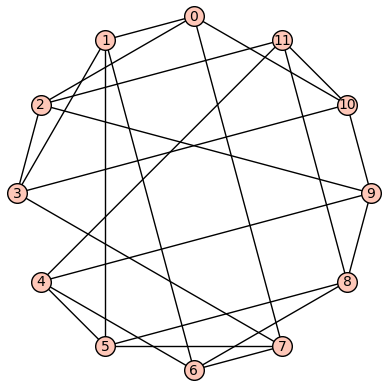
\includegraphics[height=5cm,width=5cm]{graphics/graph_d4reg12a.png}
\end{center}
\begin{center}
%\vspace{8.0 cm}
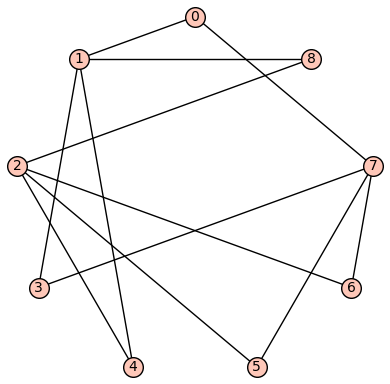
\includegraphics[height=4cm,width=4cm]{graphics/v9e12ds444222222-quotient-of-d4reg12a.png}
\end{center}
\end{minipage}
\caption{The quartic graph $\Gamma_2$ ({\tt d4reg12a}), with a degree two harmonic quotient morphism to the $9$ vertex graph $\Gamma_1=\Gamma_2/G$ described above.}
\label{fig:harmonic-quotient_d4reg12a+v9e12ds444222222}
\end{figure}

% v8e12ds44442222 = G?r@xw
For instance, when
\[
G = \langle  (1,2)(5,9)(6,11)(7,10) \rangle ,
\]
the quotient morphism maps to the graph
$\pi: \Gamma_2\to $\verb+G?r@xw+$=\Gamma_1=\Gamma_2/G $ (in graph6 notation).
All of the $12$ quotients $\Gamma_1=\Gamma_2/G$ having $8$ vertices
are isomorphic to this graph, \verb+G?r@xw+.
This example
is tabulated below and the uncolored graphs are depicted in
Figure \ref{fig:harmonic-quotient_d4reg12a+v8e12ds44442222}. 
Note this is a graph homomorphism.

\begin{center}
\begin{tabular}{c|c|c|c}  
  $x$ & $\phi(x)$ & $m_\phi(x)$ & $\nu_\phi(x)$ \\ \hline
  0   &    7   &        2         &  0   \\ 
  1   &    0   &        1         &  0  \\ 
  2   &    0   &        1         &  0  \\ 
  3   &    4   &        2         &  0  \\ 
  4   &    6   &        2         &  0   \\
  5   &    5   &        1         &  0   \\
  6   &    3   &        1         &  0   \\
  7   &    1   &        1         &  0   \\
  8   &    2   &        2         &  0   \\
  9   &    5   &        1         &  0   \\
  10   &   1   &        1         &  0  \\   
  11   &   3   &        1         &  0  \\
\end{tabular}
\end{center}

\[
  \genus(\Gamma_2) =13,\ \ \ \ \
  \genus(\Gamma_1) =5,
\]
\[
\deg(\phi) =2.
\]

\begin{figure}[H]
\begin{minipage}{\textwidth}
\begin{center}
%\vspace{8.0 cm}
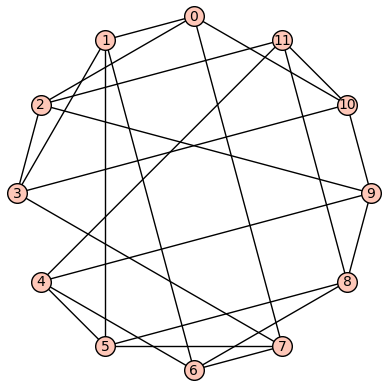
\includegraphics[height=5cm,width=5cm]{graphics/graph_d4reg12a.png}
\end{center}
\begin{center}
%\vspace{8.0 cm}
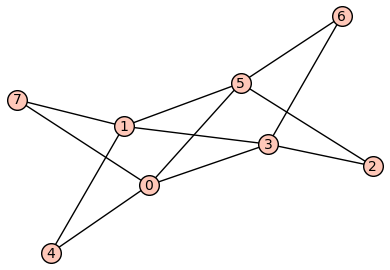
\includegraphics[height=4cm,width=4cm]{graphics/v8e12ds44442222-quotient-of-d4reg12a.png}
\end{center}
\end{minipage}
\caption{The quartic graph $\Gamma_2$ ({\tt d4reg12a}), with a degree two harmonic quotient morphism to the $8$ vertex graph $\Gamma_1=\Gamma_2/G$ described above.}
\label{fig:harmonic-quotient_d4reg12a+v8e12ds44442222}
\end{figure}

For instance, when
\[
G = \langle (0,3)(1,7)(2,10)(4,8)(5,6)(9,11) \rangle ,
\]
the quotient morphism maps (is a $2$-multicover, in fact) to the cycle graph
$\pi: \Gamma_2\to C_6=\Gamma_1=\Gamma_2/G $.
Of the $1482$ quotients $\Gamma_1=\Gamma_2/G$ having $6$ vertices,
$1330$ are isomorphic to this cycle graph $C_6$ (and all $1330$ give this
same morphism). The others are $120$ quotients to $C_4$ with two pendant
edges at one vertex, $24$ to $\overline{C_4\cup K_2}$, and $8$ to the
octahedral graph.
This example
is tabulated below and the uncolored graphs are depicted in
Figure \ref{fig:harmonic-quotient_d4reg12a+C6}. 

\begin{center}
\begin{tabular}{c|c|c|c}  
  $x$ & $\phi(x)$ & $m_\phi(x)$ & $\nu_\phi(x)$ \\ \hline
  0   &    4   &        2         &  0   \\ 
  1   &    3   &        2         &  0  \\ 
  2   &    2   &        2         &  0  \\ 
  3   &    4   &        2         &  0  \\ 
  4   &    5   &        2         &  0   \\
  5   &    0   &        2         &  0   \\
  6   &    0   &        2         &  0   \\
  7   &    3   &        2         &  0   \\
  8   &    5   &        2         &  0   \\
  9   &    1   &        2         &  0   \\
  10   &   2   &        2         &  0  \\   
  11   &   1   &        2         &  0  \\
\end{tabular}
\end{center}

\[
  \genus(\Gamma_2) =13,\ \ \ \ \
  \genus(\Gamma_1) =1,
\]
\[
\deg(\phi) =4.
\]

\begin{figure}[H]
\begin{minipage}{\textwidth}
\begin{center}
%\vspace{8.0 cm}
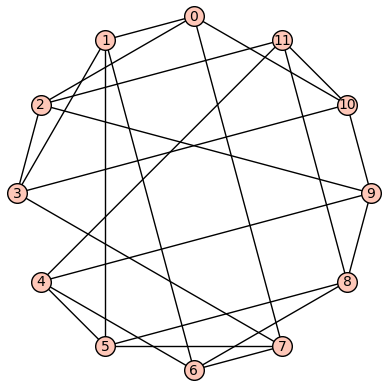
\includegraphics[height=5cm,width=5cm]{graphics/graph_d4reg12a.png}
\end{center}
\begin{center}
%\vspace{8.0 cm}
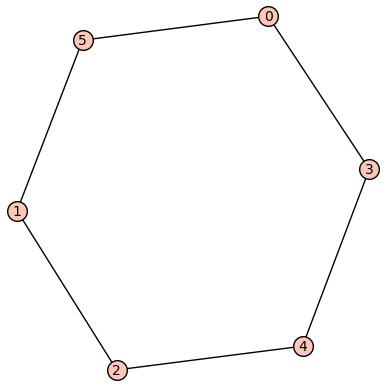
\includegraphics[height=4cm,width=4cm]{graphics/C6-quotient-of-d4reg12a.png}
\end{center}
\end{minipage}
\caption{The quartic graph $\Gamma_2$ ({\tt d4reg12a}), with a degree four harmonic quotient morphism to the graph $C_6=\Gamma_1=\Gamma_2/G$ described above.}
\label{fig:harmonic-quotient_d4reg12a+C6}
\end{figure}

For instance, when
\[
G = \langle (0,5,9)(1,4,2)(3,6,11)(7,8,10) \rangle ,
\]
the quotient morphism maps (is a $2$-multicover, in fact) to the cycle graph
$\pi: \Gamma_2\to C_4=\Gamma_1=\Gamma_2/G $.
Of the $2294$ quotients $\Gamma_1=\Gamma_2/G$ having $4$ vertices,
$170$ are isomorphic to this cycle graph $C_4$, $48$ to the diamond graph,
and $2076$ to the path graph $P_4$.
This example
is tabulated below and the uncolored graphs are depicted in
Figure \ref{fig:harmonic-quotient_d4reg12a+C4}. 

\begin{center}
\begin{tabular}{c|c|c|c}  
  $x$ & $\phi(x)$ & $m_\phi(x)$ & $\nu_\phi(x)$ \\ \hline
  0   &    2   &        2         &  0   \\ 
  1   &    0   &        2         &  0  \\ 
  2   &    0   &        2         &  0  \\ 
  3   &    3   &        2         &  0  \\ 
  4   &    0   &        2         &  0   \\
  5   &    2   &        2         &  0   \\
  6   &    3   &        2         &  0   \\
  7   &    1   &        2         &  0   \\
  8   &    1   &        2         &  0   \\
  9   &    2   &        2         &  0   \\
  10   &   1   &        2         &  0  \\   
  11   &   3   &        2         &  0  \\
\end{tabular}
\end{center}

\[
  \genus(\Gamma_2) =13,\ \ \ \ \
  \genus(\Gamma_1) =1,
\]
\[
\deg(\phi) =6.
\]

\begin{figure}[H]
\begin{minipage}{\textwidth}
\begin{center}
%\vspace{8.0 cm}
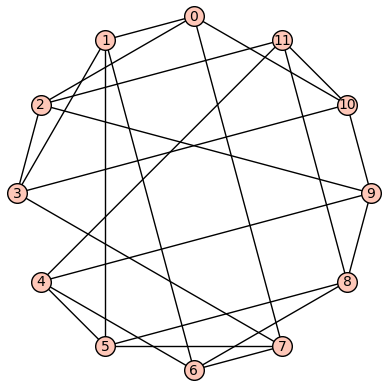
\includegraphics[height=5cm,width=5cm]{graphics/graph_d4reg12a.png}
\end{center}
\begin{center}
%\vspace{8.0 cm}
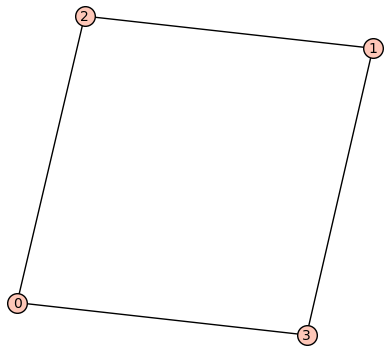
\includegraphics[height=4cm,width=4cm]{graphics/C4-quotient-of-d4reg12a.png}
\end{center}
\end{minipage}
\caption{The quartic graph $\Gamma_2$ ({\tt d4reg12a}), with a degree six harmonic quotient morphism to the graph $C_4=\Gamma_1=\Gamma_2/G$ described above.}
\label{fig:harmonic-quotient_d4reg12a+C4}
\end{figure}

Of the $1634$ quotients $\Gamma_1=\Gamma_2/G$ having $3$ vertices,
$1309$ are isomorphic to the path graph $P_3$ and $325$ to the cycle graph $C_3$.

All of the $1761$ quotients $\Gamma_1=\Gamma_2/G$ having $2$ vertices
are isomorphic to the path graph $P_2$.
}
\end{example}



\begin{example}% d4reg12b
\label{example:d4reg12b}
 {\tt d4reg12b}\newline
{\rm  
  Let $\Gamma_2$ denote the graph {\tt d4reg12b} as given above.
It has $21$  non-trivial harmonic quotient morphisms
$\pi: \Gamma_2\to \Gamma_1=\Gamma_2/G$,
for some subgroup $G$ of $\Aut(\Gamma_2)$.
There are $6$ in the case $\Gamma_1$ has $7$ vertices,
only $1$ in the case $\Gamma_1$ has $6$ vertices,
$4$ in the case $\Gamma_1$ has $4$ vertices,
$3$ in the case $\Gamma_1$ has $3$ vertices,
and  $7$ in the case $\Gamma_1$ has $2$ vertices
(i.e., $\Gamma_1=P_2$).


For instance, when
\[
G = \langle (1,10)(3,11)(4,9)(5,7)(6,8) \rangle ,
\]
the quotient morphism $\pi$ maps to the $7$ vertex graph
$\pi: \Gamma_2\to {\tt FKMiw}=\Gamma_1=\Gamma_2/G $ (in the graph6 notation).
In fact, every harmonic quotient having $7$ vertices is isomorphic to
this graph. This example
is tabulated below and the uncolored graphs are depicted in
Figure \ref{fig:harmonic-quotient_d4reg12b+FKMiw}. 

\begin{center}
\begin{tabular}{c|c|c|c}  
  $x$ & $\phi(x)$ & $m_\phi(x)$ & $\nu_\phi(x)$ \\ \hline
  0   &    2   &        2         &  0   \\ 
  1   &    5   &        1         &  1  \\ 
  2   &    0   &        2         &  0  \\ 
  3   &    4   &        1         &  0  \\ 
  4   &    3   &        1         &  1   \\
  5   &    6   &        1         &  0   \\
  6   &    1   &        1         &  0   \\
  7   &    6   &        1         &  0   \\
  8   &    1   &        1         &  0   \\
  9   &    3   &        1         &  1   \\
  10   &   5   &        1         &  1  \\   
  11   &   4   &        1         &  0  \\
\end{tabular}
\end{center}

\[
  \genus(\Gamma_2) =13,\ \ \ \ \
  \genus(\Gamma_1) =5,
\]
\[
\deg(\phi) =2.
\]

\begin{figure}[H]
\begin{minipage}{\textwidth}
\begin{center}
%\vspace{8.0 cm}
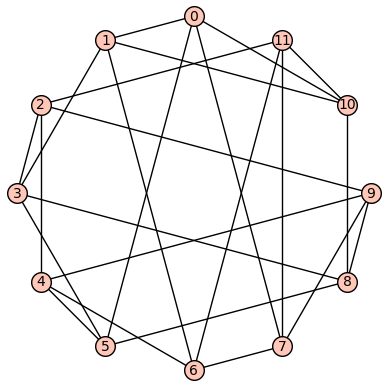
\includegraphics[height=5cm,width=5cm]{graphics/graph_d4reg12b.png}
\end{center}
\begin{center}
%\vspace{8.0 cm}
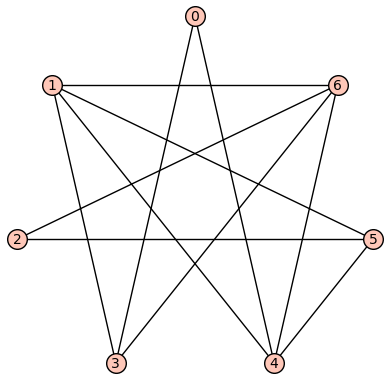
\includegraphics[height=4cm,width=4cm]{graphics/FKMiw-quotient-of-d4reg12b.png}
\end{center}
\end{minipage}
\caption{The quartic graph $\Gamma_2$ ({\tt d4reg12b}), with a degree two harmonic quotient morphism to the graph {\tt FKMiw}$=\Gamma_1=\Gamma_2/G$ described above.}
\label{fig:harmonic-quotient_d4reg12b+FKMiw}
\end{figure}


For instance, when
\[
G = \langle (0,2)(1,9)(3,7)(4,10)(5,11)(6,8) \rangle ,
\]
the quotient morphism $\pi$ maps (as a cover, in fact) to the quartic graph
$\pi: \Gamma_2\to $\verb+E]~o+$=\Gamma_1=\Gamma_2/G$ (in the graph6 notation).
In fact, this graph \verb+E]~o+ is a circulant graph with parameters
$(6, [1, 2, 4, 5])$. This example
is tabulated below and the uncolored graphs are depicted in
Figure \ref{fig:harmonic-quotient_d4reg12b+circ6-1245}.
\index{circulant graph}
  
\begin{center}
\begin{tabular}{c|c|c|c}  
  $x$ & $\phi(x)$ & $m_\phi(x)$ & $\nu_\phi(x)$ \\ \hline
  0   &    5   &        1         &  0   \\ 
  1   &    2   &        1         &  0  \\ 
  2   &    5   &        1         &  0  \\ 
  3   &    4   &        1         &  0  \\ 
  4   &    0   &        1         &  0   \\
  5   &    1   &        1         &  0   \\
  6   &    3   &        1         &  0   \\
  7   &    4   &        1         &  0   \\
  8   &    3   &        1         &  0   \\
  9   &    2   &        1         &  0   \\
  10   &   0   &        1         &  0  \\   
  11   &   1   &        1         &  0  \\
\end{tabular}
\end{center}

\[
  \genus(\Gamma_2) = 13,\ \ \ \ \
  \genus(\Gamma_1) = 7,
\]
\[
\deg(\phi) =2.
\]

\begin{figure}[H]
\begin{minipage}{\textwidth}
\begin{center}
%\vspace{8.0 cm}
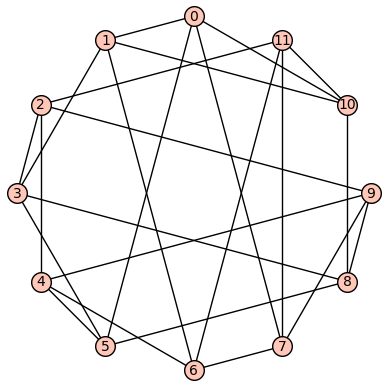
\includegraphics[height=5cm,width=5cm]{graphics/graph_d4reg12b.png}
\end{center}
\begin{center}
%\vspace{8.0 cm}
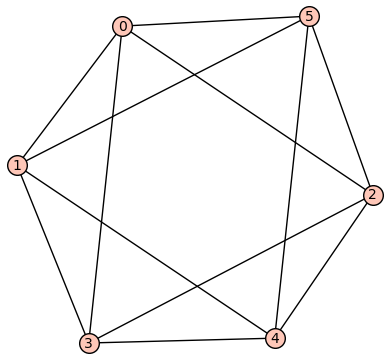
\includegraphics[height=4cm,width=4cm]{graphics/circ6-1245-quotient-of-d4reg12b.png}
\end{center}
\end{minipage}
\caption{The quartic graph $\Gamma_2$ ({\tt d4reg12b}), with a degree two harmonic quotient morphism to the circulant graph $\Gamma_1=\Gamma_2/G$ described above.}
\label{fig:harmonic-quotient_d4reg12b+circ6-1245}
\end{figure}

For instance, when
\[
G = \langle (0,1,10)(2,9,4)(3,8,5)(6,11,7) \rangle ,
\]
the quotient morphism $\pi$ maps to the $4$ vertex graph
$\pi: \Gamma_2\to C_4=\Gamma_1=\Gamma_2/G $.
In fact, every harmonic quotient having $4$ vertices is isomorphic to
either this graph $C_4$ or to the diamond graph. This $C_4$ example
is tabulated below.
% and the uncolored graphs are depicted in
% Figure \ref{fig:harmonic-quotient_d4reg12b+C4}. 

\begin{center}
\begin{tabular}{c|c|c|c}  
  $x$ & $\phi(x)$ & $m_\phi(x)$ & $\nu_\phi(x)$ \\ \hline
  0   &    1   &        1         &  2   \\ 
  1   &    1   &        1         &  2  \\ 
  2   &    2   &        1         &  2  \\ 
  3   &    3   &        1         &  2  \\ 
  4   &    2   &        1         &  2   \\
  5   &    3   &        1         &  2   \\
  6   &    0   &        1         &  2   \\
  7   &    0   &        1         &  2   \\
  8   &    3   &        1         &  2   \\
  9   &    2   &        1         &  2   \\
  10   &   1   &        1         &  2  \\   
  11   &   0   &        1         &  2  \\
\end{tabular}
\end{center}

\[
  \genus(\Gamma_2) =13,\ \ \ \ \
  \genus(\Gamma_1) =1,
\]
\[
\deg(\phi) =3.
\]

In fact, every harmonic quotient having $3$ vertices is isomorphic to
either $P_3$ (two of them) or $C_3$ (one of them).

Of course, every one of the $7$ harmonic quotients $\Gamma_1$ having $2$
vertices is isomorphic to $P_2$.

}
\end{example}



\begin{example}% d4reg12c
\label{example:d4reg12c}
 {\tt d4reg12c}\newline
{\rm  
  Let $\Gamma_2$ denote the graph {\tt d4reg12c} as given above.
It has $142$  non-trivial harmonic quotient morphisms
$\pi: \Gamma_2\to \Gamma_1=\Gamma_2/G$,
for some subgroup $G$ of $\Aut(\Gamma_2)$.
There are $22$ in the case $\Gamma_1$ has $6$ vertices,
$6$ in the case $\Gamma_1$ has $4$ vertices,
$6$ in the case $\Gamma_1$ has $3$ vertices,
and  $108$ in the case $\Gamma_1$ has $2$ vertices
(i.e., $\Gamma_1=P_2$).

For those quotients having $6$ vertices, the following graphs arise
(in graph6 notation): \verb+ELv_+ (= the prism graph),
\verb+EFz_+ (= $K_{3,3}$), \verb+Ejmw+, \verb+Es\w+. 
\index{prism graph}
\index{complete bipartite graph}

For instance, when
\[
G = \langle (0,1)(2,3)(4,9)(5,7)(6,8)(10,11) \rangle ,
\]
the quotient morphism $\pi$ (a quasicover) maps to the $6$ vertex prism graph
$\pi: \Gamma_2\to \Gamma_1=\Gamma_2/G $, as tabulated below.

\begin{center}
\begin{tabular}{c|c|c|c}  
  $x$ & $\phi(x)$ & $m_\phi(x)$ & $\nu_\phi(x)$ \\ \hline
  0   &    3   &        1         &  1   \\ 
  1   &    3   &        1         &  1  \\ 
  2   &    1   &        1         &  1  \\ 
  3   &    1   &        1         &  1  \\ 
  4   &    2   &        1         &  1   \\
  5   &    5   &        1         &  1   \\
  6   &    0   &        1         &  1   \\
  7   &    5   &        1         &  1   \\
  8   &    0   &        1         &  1   \\
  9   &    2   &        1         &  1   \\
  10   &   4   &        1         &  1  \\   
  11   &   4   &        1         &  1  \\
\end{tabular}
\end{center}

\[
  \genus(\Gamma_2) =13,\ \ \ \ \
  \genus(\Gamma_1) =4,
\]
\[
\deg(\phi) =2.
\]

If you replace one of the rectangular faces (a $C_4$)
of the prism graph with a copy of $K_4$, then you get the
graph denoted {\tt Ejmw} (in the graph6 notation).
For instance, when
\[
G = \langle (0,4)(1,5)(2,6)(3,7)(8,11)(9,10) \rangle ,
\]
the quotient morphism $\pi$ (a quasicover) maps to the $6$ vertex graph {\tt Ejmw}
$\pi: \Gamma_2\to \Gamma_1=\Gamma_2/G $, as tabulated below.
The uncolored graphs are depicted in
Figure \ref{fig:harmonic-quotient_d4reg12c+Ejmw}. 

\begin{center}
\begin{tabular}{c|c|c|c}  
  $x$ & $\phi(x)$ & $m_\phi(x)$ & $\nu_\phi(x)$ \\ \hline
  0   &    5   &        1         &  0   \\ 
  1   &    1   &        1         &  1  \\ 
  2   &    4   &        1         &  0  \\ 
  3   &    3   &        1         &  0  \\ 
  4   &    5   &        1         &  0   \\
  5   &    1   &        1         &  1   \\
  6   &    4   &        1         &  0   \\
  7   &    3   &        1         &  0   \\
  8   &    0   &        1         &  1   \\
  9   &    2   &        1         &  0   \\
  10   &   2   &        1         &  0  \\   
  11   &   0   &        1         &  1  \\
\end{tabular}
\end{center}

\[
  \genus(\Gamma_2) =13,\ \ \ \ \
  \genus(\Gamma_1) =6,
\]
\[
\deg(\phi) =2.
\]

\begin{figure}[H]
\begin{minipage}{\textwidth}
\begin{center}
%\vspace{8.0 cm}
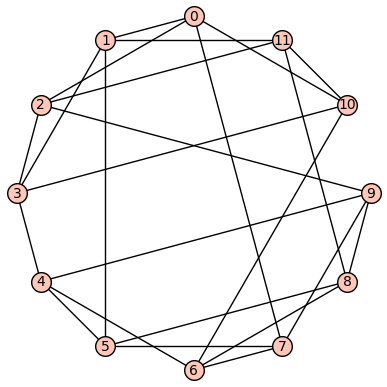
\includegraphics[height=5cm,width=5cm]{graphics/graph_d4reg12c.png}
\end{center}
\begin{center}
%\vspace{8.0 cm}
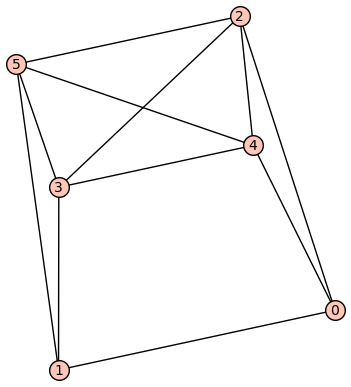
\includegraphics[height=4cm,width=4cm]{graphics/Ejmw-quotient-of-d4reg12c.png}
\end{center}
\end{minipage}
\caption{The quartic graph $\Gamma_2$ ({\tt d4reg12c}), with a degree two harmonic quotient morphism (indeed, a quasicover) to the graph {\tt Ejmw}$=\Gamma_1=\Gamma_2/G$ described above.}
\label{fig:harmonic-quotient_d4reg12c+Ejmw}
\end{figure}

All $6$ of the non-trivial harmonic quotient morphisms
$\pi: \Gamma_2\to \Gamma_1=\Gamma_2/G$, in the case where
$\Gamma_1$ has $4$ vertices, satisfy $\Gamma_1=St_4$.
\index{star graph}

All $6$ of the non-trivial harmonic quotient morphisms
$\pi: \Gamma_2\to \Gamma_1=\Gamma_2/G$, in the case where
$\Gamma_1$ has $3$ vertices, satisfy $\Gamma_1=C_3$.
In fact, all these morphisms are quasicovers.
For instance, when
\[
G = \langle  (0,1)(2,3)(4,9)(5,7)(6,8)(10,11),
(0,7)(1,5)(2,9)(3,4)(6,10)(8,11)\rangle ,
\]
the quotient morphism $\pi$ (a quasicover) maps to the cycle graph
$\pi: \Gamma_2\to C_3=\Gamma_1=\Gamma_2/G $, as tabulated below
and depicted in
Figure \ref{fig:harmonic-quotient_d4reg12c+C3}. 

\begin{center}
\begin{tabular}{c|c|c|c}  
  $x$ & $\pi(x)$ & $m_\pi(x)$ & $\nu_\pi(x)$   \\
  0   &    1   &        1         &  2   \\   
  1   &    1   &        1         &  2  \\ 
  2   &    2   &        1         &  2  \\ 
  3   &    2   &        1         &  2  \\ 
  4   &    2   &        1         &  2   \\
  5   &    1   &        1         &  2   \\
  6   &    0   &        1         &  2   \\
  7   &    1   &        1         &  2   \\
  8   &    0   &        1         &  2   \\
  9   &    2   &        1         &  2   \\
  10   &   0   &        1         &  2  \\   
  11   &   0   &        1         &  2  \\
\end{tabular}
\end{center}

\[
  \genus(\Gamma_2) =13,\ \ \ \ \
  \genus(\Gamma_1) =1,
\]
\[
\deg(\phi) =4.
\]

\begin{figure}[H]
\begin{minipage}{\textwidth}
\begin{center}
%\vspace{8.0 cm}
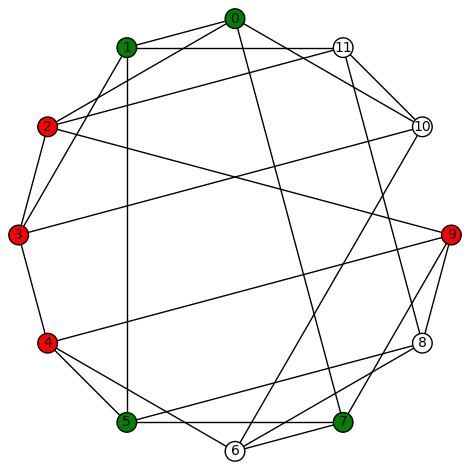
\includegraphics[height=5cm,width=5cm]{graphics/graph_d4reg12c_112221010200.png}
\end{center}
\begin{center}
%\vspace{8.0 cm}
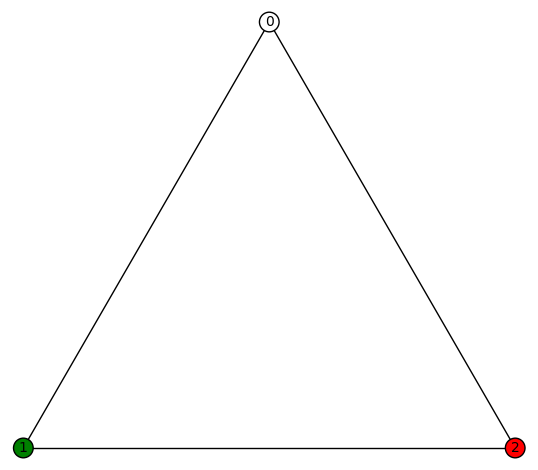
\includegraphics[height=4cm,width=4cm]{graphics/cycle3-012.png}
\end{center}
\end{minipage}
\caption{The quartic graph $\Gamma_2$ ({\tt d4reg12c}), with a degree four harmonic quotient morphism (indeed, a quasicover) to the graph $C_3=\Gamma_1=\Gamma_2/G$.}
\label{fig:harmonic-quotient_d4reg12c+C3}
\end{figure}



The remaining $108$ non-trivial harmonic quotient morphisms,
in the case $\Gamma_1$ has $2$ vertices, all map to
$\Gamma_1=P_2$.
}
\end{example}



\begin{example}% d4reg12d
  {\tt d4reg12d}\newline
\label{example:d4reg12d}  
{\rm  
  Let $\Gamma_2$ denote the graph {\tt d4reg12d} as given above.
It has $79$  non-trivial harmonic quotient morphisms
$\pi: \Gamma_2\to \Gamma_1=\Gamma_2/G$,
for some subgroup $G$ of $\Aut(\Gamma_2)$.
There are $3$ in the case $\Gamma_1$ has $8$ vertices,
$12$ in case $\Gamma_1$ has $7$ vertices,
only $1$ in case $\Gamma_1$ has $6$ vertices,
$9$ in case $\Gamma_1$ has $5$ vertices,
$9$ in case $\Gamma_1$ has $4$ vertices,
$25$ in the case $\Gamma_1$ has $3$ vertices,
and  $20$ in the case $\Gamma_1$ has $2$ vertices
(i.e., $\Gamma_1=P_2$).

All $3$ of the non-trivial harmonic quotient morphisms
$\pi: \Gamma_2\to \Gamma_1=\Gamma_2/G$, in the case where
$\Gamma_1$ has $8$ vertices, satisfy $\Gamma_1=$\verb+G?qipk+
(in the graph6 notation).
%\index{star graph}
For instance, when
\[
G = \langle  (1,11)(3,4)(6,8)(9,10) \rangle ,
\]
the quotient morphism $\pi$ (a homomorphism) maps to
$\Gamma_1=\Gamma_2/G =$\verb+G?qipk+
is tabulated below
and the uncolored graphs are depicted in
Figure \ref{fig:harmonic-quotient_d4reg12d+G_QU_qipk}. 

\begin{center}
\begin{tabular}{c|c|c|c}  
  $x$ & $\pi(x)$ & $m_\pi(x)$ & $\nu_\pi(x)$   \\ 
  0   &    7   &        2         &  0  \\ 
  1   &    3   &        1         &  0  \\ 
  2   &    1   &        2         &  0  \\ 
  3   &    0   &        1         &  0   \\
  4   &    0   &        1         &  0   \\
  5   &    6   &        2         &  0   \\
  6   &    5   &        1         &  0   \\
  7   &    4   &        2         &  0   \\
  8   &    5   &        1         &  0   \\
  9   &    2   &        1         &  0  \\   
  10  &    2  &        1         &  0  \\
  11  &    3   &        1         &  0  \\  
\end{tabular}
\end{center}

\[
  \genus(\Gamma_2) =13,\ \ \ \ \
  \genus(\Gamma_1) =5,
\]
\[
\deg(\phi) =2.
\]

\begin{figure}[H]
\begin{minipage}{\textwidth}
\begin{center}
%\vspace{8.0 cm}
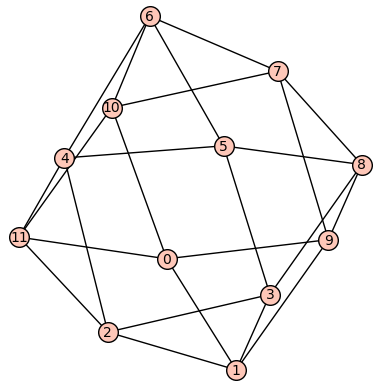
\includegraphics[height=5cm,width=5cm]{graphics/graph_d4reg12d2.png}
\end{center}
\begin{center}
%\vspace{8.0 cm}
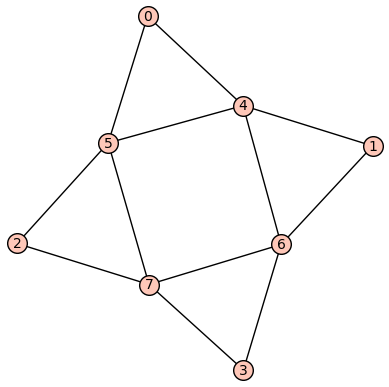
\includegraphics[height=4cm,width=4cm]{graphics/G_QU_qipk-quotient-of-d4reg12d.png}
\end{center}
\end{minipage}
\caption{The quartic graph $\Gamma_2$ ({\tt d4reg12d}), with a degree two harmonic quotient morphism (indeed, a homomorphism) to the graph $\Gamma_1=\Gamma_2/G$ as described above.}
\label{fig:harmonic-quotient_d4reg12d+G_QU_qipk}
\end{figure}

Of the $12$ non-trivial harmonic quotient morphisms
$\pi: \Gamma_2\to \Gamma_1=\Gamma_2/G$, in the case where
$\Gamma_1$ has $7$ vertices, exactly $6$ of them
satisfy $\Gamma_1=$\verb+FIe`w+. (These quotients have
vertical edges.)
The remaining $6$ satisfy $\Gamma_1=$\verb+FB]lg+
(in the graph6 notation).
%\index{star graph}
For instance, when
\[
G = \langle (1,10)(2,7)(3,6)(4,8)(9,11) \rangle ,
\]
the quotient morphism $\pi$ (a homomorphism) maps to
$\Gamma_1=\Gamma_2/G =$\verb+FB]lg+
is tabulated below
and the uncolored graphs are depicted in
Figure \ref{fig:harmonic-quotient_d4reg12d+FB_BR_lg}. 

\begin{center}
\begin{tabular}{c|c|c|c}  
  $x$ & $\pi(x)$ & $m_\pi(x)$ & $\nu_\pi(x)$   \\ 
  0   &    6   &        2         &  0  \\ 
  1   &    4   &        1         &  0  \\ 
  2   &    0   &        1         &  0  \\ 
  3   &    3   &        1         &  0   \\
  4   &    5   &        1         &  0   \\
  5   &    2   &        2         &  0   \\
  6   &    3   &        1         &  0   \\
  7   &    0   &        1         &  0   \\
  8   &    5   &        1         &  0   \\
  9   &    1   &        1         &  0  \\   
  10  &    4  &         1         &  0  \\
  11  &    1   &        1         &  0  \\  
\end{tabular}
\end{center}

\[
  \genus(\Gamma_2) =13,\ \ \ \ \
  \genus(\Gamma_1) =6,
\]
\[
\deg(\phi) =2.
\]

\begin{figure}[H]
\begin{minipage}{\textwidth}
\begin{center}
%\vspace{8.0 cm}
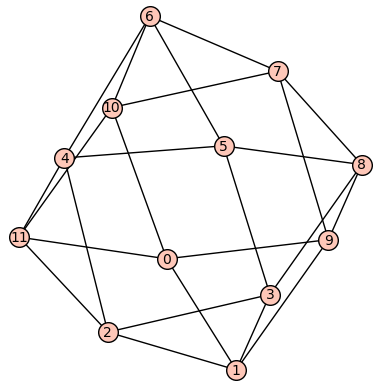
\includegraphics[height=5cm,width=5cm]{graphics/graph_d4reg12d2.png}
\end{center}
\begin{center}
%\vspace{8.0 cm}
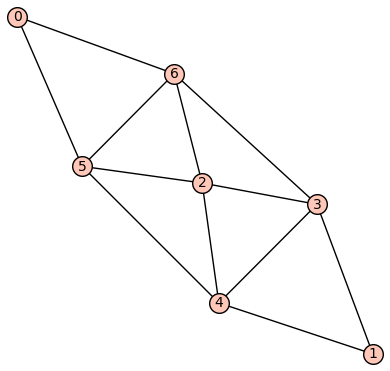
\includegraphics[height=4cm,width=4cm]{graphics/FB_BR_lg-quotient-of-d4reg12d.png}
\end{center}
\end{minipage}
\caption{The quartic graph $\Gamma_2$ ({\tt d4reg12d}), with a degree two harmonic quotient morphism (indeed, a homomorphism) to the graph $\Gamma_1=\Gamma_2/G$ as described above.}
\label{fig:harmonic-quotient_d4reg12d+FB_BR_lg}
\end{figure}


The only non-trivial harmonic quotient morphism
$\pi: \Gamma_2\to \Gamma_1=\Gamma_2/G$, in the case where
$\Gamma_1$ has $6$ vertices, satisfies $\Gamma_1={\tt Oct}$,
the quartic octahedral graph. (This quotient is a cover.)
\index{octahedral graph}
When
\[
G = \langle (0,5)(1,6)(2,7)(3,10)(4,9)(8,11) \rangle ,
\]
the quotient morphism $\pi$ maps to
$\Gamma_1=\Gamma_2/G ={\tt Oct}$
is tabulated below
and the uncolored graphs are depicted in
Figure \ref{fig:harmonic-quotient_d4reg12d+octahedral}. 

\begin{center}
\begin{tabular}{c|c|c|c}  
  $x$ & $\pi(x)$ & $m_\pi(x)$ & $\nu_\pi(x)$   \\ 
  0   &    5   &        1         &  0  \\ 
  1   &    4   &        1         &  0  \\ 
  2   &    2   &        1         &  0  \\ 
  3   &    3   &        1         &  0   \\
  4   &    1   &        1         &  0   \\
  5   &    5   &        1         &  0   \\
  6   &    4   &        1         &  0   \\
  7   &    2   &        1         &  0   \\
  8   &    0   &        1         &  0   \\
  9   &    1   &        1         &  0  \\   
  10  &    3  &         1         &  0  \\
  11  &    0   &        1         &  0  \\  
\end{tabular}
\end{center}

\[
  \genus(\Gamma_2) =13,\ \ \ \ \
  \genus(\Gamma_1) =7,
\]
\[
\deg(\phi) =2.
\]

\begin{figure}[H]
\begin{minipage}{\textwidth}
\begin{center}
%\vspace{8.0 cm}
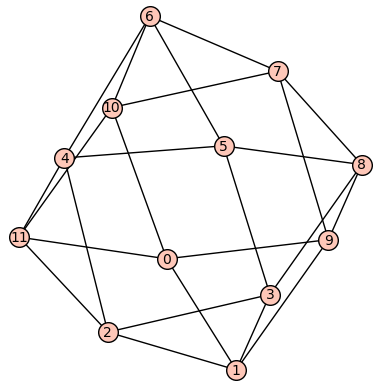
\includegraphics[height=5cm,width=5cm]{graphics/graph_d4reg12d2.png}
\end{center}
\begin{center}
%\vspace{8.0 cm}
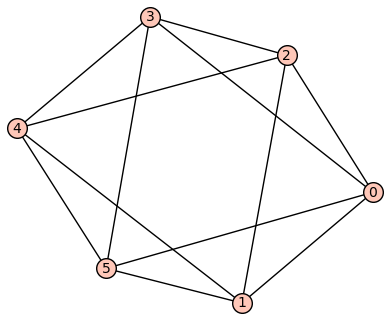
\includegraphics[height=4cm,width=4cm]{graphics/octahedral-quotient-of-d4reg12d.png}
\end{center}
\end{minipage}
\caption{The quartic graph $\Gamma_2$ ({\tt d4reg12d}), with a degree two harmonic quotient morphism (indeed, a cover) to the graph $\Gamma_1=\Gamma_2/G={\tt Oct}$.}
\label{fig:harmonic-quotient_d4reg12d+octahedral}
\end{figure}

Of the $9$ non-trivial harmonic quotient morphisms
$\pi: \Gamma_2\to \Gamma_1=\Gamma_2/G$, in the case where
$\Gamma_1$ has $5$ vertices, exactly $3$ of them
satisfy $\Gamma_1={\tt butterfly}$, the butterfly or bowtie graph.
(These quotients have no vertical edges.)
\index{butterfly graph}
\index{bowtie graph}
The remaining $6$ satisfy $\Gamma_1={\tt bull}$, the bull graph,
which can be invisioned as $C_3$ with two of the vertices having a
leaf\footnote{So if these leaves are pointing straight up
  and the degree 2 vertices is blwlow them, then the leafs look like
  horns and the degree 2 vertex looks like a chin.}.
\index{bull graph}
(These quotients do have vertical edges.)
When
\[
G = \langle (1,11)(3,4)(6,8)(9,10), (0,2)(1,11)(3,10)(4,9)(5,7)(6,8) \rangle ,
\]
the quotient morphism $\pi$ maps to
$\Gamma_1=\Gamma_2/G ={\tt butterfly}$
is tabulated below
and the uncolored graphs are depicted in
Figure \ref{fig:harmonic-quotient_d4reg12d+butterfly}. 

\begin{center}
\begin{tabular}{c|c|c|c}  
  $x$ & $\pi(x)$ & $m_\pi(x)$ & $\nu_\pi(x)$   \\
  0   &    1   &        2         &  0   \\
  1   &    4   &        2         &  0   \\
  2   &    1   &        2         &  0   \\
  3   &    0   &        1         &  0   \\
  4   &    0   &        1         &  0   \\
  5   &    2   &        2         &  0   \\
  6   &    3   &        2         &  0   \\
  7   &    2   &        2         &  0   \\
  8   &    3   &        2         &  0   \\
  9   &    0   &        1         &  0   \\
  10   &    0   &        1         &  0   \\
  11   &    4   &        2         &  0   \\
\end{tabular}
\end{center}

\[
  \genus(\Gamma_2) =13,\ \ \ \ \
  \genus(\Gamma_1) =2,
\]
\[
\deg(\phi) =4.
\]

\begin{figure}[H]
\begin{minipage}{\textwidth}
\begin{center}
%\vspace{8.0 cm}
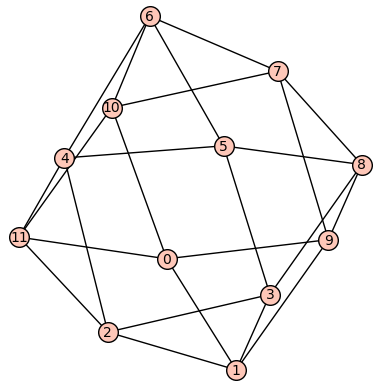
\includegraphics[height=5cm,width=5cm]{graphics/graph_d4reg12d2.png}
\end{center}
\begin{center}
%\vspace{8.0 cm}
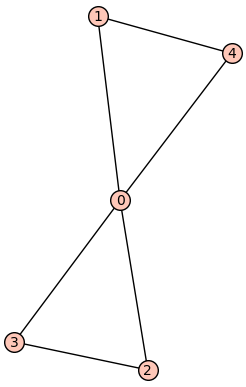
\includegraphics[height=4cm,width=4cm]{graphics/butterfly-quotient-of-d4reg12d.png}
\end{center}
\end{minipage}
\caption{The quartic graph $\Gamma_2$ ({\tt d4reg12d}), with a degree four harmonic quotient morphism (indeed, a homomorphism) to the graph $\Gamma_1=\Gamma_2/G={\tt butterfly}$.}
\label{fig:harmonic-quotient_d4reg12d+butterfly}
\end{figure}

Of the $9$ non-trivial harmonic quotient morphisms
$\pi: \Gamma_2\to \Gamma_1=\Gamma_2/G$, in the case where
$\Gamma_1$ has $4$ vertices, exactly $3$ of them
satisfy $\Gamma_1=C_4$, the cycle graph. 
The remaining $6$ satisfy $\Gamma_1={\tt diamond}$, the diamond graph.
\index{diamond graph}
(In each case, these quotients have vertical edges.)


Of the $25$ non-trivial harmonic quotient morphisms
$\pi: \Gamma_2\to \Gamma_1=\Gamma_2/G$, in the case where
$\Gamma_1$ has $3$ vertices, exactly $13$ of them
satisfy $\Gamma_1=P_3$, the path graph.
(In each case, these quotients have vertical edges.)
The remaining $12$ satisfy $\Gamma_1=C_3$, the cycle graph
($8$ distinct morphisms).
The quotients in this case $\pi: \Gamma_2\to C_3=\Gamma_2/G$
are multicovers of degree $8$ and multiplicity $m=2$.
When
\[
G = \langle 
(0,2)(1,11)(3,10)(4,9)(5,7)(6,8), (0,5)(1,8)(2,7)(3,9)(4,10)(6,11)\rangle ,
\]
the quotient morphism $\pi$ maps to
$\Gamma_1=\Gamma_2/G =C_3$
is tabulated below
and  depicted in Figure \ref{fig:harmonic-quotient_d4reg12d-C3_212002121001}.

\begin{center}
\begin{tabular}{c|c|c|c}  
  $x$ & $\pi(x)$ & $m_\pi(x)$ & $\nu_\pi(x)$   \\ 
  0   &    2   &        2         &  0  \\ 
  1   &    1   &        2         &  0  \\ 
  2   &    2   &        2         &  0  \\ 
  3   &    0   &        2         &  0   \\
  4   &    0   &        2         &  0   \\
  5   &    2   &        2         &  0   \\
  6   &    1   &        2         &  0   \\
  7   &    2   &        2         &  0   \\
  8   &    1   &        2         &  0   \\
  9   &    0   &        2         &  0  \\   
  10  &    0  &         2         &  0  \\
  11  &    1   &        2         &  0  \\  
\end{tabular}
\end{center}

\[
  \genus(\Gamma_2) =13,\ \ \ \ \
  \genus(\Gamma_1) =1,
\]
\[
\deg(\phi) =8.
\]

\begin{figure}[H]
\begin{minipage}{\textwidth}
\begin{center}
%\vspace{8.0 cm}
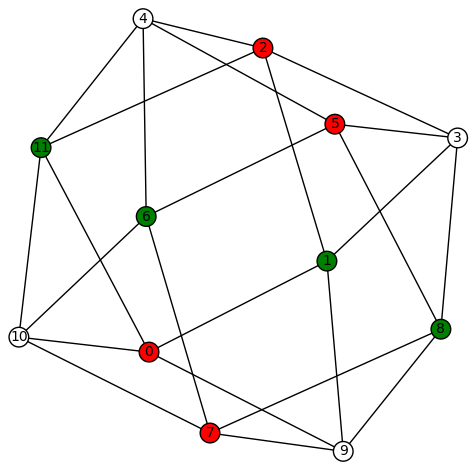
\includegraphics[height=5cm,width=5cm]{graphics/harmonic-quotient_d4reg12d-C3_212002121001b.png}
\end{center}
\begin{center}
%\vspace{8.0 cm}
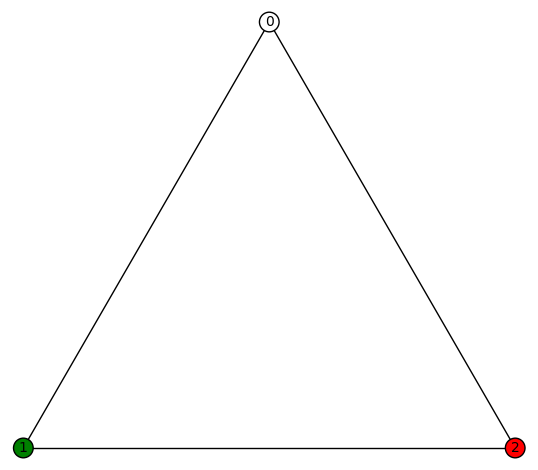
\includegraphics[height=4cm,width=4cm]{graphics/cycle3-012.png}
\end{center}
\end{minipage}
\caption{The quartic graph $\Gamma_2$ ({\tt d4reg12d}) is a degree eight $2$-multicover of $\Gamma_1=C_3$.}
\label{fig:harmonic-quotient_d4reg12d-C3_212002121001}
\end{figure}

All the $20$ non-trivial harmonic quotient morphisms
$\pi: \Gamma_2\to \Gamma_1=\Gamma_2/G$, in the case where
$\Gamma_1$ has $2$ vertices, map to $P_2$.

}
\end{example}



\begin{example}% d4reg12e
\label{example:d4reg12e}
 {\tt d4reg12e}\newline
{\rm  
  Let $\Gamma_2$ denote the graph {\tt d4reg12e} as given above.
It has $20$  non-trivial harmonic quotient morphisms
$\pi: \Gamma_2\to \Gamma_1=\Gamma_2/G$,
for some subgroup $G$ of $\Aut(\Gamma_2)$.
There are $6$ in the case $\Gamma_1$ has $7$ vertices,
only $1$ in case $\Gamma_1$ has $6$ vertices,
none in case $\Gamma_1$ has $5$ vertices,
$3$ in case $\Gamma_1$ has $4$ vertices,
$3$ in the case $\Gamma_1$ has $3$ vertices,
and  $7$ in the case $\Gamma_1$ has $2$ vertices
(i.e., $\Gamma_1=P_2$).

For instance, when
\[
G = \langle  (1,11)(2,9)(3,10)(5,6)(7,8) \rangle ,
\]
the quotient morphism maps to the graph
$\pi: \Gamma_2\to {\tt FKLkw}=\Gamma_1=\Gamma_2/G $ (in graph6 notation).
All of the $6$ quotients $\Gamma_1=\Gamma_2/G$ having $7$ vertices
are isomorphic to this graph, {\tt FKLkw}.
This example, which is a matchstick graph (see Remark~\ref{rem:matchstick}),
is tabulated below and the uncolored graphs are depicted in
Figure \ref{fig:harmonic-quotient_d4reg12e+FKLkw}.
\index{{\tt FKLkw} graph}

\begin{center}
\begin{tabular}{c|c|c|c}  
  $x$ & $\pi(x)$ & $m_\pi(x)$ & $\nu_\pi(x)$   \\ 
  0   &    5   &        2         &  0  \\ 
  1   &    2   &        1         &  0  \\ 
  2   &    3   &        1         &  0  \\ 
  3   &    4   &        1         &  1   \\
  4   &    0   &        2         &  0   \\
  5   &    1   &        1         &  0   \\
  6   &    1   &        1         &  0   \\
  7   &    6   &        1         &  1   \\
  8   &    6   &        1         &  1   \\
  9   &    3   &        1         &  0  \\   
  10  &    4  &         1         &  1  \\
  11  &    2   &        1         &  0  \\  
\end{tabular}
\end{center}

\[
  \genus(\Gamma_2) =13,\ \ \ \ \
  \genus(\Gamma_1) =5,
\]
\[
\deg(\phi) =2.
\]

\begin{figure}[H]
\begin{minipage}{\textwidth}
\begin{center}
%\vspace{8.0 cm}
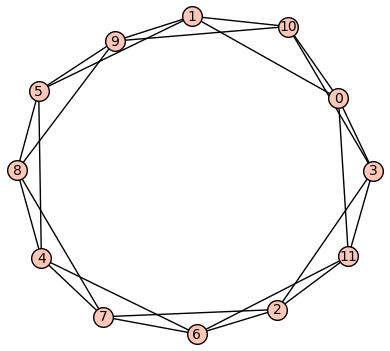
\includegraphics[height=5cm,width=5cm]{graphics/graph_d4reg12e1.png}
\end{center}
\begin{center}
%\vspace{8.0 cm}
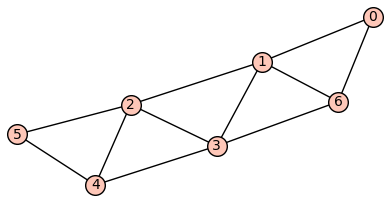
\includegraphics[height=4cm,width=4cm]{graphics/FKLkw-quotient-of-d4reg12e.png}
\end{center}
\end{minipage}
\caption{The quartic graph $\Gamma_2$, a degree two harmonic quotient to $\Gamma_1={\tt FKLkw}$.}
\label{fig:harmonic-quotient_d4reg12e+FKLkw}
\end{figure}

The only non-trivial harmonic quotient morphism
$\pi: \Gamma_2\to \Gamma_1=\Gamma_2/G$, in the case where
$\Gamma_1$ has $6$ vertices, satisfies $\Gamma_1={\tt Oct}$,
the quartic octahedral graph.
This quotient is also a cover\footnote{As in the above case of
{\tt d4reg12d}, see Example \ref{example:d4reg12d}.}
\index{octahedral graph}


The $3$ non-trivial harmonic quotient morphisms
$\pi: \Gamma_2\to \Gamma_1=\Gamma_2/G$, in the case where
$\Gamma_1$ has $4$ vertices, satisfy $\Gamma_1={\tt diamond}$,
the diamond graph.
\index{diamond graph}
When
\[
G = \langle 
(1,11)(2,9)(3,10)(5,6)(7,8),
(0,4)(1,5)(3,7)(6,11)(8,10)\rangle ,
\]
the quotient morphism $\pi$ mapping to
$\Gamma_1=\Gamma_2/G ={\tt diamond}$
is tabulated below
and  depicted in Figure \ref{fig:harmonic-quotient_d4reg12e-diamond_201320033130}.

\begin{center}
\begin{tabular}{c|c|c|c}  
  $x$ & $\pi(x)$ & $m_\pi(x)$ & $\nu_\pi(x)$   \\ 
  0   &    2   &        2         &  0  \\ 
  1   &    0   &        1         &  1  \\ 
  2   &    1   &        2         &  0  \\ 
  3   &    3   &        1         &  1   \\
  4   &    2   &        2         &  0   \\
  5   &    0   &        1         &  1   \\
  6   &    0   &        1         &  1   \\
  7   &    3   &        1         &  1   \\
  8   &    3   &        1         &  1   \\
  9   &    1   &        2         &  0  \\   
  10  &    3  &         1         &  1  \\
  11  &    0   &        1         &  1  \\  
\end{tabular}
\end{center}

\[
  \genus(\Gamma_2) =13,\ \ \ \ \
  \genus(\Gamma_1) =2,
\]
\[
\deg(\phi) =4.
\]

\begin{figure}[H]
\begin{minipage}{\textwidth}
\begin{center}
%\vspace{8.0 cm}
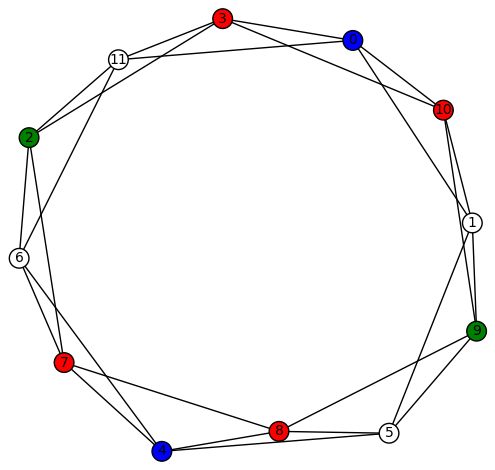
\includegraphics[height=5cm,width=5cm]{graphics/harmonic-quotient_d4reg12e-diamond_201320033130.png}
\end{center}
\begin{center}
%\vspace{8.0 cm}
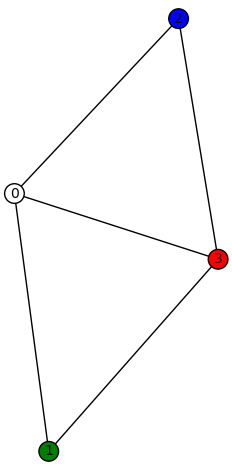
\includegraphics[height=4cm,width=4cm]{graphics/diamond-0123d.png}
\end{center}
\end{minipage}
\caption{The quartic graph $\Gamma_2$ ({\tt d4reg12e}) is a degree four quotient morphism to $\Gamma_1={\tt diamond}$.}
\label{fig:harmonic-quotient_d4reg12e-diamond_201320033130}
\end{figure}

The $3$ non-trivial harmonic quotient morphisms
$\pi: \Gamma_2\to \Gamma_1=\Gamma_2/G$, in the case where
$\Gamma_1$ has $3$ vertices,
satisfy $\Gamma_1=C_3$, the cycle graph.
These quotients $\pi: \Gamma_2\to C_3=\Gamma_2/G$
are multicovers\footnote{This too was seen in the above case of
{\tt d4reg12d}, see Example \ref{example:d4reg12d}.}
of degree $8$ and multiplicity $m=2$.

All the $7$ non-trivial harmonic quotient morphisms
$\pi: \Gamma_2\to \Gamma_1=\Gamma_2/G$, in the case where
$\Gamma_1$ has $2$ vertices, map to $P_2$.
}
\end{example}



\begin{example}% d4reg12f
\label{example:d4reg12f}
 {\tt d4reg12f}\newline
{\rm  
  Let $\Gamma_2$ denote the graph {\tt d4reg12f} as given above.
It has $76$  non-trivial harmonic quotient morphisms
$\pi: \Gamma_2\to \Gamma_1=\Gamma_2/G$,
for some subgroup $G$ of $\Aut(\Gamma_2)$.
There is exactly $1$ in the case $\Gamma_1$ has $8$ vertices,
none in case $\Gamma_1$ has $7$ vertices,
$16$ in case $\Gamma_1$ has $6$ vertices,
$30$ in case $\Gamma_1$ has $4$ vertices,
$6$ in the case $\Gamma_1$ has $3$ vertices,
and $23$ in the case $\Gamma_1$ has $2$ vertices
(i.e., $\Gamma_1=P_2$).

For instance, when
\[
G = \langle (1,8)(2,4)(3,10)(6,9)  \rangle ,
\]
the quotient morphism maps to the graph
$\pi: \Gamma_2\to $\verb+G?r@xw+$=\Gamma_1=\Gamma_2/G $ (in graph6 notation)
with degree sequence $[4,4,4,4,2,2,2,2]$. A very similar example occured in
Example \ref{example:d4reg12a}, where the quotient morphism
was also a graph homomorphism, so won't be tabulated here.

Of the $16$ non-trivial harmonic quotient morphisms
$\pi: \Gamma_2\to \Gamma_1=\Gamma_2/G$, in the case where
$\Gamma_1$ has $6$ vertices, exactly $8$ of them
satisfy $\Gamma_1=$\verb+EL~o+ (in graph6 notation).
(In each case, these quotients all seem to be quasicovers.)
The remaining $8$ satisfy $\Gamma_1=$\verb+E@JW+.

For instance, when
\[
G = \langle (0,7)(1,3)(2,6)(4,9)(5,11)(8,10) \rangle ,
\]
the quotient morphism maps to the graph
$\pi: \Gamma_2\to $\verb+EL~o+$=\Gamma_1=\Gamma_2/G $ (in graph6 notation).
This is tabulated below and the uncolored graphs are depicted in
Figure \ref{fig:harmonic-quotient_d4reg12f+EL_tilde_o}.
\index{\verb+EL~o+ graph}

\begin{center}
\begin{tabular}{c|c|c|c}  
  $x$ & $\pi(x)$ & $m_\pi(x)$ & $\nu_\pi(x)$   \\ 
  0   &    2   &        1         &  0  \\ 
  1   &    5   &        1         &  1  \\ 
  2   &    3   &        1         &  0  \\ 
  3   &    5   &        1         &  1   \\
  4   &    4   &        1         &  0   \\
  5   &    1   &        1         &  0   \\
  6   &    3   &        1         &  0   \\
  7   &    2   &        1         &  0   \\
  8   &    0   &        1         &  1   \\
  9   &    4   &        1         &  0  \\   
  10  &    0  &         1         &  1  \\
  11  &    1   &        1         &  0  \\  
\end{tabular}
\end{center}

\[
  \genus(\Gamma_2) =13,\ \ \ \ \
  \genus(\Gamma_1) =6,
\]
\[
\deg(\phi) =2.
\]

\begin{figure}[H]
\begin{minipage}{\textwidth}
\begin{center}
%\vspace{8.0 cm}
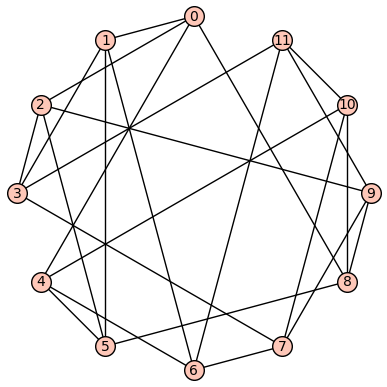
\includegraphics[height=5cm,width=5cm]{graphics/graph_d4reg12f.png}
\end{center}
\begin{center}
%\vspace{8.0 cm}
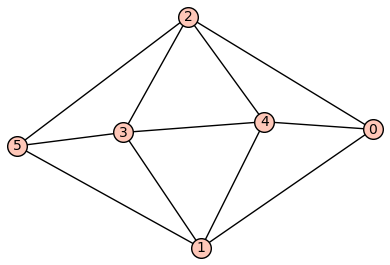
\includegraphics[height=4cm,width=4cm]{graphics/EL_tilde_o-quotient-of-d4reg12f.png}
\end{center}
\end{minipage}
\caption{The quartic graph $\Gamma_2$ ({\tt d4reg12f}), a degree two harmonic quotient to $\Gamma_1={\tt EL~o}$.}
\label{fig:harmonic-quotient_d4reg12f+EL_tilde_o}
\end{figure}

For instance, when
\[
G = \langle (1,2)(4,8)(6,9)(7,11), (1,8)(2,4)(3,10)(6,9) \rangle ,
\]
the quotient morphism maps to the graph
$\pi: \Gamma_2\to $\verb+E@JW+$=\Gamma_1=\Gamma_2/G $ (in graph6 notation). This graph is sometimes called the {\it R graph},
because it can be drawn to look like the letter R.
Further, this quotient morphism is in fact a graph homomorphism
(without vertical edges).
This is tabulated below and the uncolored graphs are depicted in
Figure \ref{fig:harmonic-quotient_d4reg12f+E_at_JW}.
\index{\verb+E@JW+ graph}
\index{``R'' graph}

\begin{center}
\begin{tabular}{c|c|c|c}  
  $x$ & $\pi(x)$ & $m_\pi(x)$ & $\nu_\pi(x)$   \\ 
  0   &    5   &        4         &  0  \\ 
  1   &    0   &        1         &  0  \\ 
  2   &    0   &        1         &  0  \\ 
  3   &    4   &        2         &  0   \\
  4   &    0   &        1         &  0   \\
  5   &    2   &        4         &  0   \\
  6   &    1   &        2         &  0   \\
  7   &    3   &        2         &  0   \\
  8   &    0   &        1         &  0   \\
  9   &    1   &        2         &  0  \\   
  10  &    4  &         2         &  0  \\
  11  &    3   &        2         &  0  \\  
\end{tabular}
\end{center}

\[
  \genus(\Gamma_2) =13,\ \ \ \ \
  \genus(\Gamma_1) =1,
\]
\[
\deg(\phi) =4.
\]

\begin{figure}[H]
\begin{minipage}{\textwidth}
\begin{center}
%\vspace{8.0 cm}
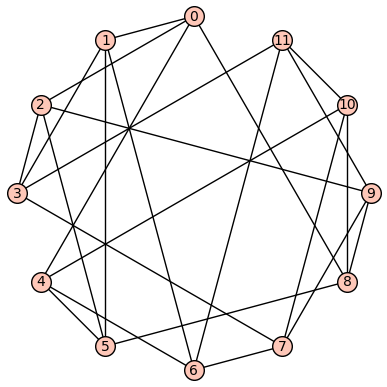
\includegraphics[height=5cm,width=5cm]{graphics/graph_d4reg12f.png}
\end{center}
\begin{center}
%\vspace{8.0 cm}
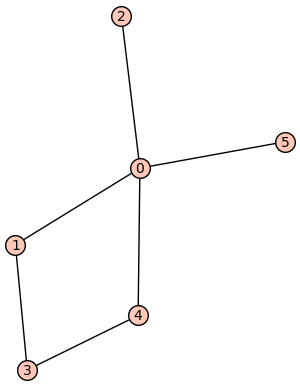
\includegraphics[height=4cm,width=4cm]{graphics/E_at_JW-quotient-of-d4reg12f.png}
\end{center}
\end{minipage}
\caption{The quartic graph $\Gamma_2$ ({\tt d4reg12f}), a degree 4 harmonic quotient to the R graph, $\Gamma_1$.}
\label{fig:harmonic-quotient_d4reg12f+E_at_JW}
\end{figure}


Of the $30$ non-trivial harmonic quotient morphisms
$\pi: \Gamma_2\to \Gamma_1=\Gamma_2/G$, in the case where
$\Gamma_1$ has $4$ vertices, exactly $4$ of them
satisfy $\Gamma_1={\tt diamond}$.
The remaining $26$ satisfy $\Gamma_1=P_4$.
In each case, these quotients to the path graph $P_4$ all seem
to be graph homomorphisms.
\index{diamond graph}


For instance, when
\[
G = \langle (1,8)(2,4)(3,10)(6,9), (0,5)(1,4,8,2)(3,6,10,9)(7,11) \rangle ,
\]
the quotient morphism maps to the graph
$\pi: \Gamma_2\to P_4=\Gamma_1=\Gamma_2/G $.
Further, this quotient morphism is in fact a graph homomorphism
(without vertical edges).
This is tabulated below and depicted in
Figure \ref{fig:harmonic-quotient_d4reg12f-P4_311213201220}.

\begin{center}
\begin{tabular}{c|c|c|c}  
  $x$ & $\pi(x)$ & $m_\pi(x)$ & $\nu_\pi(x)$   \\ 
  0   &    3   &        4         &  0  \\ 
  1   &    1   &        2         &  0  \\ 
  2   &    1   &        2         &  0  \\ 
  3   &    2   &        2         &  0   \\
  4   &    1   &        2         &  0   \\
  5   &    3   &        4         &  0   \\
  6   &    2   &        2         &  0   \\
  7   &    0   &        4         &  0   \\
  8   &    1   &        2         &  0   \\
  9   &    2   &        2         &  0  \\   
  10  &    2  &         2         &  0  \\
  11  &    0   &        4         &  0  \\  
\end{tabular}
\end{center}

\[
  \genus(\Gamma_2) =13,\ \ \ \ \
  \genus(\Gamma_1) =0,
\]
\[
\deg(\phi) =8.
\]

\begin{figure}[H]
\begin{minipage}{\textwidth}
\begin{center}
%\vspace{8.0 cm}
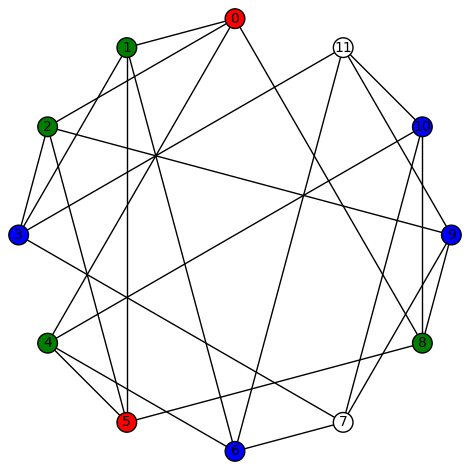
\includegraphics[height=5cm,width=5cm]{graphics/harmonic-quotient_d4reg12f-P4_311213201220.png}
\end{center}
\begin{center}
%\vspace{8.0 cm}
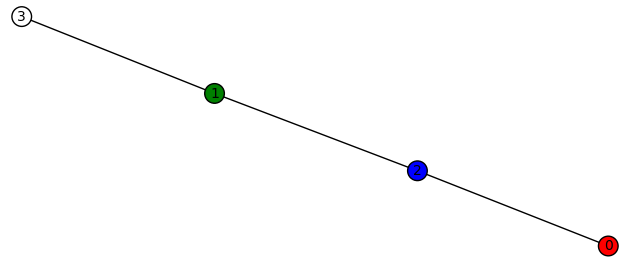
\includegraphics[height=4cm,width=4cm]{graphics/path4-3120.png}
\end{center}
\end{minipage}
\caption{The quartic graph $\Gamma_2$ ({\tt d4reg12f}), a degree 8 harmonic quotient to the path graph, $\Gamma_1=P_4$.}
\label{fig:harmonic-quotient_d4reg12f-P4_311213201220}
\end{figure}

All the $6$ non-trivial harmonic quotient morphisms
$\pi: \Gamma_2\to \Gamma_1=\Gamma_2/G$, in the case where
$\Gamma_1$ has $3$ vertices, map to $P_3$.

All $23$ of the non-trivial harmonic quotient morphisms
$\pi: \Gamma_2\to \Gamma_1=\Gamma_2/G$, in the case where
$\Gamma_1$ has $2$ vertices, map to $P_2$.
}
\end{example}


  
\section{Quintic cases}
\label{sec:quintic-examples}

This section treats connected quintic graphs with $6$, $8$ and $10$
vertices. For $10$ vertices only a selection of the graphs is included.


\subsection{\texorpdfstring{$6$}{6} vertices}

This subsection describes the connected quintic graphs on $6$ vertices.
It records their invariants and harmonic morphism counts, and then
works out harmonic quotient morphisms in examples.


Only the complete graph $K_6$ fits into this category.

There are exactly $90$ non-trivial harmonic morphisms from
$K_6$ to $K_3=C_3$. All of these morphisms are quasi-multicovers
of degree $4$, constant horizontal multiplicity $2$ and
constant vertical mutiplicity $1$.
%See Example \ref{example:K6-K3} for an example.
\index{quasi-multicover}


\subsubsection{Examples}

Each example below takes one graph from the list above and describes
its harmonic quotient morphisms.


\begin{example}% d5reg6a
\label{example:d5reg6a}
  {\tt d5reg6a}\newline
{\rm  
  Let $\Gamma_2=K_6$. All $90$ of the quasi-multicovers
of $C_3$ (with degree $4$, constant horizontal multiplicity $2$,
constant vertical mutiplicity $1$) are obtained as a harmonic
quotient morphism $\pi:\Gamma_2 \to \Gamma_1=\Gamma_2/G$, for some
subgroup $G\subset \Aut(\Gamma_2)$.

}
\end{example}

\subsection{\texorpdfstring{$8$}{8} vertices}
\label{sec:d5reg8}

This subsection describes the connected quintic graphs on $8$ vertices.
It records their invariants and harmonic morphism counts, and then
works out harmonic quotient morphisms in examples.


There are exactly three $5$-regular graphs with $8$ vertices, two of which are vertex transitive.
They are Hamiltonian by Ore's Theorem.


\begin{enumerate}
\item
  {\tt d5reg8a}\newline
  Define the graph  $\Gamma$
  % d5reg8-1 = d5reg8a
  to have edge set:

\[
E = \{
(0, 1), (0, 2), (0, 4), (0, 6), (0, 7), (1, 2), (1, 3), (1, 4), (1, 5), (2, 3),
\]
\[
(2, 5), (2, 7), (3, 4), (3, 6), (3, 7), (4, 5), (4, 6), (5, 6), (5, 7), (6, 7)
\}.
\]
It has diameter $2$,
girth $3$, circumference $8$, 
critical group of size $21025 = 5^2 29^2$, 
and automorphism group of size $60$. This has chromatic number $4$.

There are $6$ non-trivial harmonic morphisms from $\Gamma$ to $P_3$,
but none to $P_4$, $C_3$, $C_4$, or to $K_4$.

\item
  {\tt d5reg8b}\newline
Define the graph  $\Gamma$ to have edge set:
% d5reg8-2 = d5reg8b
  

\[
E = \{
(0, 1), (0, 2), (0, 3), (0, 5), (0, 6), (1, 2), (1, 3), (1, 4), (1, 7), (2, 3), 
\]
\[
(2, 4), (2, 7), (3, 5), (3, 6), (4, 5), (4, 6), (4, 7), (5, 6), (5, 7), (6, 7)
\}.
\]
This graph is isomorphic to the strong graph product
$C_4\times_{Str} P_2$. It has diameter $2$,
girth $3$, circumference $8$, 
critical group of size $20736 = 2^8 3^4$, 
and automorphism group of size $128$. This is a vertex transitive graph but not
edge transitive.
This has chromatic number $4$.
\index{vertex transitive graph}

There are $4$ non-trivial harmonic morphisms from $\Gamma$ to $P_3$,
$48$ non-trivial harmonic morphisms from $\Gamma$ to $C_3$, and
$8$ non-trivial harmonic
morphisms\footnote{Moreover, it appears all of these are quasi-multicovers
  (with constant horizontal multiplicity $2$ and constant vertical
  multiplicity $1$). This is consistent with the values predicted by
the known values for the projection morphism $pr_1:C_4\times_{Str}P_2 \to C_4$.}
\index{quasi-multicover}
from $\Gamma$ to $C_4$. However, there are
no non-trivial harmonic morphisms from $\Gamma$ to $P_4$ or to $K_4$.


\item
  {\tt d5reg8c}\newline
  Define the graph  $\Gamma$
  % d5reg8-3 = d5reg8c
  to have edge set:

\[
E = \{
(0, 1), (0, 2), (0, 3), (0, 4), (0, 6), (1, 2), (1, 3), (1, 5), (1, 6), (2, 3),
\]
\[
(2, 5), (2, 7), (3, 4), (3, 7), (4, 5), (4, 6), (4, 7), (5, 6), (5, 7), (6, 7)
\}.
\]
It has diameter $2$,
girth $3$, circumference $8$, 
critical group of size $20808 = 2^3 3^2 17^2$, 
and automorphism group of size $16$. This is a vertex transitive graph but not
edge transitive.
This has chromatic number $4$.
\index{vertex transitive graph}

There are $12$ non-trivial harmonic morphisms from $\Gamma$ to $C_3$.
However, there are no non-trivial harmonic morphisms from $\Gamma$ to $P_3$,
$P_4$, $C_4$, or to $K_4$.


\end{enumerate}



\subsubsection{Examples}

Each example below takes one graph from the list above and describes
its harmonic quotient morphisms.


\begin{example}% d5reg8a
\label{example:d5reg8a}
  {\tt d5reg8a}\newline
{\rm  
  Let $\Gamma_2$ denote the graph {\tt d5reg8a}, as above.
It has $7$  non-trivial harmonic quotient morphisms
$\pi: \Gamma_2\to \Gamma_1=\Gamma_2/G$,
for some subgroup $G$ of $\Aut(\Gamma_2)$.
There are exactly $2$ in the case $\Gamma_1$ has $4$ vertices,
and $5$ in the case $\Gamma_1$ has $2$ vertices (one of them for $G=\Aut(\Gamma_2)$)
(i.e., $\Gamma_1=P_2$).
Both of the quotient morphisms in case $\Gamma_1$ has $4$ vertices
are to $\Gamma_1=St_4$. 

For instance, when
\[
G = \langle (1,2,7,6,4) \rangle ,
\]
the quotient morphism maps to the graph
$\pi: \Gamma_2\to St_4=\Gamma_1=\Gamma_2/G $
This is tabulated below.

\begin{center}
\begin{tabular}{c|c|c|c}  
  $x$ & $\pi(x)$ & $m_\pi(x)$ & $\nu_\pi(x)$   \\ 
  0   &    2   &        5         &  0  \\ 
  1   &    1   &        1         &  2  \\ 
  2   &    1   &        1         &  2  \\ 
  3   &    0   &        5         &  0   \\
  4   &    1   &        1         &  2   \\
  5   &    3   &        5         &  0   \\
  6   &    1   &        1         &  2   \\
  7   &    1   &        1         &  2   \\
\end{tabular}
\end{center}

\[
  \genus(\Gamma_2) =13,\ \ \ \ \
  \genus(\Gamma_1) =0,
\]
\[
\deg(\phi) =5.
\]
  
}
\end{example}


\begin{example}% d5reg8b
  \label{example:d5reg8b}
  {\tt d5reg8b}\newline
{\rm  
  Let $\Gamma_2$ denote the graph {\tt d5reg8b}, as above.
It has $304$  non-trivial harmonic quotient morphisms
$\pi: \Gamma_2\to \Gamma_1=\Gamma_2/G$,
for some subgroup $G$ of $\Aut(\Gamma_2)$.
There are exactly $26$ in the case $\Gamma_1$ has $4$ vertices,
$116$ in the case $\Gamma_1$ has $3$ vertices
and $162$ in the case $\Gamma_1$ has $2$ vertices
(i.e., $\Gamma_1=P_2$).
All of the quotient morphisms in case $\Gamma_1$ has $4$ vertices
are to $\Gamma_1=C_4$. 
  When
\[
G = \langle (0,3)(1,2)(4,7)(5,6) \rangle ,
\]
the quotient morphism $\pi$ maps to
$\Gamma_1=\Gamma_2/G =C_4$
is tabulated below
and  depicted in Figure \ref{fig:harmonic-quotient_d5reg8b-C4_32231001}.

\begin{center}
\begin{tabular}{c|c|c|c}  
  $x$ & $\pi(x)$ & $m_\pi(x)$ & $\nu_\pi(x)$   \\ 
  0   &    3   &        2         &  1  \\ 
  1   &    2   &        2         &  1  \\ 
  2   &    2   &        2         &  1  \\ 
  3   &    3   &        2         &  1   \\
  4   &    1   &        2         &  1   \\
  5   &    0   &        2         &  1   \\
  6   &    0   &        2         &  1   \\
  7   &    1   &        2         &  1   \\
\end{tabular}
\end{center}

\[
  \genus(\Gamma_2) =13,\ \ \ \ \
  \genus(\Gamma_1) =1,
\]
\[
\deg(\phi) =4.
\]

\begin{figure}[H]
\begin{minipage}{\textwidth}
\begin{center}
%\vspace{8.0 cm}
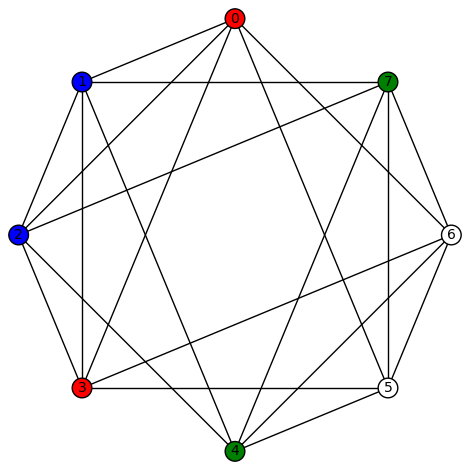
\includegraphics[height=5cm,width=5cm]{graphics/harmonic-quotient_d5reg8b-C4_32231001.png}
\end{center}
\begin{center}
%\vspace{8.0 cm}
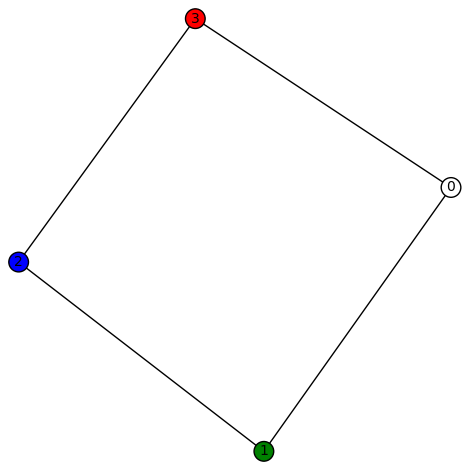
\includegraphics[height=4cm,width=4cm]{graphics/Cycle4-0123c.png}
\end{center}
\end{minipage}
\caption{The quintic graph $\Gamma_2$ ({\tt d5reg8b}) is a degree four quasi-multicover of $\Gamma_1=C_4$.}
\label{fig:harmonic-quotient_d5reg8b-C4_32231001}
\end{figure}

Of the $116$ quotient morphisms in case
$\Gamma_1$ has $3$ vertices, $24$ are to $\Gamma_1=C_3$ ($8$ distinct morphisms)
and $92$ are to $P_3$ ($2$ distinct morphisms).
The quotients to $C_3$ are not quasi-multicovers.
For example, when
\[
G = \langle (4,7)(5,6), (0,1)(2,3)(4,6,7,5) \rangle ,
\]
the quotient morphism $\pi$ maps to
$\Gamma_1=\Gamma_2/G =C_3$
is tabulated below
and  depicted in Figure \ref{fig:harmonic-quotient_d5reg8b-C3_00112222}.

\begin{center}
\begin{tabular}{c|c|c|c}  
  $x$ & $\pi(x)$ & $m_\pi(x)$ & $\nu_\pi(x)$   \\ 
  0   &    0   &        2         &  1  \\ 
  1   &    0   &        2         &  1  \\ 
  2   &    1   &        2         &  1  \\ 
  3   &    1   &        2         &  1   \\
  4   &    2   &        1         &  3   \\
  5   &    2   &        1         &  3   \\
  6   &    2   &        1         &  3   \\
  7   &    2   &        1         &  3   \\
\end{tabular}
\end{center}

\[
  \genus(\Gamma_2) =13,\ \ \ \ \
  \genus(\Gamma_1) =1,
\]
\[
\deg(\phi) =4.
\]

\begin{figure}[H]
\begin{minipage}{\textwidth}
\begin{center}
%\vspace{8.0 cm}
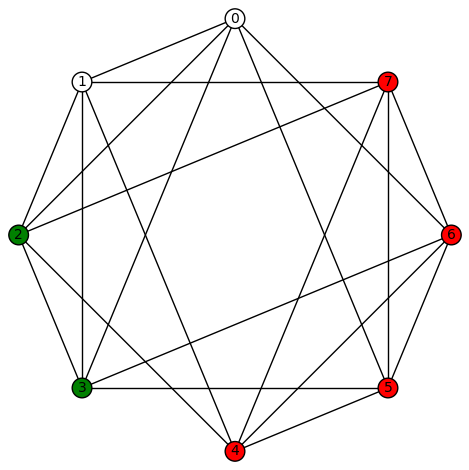
\includegraphics[height=5cm,width=5cm]{graphics/harmonic-quotient_d5reg8b-C3_00112222.png}
\end{center}
\begin{center}
%\vspace{8.0 cm}
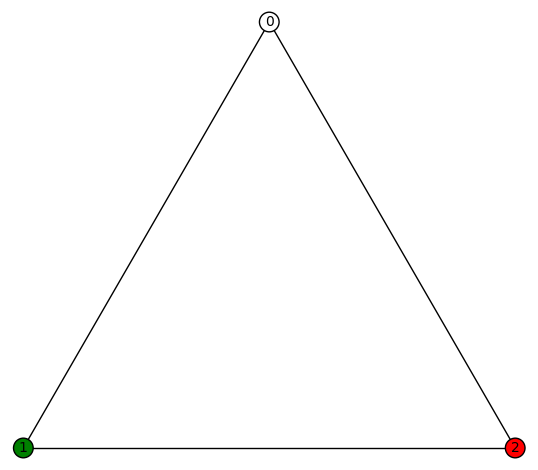
\includegraphics[height=4cm,width=4cm]{graphics/cycle3-012.png}
\end{center}
\end{minipage}
\caption{The quintic graph $\Gamma_2$ ({\tt d5reg8b}) has a degree four harmonic quotient morphism to $\Gamma_1=C_3$.}
\label{fig:harmonic-quotient_d5reg8b-C3_00112222}
\end{figure}

}
\end{example}


\begin{example}% d5reg8c
\label{example:d5reg8c}
  {\tt d5reg8c}\newline
{\rm  
  Let $\Gamma_2$ denote the graph {\tt d5reg8c}, as above.
It has $6$  non-trivial harmonic quotient morphisms
$\pi: \Gamma_2\to \Gamma_1=\Gamma_2/G$,
for some subgroup $G$ of $\Aut(\Gamma_2)$.
There are exactly $2$ in the case $\Gamma_1$ has $3$ vertices,
and $4$ in the case $\Gamma_1$ has $2$ vertices
(i.e., $\Gamma_1=P_2$).
The morphisms to $C_3$ are very similar to those of the
previous Example \ref{example:d5reg8b} and will not be repeated.
  
}
\end{example}




\subsection{\texorpdfstring{$10$}{10} vertices}

This subsection describes a selection of the connected quintic graphs on $10$ vertices.
It records their invariants and harmonic morphism counts, and then
works out harmonic quotient morphisms in examples.


Up to isomorphism, there are exactly $60$ $5$-regular graphs with $10$ vertices, four of which are vertex transitive,
% d5reg10-12, -24, -39
and exactly one
% d5reg10-53 
of those which is also edge transitive (and that one is also symmetric, distance regular, and bipartite). By Ore's Theorem, these are all Hamiltonian.



\begin{enumerate}
\item
  {\tt d5reg10a}\newline
  Define the graph  $\Gamma$
  % d5reg10-12 = d5reg10a
to have edge set:

\[
E = \{
(0, 1), (0, 2), (0, 3), (0, 8), (0, 9), (1, 2), (1, 3), (1, 5), (1, 9), (2, 3),
\]
\[
(2, 7), (2, 9), (3, 6), (3, 9), (4, 5), (4, 6), (4, 7), (4, 8), (4, 9), (5, 6),
\]
\[
(5, 7), (5, 8), (6, 7), (6, 8), (7, 8)
\}.
\]
It has diameter $2$,
girth $3$, circumference $10$, 
critical group of size $300125 = 5^3 7^4$, 
and automorphism group of size $240$. This is a vertex transitive graph but not
edge transitive.
This has chromatic number $5$.
\index{vertex transitive graph}

There are no non-trivial harmonic morphisms from $\Gamma$ to $P_3$, $P_4$, $C_3$, $C_4$, or to $K_4$.


\item
  {\tt d5reg10b}\newline
  Define the graph  $\Gamma$
  % d5reg10-24 = d5reg10b
  to have edge set:

\[
E = \{
(0, 1), (0, 6), (0, 7), (0, 8), (0, 9), (1, 3), (1, 4), (1, 5),(1, 7), (2, 3),
\]
\[
(2, 5), (2, 7), (2, 8), (2, 9), (3, 6), (3, 8), (3, 9), (4, 5), (4, 7), (4, 8),
\]
\[
(4, 9), (5, 6), (5, 9), (6, 7), (6, 8)
\}.
\]
It has diameter $2$,
girth $3$, circumference $10$, 
critical group of size $360375 = 3\cdot 5^3 31^2$, 
and automorphism group of size $20$. This is a vertex transitive graph but not
edge transitive.
This has chromatic number $4$.
\index{vertex transitive graph}

There are no non-trivial harmonic morphisms from $\Gamma$ to $P_3$, $P_4$, $C_3$, $C_4$, or to $K_4$.

\item
  {\tt d5reg10c}\newline
  Define the graph $\Gamma$
  % d5reg10-39 = d5reg10c
to have edge set:

\[
E = \{
(0, 1), (0, 2), (0, 7), (0, 8), (0, 9), (1, 2), (1, 3), (1, 5), (1, 9), (2, 3),
\]
\[
(2, 5), (2, 9), (3, 4), (3, 5), (3, 6), (4, 5), (4, 6), (4, 7), (4, 8), (5, 6), \]
\[
(6, 7), (6, 8), (7, 8), (7, 9), (8, 9)
\}.
\]
It has diameter $2$,
girth $3$, circumference $10$, 
critical group of size $311040 = 2^8 3^5 5$, 
and automorphism group of size $320$. This is a vertex transitive graph but not
edge transitive.
This has chromatic number $5$.
\index{vertex transitive graph}

There are $10$ non-trivial harmonic morphisms from $\Gamma$ to $P_3$
and $60$ non-trivial harmonic morphisms from $\Gamma$ to $C_3$.
However, there are
no non-trivial harmonic morphisms from $\Gamma$ to $P_4$, $C_4$, or to $K_4$.


\item
  {\tt d5reg10d}\newline
  Define the graph  $\Gamma$
  % d5reg10-53 = d5reg10d
to have edge set:

\[
E = \{
(0, 1), (0, 2), (0, 5), (0, 6), (0, 8), (1, 3), (1, 4), (1, 7), (1, 9), (2, 3),
\]
\[
(2, 4), (2, 7), (2, 9), (3, 5), (3, 6), (3, 8), (4, 5), (4, 6), (4, 8), (5, 7),
\]
\[
(5, 9), (6, 7), (6, 9), (7, 8), (8, 9)
\}.
\]
It has diameter $2$,
girth $4$, circumference $10$, 
critical group of size $390625 = 5^8$, 
and automorphism group of size $28800$.
This is a vertex transitive, edge transitive,
symmetric (=arc transitive), and distance regular.
This has chromatic number $2$ (bipartite).
It is a circulant graph with parameters $(10, [1, 3, 5, 7, 9])$
and is isomorphic to the complete bipartite graph $K_{5,5}$.
\index{complete bipartite graph}
\index{vertex transitive graph}
\index{edge transitive graph}
\index{arc transitive graph}
\index{bipartite graph}
\index{distance regular graph}

There are no non-trivial harmonic morphisms from $\Gamma$ to
$P_4$, $C_3$, $C_4$, or to $K_4$. However, there
are\footnote{One of these has CL $(0, 1, 1, 1, 1, 1, 1, 1, 1, 2)$,
yielding a weed with three roots (see Remark~\ref{rem:weed}).}
$100$ non-trivial harmonic morphisms from $\Gamma$ to $P_3$.

\end{enumerate}


\subsubsection{Examples}

Each example below takes one graph from the list above and describes
its harmonic quotient morphisms.


\begin{example}% d5reg10a
\label{example:d5reg10a}
  {\tt d5reg10a}\newline
{\rm  
  Let $\Gamma_2$ denote the graph {\tt d5reg10a}, as above.
It has $151$  non-trivial harmonic quotient morphisms
$\pi: \Gamma_2\to \Gamma_1=\Gamma_2/G$,
for some subgroup $G$ of $\Aut(\Gamma_2)$.
There is exactly $1$ in the case $\Gamma_1$ has $5$ vertices
(in which case $\Gamma_1=K_5$),
and $150$ in the case $\Gamma_1$ has $2$ vertices
(i.e., $\Gamma_1=P_2$).
\index{complete graph}

The quotient morphism for the
subgroup\footnote{In this example, the subgroup $G$
is actually the center of $\Aut(\Gamma_2)$.}

\[
G=\langle (0,8)(1,5)(2,7)(3,6)(4,9) \rangle,
\]
is tabulated below. The uncolored graphs are depicted in
Figure \ref{fig:harmonic-quotient_d5reg10a+K5}.

\begin{center}
\begin{tabular}{c|c|c|c}  
  $x$ & $\phi(x)$ & $m_\phi(x)$ & $\nu_\phi(x)$ \\ \hline
  0   &    4   &        1         &  1   \\ 
  1   &    0   &        1         &  1  \\ 
  2   &    3   &        1         &  1  \\ 
  3   &    2   &        1         &  1  \\ 
  4   &    1   &        1         &  1   \\ 
  5   &    0   &        1         &  1    \\ 
  6   &    2   &        1         &  1   \\ 
  7   &    3   &        1         &  1   \\
  8   &    4   &        1         &  1   \\
  9   &    1   &        1         &  1   \\
\end{tabular}
\end{center}

\[
  \genus(\Gamma_2) =16,\ \ \ \ \
  \genus(\Gamma_1) =6,
\]

\[
\deg(\phi) =2.
\]

\begin{figure}[H]
\begin{minipage}{\textwidth}
\begin{center}
%\vspace{8.0 cm}
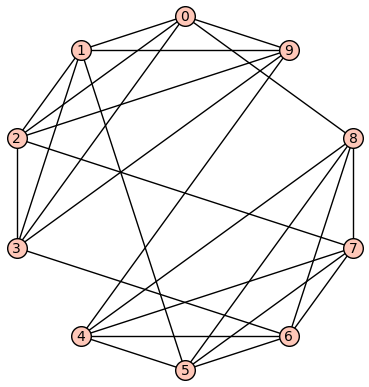
\includegraphics[height=5cm,width=5cm]{graphics/graph_d5reg10a.png}
\end{center}
\begin{center}
%\vspace{8.0 cm}
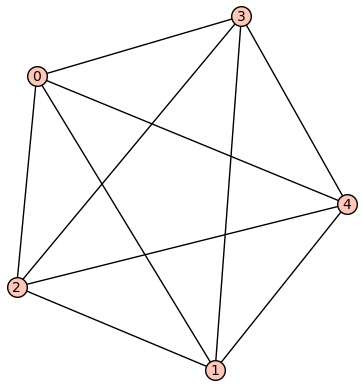
\includegraphics[height=4cm,width=4cm]{graphics/K5-quotient-of-d5reg10a.png}
\end{center}
\end{minipage}
\caption{The quintic graph  $\Gamma_2$ ({\tt d5reg10a}) is a degree two quasicover of the complete graph, $\Gamma_1=\Gamma_2/G_2=K_5$.}
\label{fig:harmonic-quotient_d5reg10a+K5}
\end{figure}

In this example, $G$ is the center of $\Aut(\Gamma_2)$ and
$\Aut(\Gamma_2)/G=\Aut(\Gamma_1)=\Aut(K_5)=S_5$.

\noindent
{\bf Question}:
Is the quotient

\[
\pi: \Gamma_2 \to K_5=\Gamma_1=\Gamma_2/G
\]
an $S_5$-equivariant morphism (that is to say, the morphism commutes with the
group actions)?


}
\end{example}


\begin{example}% d5reg10b
\label{example:d5reg10b}
  {\tt d5reg10b}\newline
{\rm  
  Let $\Gamma_2$ denote the graph {\tt d5reg10b}, as above.
It has $3$  non-trivial harmonic quotient morphisms
$\pi: \Gamma_2\to \Gamma_1=\Gamma_2/G$,
for some subgroup $G$ of $\Aut(\Gamma_2)$.
There is exactly $1$ in the case $\Gamma_1$ has $5$ vertices
(in which case $\Gamma_1=K_5$),
and $2$ in the case $\Gamma_1$ has $2$ vertices
(i.e., $\Gamma_1=P_2$).
\index{complete graph}

This example is similar in some ways to {\tt d5reg10a}, except that
it's automorphism group is much smaller. For example, in this
example, $K_5$ is also the quotient of $\Gamma_2$ by the
center of $\Aut(\Gamma_2)$. Moreover, the quotient morphism
in this case is also a degree two quasicover
where each edge has vertical multiplicity $1$.


}
\end{example}


\begin{example}% d5reg10c
\label{example:d5reg10c}
  {\tt d5reg10c}\newline
{\rm  
  Let $\Gamma_2$ denote the graph {\tt d5reg10c}, as above.
It has $730$  non-trivial harmonic quotient morphisms
$\pi: \Gamma_2\to \Gamma_1=\Gamma_2/G$,
for some subgroup $G$ of $\Aut(\Gamma_2)$.
There are $158$ in the case $\Gamma_1$ has $5$ vertices
(all of these have $\Gamma_1=C_5$),
$540$ in the case $\Gamma_1$ has $3$ vertices
(all of these have $\Gamma_1=P_3$),
and $32$ in the case $\Gamma_1$ has $2$ vertices
(i.e., $\Gamma_1=P_2$).

The quotient morphism for the
subgroup\footnote{In this example, the subgroup $G$
is actually the center of $\Aut(\Gamma_2)$.}

\[
G=\langle (0,9)(1,2)(3,5)(4,6)(7,8) \rangle,
\]
is tabulated below. The uncolored graphs are depicted in
Figure \ref{fig:harmonic-quotient_d5reg10c+C5}.

\begin{center}
\begin{tabular}{c|c|c|c}  
  $x$ & $\phi(x)$ & $m_\phi(x)$ & $\nu_\phi(x)$ \\ \hline
  0   &    3   &        2         &  1   \\ 
  1   &    2   &        2         &  1  \\ 
  2   &    2   &        2         &  1  \\ 
  3   &    1   &        2         &  1  \\ 
  4   &    0   &        2         &  1   \\ 
  5   &    1   &        2         &  1    \\ 
  6   &    0   &        2         &  1   \\ 
  7   &    4   &        2         &  1   \\
  8   &    4   &        2         &  1   \\
  9   &    3   &        2         &  1   \\
\end{tabular}
\end{center}

\[
  \genus(\Gamma_2) =16,\ \ \ \ \
  \genus(\Gamma_1) =1,
\]

\[
\deg(\phi) =4.
\]

\begin{figure}[H]
\begin{minipage}{\textwidth}
\begin{center}
%\vspace{8.0 cm}
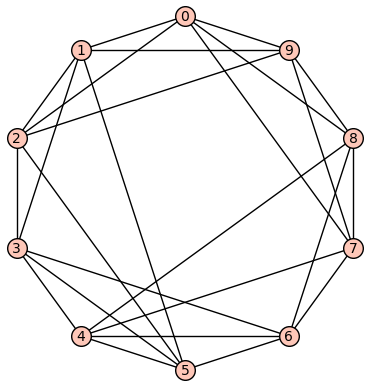
\includegraphics[height=5cm,width=5cm]{graphics/graph_d5reg10c.png}
\end{center}
\begin{center}
%\vspace{8.0 cm}
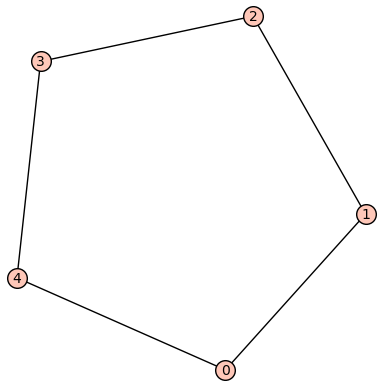
\includegraphics[height=4cm,width=4cm]{graphics/C5-quotient-of-d5reg10c.png}
\end{center}
\end{minipage}
\caption{The quintic graph  $\Gamma_2$ ({\tt d5reg10c}) is a degree four quasi-$2$-multicover of the cycle graph, $\Gamma_1=\Gamma_2/G_2=C_5$.}
\label{fig:harmonic-quotient_d5reg10c+C5}
\end{figure}

The quotient morphism for the
subgroup\footnote{In this example, the subgroup $G$
contains the center of $\Aut(\Gamma_2)$ as a subgroup of index $2$.}

\[
G=\langle (1,7)(2,8)(3,4)(5,6), (0,9)(1,2)(3,5)(4,6)(7,8) \rangle,
\]
is tabulated below. 

\begin{center}
\begin{tabular}{c|c|c|c}  
  $x$ & $\phi(x)$ & $m_\phi(x)$ & $\nu_\phi(x)$ \\ \hline
  0   &    2   &        4         &  1   \\ 
  1   &    1   &        2         &  1  \\ 
  2   &    1   &        2         &  1  \\ 
  3   &    0   &        2         &  3  \\ 
  4   &    0   &        2         &  3   \\ 
  5   &    0   &        2         &  3    \\ 
  6   &    0   &        2         &  3   \\ 
  7   &    1   &        2         &  1   \\
  8   &    1   &        2         &  1   \\
  9   &    2   &        4         &  1   \\
\end{tabular}
\end{center}

\[
  \genus(\Gamma_2) =16,\ \ \ \ \
  \genus(\Gamma_1) =0,
\]

\[
\deg(\phi) =8.
\]


}
\end{example}


\begin{example}% d5reg10d
\label{example:d5reg10d}
  {\tt d5reg10d}\newline
{\rm  
  Let $\Gamma_2$ denote the graph {\tt d5reg10d}, as above.
It has $28425$  non-trivial harmonic quotient morphisms
$\pi: \Gamma_2\to \Gamma_1=\Gamma_2/G$,
for some subgroup $G$ of $\Aut(\Gamma_2)$.
There are $40$ in the case $\Gamma_1$ has $6$ vertices
(all of these have $\Gamma_1=St_6$),
$120$ in the case $\Gamma_1$ has $5$ vertices
(all of these have $\Gamma_1=K_5$),
and $28265$ in the case $\Gamma_1$ has $2$ vertices
(i.e., $\Gamma_1=P_2$).

The quotient morphism for the
subgroup\footnote{Here $\Aut(\Gamma_2)$ has trivial center. The group $G$ is a cyclic
group of order $5$ acting on one side of the bipartition and fixing the other.}

\[
G=\langle (1,5,8,2,6) \rangle,
\]
is tabulated below. The uncolored graphs are depicted in
Figure \ref{fig:harmonic-quotient_d5reg10d+St6}.

\begin{center}
\begin{tabular}{c|c|c|c}  
  $x$ & $\phi(x)$ & $m_\phi(x)$ & $\nu_\phi(x)$ \\ \hline
  0   &    4   &        5         &  0   \\ 
  1   &    1   &        1         &  0  \\ 
  2   &    1   &        1         &  0  \\ 
  3   &    0   &        5         &  0  \\ 
  4   &    3   &        5         &  0   \\ 
  5   &    1   &        1         &  0    \\ 
  6   &    1   &        1         &  0   \\ 
  7   &    5   &        5         &  0   \\
  8   &    1   &        1         &  0   \\
  9   &    2   &        5         &  0   \\
\end{tabular}
\end{center}

\[
  \genus(\Gamma_2) =16,\ \ \ \ \
  \genus(\Gamma_1) =0,
\]

\[
\deg(\phi) =5.
\]

\begin{figure}[H]
\begin{minipage}{\textwidth}
\begin{center}
%\vspace{8.0 cm}
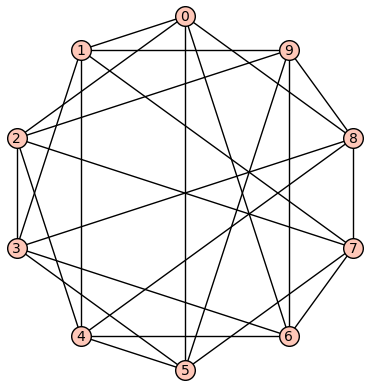
\includegraphics[height=5cm,width=5cm]{graphics/graph_d5reg10d.png}
\end{center}
\begin{center}
%\vspace{8.0 cm}
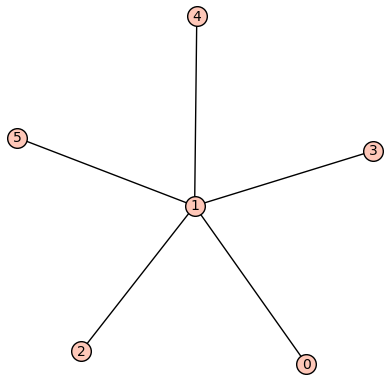
\includegraphics[height=4cm,width=4cm]{graphics/St6-quotient-of-d5reg10d.png}
\end{center}
\end{minipage}
\caption{The quintic graph  $\Gamma_2$ ({\tt d5reg10d}) is a degree five quotient homomorphism to the star graph, $\Gamma_1=\Gamma_2/G_2=St_6$.}
\label{fig:harmonic-quotient_d5reg10d+St6}
\end{figure}

This example is also similar in some ways to {\tt d5reg10a}
in Example \ref{example:d5reg10a}, except that
its automorphism group is much larger. In this
example, $K_5$ is also the quotient of $\Gamma_2$ by
a subgroup of $\Aut(\Gamma_2)$ of order $2$. Moreover, the quotient morphism
in this case is also a degree two quasicover
where each edge has vertical multiplicity $1$.
}
\end{example}



\section{Summary of results}
\label{sec:summary}

This section collects what the examples show about harmonic quotients of
small regular graphs and lists some open questions. All statements are
computational results (Section~\ref{sec:computations}).

The catalogue contains $86$ graphs: $40$ cubic, $38$ quartic and $8$
quintic. The table below gives, for each of them, the order of
$\Aut(\Gamma_2)$ and the number $N$ of subgroups $G\neq 1$ whose quotient
morphism is harmonic and non-constant (Section~\ref{sec:quotients}).

\begin{center}
\small
\begin{tabular}{lrr|lrr|lrr}
\hline
graph & $|\Aut|$ & $N$ & graph & $|\Aut|$ & $N$ & graph & $|\Aut|$ & $N$ \\
\hline
{\tt d3reg6a} & 12 & 6 & {\tt d3reg12d} & 32 & 0 & {\tt d4reg9i} & 16 & 5 \\
{\tt d3reg6b} & 72 & 50 & {\tt d3reg12e} & 4 & 2 & {\tt d4reg10a} & 8 & 2 \\
{\tt d3reg8a} & 16 & 14 & {\tt d3reg12f} & 8 & 0 & {\tt d4reg10b} & 4 & 2 \\
{\tt d3reg8b} & 4 & 2 & {\tt d3reg12g} & 4 & 0 & {\tt d4reg10c} & 2 & 0 \\
{\tt d3reg8c} & 12 & 2 & {\tt d3reg12h} & 64 & 53 & {\tt d4reg10d} & 20 & 8 \\
{\tt d3reg8d} & 48 & 55 & {\tt d3reg12i} & 16 & 2 & {\tt d4reg10e} & 320 & 850 \\
{\tt d3reg8e} & 16 & 7 & {\tt d3reg12j} & 16 & 15 & {\tt d4reg10f} & 240 & 251 \\
{\tt d3reg10a} & 32 & 4 & {\tt d3reg12k} & 2 & 0 & {\tt d4reg11a} & 288 & 12 \\
{\tt d3reg10b} & 4 & 0 & {\tt d3reg12l} & 24 & 10 & {\tt d4reg11b} & 2 & 0 \\
{\tt d3reg10c} & 8 & 0 & {\tt d3reg12m} & 24 & 31 & {\tt d4reg11c} & 22 & 0 \\
{\tt d3reg10d} & 16 & 0 & {\tt d3reg12n} & 48 & 35 & {\tt d4reg11d} & 22 & 0 \\
{\tt d3reg10e} & 16 & 2 & {\tt d4reg5a} & 120 & 75 & {\tt d4reg11e} & 1 & 0 \\
{\tt d3reg10f} & 2 & 1 & {\tt d4reg6a} & 48 & 59 & {\tt d4reg11f} & 64 & 30 \\
{\tt d3reg10g} & 12 & 2 & {\tt d4reg7a} & 14 & 0 & {\tt d4reg11g} & 144 & 9 \\
{\tt d3reg10h} & 2 & 0 & {\tt d4reg7b} & 48 & 28 & {\tt d4reg12a} & 768 & 7195 \\
{\tt d3reg10i} & 4 & 0 & {\tt d4reg8a} & 16 & 10 & {\tt d4reg12b} & 24 & 21 \\
{\tt d3reg10j} & 6 & 0 & {\tt d4reg8b} & 48 & 46 & {\tt d4reg12c} & 144 & 142 \\
{\tt d3reg10k} & 4 & 2 & {\tt d4reg8c} & 1152 & 2221 & {\tt d4reg12d} & 48 & 79 \\
{\tt d3reg10l} & 6 & 0 & {\tt d4reg8d} & 16 & 12 & {\tt d4reg12e} & 24 & 20 \\
{\tt d3reg10m} & 8 & 5 & {\tt d4reg8e} & 4 & 2 & {\tt d4reg12f} & 64 & 76 \\
{\tt d3reg10n} & 48 & 32 & {\tt d4reg8f} & 12 & 3 & {\tt d5reg6a} & 720 & 715 \\
{\tt d3reg10o} & 8 & 3 & {\tt d4reg9a} & 12 & 12 & {\tt d5reg8a} & 60 & 7 \\
{\tt d3reg10p} & 4 & 2 & {\tt d4reg9b} & 2 & 1 & {\tt d5reg8b} & 128 & 304 \\
{\tt d3reg10q} & 20 & 13 & {\tt d4reg9c} & 18 & 4 & {\tt d5reg8c} & 16 & 6 \\
{\tt d3reg10r} & 20 & 8 & {\tt d4reg9d} & 4 & 0 & {\tt d5reg10a} & 240 & 151 \\
{\tt d3reg10s} & 120 & 27 & {\tt d4reg9e} & 12 & 6 & {\tt d5reg10b} & 20 & 3 \\
{\tt d3reg12a} & 16 & 0 & {\tt d4reg9f} & 18 & 4 & {\tt d5reg10c} & 320 & 730 \\
{\tt d3reg12b} & 16 & 0 & {\tt d4reg9g} & 72 & 59 & {\tt d5reg10d} & 28800 & 28425 \\
{\tt d3reg12c} & 8 & 0 & {\tt d4reg9h} & 32 & 4 &  & &  \\
\hline
\end{tabular}
\end{center}

\paragraph{Graphs with no harmonic quotient.}
Twenty-one of the $86$ graphs have no non-constant harmonic quotient
morphism at all. They are the following.
\begin{center}
\begin{tabular}{lllllll}
{\tt d3reg10b} & {\tt d3reg10c} & {\tt d3reg10d} & {\tt d3reg10h} & {\tt d3reg10i} & {\tt d3reg10j} & {\tt d3reg10l} \\
{\tt d3reg12a} & {\tt d3reg12b} & {\tt d3reg12c} & {\tt d3reg12d} & {\tt d3reg12f} & {\tt d3reg12g} & {\tt d3reg12k} \\
{\tt d4reg7a} & {\tt d4reg9d} & {\tt d4reg10c} & {\tt d4reg11b} & {\tt d4reg11c} & {\tt d4reg11d} & {\tt d4reg11e} \\
\end{tabular}
\end{center}
 A small automorphism group is one reason.
For example, {\tt d4reg11e} has trivial automorphism group. But it is not
the only reason. The automorphism group of {\tt d3reg12d} has order $32$.
Three of the twenty-one graphs are vertex transitive. They are the
circulants {\tt d4reg7a} $\cong C_7(1,2)$, {\tt d4reg11c} $\cong C_{11}(1,3)$
and {\tt d4reg11d} $\cong C_{11}(1,2)$. Each has an automorphism group of
order $2p$, where $p$ is the number of vertices.

\paragraph{Graphs whose harmonic quotients all go to $P_2$.}
Among the $86$ graphs, only $K_5$ ({\tt d4reg5a}) has harmonic quotients
and has them all with target $P_2$. This is a partial answer to the
Question in Section~\ref{sec:introduction}. The graph {\tt d5reg10b} comes
close. Its three harmonic quotients are one to $K_5$ and two to $P_2$.

\paragraph{Many subgroups, few morphisms.}
Different subgroups often give the same quotient morphism. For
{\tt d4reg12a}, $1330$ subgroups give one and the same quotient morphism to
$C_6$. For {\tt d4reg10e} and {\tt d5reg10c}, $158$ subgroups give one and
the same quotient morphism to $C_5$.

\paragraph{Open questions.}
\begin{enumerate}
\item The Question of Section~\ref{sec:introduction} remains open beyond
the graphs listed here.
\item For which circulant graphs of prime order $p$, with automorphism group
of order $2p$, is some quotient morphism harmonic? The only subgroups of
such a group with more than one orbit are the subgroups of order $2$, each generated by a reflection.
\item Which regular graphs with a large automorphism group have no
harmonic quotient? Among cubic graphs, {\tt d3reg12d} is the example here
with the largest automorphism group (order $32$).
\end{enumerate}

\section{Glossary}
\label{sec:glossary}

This section defines the technical terms used in the paper, in
alphabetical order.

\begin{description}
\item[arc transitive] The automorphism group acts transitively on ordered
pairs of adjacent vertices. Also called symmetric.
\item[barbell graph] $\mathrm{Barbell}(n_1,n_2)$ is two copies of $K_{n_1}$
joined by a path with $n_2$ interior vertices.
\item[circulant graph] A graph on $\mathbb{Z}/n\mathbb{Z}$ in which each
vertex $i$ is adjacent to $i\pm j$ for $j$ in a fixed set $L$. Written
$C_n(L)$ or ``circulant with parameters $(n,L)$''.
\item[circumference] The length of a longest cycle.
\item[CL format] The list $(\phi(0),\dots,\phi(n-1))$ that describes a
morphism.
\item[cover, quasicover, multicover] See Definition~\ref{def:covers}.
\item[critical group] The Jacobian $\Jac(\Gamma)$ of a graph. Its order is
the number of spanning trees.
\item[degree] Of a harmonic morphism: the number of edges over any edge of
the target (Section~\ref{sec:harmonic-morphisms}).
\item[distance regular] For any two vertices $u$, $v$ at distance $d$, the
numbers of neighbors of $v$ at distance $d-1$, $d$ and $d+1$ from $u$ depend
only on $d$.
\item[edge transitive] The automorphism group acts transitively on edges.
\item[genus] $|E|-|V|+1$ for a connected graph. Also called the cyclomatic
number or first Betti number.
\item[girth] The length of a shortest cycle.
\item[graph6] A compact text format for graphs \cite{Mc26}.
\item[Hamiltonian] Having a cycle through every vertex.
\item[harmonic morphism] See Definition~\ref{def:harmonic}.
\item[harmonic quotient] A quotient morphism $\Gamma_2\to\Gamma_2/G$ that is
harmonic (Section~\ref{sec:quotients}).
\item[homomorphism] A harmonic morphism with no vertical edges.
\item[horizontal multiplicity] $m_\phi(x)$ in Definition~\ref{def:harmonic}.
\item[integral graph] A graph whose adjacency eigenvalues are all integers.
\item[LCF notation] A description of a cubic Hamiltonian graph
(Section~\ref{sec:graph-data}).
\item[non-trivial] Of a harmonic morphism: not constant.
\item[standard form] Vertices $0,\dots,n-1$ and edges $(u,v)$ with $u<v$.
\item[strongly regular] A regular graph in which adjacent vertices have
$\lambda$ common neighbors and non-adjacent vertices have $\mu$ common
neighbors, for fixed $\lambda$ and $\mu$.
\item[vertex transitive] The automorphism group acts transitively on
vertices.
\item[vertical edge, vertical multiplicity] An edge whose ends have the
same image, and the number $\nu_\phi(x)$ of such edges at $x$.
\end{description}

\section*{Acknowledgments}
\addcontentsline{toc}{section}{Acknowledgments}

Claude (Anthropic, model Claude Opus 5.5) refereed the original draft for
correctness in November 2026. It recomputed every table, count and graph
invariant with independent programs, found the errors corrected in this
revision, and proposed the corrections. It also prepared this draft to the
authors' style guide. It wrote the introduction, literature review,
background, notation, summary, glossary and these acknowledgments, and it
checked the bibliography against the sources. AI review is not an
independent certification of the results. The authors are responsible for
the content.

\begin{thebibliography}{99}
\raggedright

\bibitem[AM25]{AM25}
K. Archer and C. Melles,
{\it Harmonic morphisms of arithmetical structures on graphs},
preprint, 2025, \url{https://arxiv.org/abs/2504.08539}.

\bibitem[BC76]{BC76}
F. C. Bussemaker and D. M. Cvetkovi\'c,
{\it There are exactly 13 connected, cubic, integral graphs},
Univ. Beograd. Publ. Elektrotehn. Fak. Ser. Mat. Fiz. No.~544--576 (1976),
43--48.

\bibitem[BN09]{BN09}
M. Baker and S. Norine,
{\it Harmonic morphisms and hyperelliptic graphs},
Int. Math. Res. Not. IMRN 2009, no.~15, 2914--2955.
Preprint version: \url{https://arxiv.org/abs/0707.1309}.

\bibitem[Co11]{Co11}
S. Corry,
{\it Genus bounds for harmonic group actions on finite graphs},
Int. Math. Res. Not. IMRN 2011, no.~19, 4515--4533.

\bibitem[Co12]{Co12}
S. Corry,
{\it Harmonic Galois theory for finite graphs},
in: Galois--Teichm\"uller Theory and Arithmetic Geometry,
Adv. Stud. Pure Math. 63 (2012), 121--140.

\bibitem[Co15]{Co15}
S. Corry,
{\it Maximal harmonic group actions on finite graphs},
Discrete Math. 338 (2015), 784--792.

\bibitem[dR26]{dR26}
H. N. de Ridder et al.,
{\it Information System on Graph Classes and their Inclusions (ISGCI)},
\url{https://www.graphclasses.org}, accessed November 2026.

\bibitem[GAP]{GAP}
The GAP Group,
{\it GAP -- Groups, Algorithms, and Programming}, version 4.16.1,
\url{https://www.gap-system.org}.

\bibitem[JM17]{JM17}
W. D. Joyner and C. G. Melles,
{\it Adventures in Graph Theory},
Applied and Numerical Harmonic Analysis, Birkh\"auser, Cham, 2017.

\bibitem[Mc26]{Mc26}
B. D. McKay,
{\it Graph formats},
\url{https://users.cecs.anu.edu.au/~bdm/data/formats.html},
accessed November 2026.

\bibitem[MJ22]{MJ22}
C. Melles and D. Joyner,
{\it Hitchhiker's handbook to harmonic morphisms},
manuscript in preparation, 2022.

\bibitem[MJ26]{MJ26}
C. Melles and D. Joyner,
{\it Exploring Graphs via Harmonic Morphisms},
Springer Nature, forthcoming.

\bibitem[MM19]{MM19}
A. D. Mednykh and I. A. Mednykh,
{\it The number of spanning trees in circulant graphs, its arithmetic
properties and asymptotic},
Discrete Math. 342 (2019), 1772--1781.
Preprint version: \url{https://arxiv.org/abs/1711.00175}.

\bibitem[MP14]{MP14}
B. D. McKay and A. Piperno,
{\it Practical graph isomorphism, II},
J. Symbolic Comput. 60 (2014), 94--112.

\bibitem[MZ23]{MZ23}
M. Meyer and D. Zakharov,
{\it Chip-firing on graphs of groups},
preprint, 2023, \url{https://arxiv.org/abs/2307.03348}.

\bibitem[Sage]{Sage}
The Sage Developers,
{\it SageMath, the Sage Mathematics Software System},
\url{https://www.sagemath.org}.

\bibitem[Ur00]{Ur00}
H. Urakawa,
{\it A discrete analogue of the harmonic morphism and Green kernel
comparison theorems},
Glasgow Math. J. 42 (2000), 319--334.

\bibitem[VZ24]{VZ24}
M. Vetluzhskikh and D. Zakharov,
{\it Critical groups in harmonic abelian quotients},
preprint, 2024, \url{https://arxiv.org/abs/2409.04629}.

\end{thebibliography}


\printindex

\end{document}
